% Generated by scripts/plot_results.py. % Generated by scripts/plot_results.py. % Generated by scripts/plot_results.py. % Generated by scripts/plot_results.py. \input{figures/figures.tex} or copy single blocks.

\begin{figure}[htbp]
  \centering
  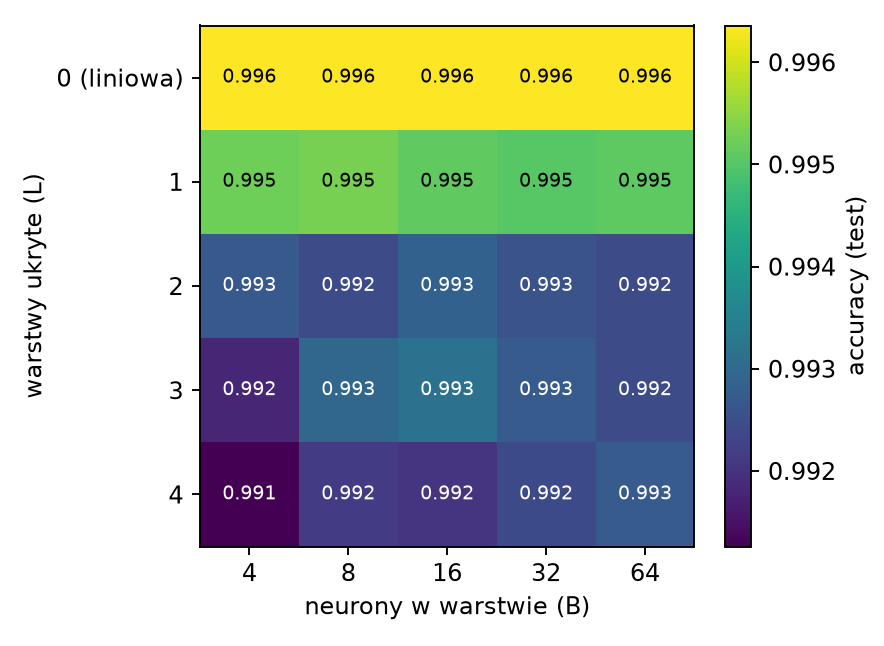
\includegraphics[width=0.7\linewidth]{figures/simple/arch_heatmap_test_accuracy.png}
  \caption{simple: accuracy (test) (mediana) w zależności od liczby warstw ukrytych $L$ i neuronów w warstwie $B$.}
  \label{fig:simple:arch_heatmap_test_accuracy}
\end{figure}

\begin{figure}[htbp]
  \centering
  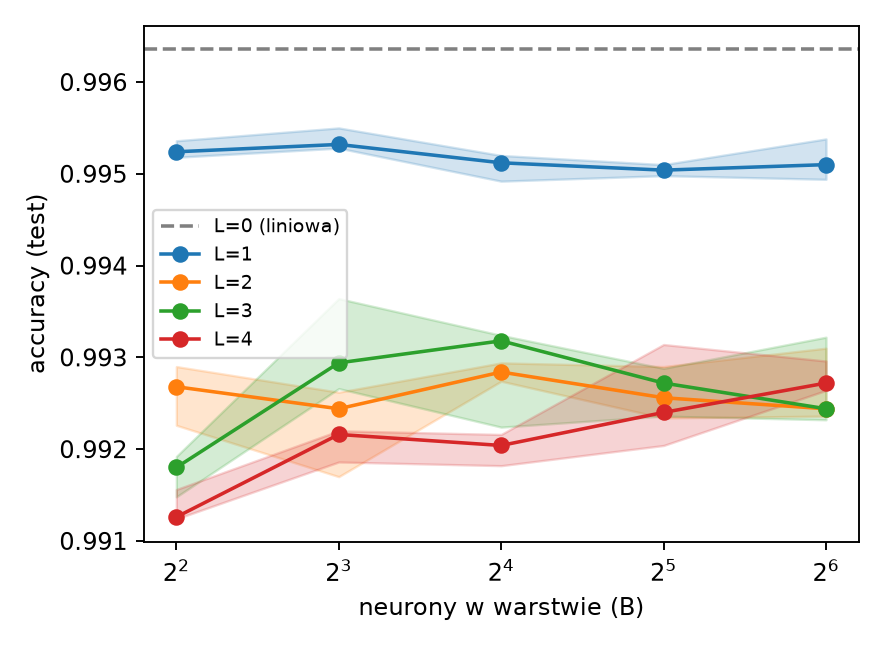
\includegraphics[width=0.7\linewidth]{figures/simple/arch_lines_test_accuracy.png}
  \caption{simple: accuracy (test) w zależności od $B$ dla każdej liczby warstw $L$ (mediana i kwartyle po ziarnach).}
  \label{fig:simple:arch_lines_test_accuracy}
\end{figure}

\begin{figure}[htbp]
  \centering
  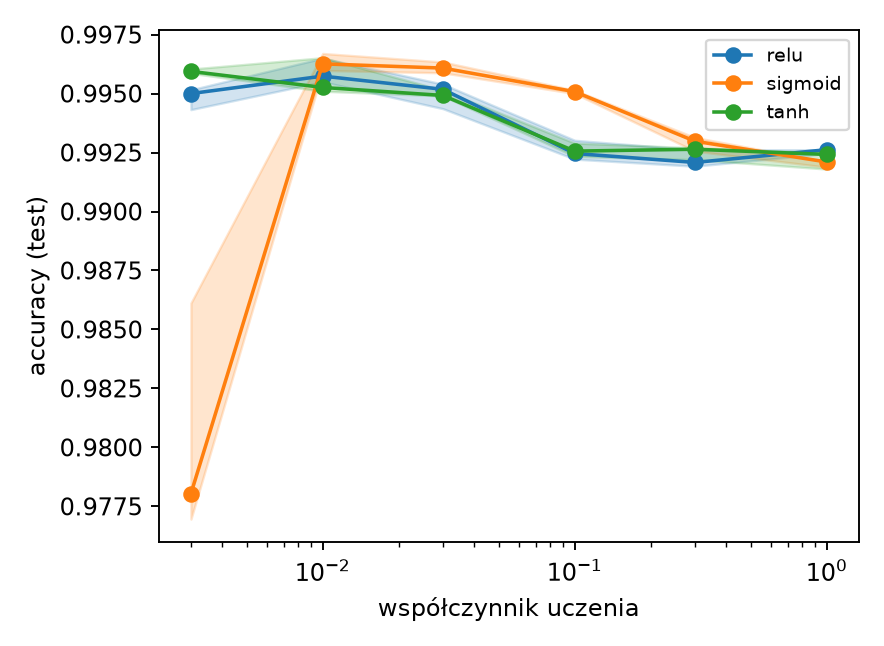
\includegraphics[width=0.7\linewidth]{figures/simple/activation_lr_test_accuracy.png}
  \caption{simple: accuracy (test) dla różnych funkcji aktywacji w zależności od współczynnika uczenia (mediana i kwartyle; liczba przy krzyżyku nad wykresem to liczba rozbieżnych ziaren).}
  \label{fig:simple:activation_lr_test_accuracy}
\end{figure}

\begin{figure}[htbp]
  \centering
  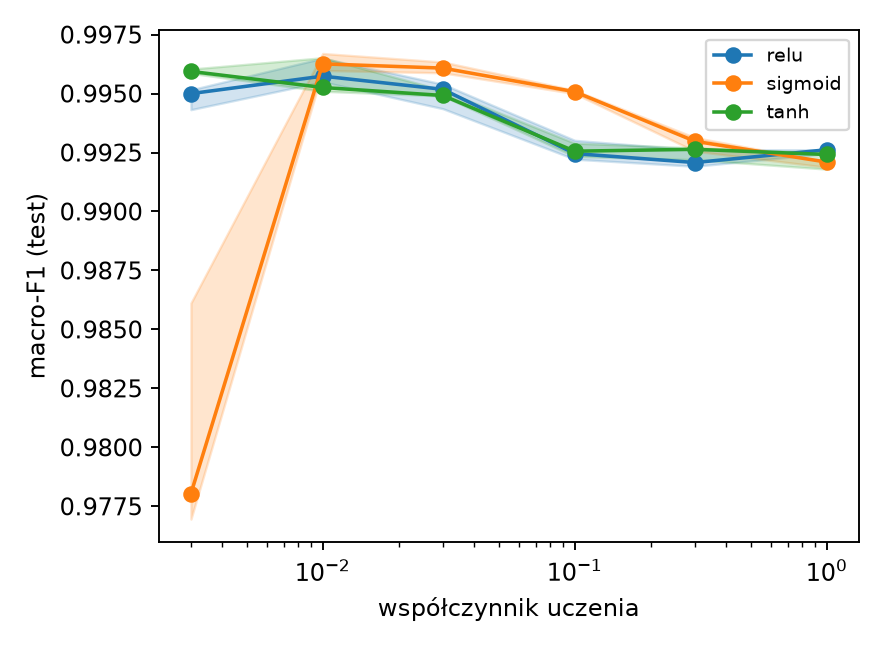
\includegraphics[width=0.7\linewidth]{figures/simple/activation_lr_test_macro_f1.png}
  \caption{simple: macro-F1 (test) dla różnych funkcji aktywacji w zależności od współczynnika uczenia (mediana i kwartyle; liczba przy krzyżyku nad wykresem to liczba rozbieżnych ziaren).}
  \label{fig:simple:activation_lr_test_macro_f1}
\end{figure}

\begin{figure}[htbp]
  \centering
  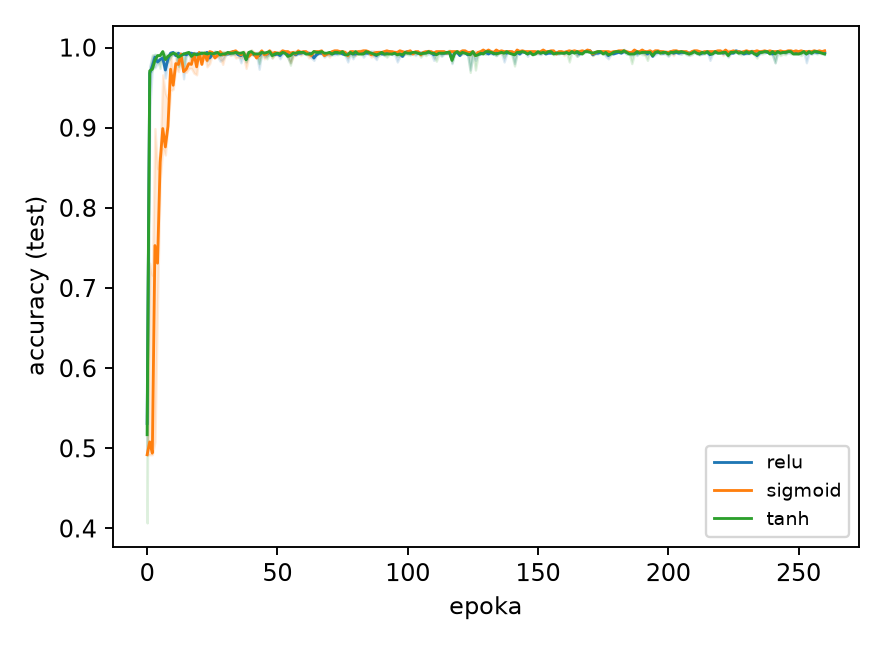
\includegraphics[width=0.7\linewidth]{figures/simple/activation_curve_test_accuracy.png}
  \caption{simple: przebieg accuracy (test) w trakcie uczenia dla różnych funkcji aktywacji (współczynnik uczenia 0.1).}
  \label{fig:simple:activation_curve_test_accuracy}
\end{figure}

\begin{figure}[htbp]
  \centering
  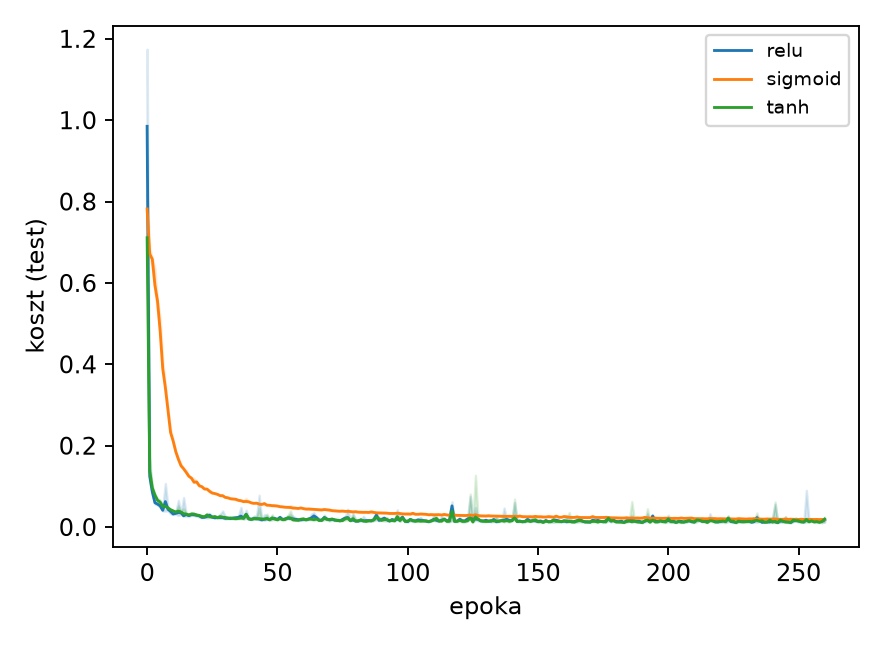
\includegraphics[width=0.7\linewidth]{figures/simple/activation_curve_test_cost.png}
  \caption{simple: przebieg koszt (test) w trakcie uczenia dla różnych funkcji aktywacji (współczynnik uczenia 0.1).}
  \label{fig:simple:activation_curve_test_cost}
\end{figure}

\begin{figure}[htbp]
  \centering
  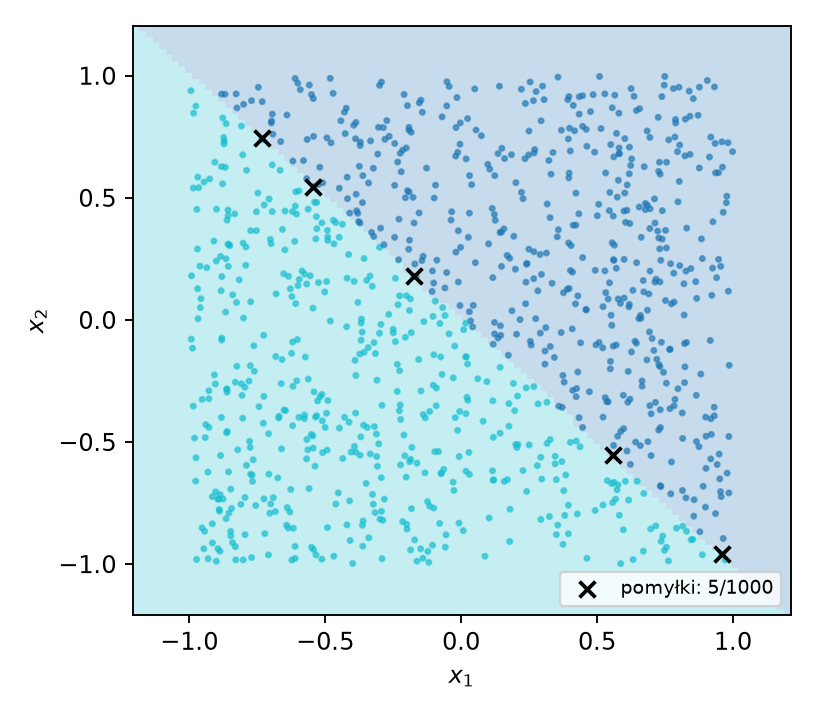
\includegraphics[width=0.7\linewidth]{figures/simple/predictions_relu.png}
  \caption{simple: obszary decyzyjne sieci z aktywacją relu (ziarno 0). Punkty testowe w kolorze prawdziwej klasy, × oznacza pomyłkę (accuracy 0.995).}
  \label{fig:simple:predictions_relu}
\end{figure}

\begin{figure}[htbp]
  \centering
  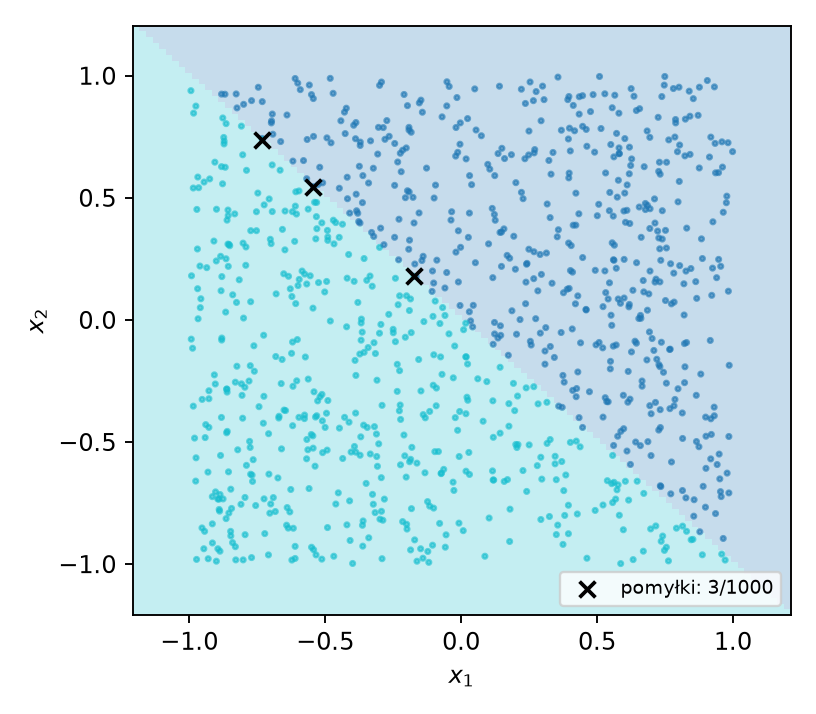
\includegraphics[width=0.7\linewidth]{figures/simple/predictions_sigmoid.png}
  \caption{simple: obszary decyzyjne sieci z aktywacją sigmoid (ziarno 0). Punkty testowe w kolorze prawdziwej klasy, × oznacza pomyłkę (accuracy 0.997).}
  \label{fig:simple:predictions_sigmoid}
\end{figure}

\begin{figure}[htbp]
  \centering
  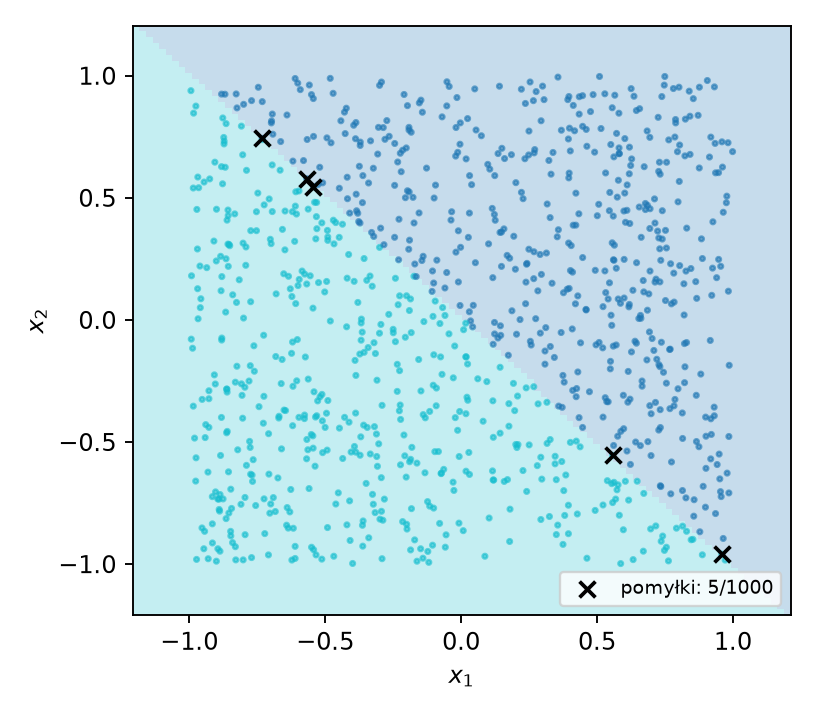
\includegraphics[width=0.7\linewidth]{figures/simple/predictions_tanh.png}
  \caption{simple: obszary decyzyjne sieci z aktywacją tanh (ziarno 0). Punkty testowe w kolorze prawdziwej klasy, × oznacza pomyłkę (accuracy 0.995).}
  \label{fig:simple:predictions_tanh}
\end{figure}

\begin{figure}[htbp]
  \centering
  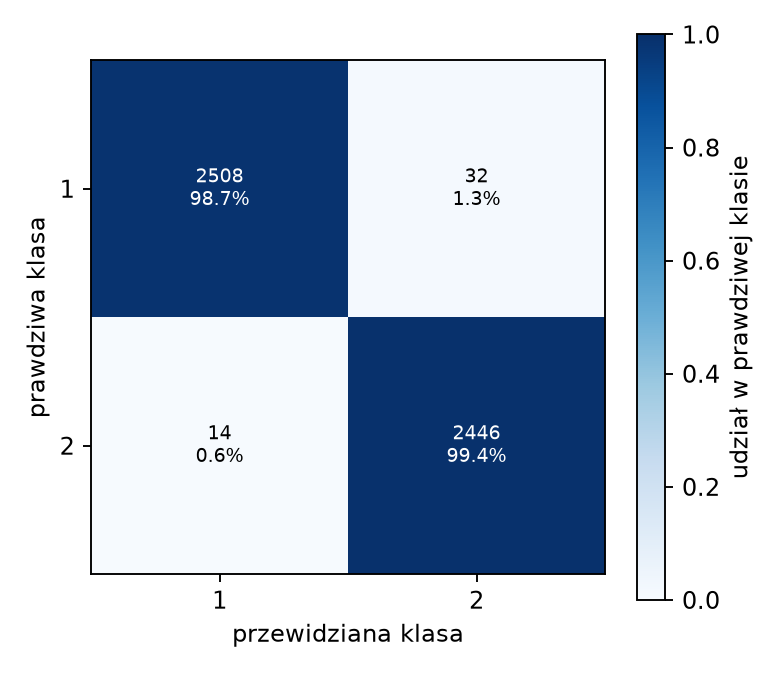
\includegraphics[width=0.7\linewidth]{figures/simple/confusion_relu_32x32.png}
  \caption{simple: macierz pomyłek na zbiorze testowym, aktywacja relu, architektura 32x32, suma po 5 ziarnach (accuracy 0.991).}
  \label{fig:simple:confusion_relu_32x32}
\end{figure}

\begin{figure}[htbp]
  \centering
  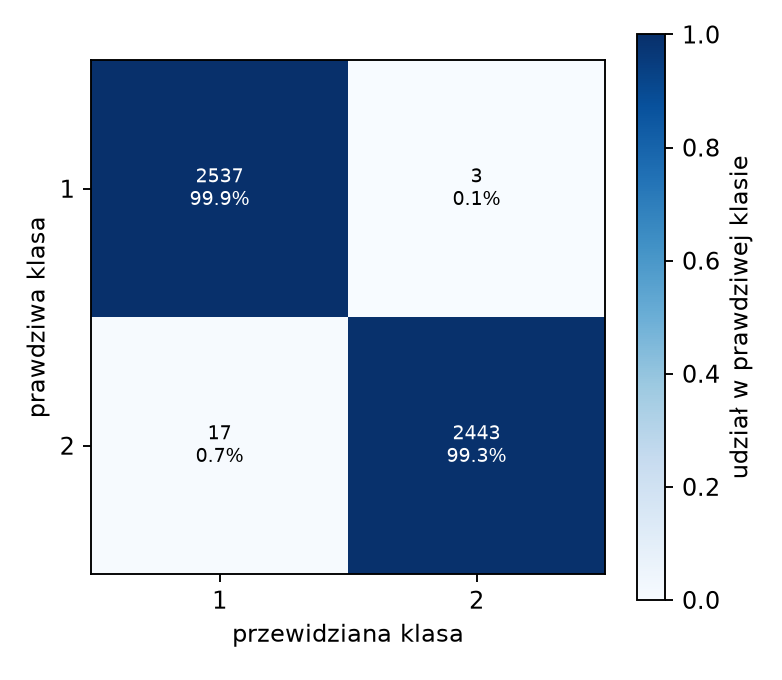
\includegraphics[width=0.7\linewidth]{figures/simple/confusion_sigmoid_32x32.png}
  \caption{simple: macierz pomyłek na zbiorze testowym, aktywacja sigmoid, architektura 32x32, suma po 5 ziarnach (accuracy 0.996).}
  \label{fig:simple:confusion_sigmoid_32x32}
\end{figure}

\begin{figure}[htbp]
  \centering
  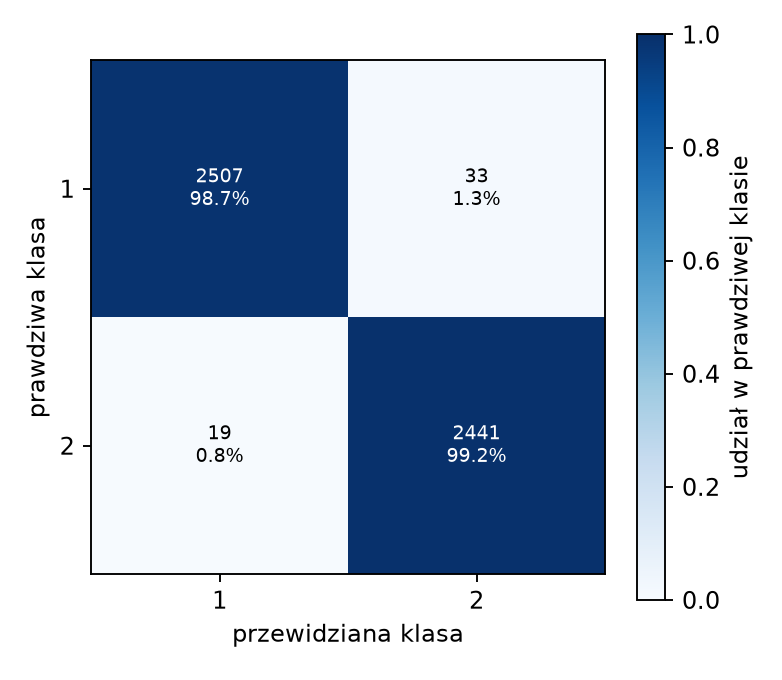
\includegraphics[width=0.7\linewidth]{figures/simple/confusion_tanh_32x32.png}
  \caption{simple: macierz pomyłek na zbiorze testowym, aktywacja tanh, architektura 32x32, suma po 5 ziarnach (accuracy 0.990).}
  \label{fig:simple:confusion_tanh_32x32}
\end{figure}

\begin{figure}[htbp]
  \centering
  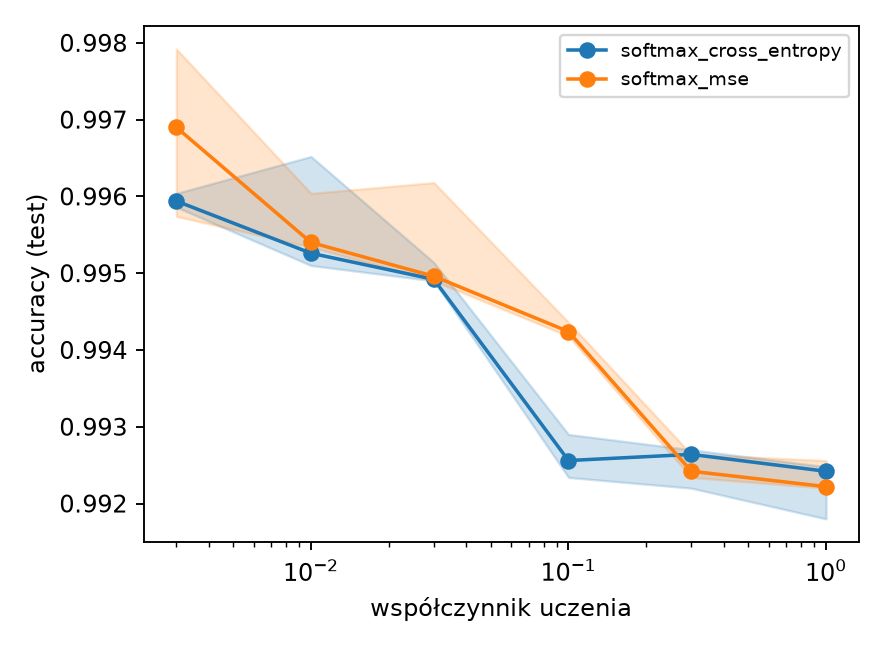
\includegraphics[width=0.7\linewidth]{figures/simple/loss_lr_test_accuracy.png}
  \caption{simple: accuracy (test) dla różnych funkcji kosztu w zależności od współczynnika uczenia (mediana i kwartyle; liczba przy krzyżyku nad wykresem to liczba rozbieżnych ziaren).}
  \label{fig:simple:loss_lr_test_accuracy}
\end{figure}

\begin{figure}[htbp]
  \centering
  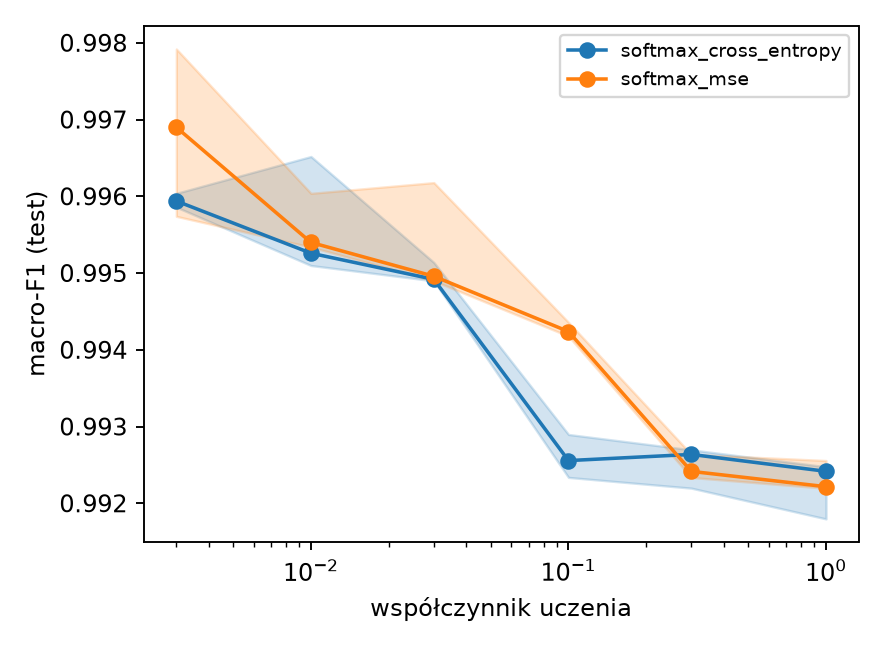
\includegraphics[width=0.7\linewidth]{figures/simple/loss_lr_test_macro_f1.png}
  \caption{simple: macro-F1 (test) dla różnych funkcji kosztu w zależności od współczynnika uczenia (mediana i kwartyle; liczba przy krzyżyku nad wykresem to liczba rozbieżnych ziaren).}
  \label{fig:simple:loss_lr_test_macro_f1}
\end{figure}

\begin{figure}[htbp]
  \centering
  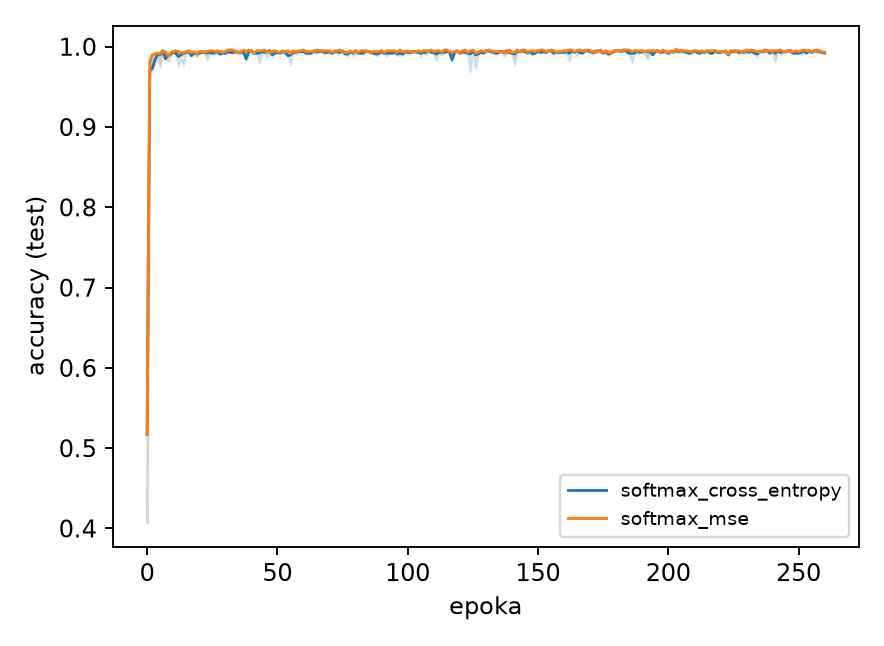
\includegraphics[width=0.7\linewidth]{figures/simple/loss_curve_test_accuracy.png}
  \caption{simple: przebieg accuracy (test) w trakcie uczenia dla różnych funkcji kosztu (współczynnik uczenia 0.1).}
  \label{fig:simple:loss_curve_test_accuracy}
\end{figure}

\begin{figure}[htbp]
  \centering
  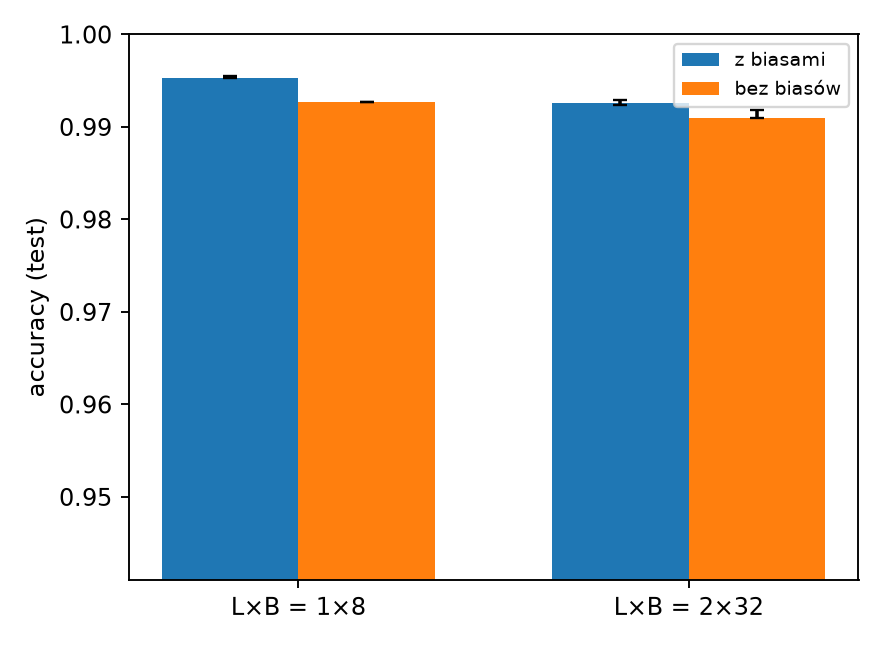
\includegraphics[width=0.7\linewidth]{figures/simple/bias.png}
  \caption{simple: accuracy (test) sieci z biasami i bez biasów.}
  \label{fig:simple:bias}
\end{figure}

\begin{figure}[htbp]
  \centering
  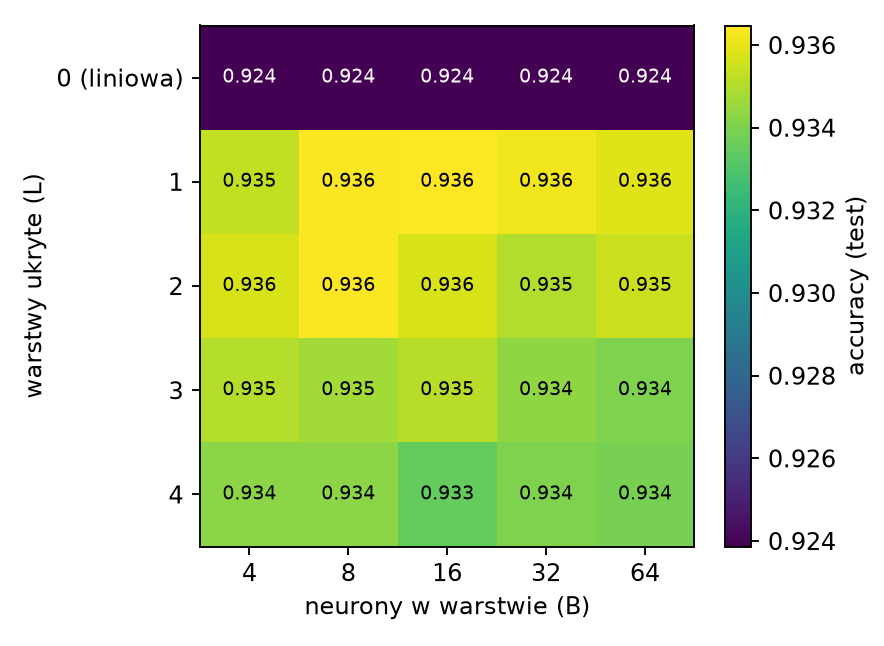
\includegraphics[width=0.7\linewidth]{figures/three_gauss/arch_heatmap_test_accuracy.png}
  \caption{three\_gauss: accuracy (test) (mediana) w zależności od liczby warstw ukrytych $L$ i neuronów w warstwie $B$.}
  \label{fig:three_gauss:arch_heatmap_test_accuracy}
\end{figure}

\begin{figure}[htbp]
  \centering
  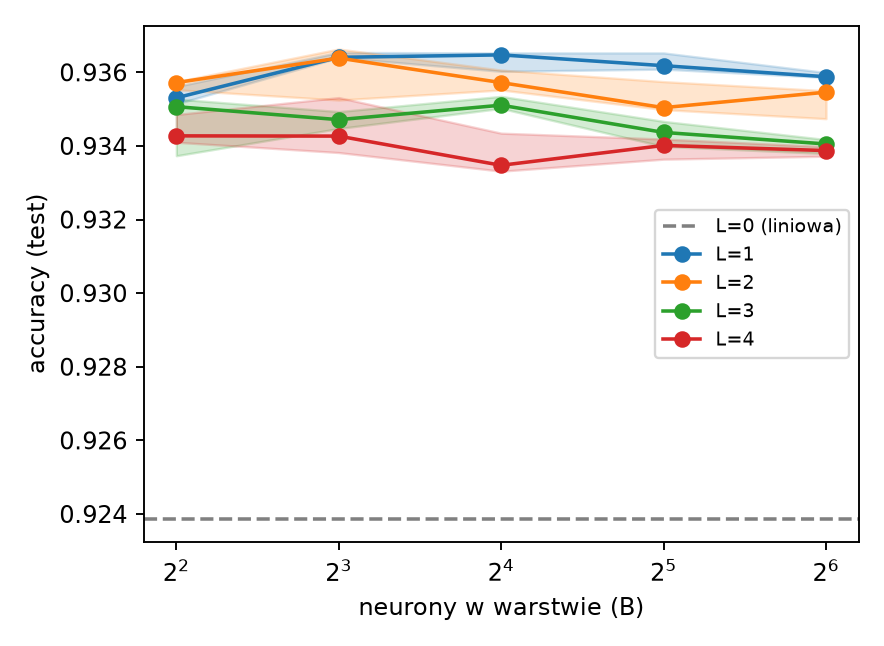
\includegraphics[width=0.7\linewidth]{figures/three_gauss/arch_lines_test_accuracy.png}
  \caption{three\_gauss: accuracy (test) w zależności od $B$ dla każdej liczby warstw $L$ (mediana i kwartyle po ziarnach).}
  \label{fig:three_gauss:arch_lines_test_accuracy}
\end{figure}

\begin{figure}[htbp]
  \centering
  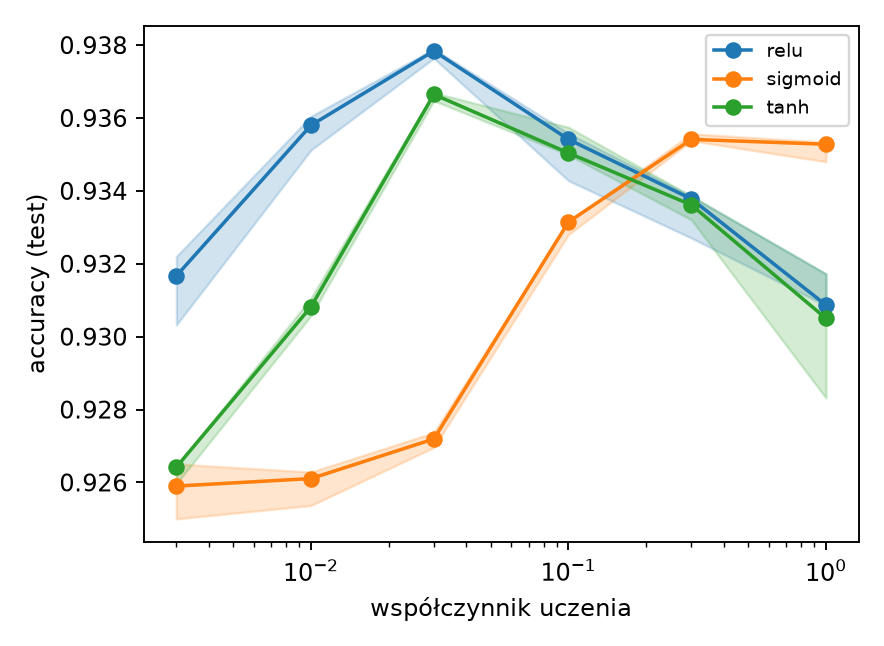
\includegraphics[width=0.7\linewidth]{figures/three_gauss/activation_lr_test_accuracy.png}
  \caption{three\_gauss: accuracy (test) dla różnych funkcji aktywacji w zależności od współczynnika uczenia (mediana i kwartyle; liczba przy krzyżyku nad wykresem to liczba rozbieżnych ziaren).}
  \label{fig:three_gauss:activation_lr_test_accuracy}
\end{figure}

\begin{figure}[htbp]
  \centering
  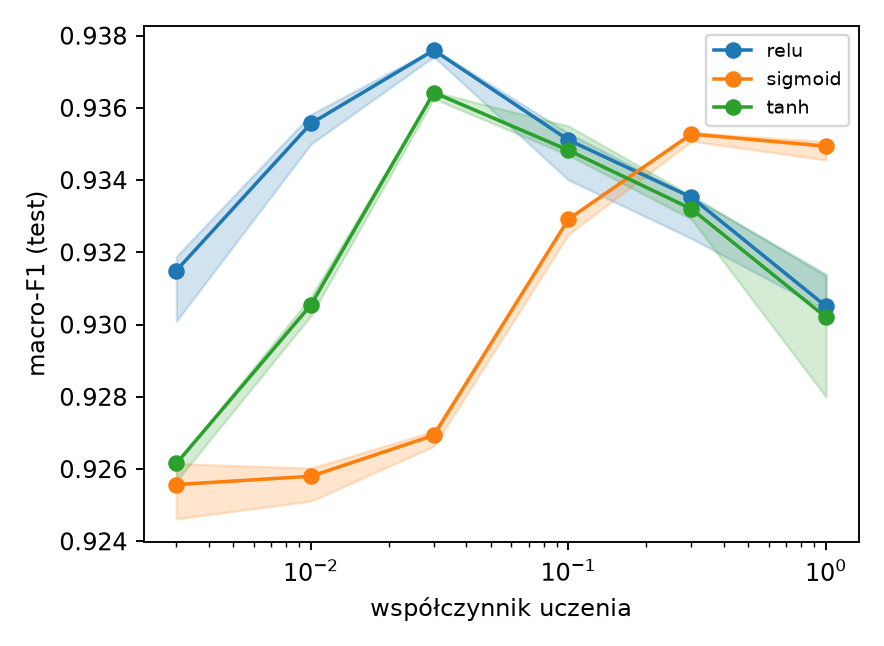
\includegraphics[width=0.7\linewidth]{figures/three_gauss/activation_lr_test_macro_f1.png}
  \caption{three\_gauss: macro-F1 (test) dla różnych funkcji aktywacji w zależności od współczynnika uczenia (mediana i kwartyle; liczba przy krzyżyku nad wykresem to liczba rozbieżnych ziaren).}
  \label{fig:three_gauss:activation_lr_test_macro_f1}
\end{figure}

\begin{figure}[htbp]
  \centering
  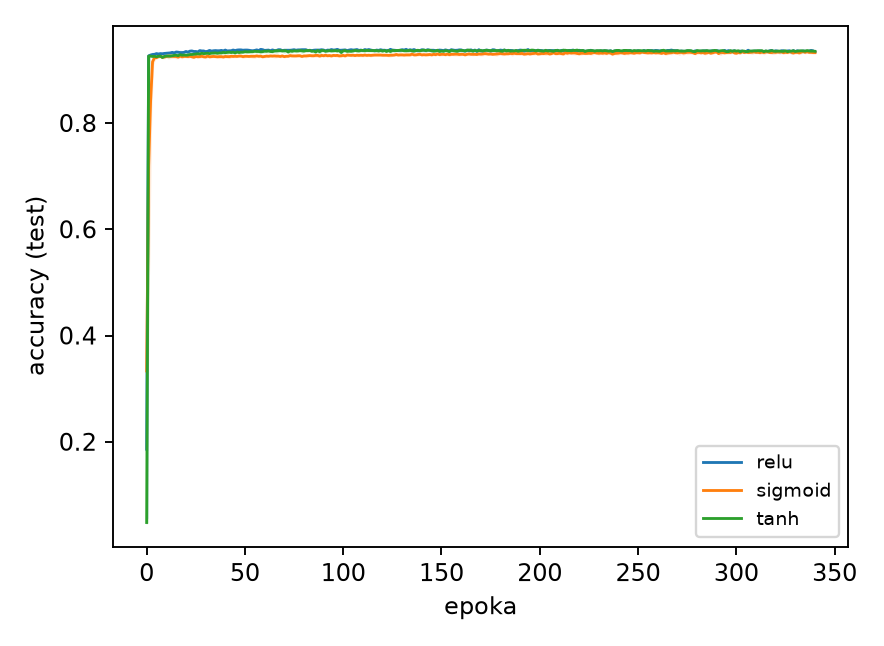
\includegraphics[width=0.7\linewidth]{figures/three_gauss/activation_curve_test_accuracy.png}
  \caption{three\_gauss: przebieg accuracy (test) w trakcie uczenia dla różnych funkcji aktywacji (współczynnik uczenia 0.1).}
  \label{fig:three_gauss:activation_curve_test_accuracy}
\end{figure}

\begin{figure}[htbp]
  \centering
  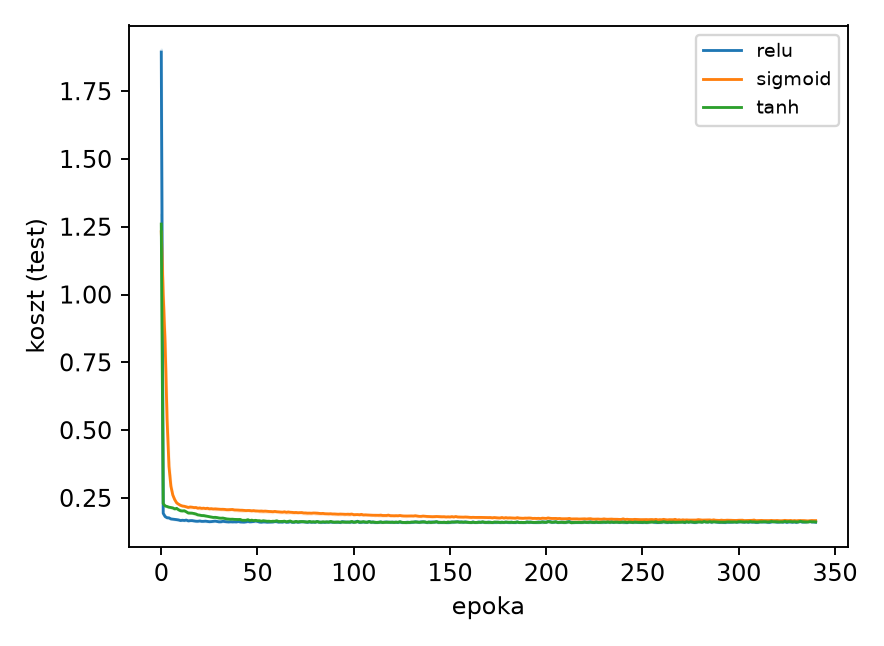
\includegraphics[width=0.7\linewidth]{figures/three_gauss/activation_curve_test_cost.png}
  \caption{three\_gauss: przebieg koszt (test) w trakcie uczenia dla różnych funkcji aktywacji (współczynnik uczenia 0.1).}
  \label{fig:three_gauss:activation_curve_test_cost}
\end{figure}

\begin{figure}[htbp]
  \centering
  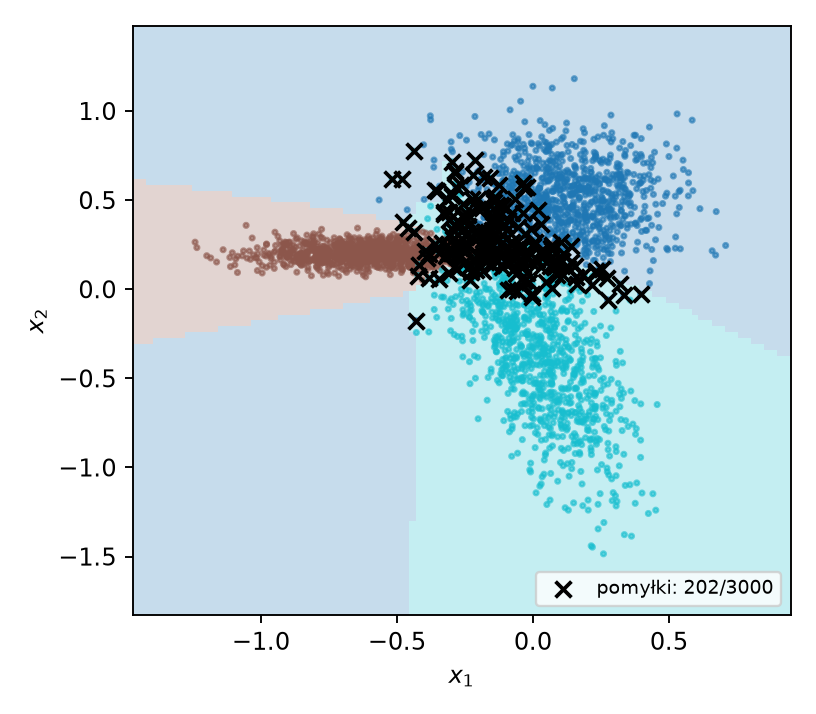
\includegraphics[width=0.7\linewidth]{figures/three_gauss/predictions_relu.png}
  \caption{three\_gauss: obszary decyzyjne sieci z aktywacją relu (ziarno 0). Punkty testowe w kolorze prawdziwej klasy, × oznacza pomyłkę (accuracy 0.933).}
  \label{fig:three_gauss:predictions_relu}
\end{figure}

\begin{figure}[htbp]
  \centering
  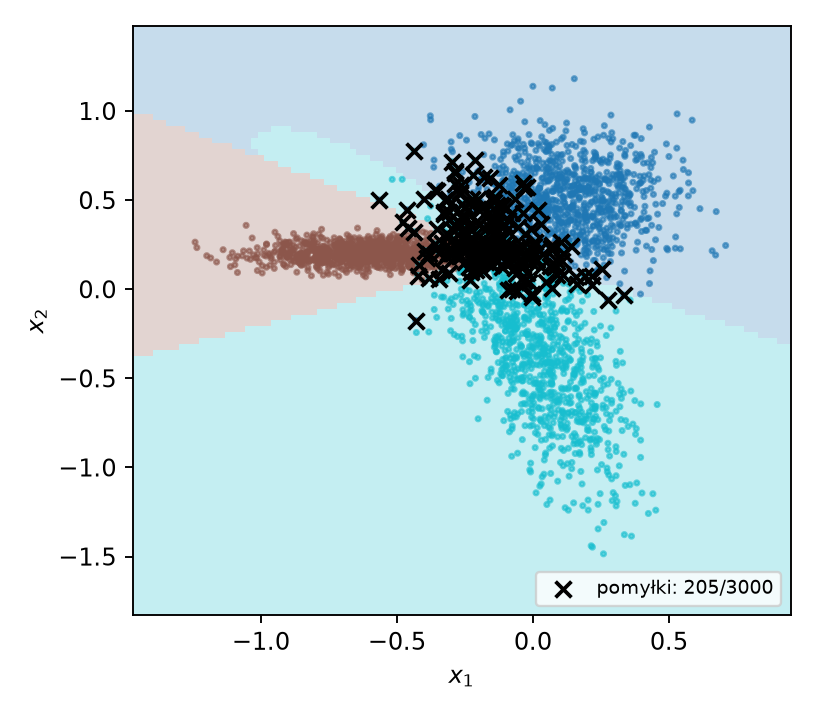
\includegraphics[width=0.7\linewidth]{figures/three_gauss/predictions_sigmoid.png}
  \caption{three\_gauss: obszary decyzyjne sieci z aktywacją sigmoid (ziarno 0). Punkty testowe w kolorze prawdziwej klasy, × oznacza pomyłkę (accuracy 0.932).}
  \label{fig:three_gauss:predictions_sigmoid}
\end{figure}

\begin{figure}[htbp]
  \centering
  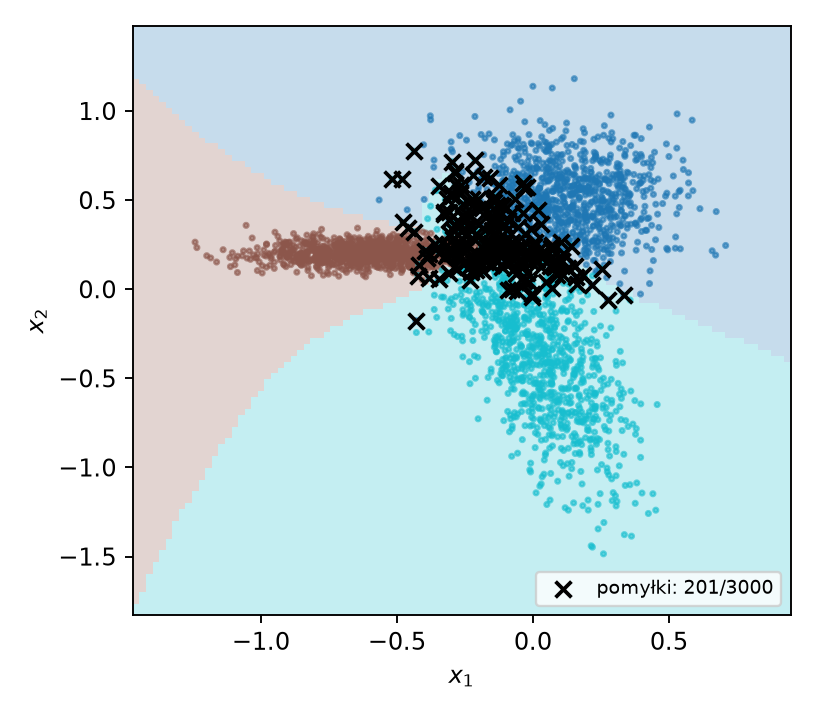
\includegraphics[width=0.7\linewidth]{figures/three_gauss/predictions_tanh.png}
  \caption{three\_gauss: obszary decyzyjne sieci z aktywacją tanh (ziarno 0). Punkty testowe w kolorze prawdziwej klasy, × oznacza pomyłkę (accuracy 0.933).}
  \label{fig:three_gauss:predictions_tanh}
\end{figure}

\begin{figure}[htbp]
  \centering
  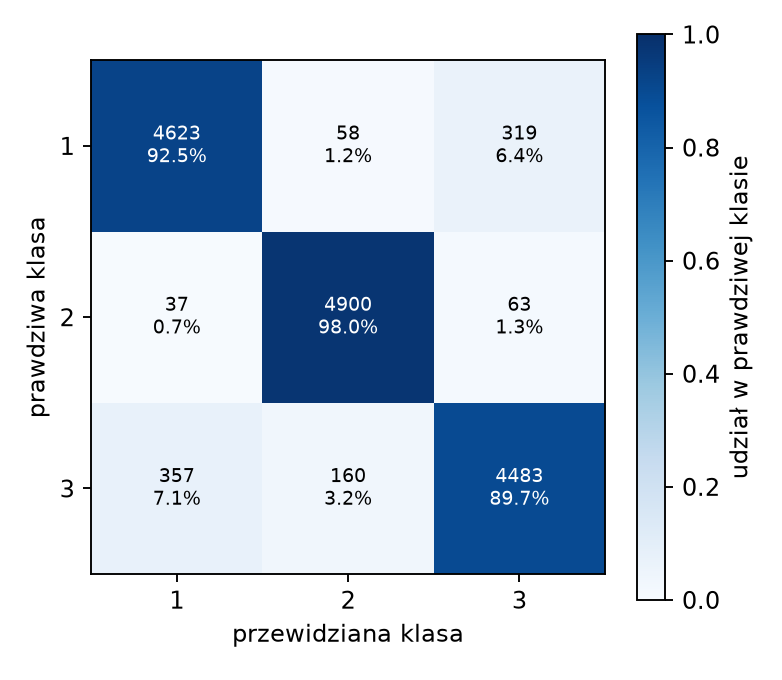
\includegraphics[width=0.7\linewidth]{figures/three_gauss/confusion_relu_32x32.png}
  \caption{three\_gauss: macierz pomyłek na zbiorze testowym, aktywacja relu, architektura 32x32, suma po 5 ziarnach (accuracy 0.934).}
  \label{fig:three_gauss:confusion_relu_32x32}
\end{figure}

\begin{figure}[htbp]
  \centering
  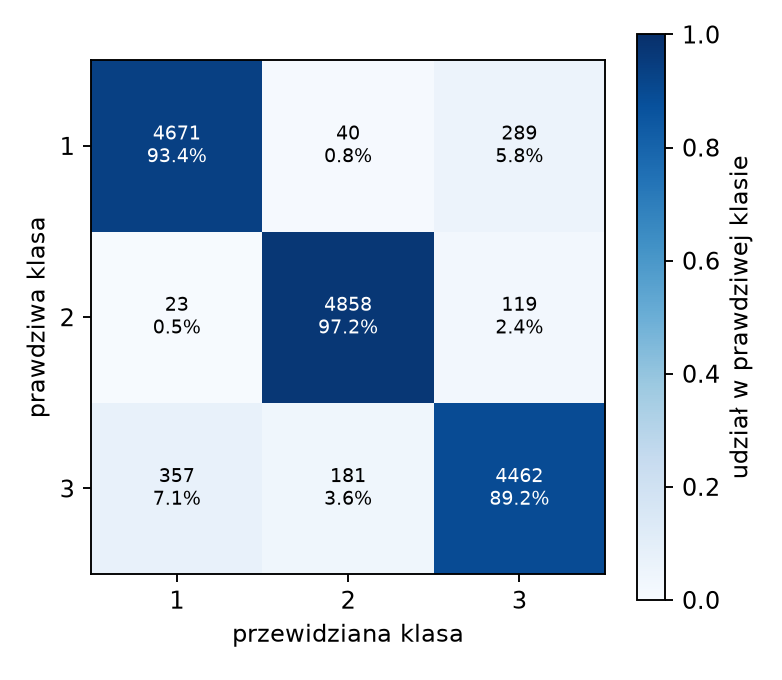
\includegraphics[width=0.7\linewidth]{figures/three_gauss/confusion_sigmoid_32x32.png}
  \caption{three\_gauss: macierz pomyłek na zbiorze testowym, aktywacja sigmoid, architektura 32x32, suma po 5 ziarnach (accuracy 0.933).}
  \label{fig:three_gauss:confusion_sigmoid_32x32}
\end{figure}

\begin{figure}[htbp]
  \centering
  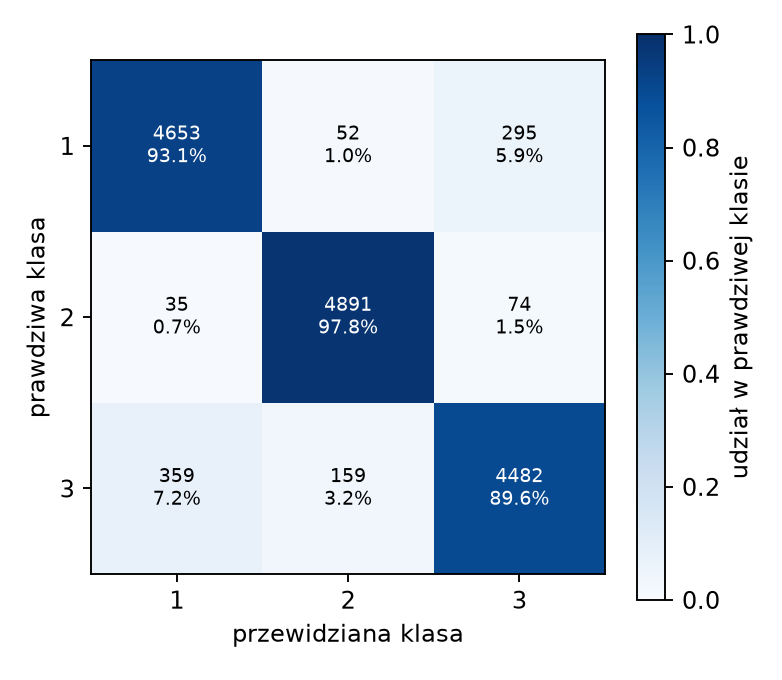
\includegraphics[width=0.7\linewidth]{figures/three_gauss/confusion_tanh_32x32.png}
  \caption{three\_gauss: macierz pomyłek na zbiorze testowym, aktywacja tanh, architektura 32x32, suma po 5 ziarnach (accuracy 0.935).}
  \label{fig:three_gauss:confusion_tanh_32x32}
\end{figure}

\begin{figure}[htbp]
  \centering
  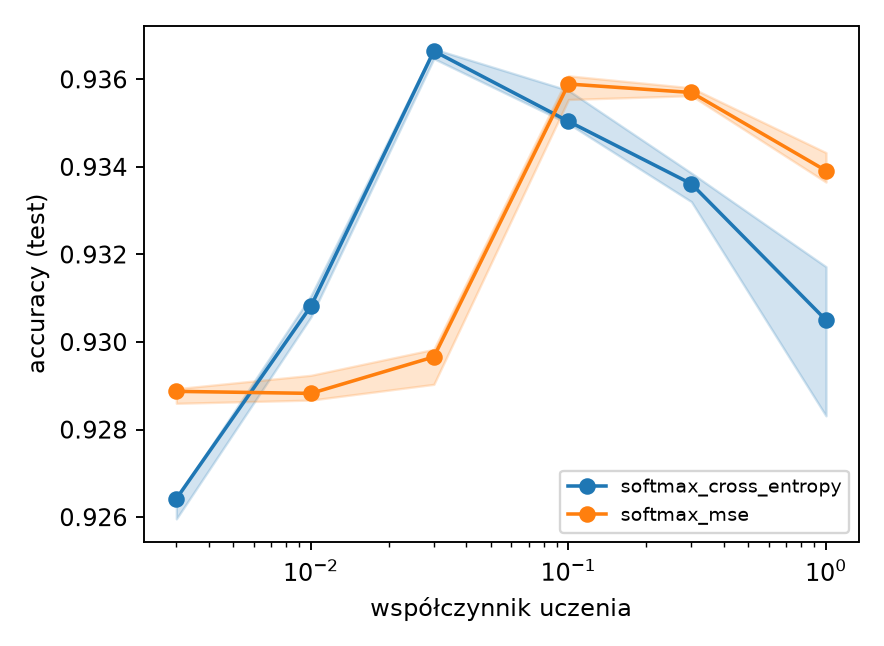
\includegraphics[width=0.7\linewidth]{figures/three_gauss/loss_lr_test_accuracy.png}
  \caption{three\_gauss: accuracy (test) dla różnych funkcji kosztu w zależności od współczynnika uczenia (mediana i kwartyle; liczba przy krzyżyku nad wykresem to liczba rozbieżnych ziaren).}
  \label{fig:three_gauss:loss_lr_test_accuracy}
\end{figure}

\begin{figure}[htbp]
  \centering
  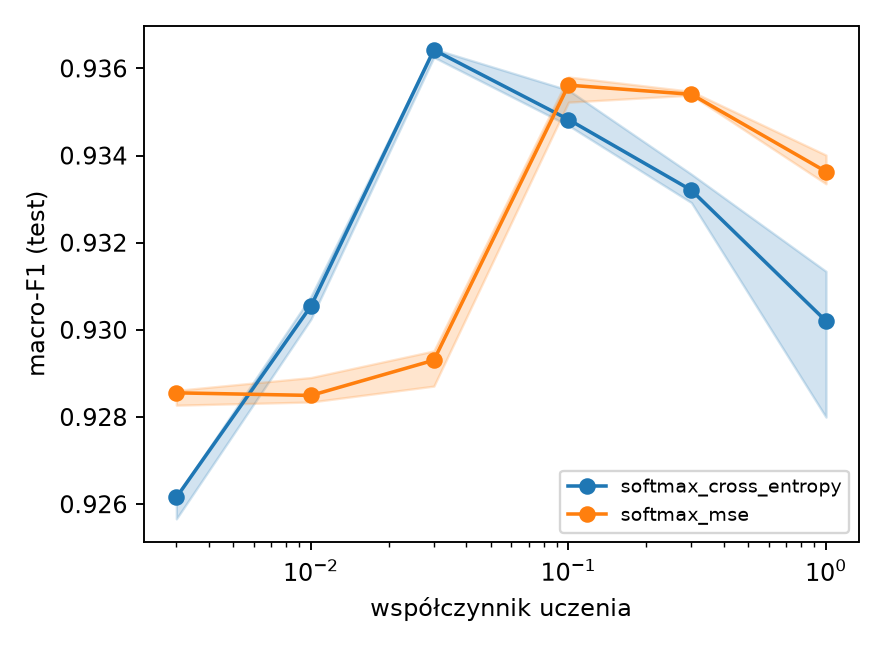
\includegraphics[width=0.7\linewidth]{figures/three_gauss/loss_lr_test_macro_f1.png}
  \caption{three\_gauss: macro-F1 (test) dla różnych funkcji kosztu w zależności od współczynnika uczenia (mediana i kwartyle; liczba przy krzyżyku nad wykresem to liczba rozbieżnych ziaren).}
  \label{fig:three_gauss:loss_lr_test_macro_f1}
\end{figure}

\begin{figure}[htbp]
  \centering
  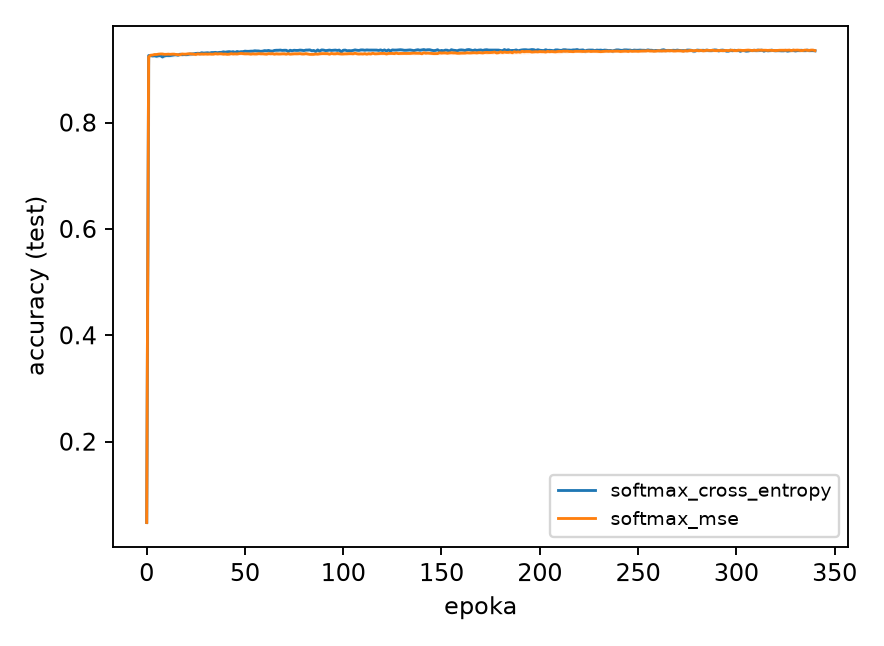
\includegraphics[width=0.7\linewidth]{figures/three_gauss/loss_curve_test_accuracy.png}
  \caption{three\_gauss: przebieg accuracy (test) w trakcie uczenia dla różnych funkcji kosztu (współczynnik uczenia 0.1).}
  \label{fig:three_gauss:loss_curve_test_accuracy}
\end{figure}

\begin{figure}[htbp]
  \centering
  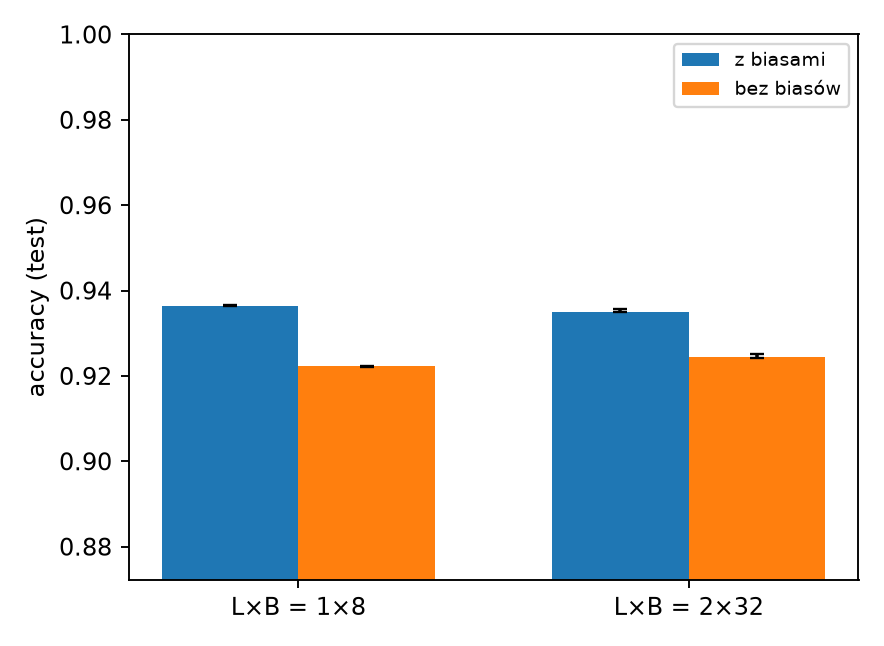
\includegraphics[width=0.7\linewidth]{figures/three_gauss/bias.png}
  \caption{three\_gauss: accuracy (test) sieci z biasami i bez biasów.}
  \label{fig:three_gauss:bias}
\end{figure}

\begin{figure}[htbp]
  \centering
  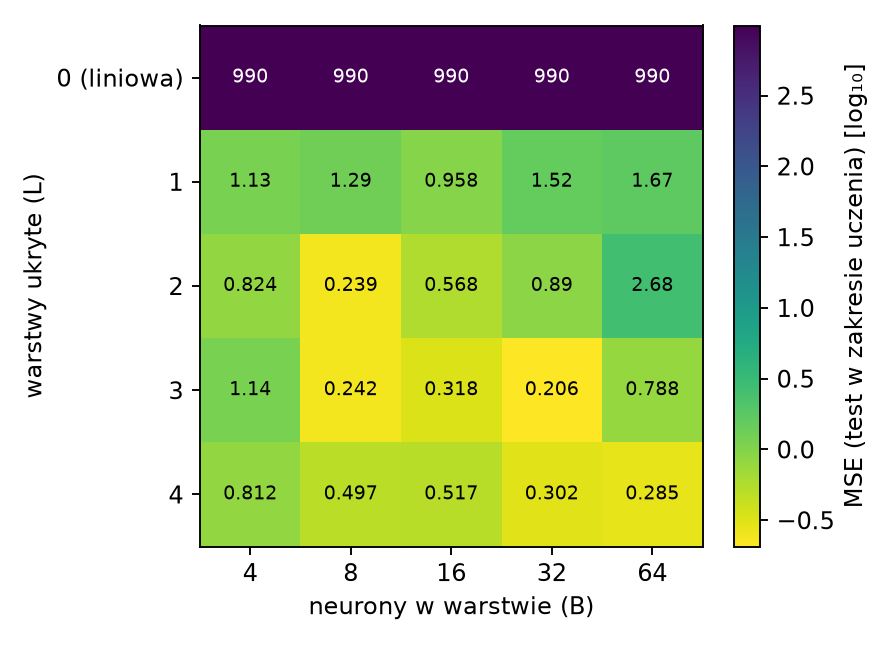
\includegraphics[width=0.7\linewidth]{figures/cube/arch_heatmap_test_in_mse.png}
  \caption{cube: MSE (test w zakresie uczenia) (mediana) w zależności od liczby warstw ukrytych $L$ i neuronów w warstwie $B$.}
  \label{fig:cube:arch_heatmap_test_in_mse}
\end{figure}

\begin{figure}[htbp]
  \centering
  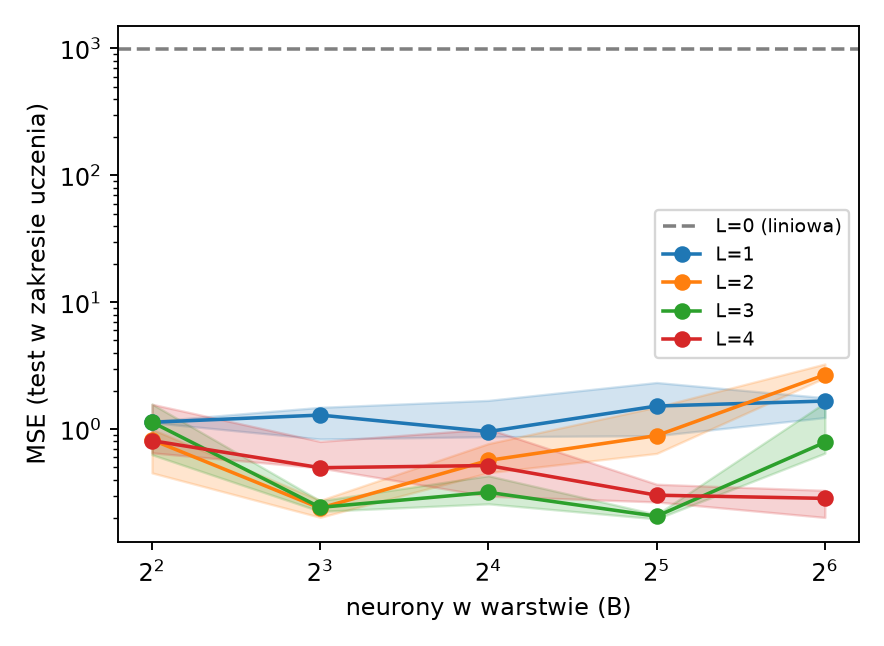
\includegraphics[width=0.7\linewidth]{figures/cube/arch_lines_test_in_mse.png}
  \caption{cube: MSE (test w zakresie uczenia) w zależności od $B$ dla każdej liczby warstw $L$ (mediana i kwartyle po ziarnach).}
  \label{fig:cube:arch_lines_test_in_mse}
\end{figure}

\begin{figure}[htbp]
  \centering
  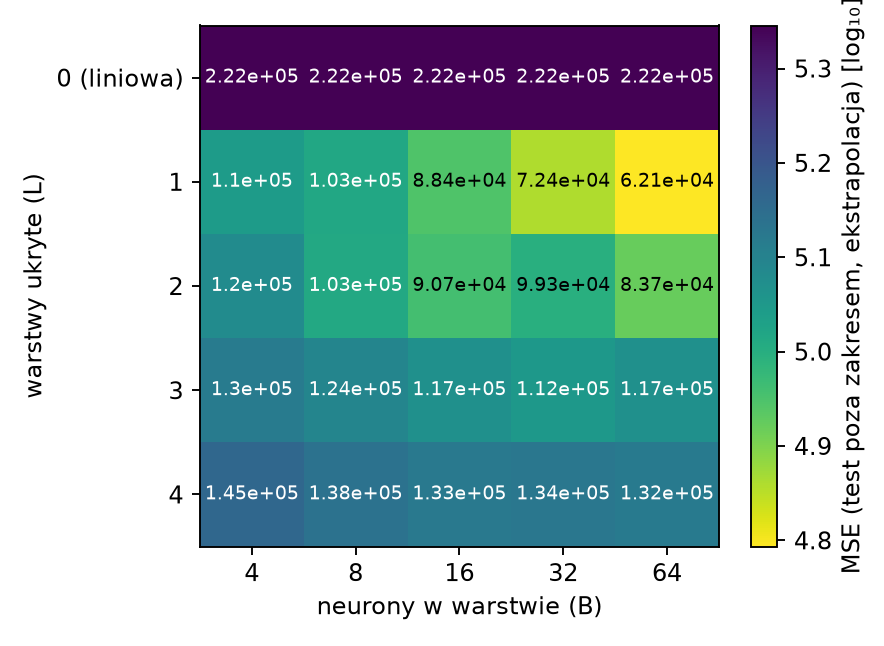
\includegraphics[width=0.7\linewidth]{figures/cube/arch_heatmap_test_out_mse.png}
  \caption{cube: MSE (test poza zakresem, ekstrapolacja) (mediana) w zależności od liczby warstw ukrytych $L$ i neuronów w warstwie $B$.}
  \label{fig:cube:arch_heatmap_test_out_mse}
\end{figure}

\begin{figure}[htbp]
  \centering
  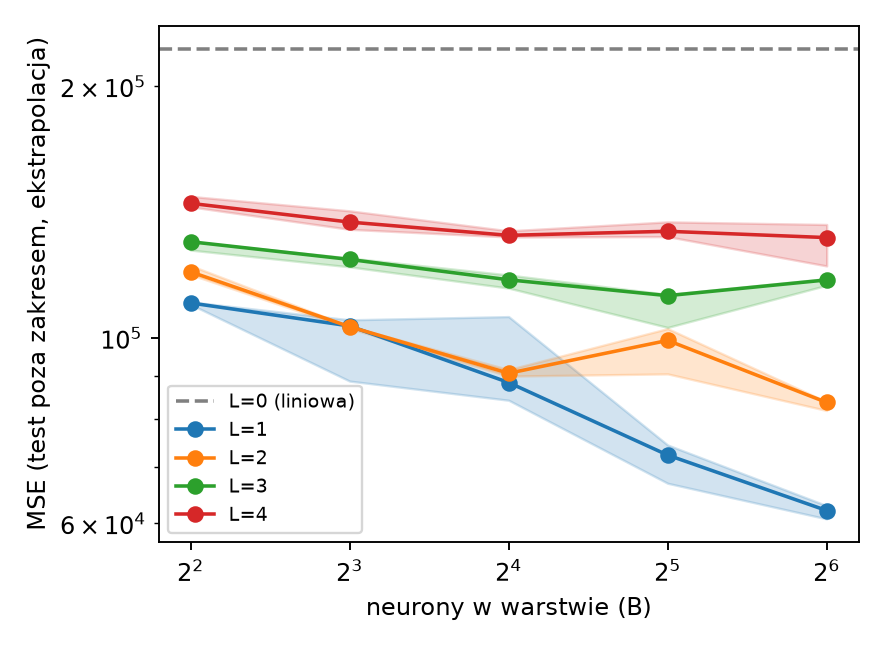
\includegraphics[width=0.7\linewidth]{figures/cube/arch_lines_test_out_mse.png}
  \caption{cube: MSE (test poza zakresem, ekstrapolacja) w zależności od $B$ dla każdej liczby warstw $L$ (mediana i kwartyle po ziarnach).}
  \label{fig:cube:arch_lines_test_out_mse}
\end{figure}

\begin{figure}[htbp]
  \centering
  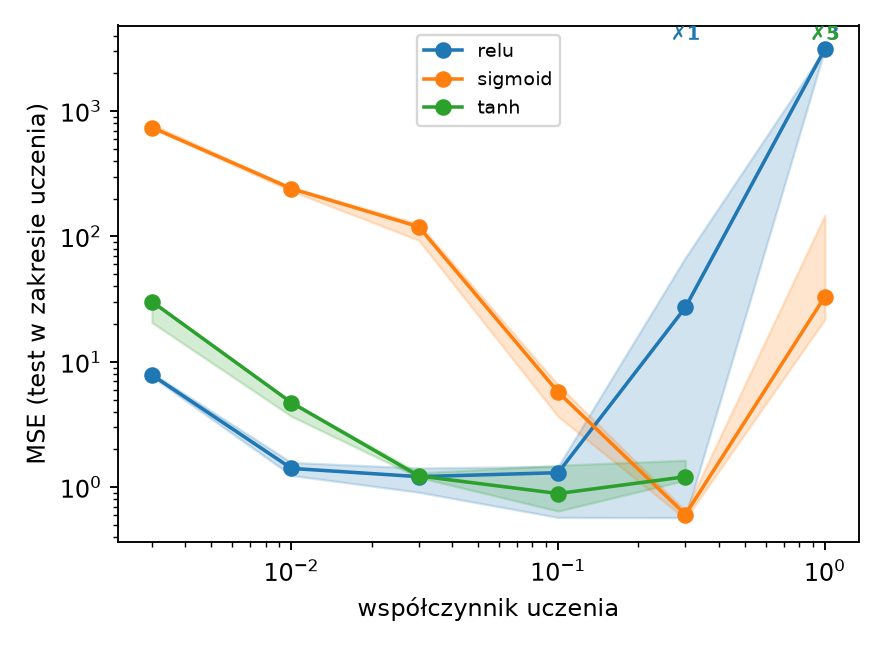
\includegraphics[width=0.7\linewidth]{figures/cube/activation_lr_test_in_mse.png}
  \caption{cube: MSE (test w zakresie uczenia) dla różnych funkcji aktywacji w zależności od współczynnika uczenia (mediana i kwartyle; liczba przy krzyżyku nad wykresem to liczba rozbieżnych ziaren).}
  \label{fig:cube:activation_lr_test_in_mse}
\end{figure}

\begin{figure}[htbp]
  \centering
  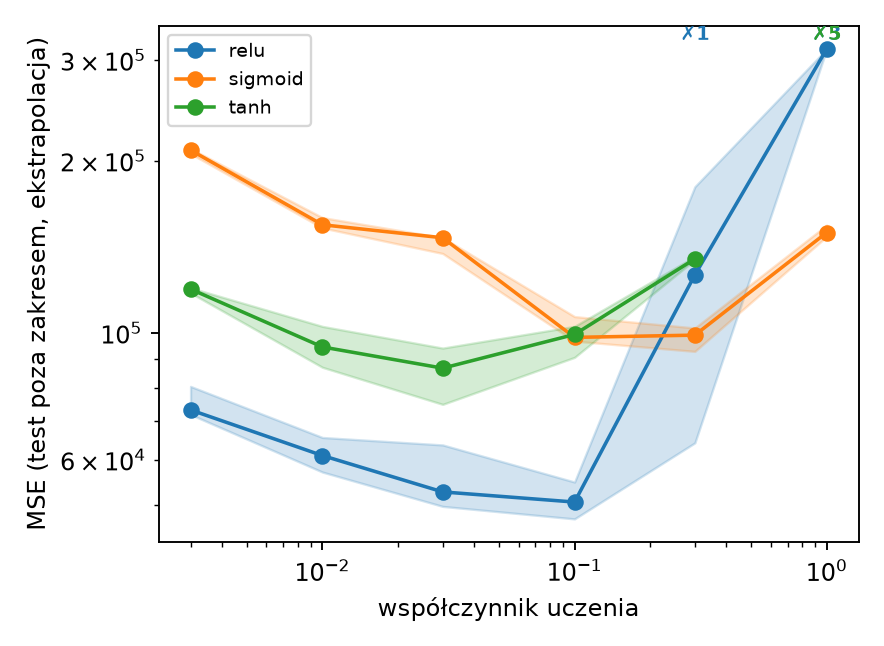
\includegraphics[width=0.7\linewidth]{figures/cube/activation_lr_test_out_mse.png}
  \caption{cube: MSE (test poza zakresem, ekstrapolacja) dla różnych funkcji aktywacji w zależności od współczynnika uczenia (mediana i kwartyle; liczba przy krzyżyku nad wykresem to liczba rozbieżnych ziaren).}
  \label{fig:cube:activation_lr_test_out_mse}
\end{figure}

\begin{figure}[htbp]
  \centering
  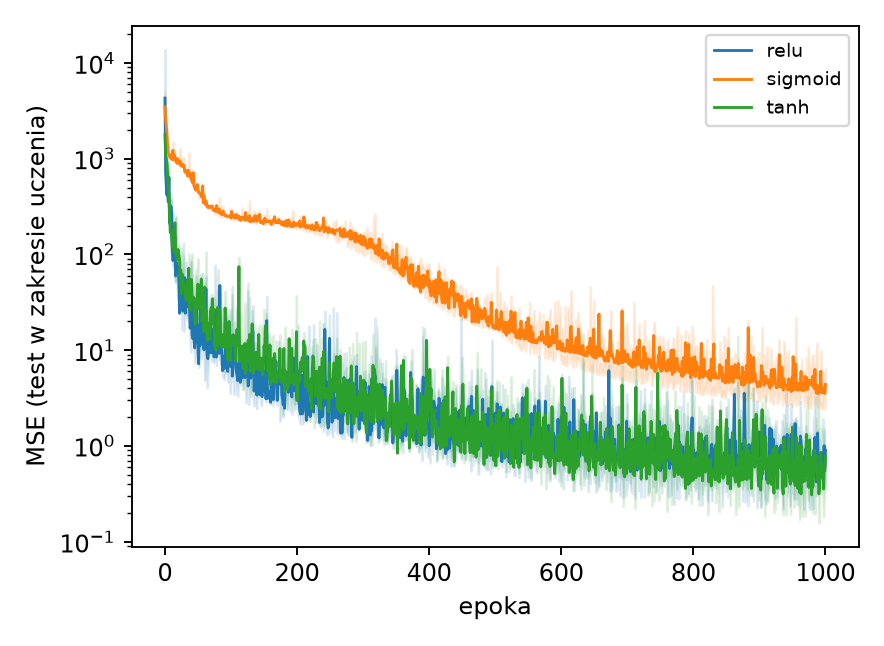
\includegraphics[width=0.7\linewidth]{figures/cube/activation_curve_test_in_mse.png}
  \caption{cube: przebieg MSE (test w zakresie uczenia) w trakcie uczenia dla różnych funkcji aktywacji (współczynnik uczenia 0.1).}
  \label{fig:cube:activation_curve_test_in_mse}
\end{figure}

\begin{figure}[htbp]
  \centering
  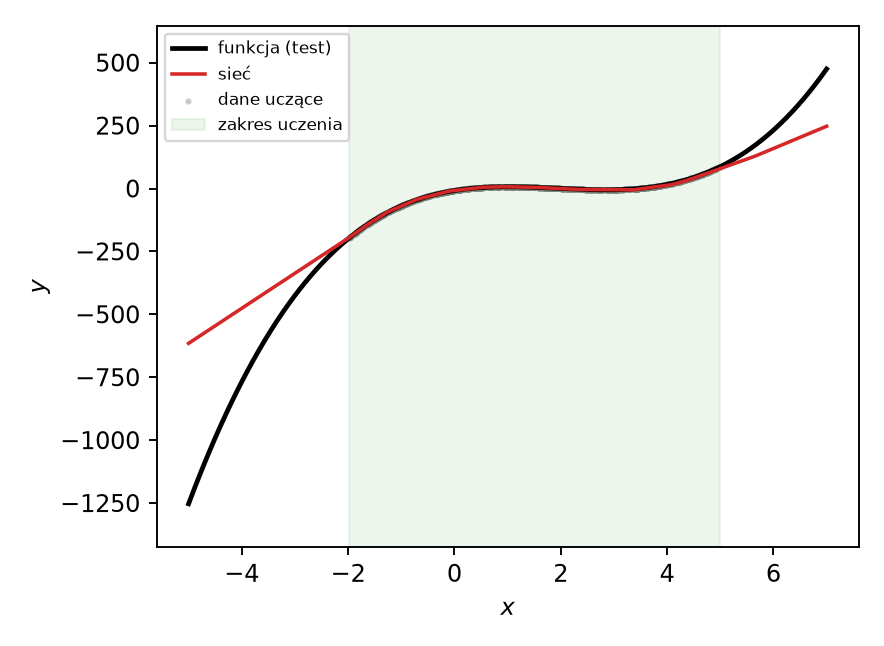
\includegraphics[width=0.7\linewidth]{figures/cube/predictions_relu.png}
  \caption{cube: funkcja nauczona przez sieć z aktywacją relu (ziarno 0) na całym zakresie testu; zielone tło to zakres danych uczących.}
  \label{fig:cube:predictions_relu}
\end{figure}

\begin{figure}[htbp]
  \centering
  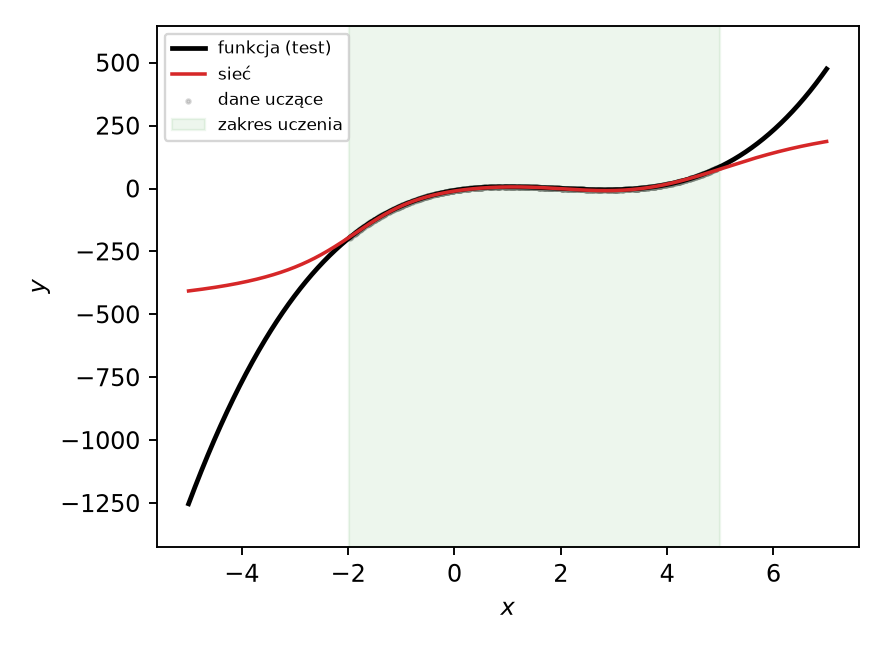
\includegraphics[width=0.7\linewidth]{figures/cube/predictions_sigmoid.png}
  \caption{cube: funkcja nauczona przez sieć z aktywacją sigmoid (ziarno 0) na całym zakresie testu; zielone tło to zakres danych uczących.}
  \label{fig:cube:predictions_sigmoid}
\end{figure}

\begin{figure}[htbp]
  \centering
  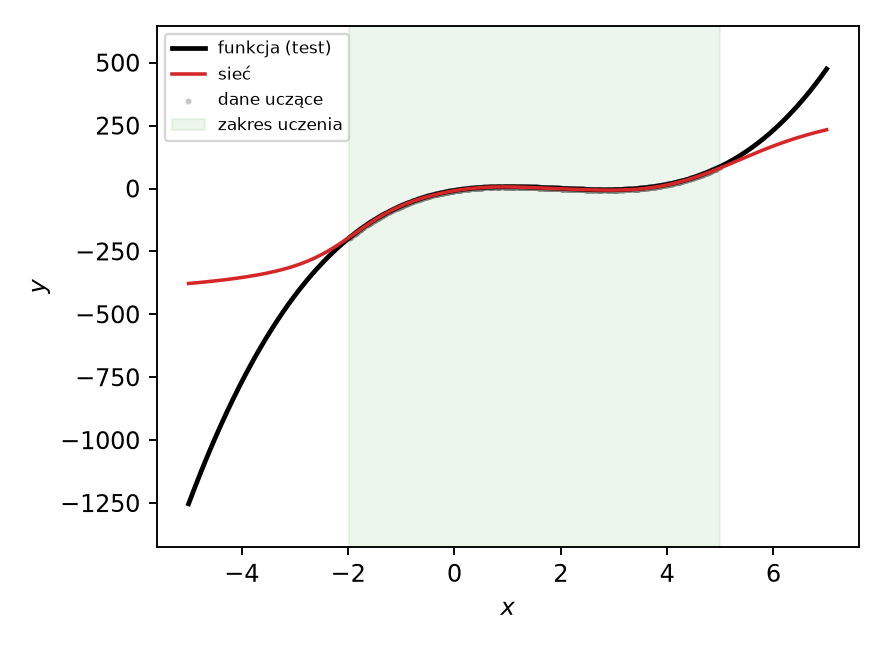
\includegraphics[width=0.7\linewidth]{figures/cube/predictions_tanh.png}
  \caption{cube: funkcja nauczona przez sieć z aktywacją tanh (ziarno 0) na całym zakresie testu; zielone tło to zakres danych uczących.}
  \label{fig:cube:predictions_tanh}
\end{figure}

\begin{figure}[htbp]
  \centering
  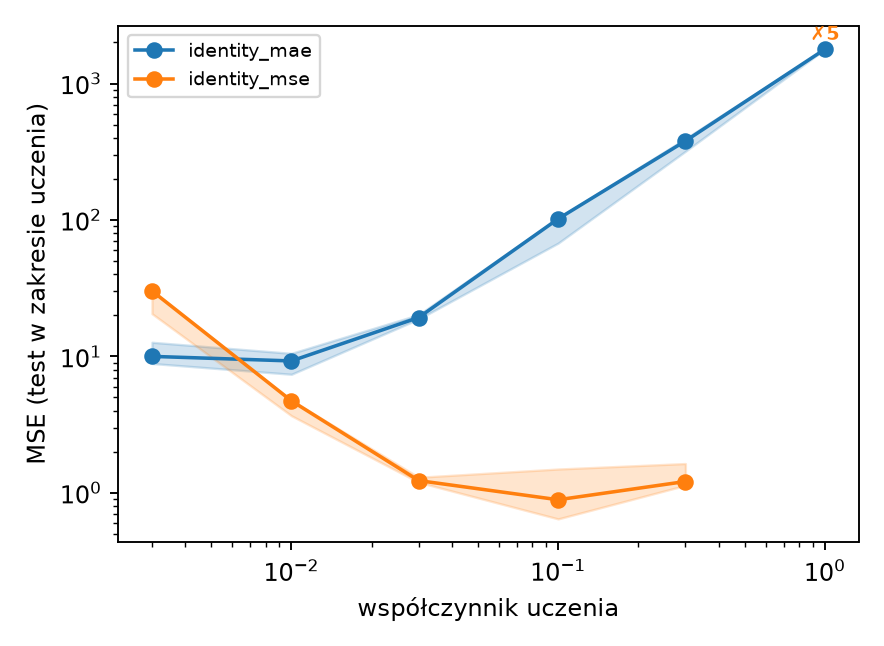
\includegraphics[width=0.7\linewidth]{figures/cube/loss_lr_test_in_mse.png}
  \caption{cube: MSE (test w zakresie uczenia) dla różnych funkcji kosztu w zależności od współczynnika uczenia (mediana i kwartyle; liczba przy krzyżyku nad wykresem to liczba rozbieżnych ziaren).}
  \label{fig:cube:loss_lr_test_in_mse}
\end{figure}

\begin{figure}[htbp]
  \centering
  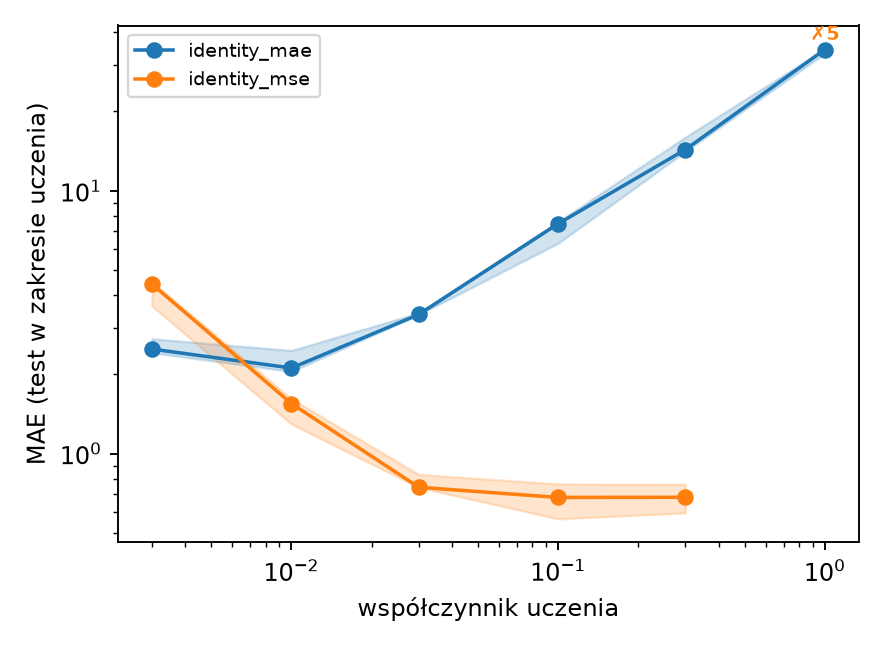
\includegraphics[width=0.7\linewidth]{figures/cube/loss_lr_test_in_mae.png}
  \caption{cube: MAE (test w zakresie uczenia) dla różnych funkcji kosztu w zależności od współczynnika uczenia (mediana i kwartyle; liczba przy krzyżyku nad wykresem to liczba rozbieżnych ziaren).}
  \label{fig:cube:loss_lr_test_in_mae}
\end{figure}

\begin{figure}[htbp]
  \centering
  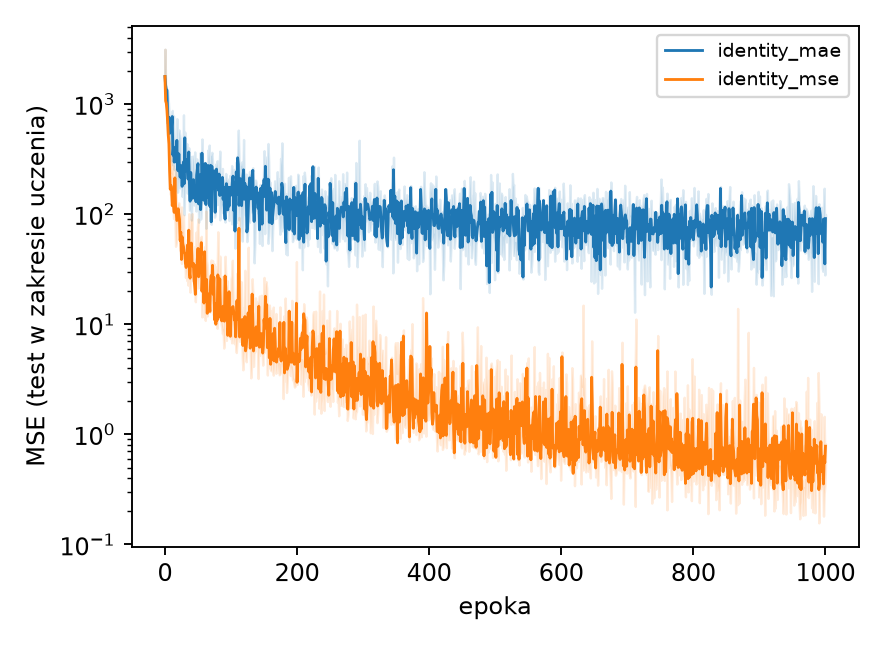
\includegraphics[width=0.7\linewidth]{figures/cube/loss_curve_test_in_mse.png}
  \caption{cube: przebieg MSE (test w zakresie uczenia) w trakcie uczenia dla różnych funkcji kosztu (współczynnik uczenia 0.1).}
  \label{fig:cube:loss_curve_test_in_mse}
\end{figure}

\begin{figure}[htbp]
  \centering
  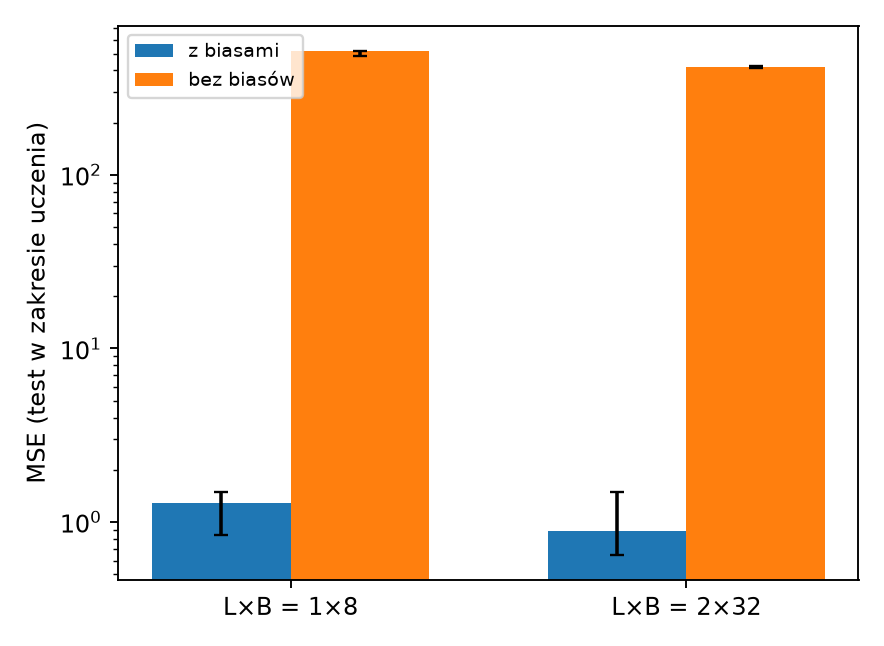
\includegraphics[width=0.7\linewidth]{figures/cube/bias.png}
  \caption{cube: MSE (test w zakresie uczenia) sieci z biasami i bez biasów.}
  \label{fig:cube:bias}
\end{figure}

\begin{figure}[htbp]
  \centering
  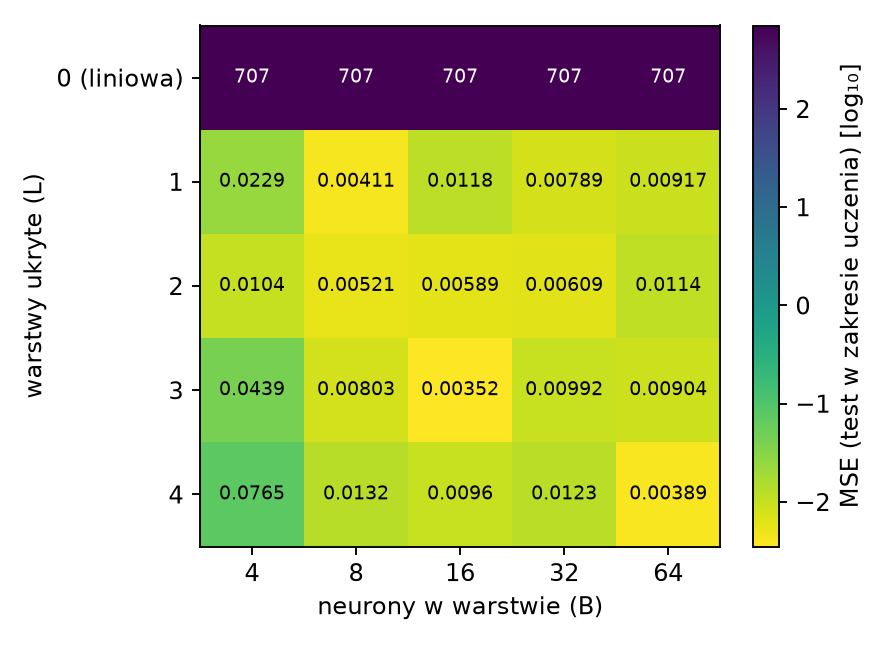
\includegraphics[width=0.7\linewidth]{figures/activation/arch_heatmap_test_in_mse.png}
  \caption{activation: MSE (test w zakresie uczenia) (mediana) w zależności od liczby warstw ukrytych $L$ i neuronów w warstwie $B$.}
  \label{fig:activation:arch_heatmap_test_in_mse}
\end{figure}

\begin{figure}[htbp]
  \centering
  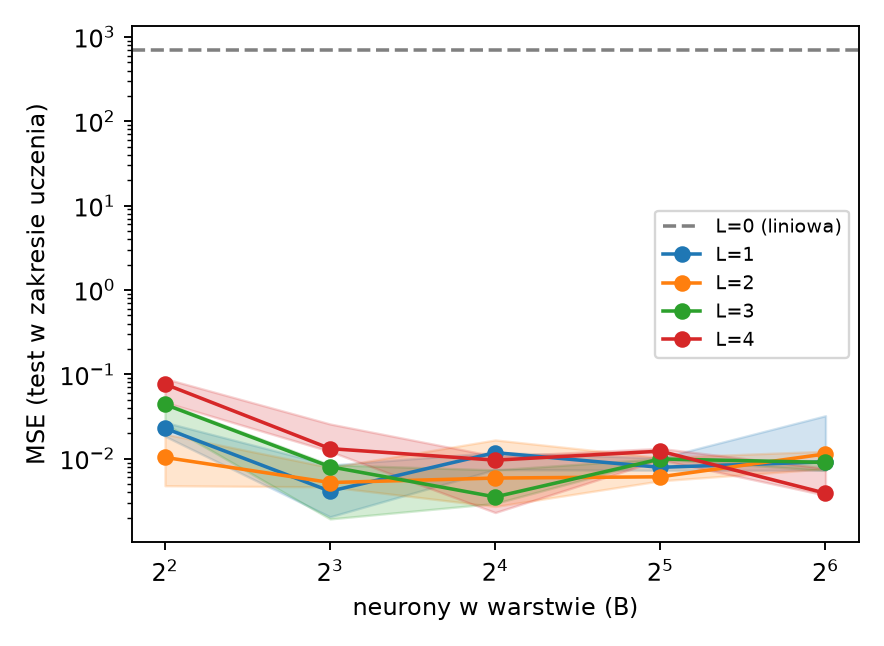
\includegraphics[width=0.7\linewidth]{figures/activation/arch_lines_test_in_mse.png}
  \caption{activation: MSE (test w zakresie uczenia) w zależności od $B$ dla każdej liczby warstw $L$ (mediana i kwartyle po ziarnach).}
  \label{fig:activation:arch_lines_test_in_mse}
\end{figure}

\begin{figure}[htbp]
  \centering
  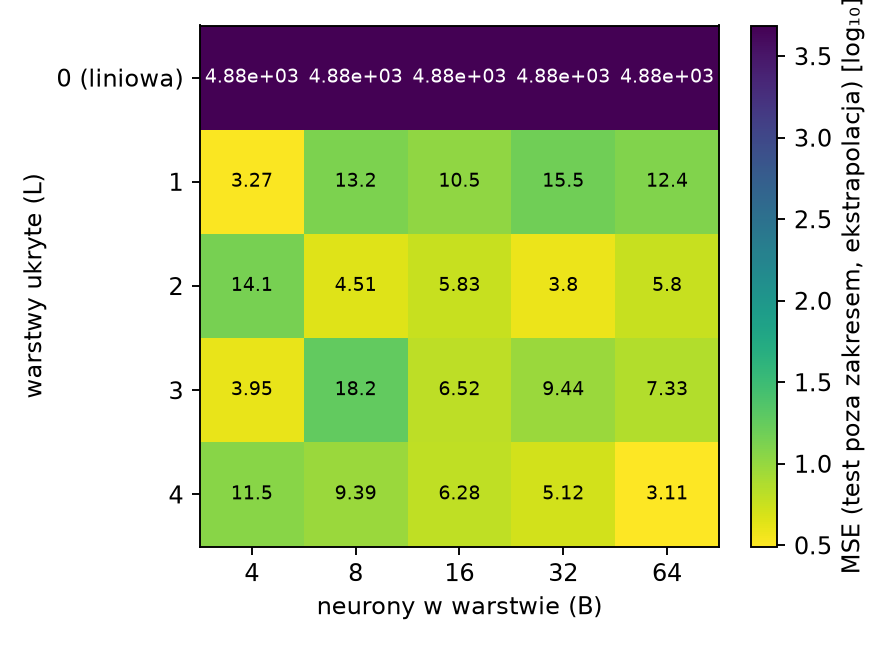
\includegraphics[width=0.7\linewidth]{figures/activation/arch_heatmap_test_out_mse.png}
  \caption{activation: MSE (test poza zakresem, ekstrapolacja) (mediana) w zależności od liczby warstw ukrytych $L$ i neuronów w warstwie $B$.}
  \label{fig:activation:arch_heatmap_test_out_mse}
\end{figure}

\begin{figure}[htbp]
  \centering
  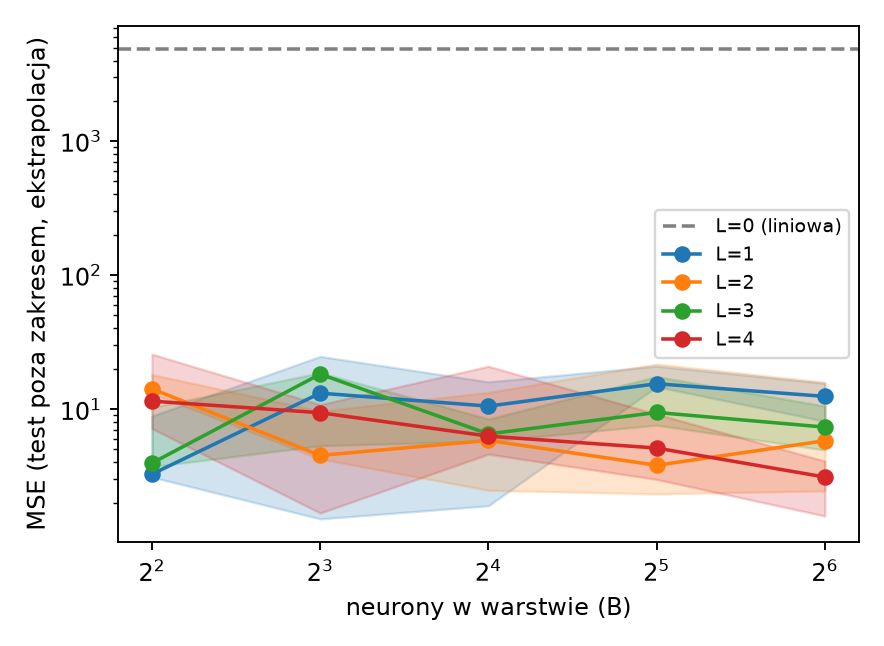
\includegraphics[width=0.7\linewidth]{figures/activation/arch_lines_test_out_mse.png}
  \caption{activation: MSE (test poza zakresem, ekstrapolacja) w zależności od $B$ dla każdej liczby warstw $L$ (mediana i kwartyle po ziarnach).}
  \label{fig:activation:arch_lines_test_out_mse}
\end{figure}

\begin{figure}[htbp]
  \centering
  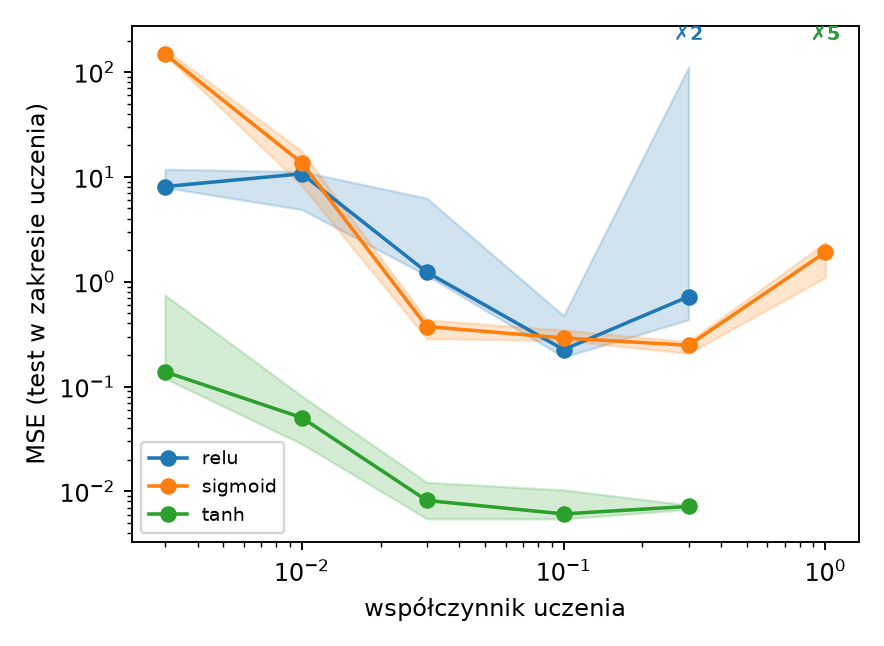
\includegraphics[width=0.7\linewidth]{figures/activation/activation_lr_test_in_mse.png}
  \caption{activation: MSE (test w zakresie uczenia) dla różnych funkcji aktywacji w zależności od współczynnika uczenia (mediana i kwartyle; liczba przy krzyżyku nad wykresem to liczba rozbieżnych ziaren).}
  \label{fig:activation:activation_lr_test_in_mse}
\end{figure}

\begin{figure}[htbp]
  \centering
  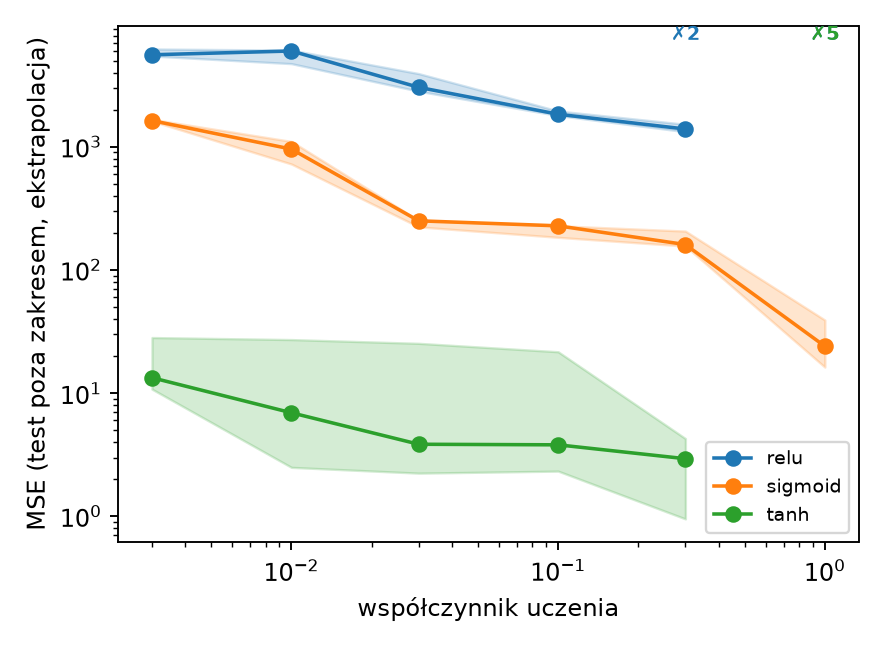
\includegraphics[width=0.7\linewidth]{figures/activation/activation_lr_test_out_mse.png}
  \caption{activation: MSE (test poza zakresem, ekstrapolacja) dla różnych funkcji aktywacji w zależności od współczynnika uczenia (mediana i kwartyle; liczba przy krzyżyku nad wykresem to liczba rozbieżnych ziaren).}
  \label{fig:activation:activation_lr_test_out_mse}
\end{figure}

\begin{figure}[htbp]
  \centering
  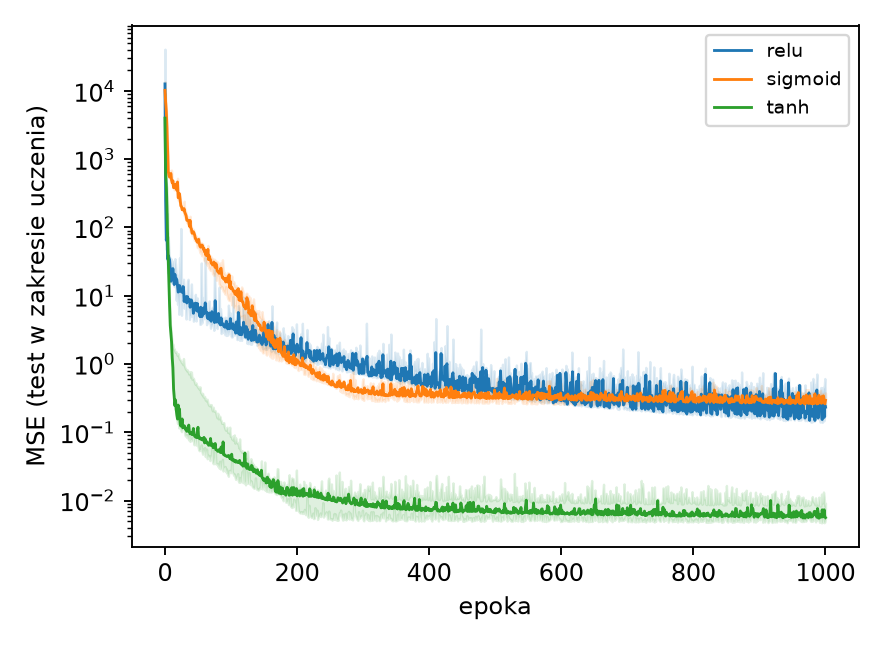
\includegraphics[width=0.7\linewidth]{figures/activation/activation_curve_test_in_mse.png}
  \caption{activation: przebieg MSE (test w zakresie uczenia) w trakcie uczenia dla różnych funkcji aktywacji (współczynnik uczenia 0.1).}
  \label{fig:activation:activation_curve_test_in_mse}
\end{figure}

\begin{figure}[htbp]
  \centering
  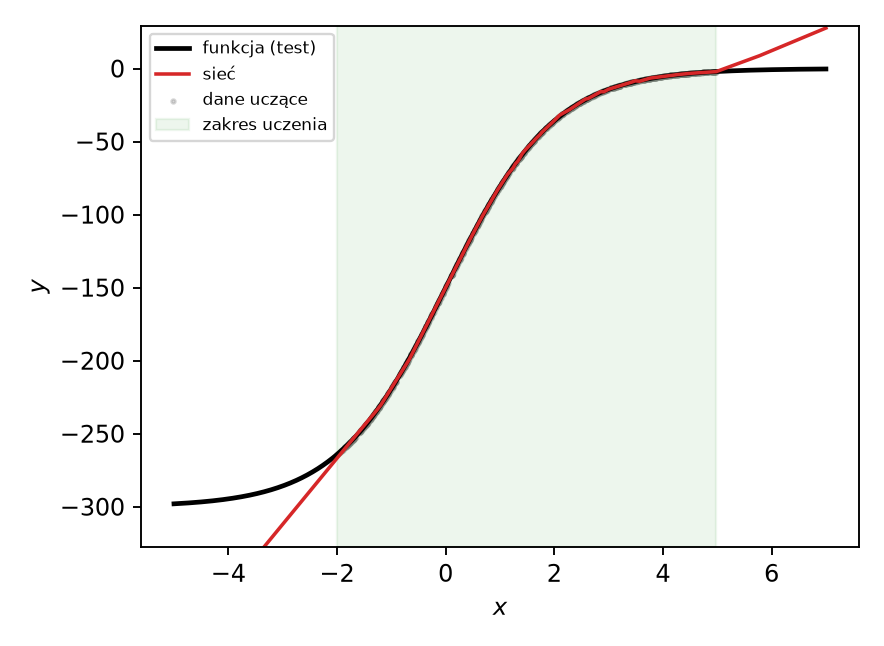
\includegraphics[width=0.7\linewidth]{figures/activation/predictions_relu.png}
  \caption{activation: funkcja nauczona przez sieć z aktywacją relu (ziarno 0) na całym zakresie testu; zielone tło to zakres danych uczących.}
  \label{fig:activation:predictions_relu}
\end{figure}

\begin{figure}[htbp]
  \centering
  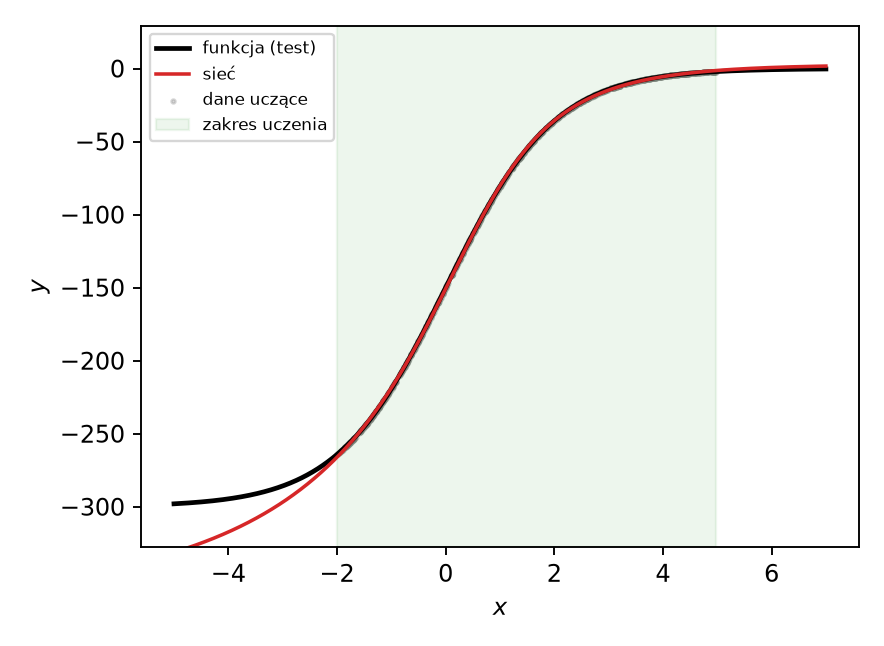
\includegraphics[width=0.7\linewidth]{figures/activation/predictions_sigmoid.png}
  \caption{activation: funkcja nauczona przez sieć z aktywacją sigmoid (ziarno 0) na całym zakresie testu; zielone tło to zakres danych uczących.}
  \label{fig:activation:predictions_sigmoid}
\end{figure}

\begin{figure}[htbp]
  \centering
  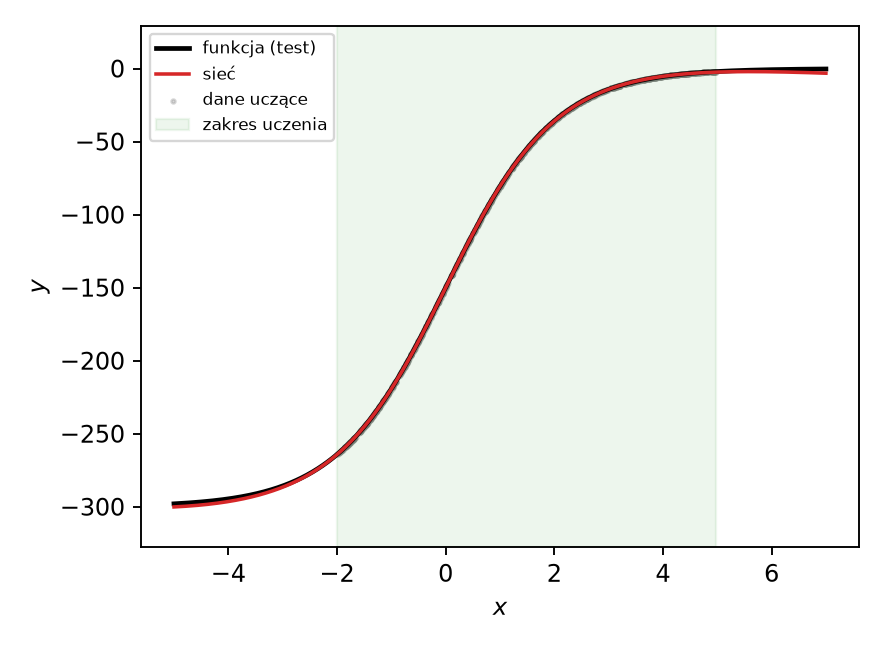
\includegraphics[width=0.7\linewidth]{figures/activation/predictions_tanh.png}
  \caption{activation: funkcja nauczona przez sieć z aktywacją tanh (ziarno 0) na całym zakresie testu; zielone tło to zakres danych uczących.}
  \label{fig:activation:predictions_tanh}
\end{figure}

\begin{figure}[htbp]
  \centering
  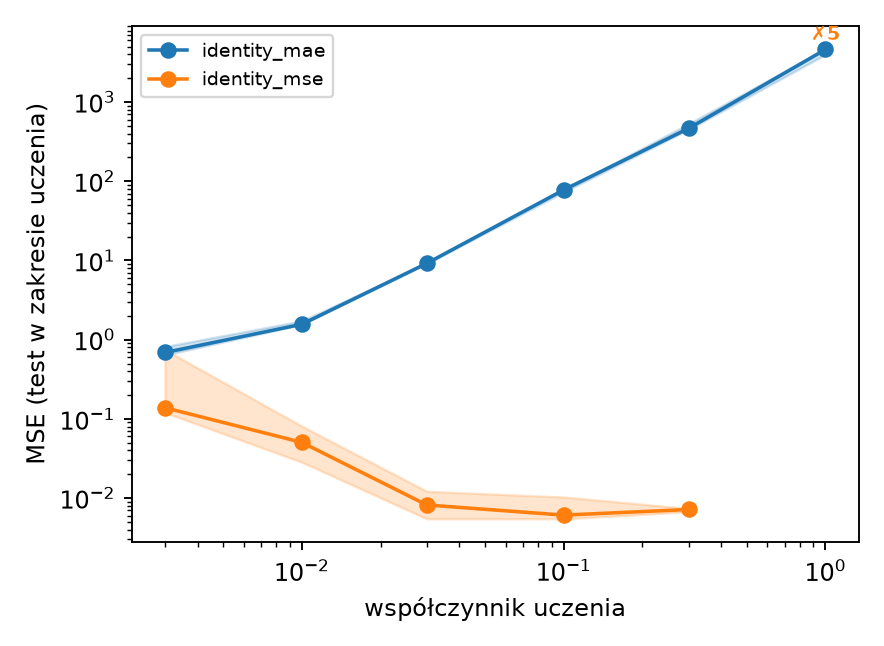
\includegraphics[width=0.7\linewidth]{figures/activation/loss_lr_test_in_mse.png}
  \caption{activation: MSE (test w zakresie uczenia) dla różnych funkcji kosztu w zależności od współczynnika uczenia (mediana i kwartyle; liczba przy krzyżyku nad wykresem to liczba rozbieżnych ziaren).}
  \label{fig:activation:loss_lr_test_in_mse}
\end{figure}

\begin{figure}[htbp]
  \centering
  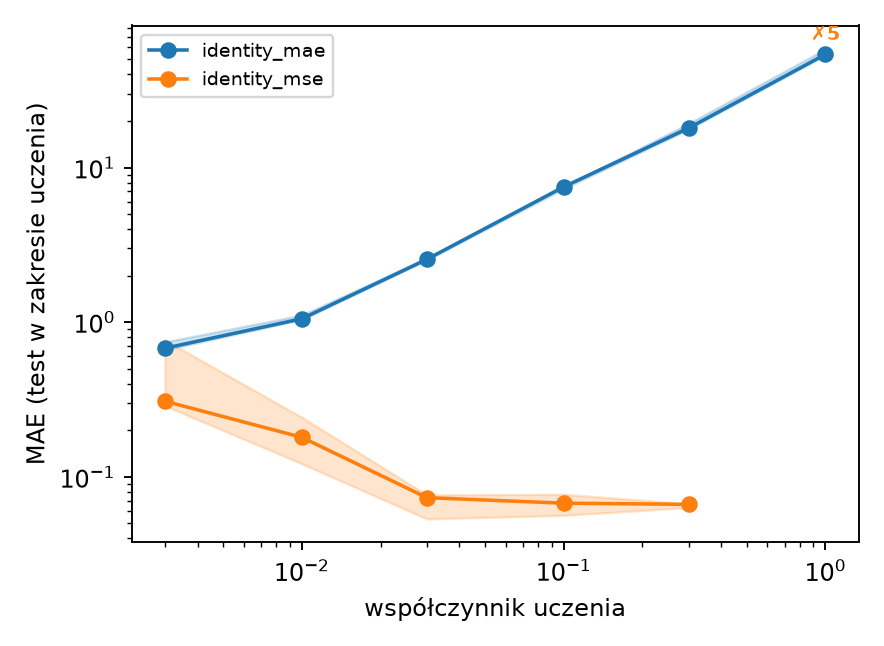
\includegraphics[width=0.7\linewidth]{figures/activation/loss_lr_test_in_mae.png}
  \caption{activation: MAE (test w zakresie uczenia) dla różnych funkcji kosztu w zależności od współczynnika uczenia (mediana i kwartyle; liczba przy krzyżyku nad wykresem to liczba rozbieżnych ziaren).}
  \label{fig:activation:loss_lr_test_in_mae}
\end{figure}

\begin{figure}[htbp]
  \centering
  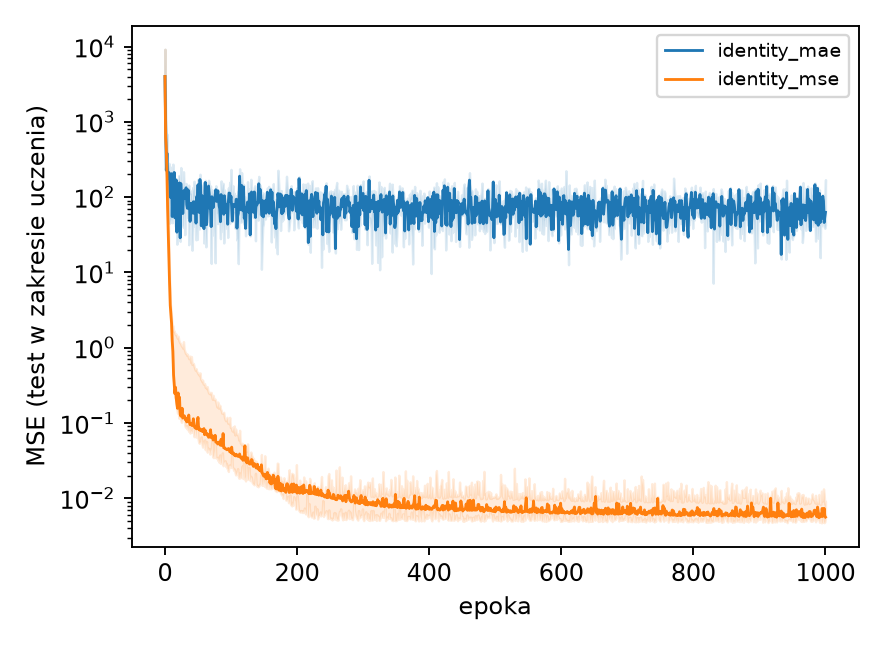
\includegraphics[width=0.7\linewidth]{figures/activation/loss_curve_test_in_mse.png}
  \caption{activation: przebieg MSE (test w zakresie uczenia) w trakcie uczenia dla różnych funkcji kosztu (współczynnik uczenia 0.1).}
  \label{fig:activation:loss_curve_test_in_mse}
\end{figure}

\begin{figure}[htbp]
  \centering
  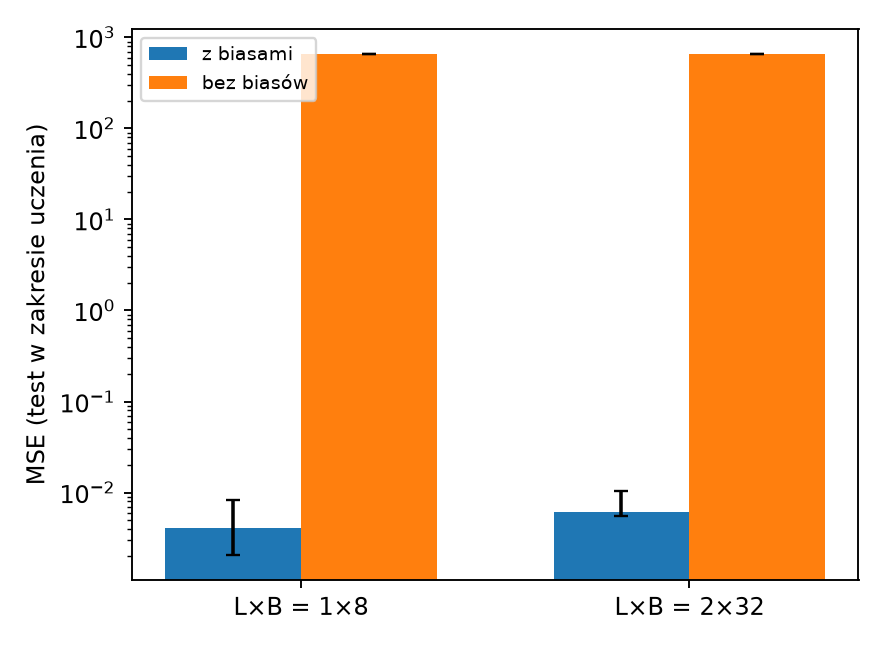
\includegraphics[width=0.7\linewidth]{figures/activation/bias.png}
  \caption{activation: MSE (test w zakresie uczenia) sieci z biasami i bez biasów.}
  \label{fig:activation:bias}
\end{figure}

\begin{figure}[htbp]
  \centering
  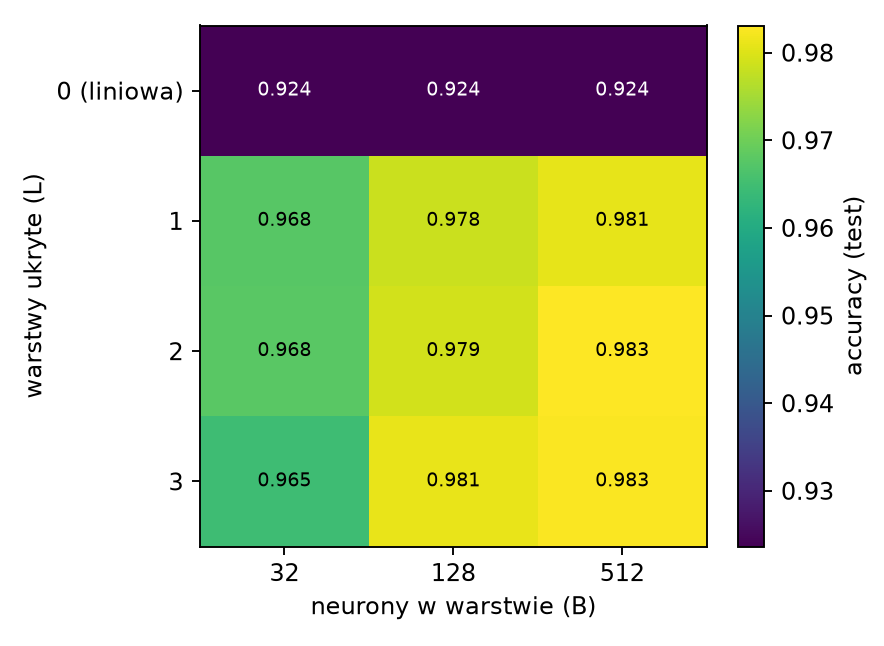
\includegraphics[width=0.7\linewidth]{figures/mnist/arch_heatmap_test_accuracy.png}
  \caption{MNIST: accuracy (test) (mediana) w zależności od liczby warstw ukrytych $L$ i neuronów w warstwie $B$.}
  \label{fig:mnist:arch_heatmap_test_accuracy}
\end{figure}

\begin{figure}[htbp]
  \centering
  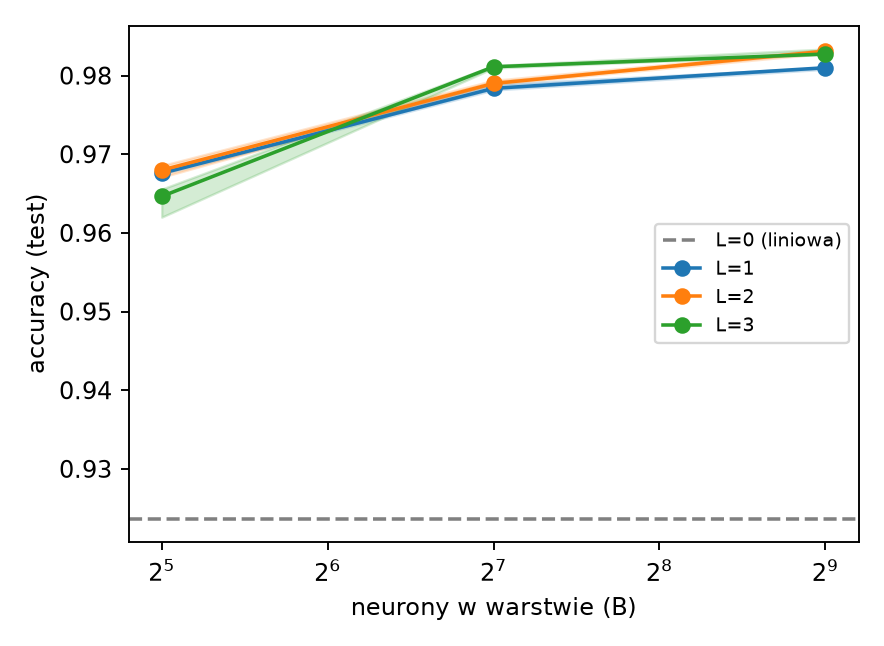
\includegraphics[width=0.7\linewidth]{figures/mnist/arch_lines_test_accuracy.png}
  \caption{MNIST: accuracy (test) w zależności od $B$ dla każdej liczby warstw $L$ (mediana i kwartyle po ziarnach).}
  \label{fig:mnist:arch_lines_test_accuracy}
\end{figure}

\begin{figure}[htbp]
  \centering
  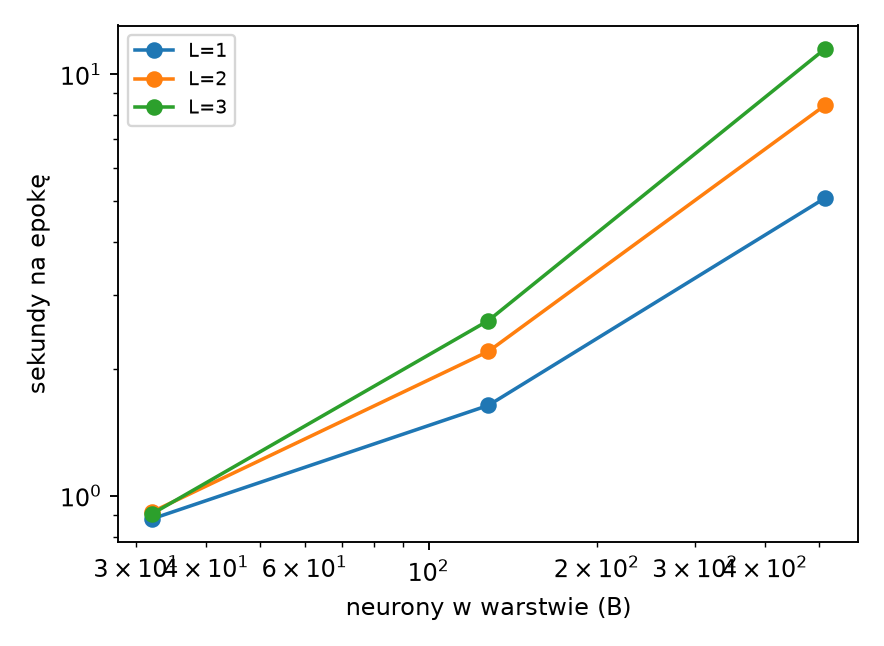
\includegraphics[width=0.7\linewidth]{figures/mnist/time_per_epoch.png}
  \caption{MNIST: czas jednej epoki (uczenie i ewaluacja, jeden wątek) w zależności od architektury.}
  \label{fig:mnist:time_per_epoch}
\end{figure}

\begin{figure}[htbp]
  \centering
  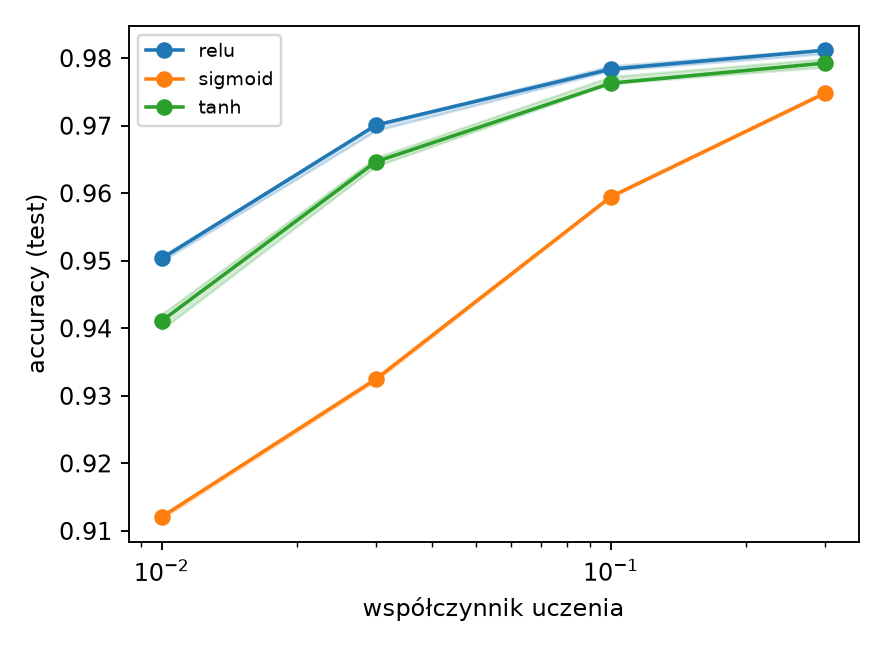
\includegraphics[width=0.7\linewidth]{figures/mnist/activation_lr_test_accuracy.png}
  \caption{MNIST: accuracy (test) dla różnych funkcji aktywacji w zależności od współczynnika uczenia (mediana i kwartyle; liczba przy krzyżyku nad wykresem to liczba rozbieżnych ziaren).}
  \label{fig:mnist:activation_lr_test_accuracy}
\end{figure}

\begin{figure}[htbp]
  \centering
  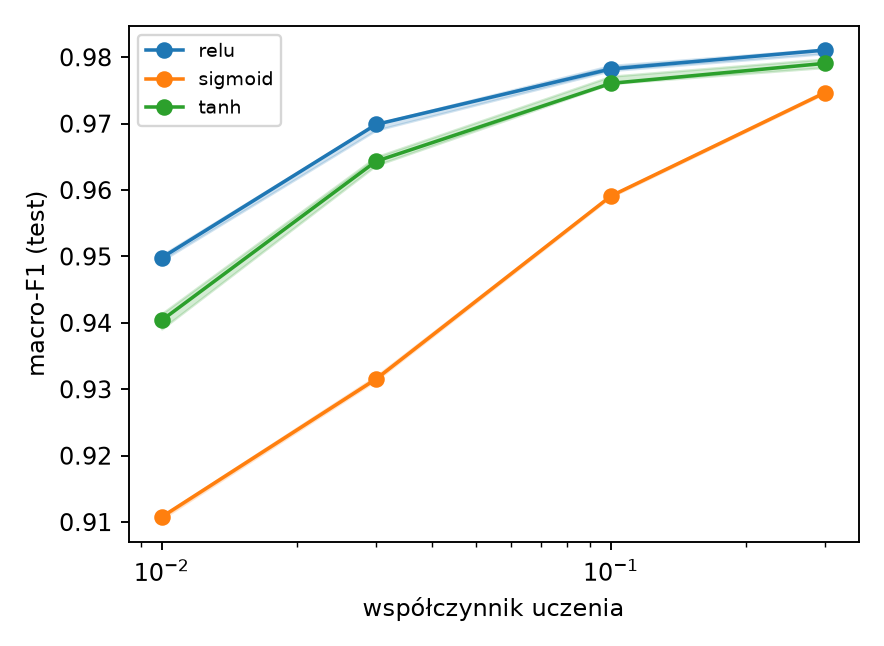
\includegraphics[width=0.7\linewidth]{figures/mnist/activation_lr_test_macro_f1.png}
  \caption{MNIST: macro-F1 (test) dla różnych funkcji aktywacji w zależności od współczynnika uczenia (mediana i kwartyle; liczba przy krzyżyku nad wykresem to liczba rozbieżnych ziaren).}
  \label{fig:mnist:activation_lr_test_macro_f1}
\end{figure}

\begin{figure}[htbp]
  \centering
  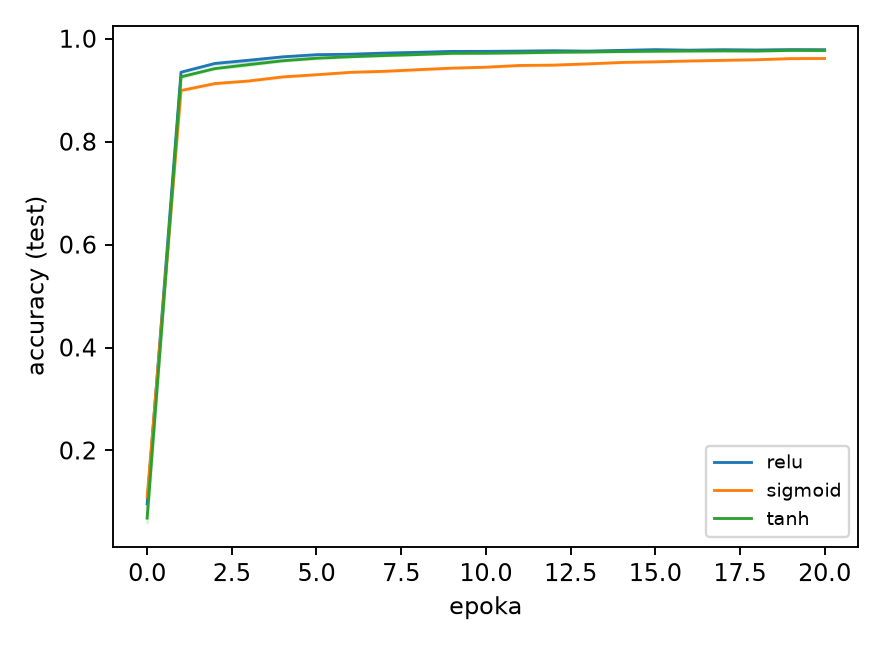
\includegraphics[width=0.7\linewidth]{figures/mnist/activation_curve_test_accuracy.png}
  \caption{MNIST: przebieg accuracy (test) w trakcie uczenia dla różnych funkcji aktywacji (współczynnik uczenia 0.1).}
  \label{fig:mnist:activation_curve_test_accuracy}
\end{figure}

\begin{figure}[htbp]
  \centering
  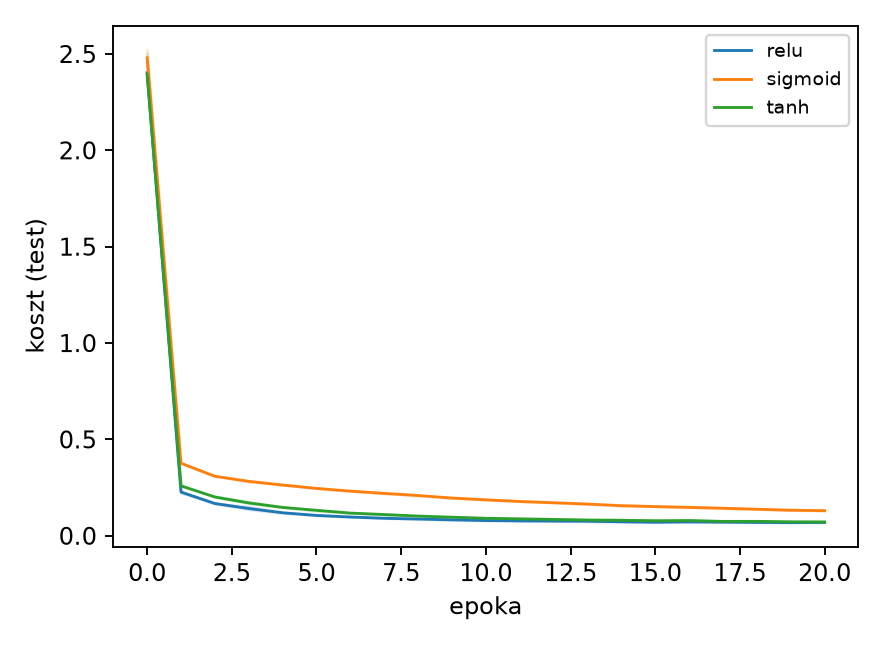
\includegraphics[width=0.7\linewidth]{figures/mnist/activation_curve_test_cost.png}
  \caption{MNIST: przebieg koszt (test) w trakcie uczenia dla różnych funkcji aktywacji (współczynnik uczenia 0.1).}
  \label{fig:mnist:activation_curve_test_cost}
\end{figure}

\begin{figure}[htbp]
  \centering
  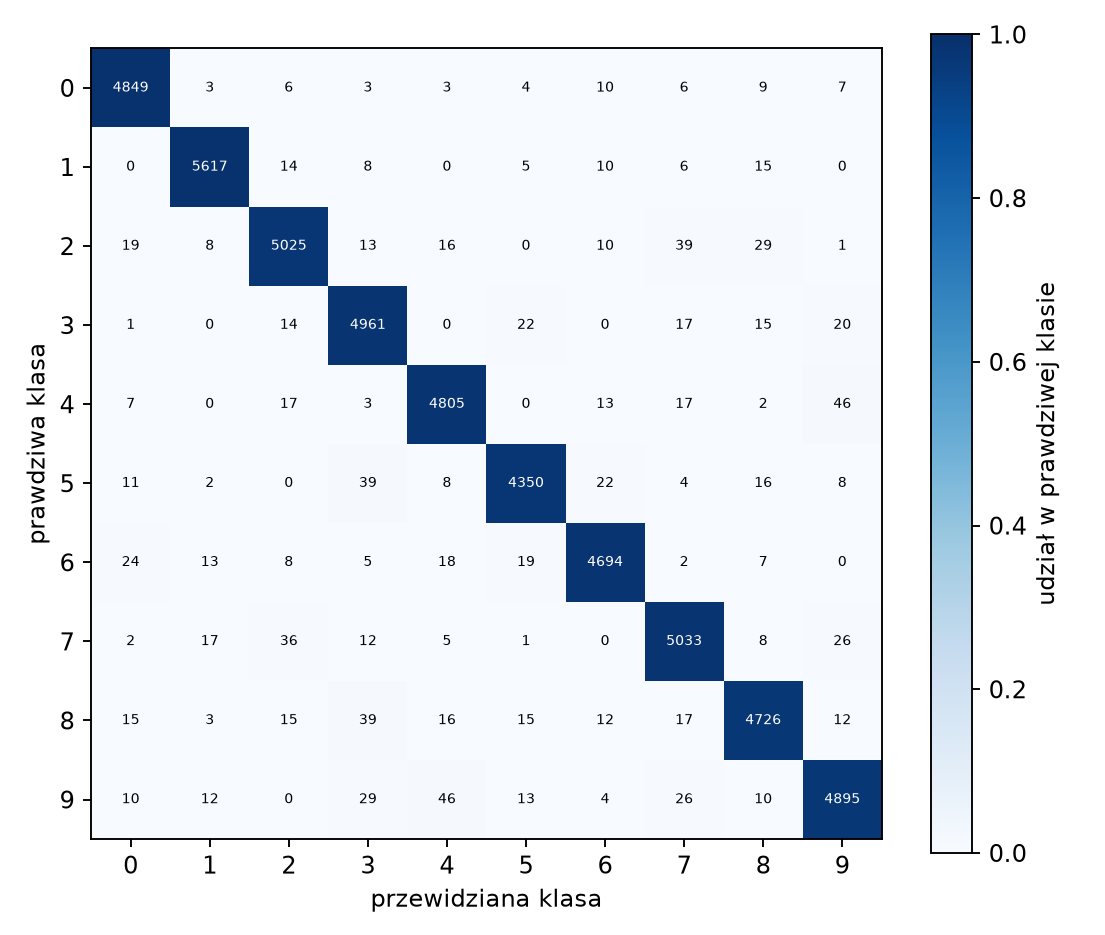
\includegraphics[width=0.7\linewidth]{figures/mnist/confusion_relu_128.png}
  \caption{MNIST: macierz pomyłek na zbiorze testowym, aktywacja relu, architektura 128, suma po 5 ziarnach (accuracy 0.979).}
  \label{fig:mnist:confusion_relu_128}
\end{figure}

\begin{figure}[htbp]
  \centering
  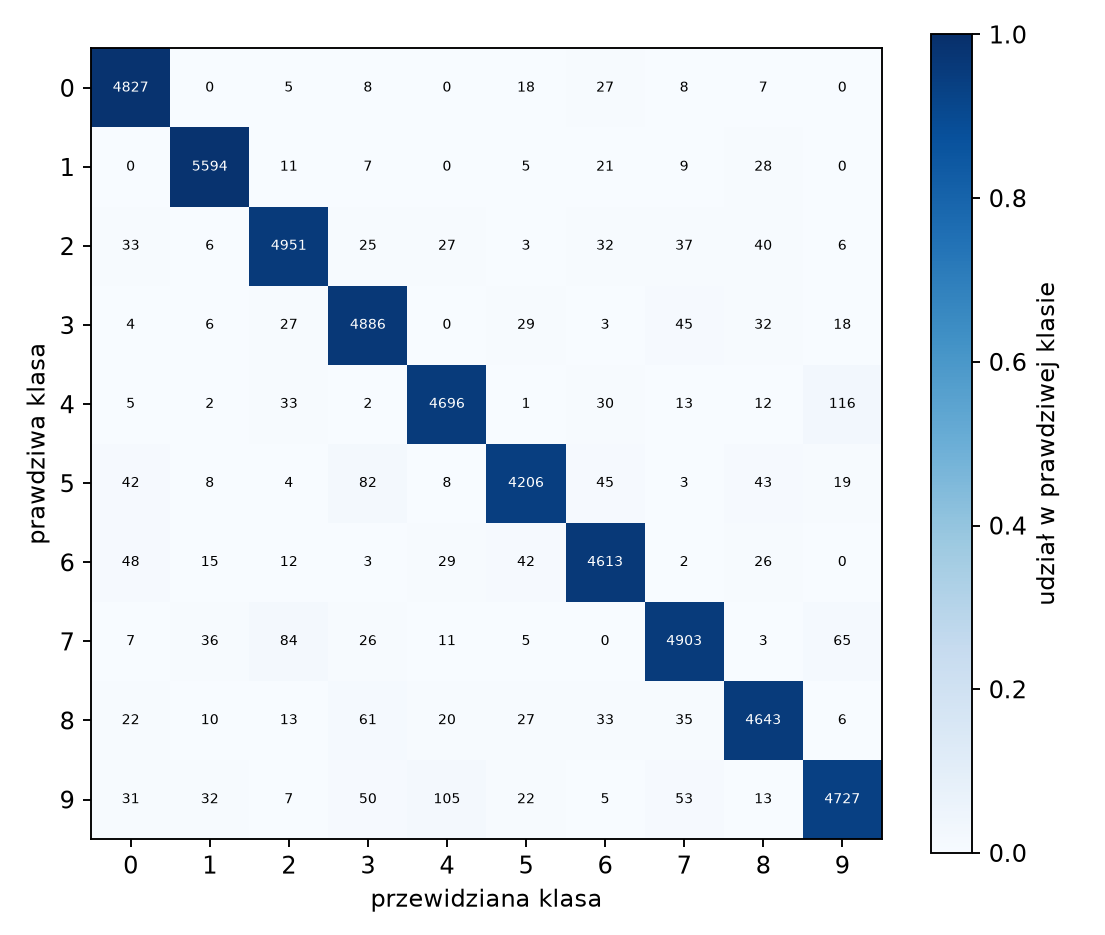
\includegraphics[width=0.7\linewidth]{figures/mnist/confusion_sigmoid_128.png}
  \caption{MNIST: macierz pomyłek na zbiorze testowym, aktywacja sigmoid, architektura 128, suma po 5 ziarnach (accuracy 0.961).}
  \label{fig:mnist:confusion_sigmoid_128}
\end{figure}

\begin{figure}[htbp]
  \centering
  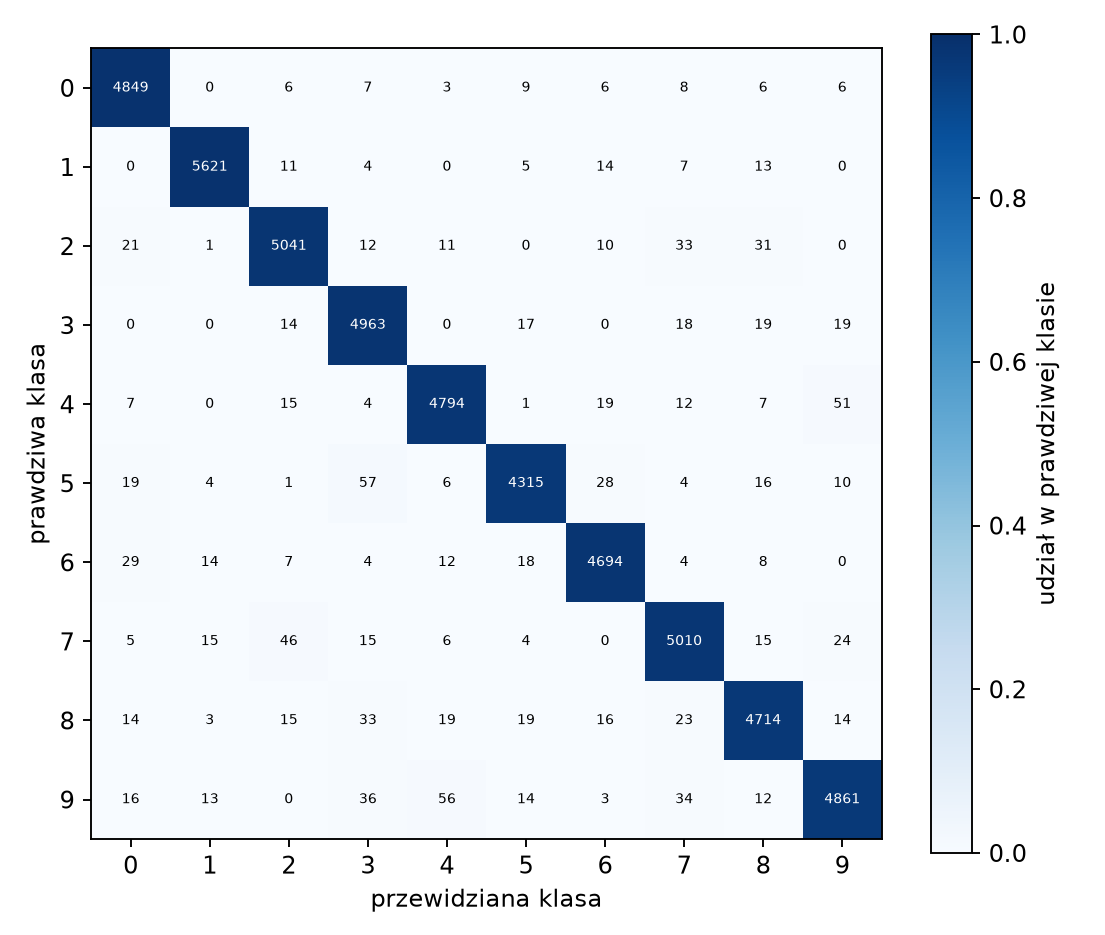
\includegraphics[width=0.7\linewidth]{figures/mnist/confusion_tanh_128.png}
  \caption{MNIST: macierz pomyłek na zbiorze testowym, aktywacja tanh, architektura 128, suma po 5 ziarnach (accuracy 0.977).}
  \label{fig:mnist:confusion_tanh_128}
\end{figure}

\begin{figure}[htbp]
  \centering
  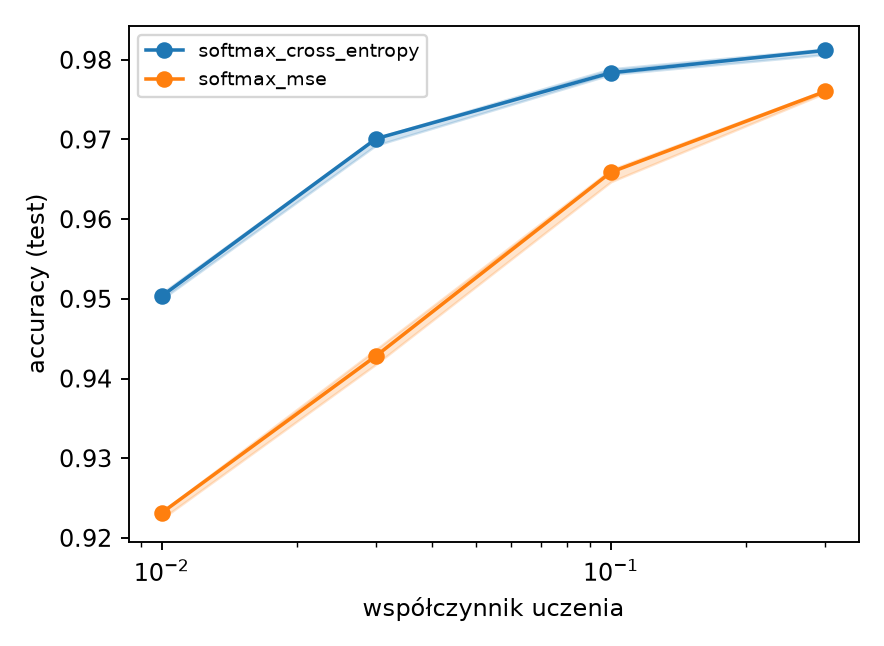
\includegraphics[width=0.7\linewidth]{figures/mnist/loss_lr_test_accuracy.png}
  \caption{MNIST: accuracy (test) dla różnych funkcji kosztu w zależności od współczynnika uczenia (mediana i kwartyle; liczba przy krzyżyku nad wykresem to liczba rozbieżnych ziaren).}
  \label{fig:mnist:loss_lr_test_accuracy}
\end{figure}

\begin{figure}[htbp]
  \centering
  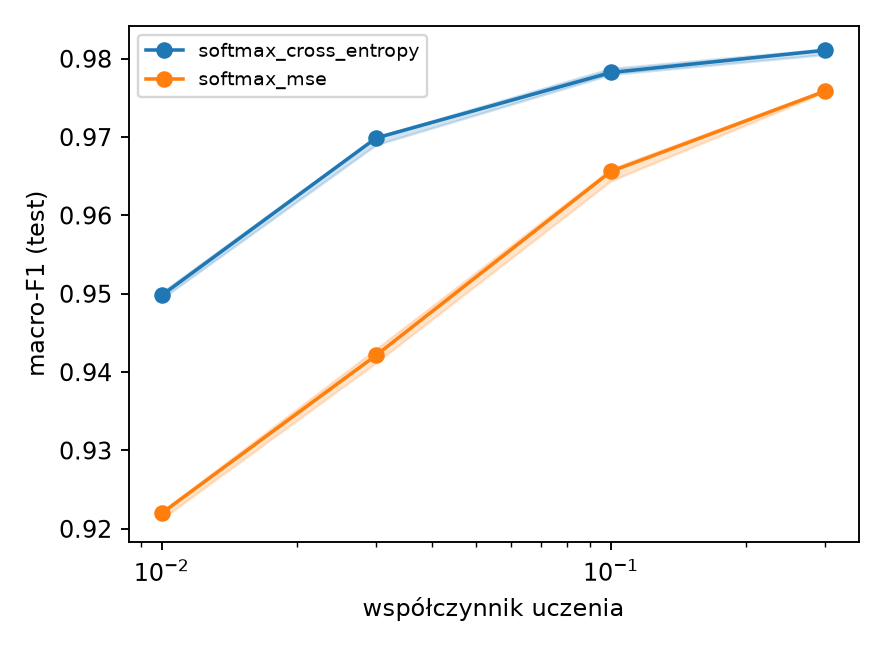
\includegraphics[width=0.7\linewidth]{figures/mnist/loss_lr_test_macro_f1.png}
  \caption{MNIST: macro-F1 (test) dla różnych funkcji kosztu w zależności od współczynnika uczenia (mediana i kwartyle; liczba przy krzyżyku nad wykresem to liczba rozbieżnych ziaren).}
  \label{fig:mnist:loss_lr_test_macro_f1}
\end{figure}

\begin{figure}[htbp]
  \centering
  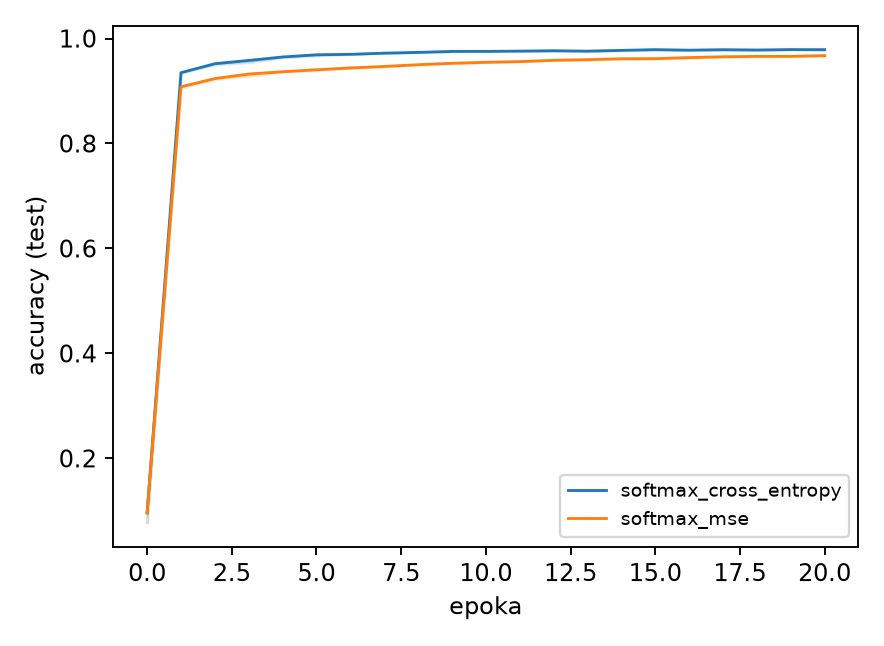
\includegraphics[width=0.7\linewidth]{figures/mnist/loss_curve_test_accuracy.png}
  \caption{MNIST: przebieg accuracy (test) w trakcie uczenia dla różnych funkcji kosztu (współczynnik uczenia 0.1).}
  \label{fig:mnist:loss_curve_test_accuracy}
\end{figure}

\begin{figure}[htbp]
  \centering
  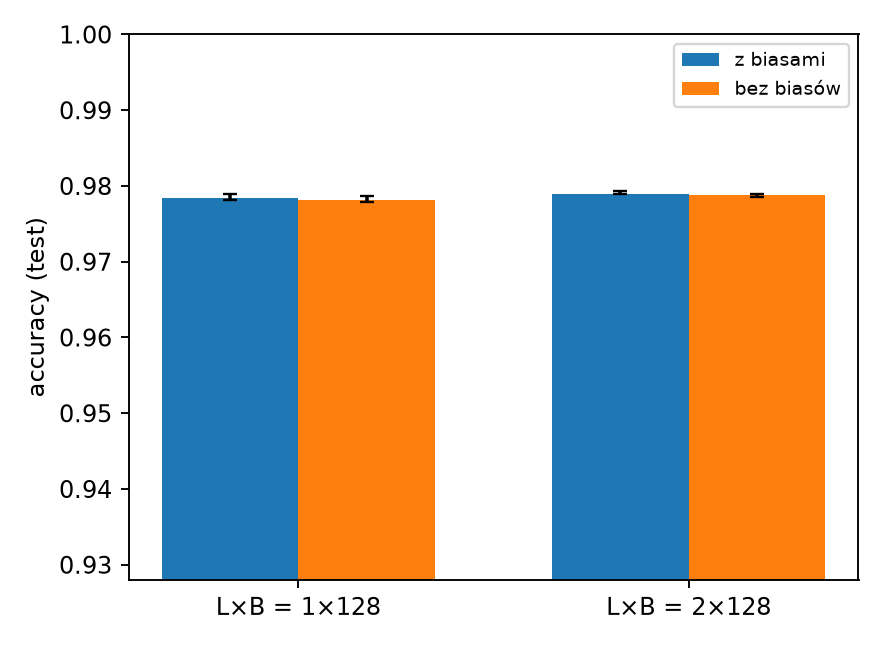
\includegraphics[width=0.7\linewidth]{figures/mnist/bias.png}
  \caption{MNIST: accuracy (test) sieci z biasami i bez biasów.}
  \label{fig:mnist:bias}
\end{figure}
 or copy single blocks.

\begin{figure}[htbp]
  \centering
  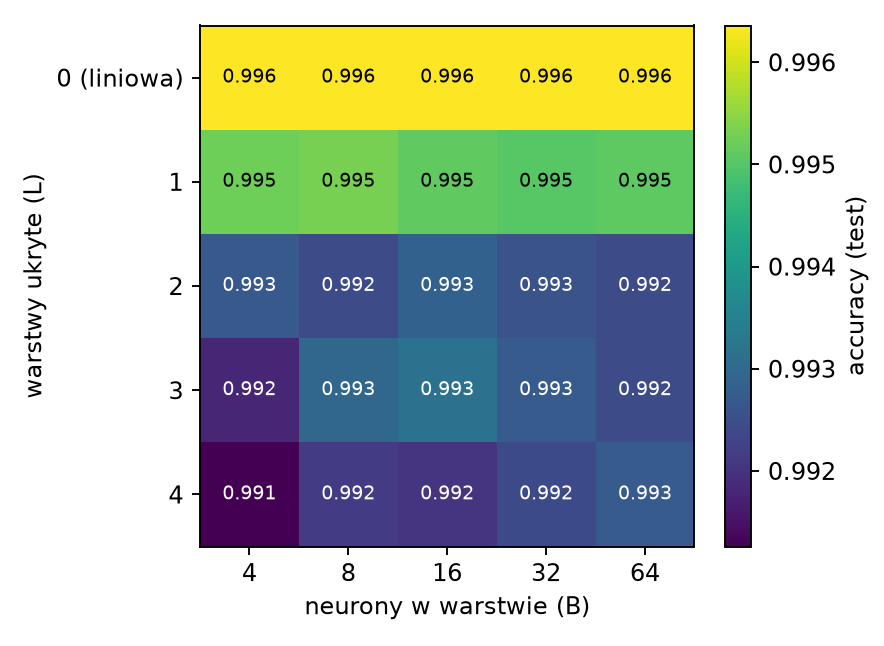
\includegraphics[width=0.7\linewidth]{figures/simple/arch_heatmap_test_accuracy.png}
  \caption{simple: accuracy (test) (mediana) w zależności od liczby warstw ukrytych $L$ i neuronów w warstwie $B$.}
  \label{fig:simple:arch_heatmap_test_accuracy}
\end{figure}

\begin{figure}[htbp]
  \centering
  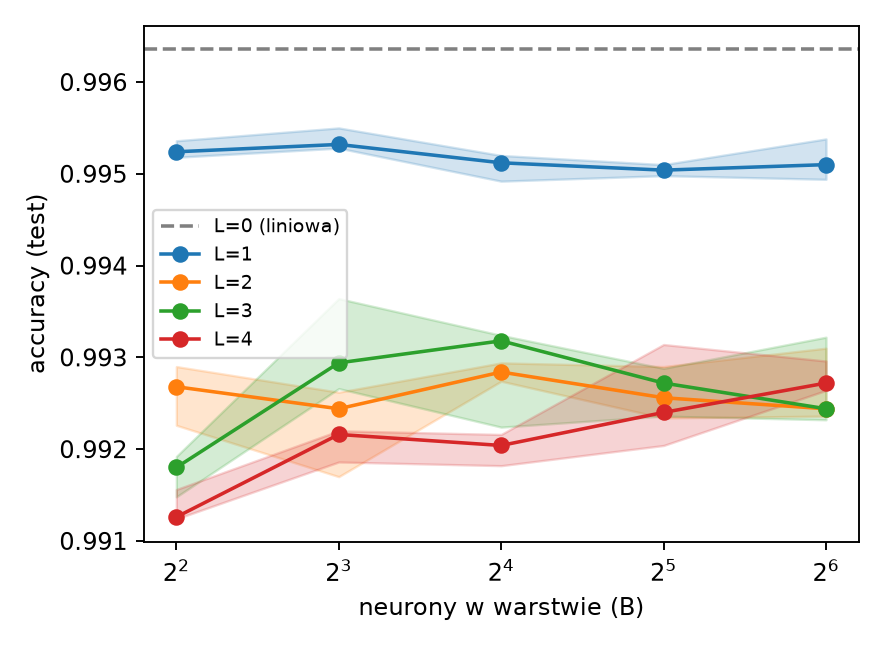
\includegraphics[width=0.7\linewidth]{figures/simple/arch_lines_test_accuracy.png}
  \caption{simple: accuracy (test) w zależności od $B$ dla każdej liczby warstw $L$ (mediana i kwartyle po ziarnach).}
  \label{fig:simple:arch_lines_test_accuracy}
\end{figure}

\begin{figure}[htbp]
  \centering
  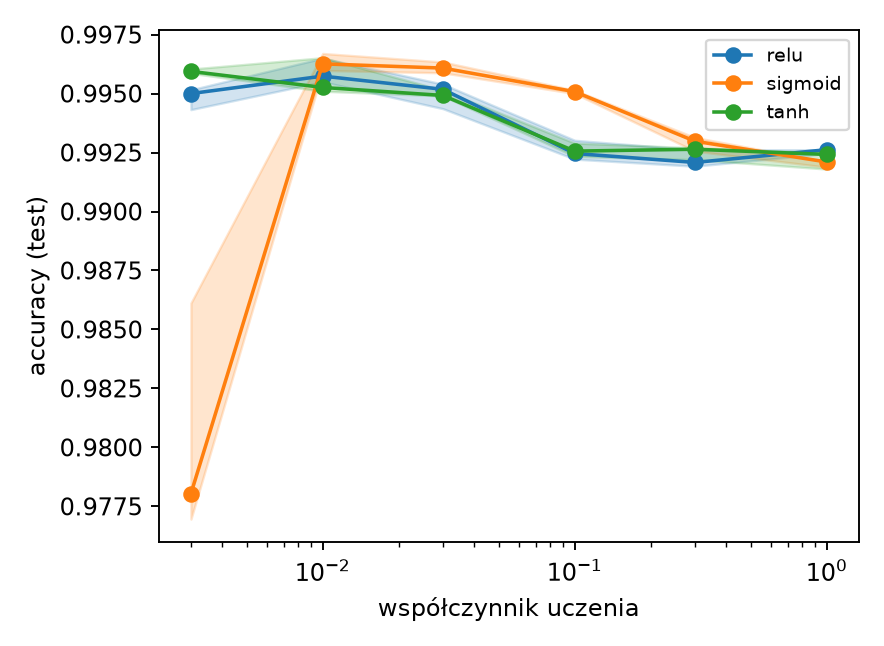
\includegraphics[width=0.7\linewidth]{figures/simple/activation_lr_test_accuracy.png}
  \caption{simple: accuracy (test) dla różnych funkcji aktywacji w zależności od współczynnika uczenia (mediana i kwartyle; liczba przy krzyżyku nad wykresem to liczba rozbieżnych ziaren).}
  \label{fig:simple:activation_lr_test_accuracy}
\end{figure}

\begin{figure}[htbp]
  \centering
  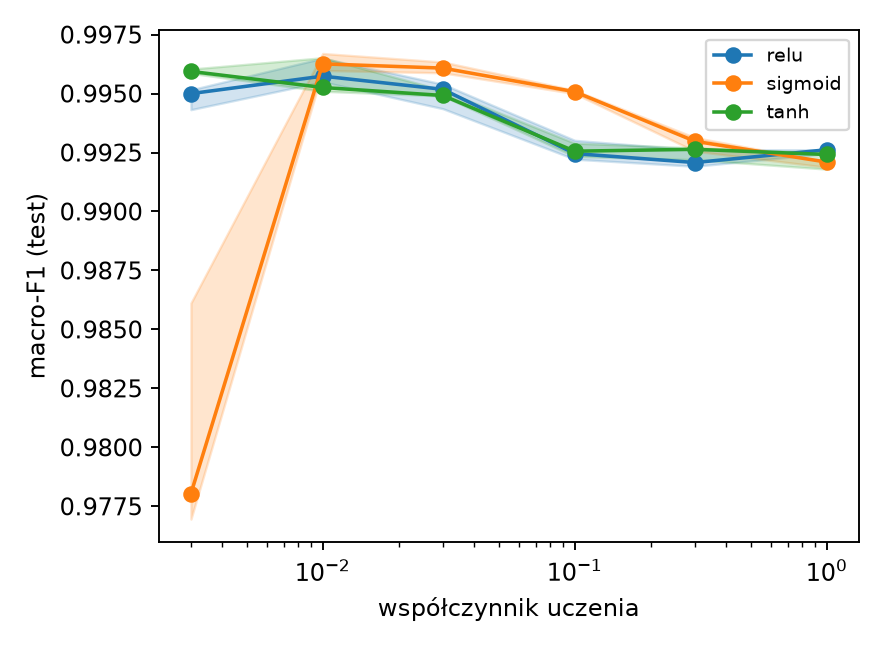
\includegraphics[width=0.7\linewidth]{figures/simple/activation_lr_test_macro_f1.png}
  \caption{simple: macro-F1 (test) dla różnych funkcji aktywacji w zależności od współczynnika uczenia (mediana i kwartyle; liczba przy krzyżyku nad wykresem to liczba rozbieżnych ziaren).}
  \label{fig:simple:activation_lr_test_macro_f1}
\end{figure}

\begin{figure}[htbp]
  \centering
  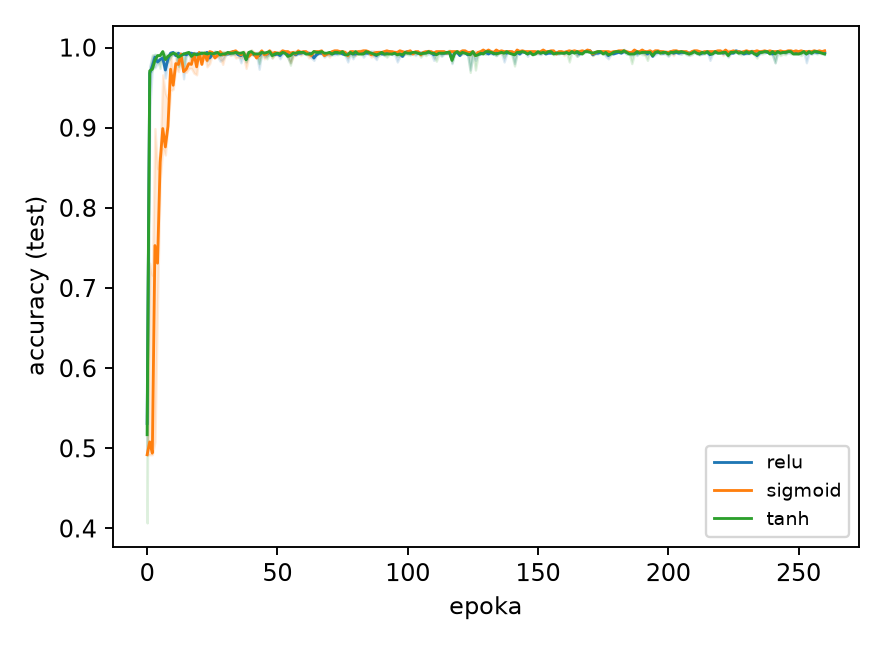
\includegraphics[width=0.7\linewidth]{figures/simple/activation_curve_test_accuracy.png}
  \caption{simple: przebieg accuracy (test) w trakcie uczenia dla różnych funkcji aktywacji (współczynnik uczenia 0.1).}
  \label{fig:simple:activation_curve_test_accuracy}
\end{figure}

\begin{figure}[htbp]
  \centering
  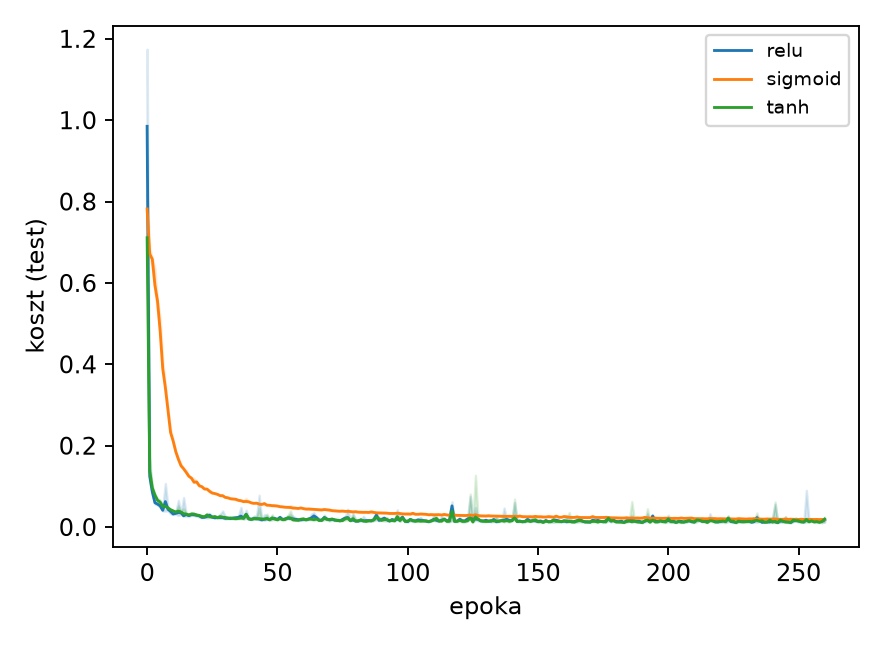
\includegraphics[width=0.7\linewidth]{figures/simple/activation_curve_test_cost.png}
  \caption{simple: przebieg koszt (test) w trakcie uczenia dla różnych funkcji aktywacji (współczynnik uczenia 0.1).}
  \label{fig:simple:activation_curve_test_cost}
\end{figure}

\begin{figure}[htbp]
  \centering
  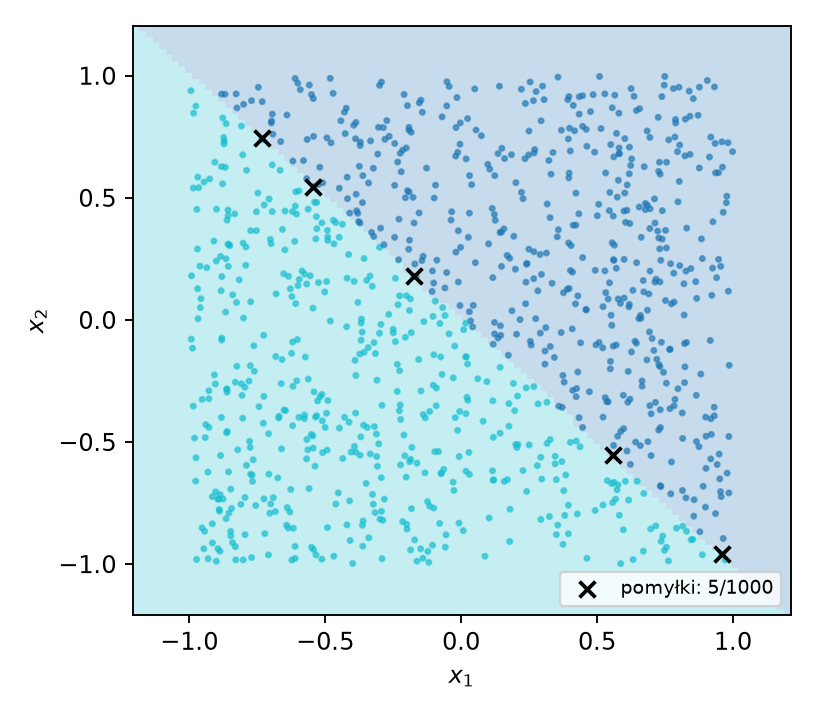
\includegraphics[width=0.7\linewidth]{figures/simple/predictions_relu.png}
  \caption{simple: obszary decyzyjne sieci z aktywacją relu (ziarno 0). Punkty testowe w kolorze prawdziwej klasy, × oznacza pomyłkę (accuracy 0.995).}
  \label{fig:simple:predictions_relu}
\end{figure}

\begin{figure}[htbp]
  \centering
  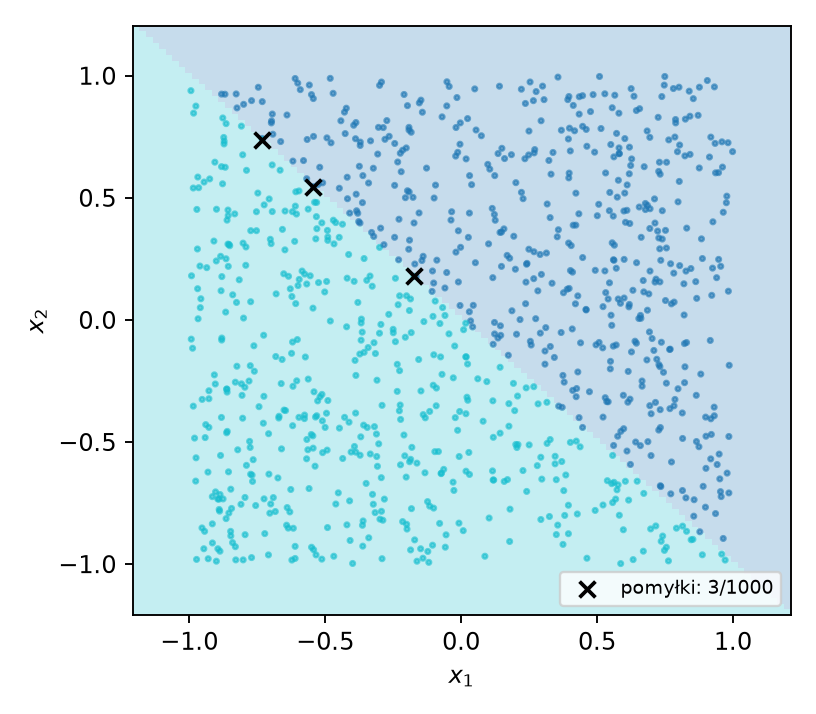
\includegraphics[width=0.7\linewidth]{figures/simple/predictions_sigmoid.png}
  \caption{simple: obszary decyzyjne sieci z aktywacją sigmoid (ziarno 0). Punkty testowe w kolorze prawdziwej klasy, × oznacza pomyłkę (accuracy 0.997).}
  \label{fig:simple:predictions_sigmoid}
\end{figure}

\begin{figure}[htbp]
  \centering
  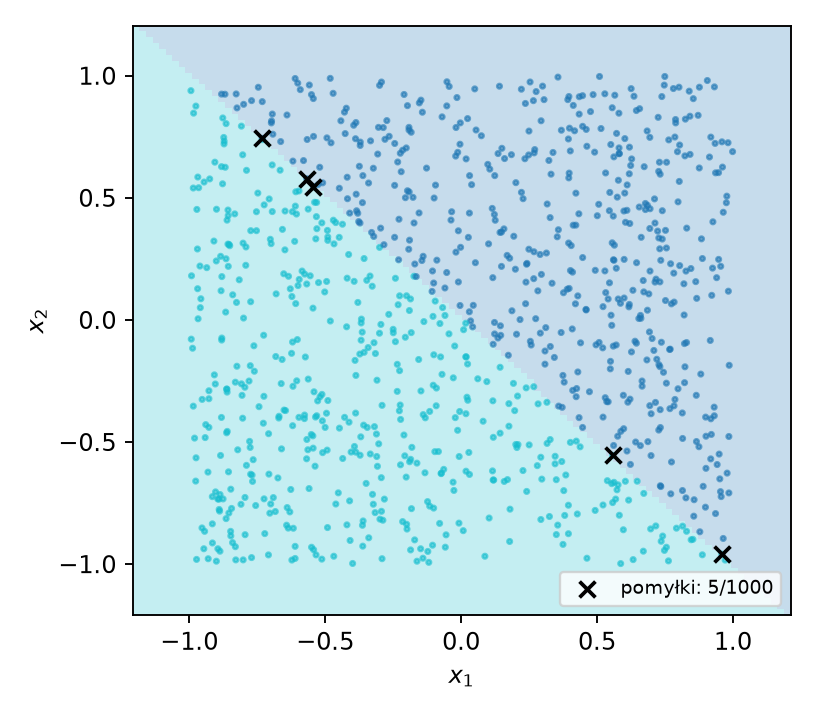
\includegraphics[width=0.7\linewidth]{figures/simple/predictions_tanh.png}
  \caption{simple: obszary decyzyjne sieci z aktywacją tanh (ziarno 0). Punkty testowe w kolorze prawdziwej klasy, × oznacza pomyłkę (accuracy 0.995).}
  \label{fig:simple:predictions_tanh}
\end{figure}

\begin{figure}[htbp]
  \centering
  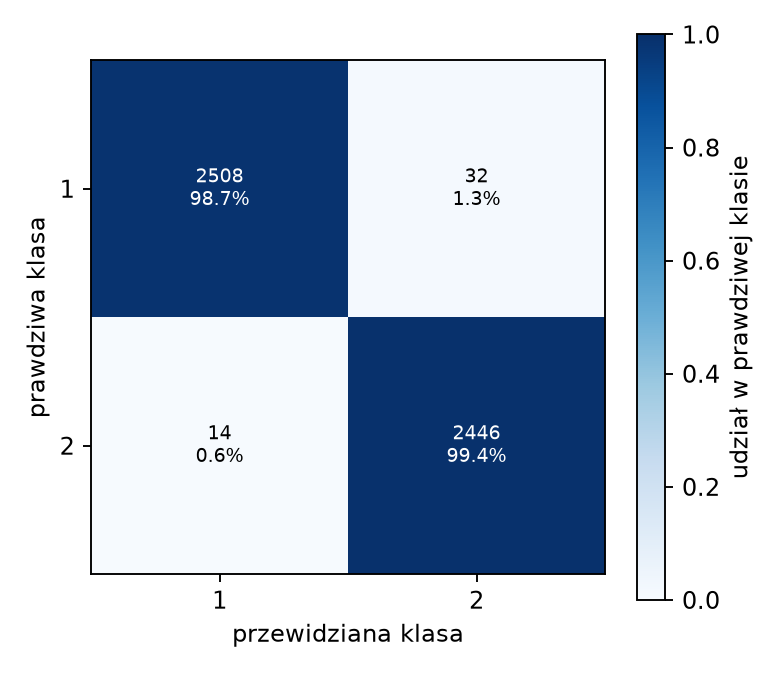
\includegraphics[width=0.7\linewidth]{figures/simple/confusion_relu_32x32.png}
  \caption{simple: macierz pomyłek na zbiorze testowym, aktywacja relu, architektura 32x32, suma po 5 ziarnach (accuracy 0.991).}
  \label{fig:simple:confusion_relu_32x32}
\end{figure}

\begin{figure}[htbp]
  \centering
  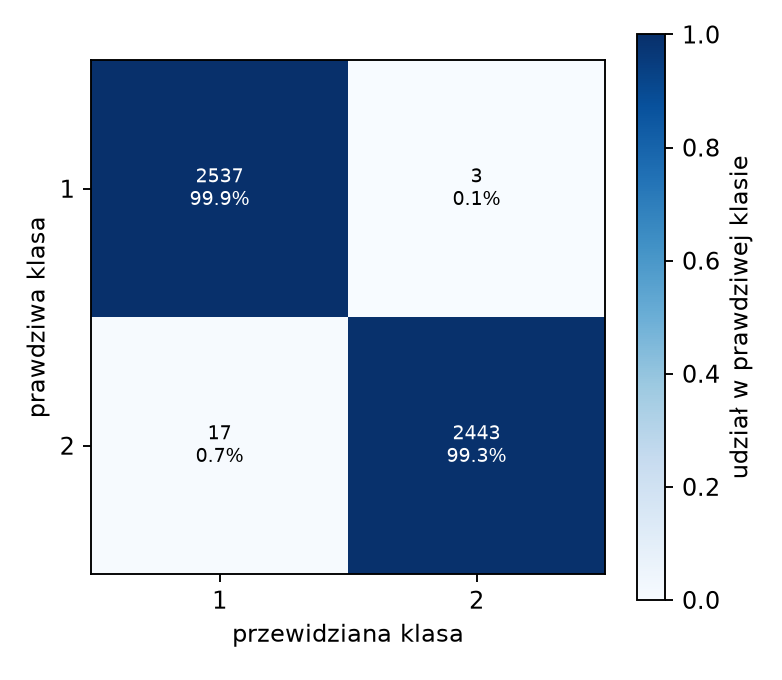
\includegraphics[width=0.7\linewidth]{figures/simple/confusion_sigmoid_32x32.png}
  \caption{simple: macierz pomyłek na zbiorze testowym, aktywacja sigmoid, architektura 32x32, suma po 5 ziarnach (accuracy 0.996).}
  \label{fig:simple:confusion_sigmoid_32x32}
\end{figure}

\begin{figure}[htbp]
  \centering
  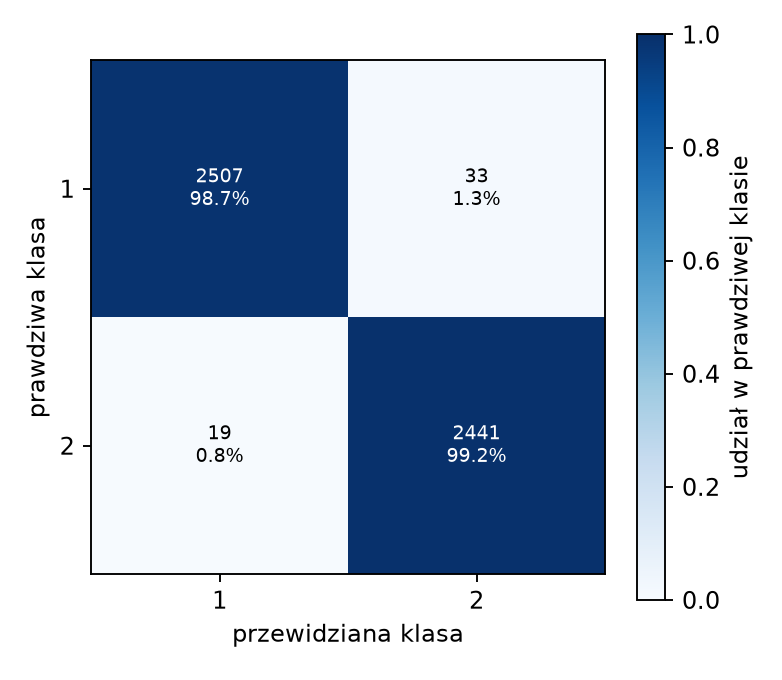
\includegraphics[width=0.7\linewidth]{figures/simple/confusion_tanh_32x32.png}
  \caption{simple: macierz pomyłek na zbiorze testowym, aktywacja tanh, architektura 32x32, suma po 5 ziarnach (accuracy 0.990).}
  \label{fig:simple:confusion_tanh_32x32}
\end{figure}

\begin{figure}[htbp]
  \centering
  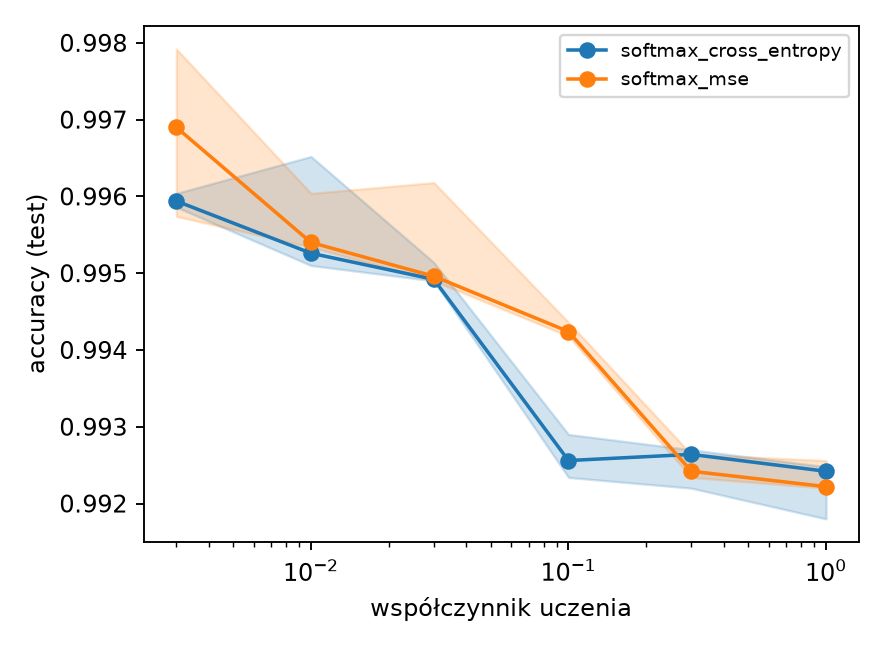
\includegraphics[width=0.7\linewidth]{figures/simple/loss_lr_test_accuracy.png}
  \caption{simple: accuracy (test) dla różnych funkcji kosztu w zależności od współczynnika uczenia (mediana i kwartyle; liczba przy krzyżyku nad wykresem to liczba rozbieżnych ziaren).}
  \label{fig:simple:loss_lr_test_accuracy}
\end{figure}

\begin{figure}[htbp]
  \centering
  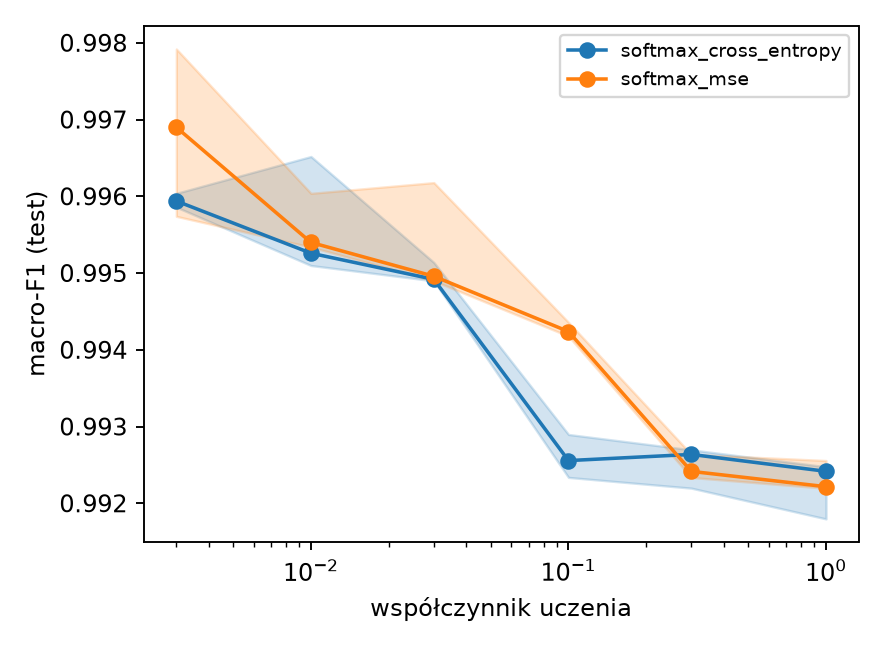
\includegraphics[width=0.7\linewidth]{figures/simple/loss_lr_test_macro_f1.png}
  \caption{simple: macro-F1 (test) dla różnych funkcji kosztu w zależności od współczynnika uczenia (mediana i kwartyle; liczba przy krzyżyku nad wykresem to liczba rozbieżnych ziaren).}
  \label{fig:simple:loss_lr_test_macro_f1}
\end{figure}

\begin{figure}[htbp]
  \centering
  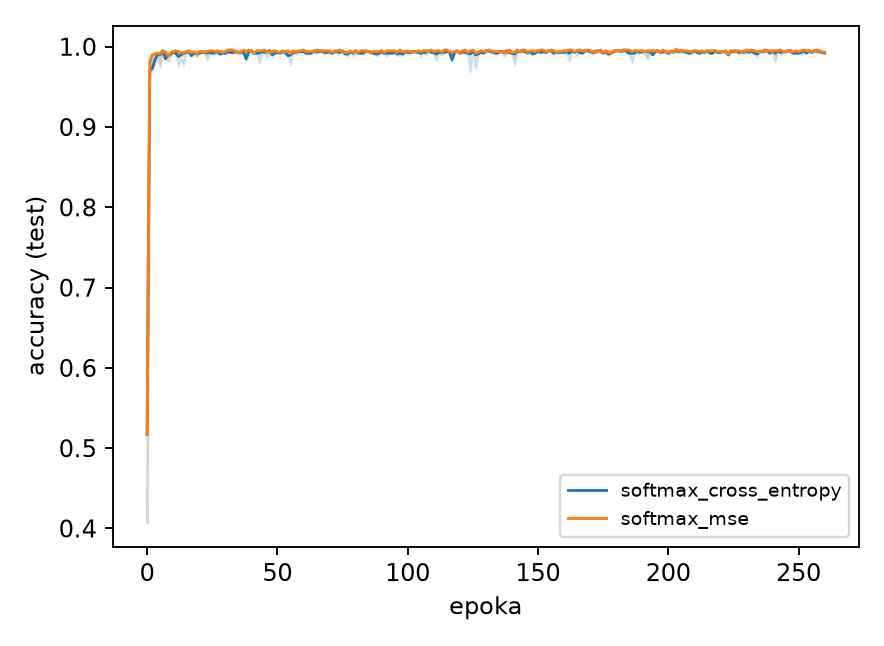
\includegraphics[width=0.7\linewidth]{figures/simple/loss_curve_test_accuracy.png}
  \caption{simple: przebieg accuracy (test) w trakcie uczenia dla różnych funkcji kosztu (współczynnik uczenia 0.1).}
  \label{fig:simple:loss_curve_test_accuracy}
\end{figure}

\begin{figure}[htbp]
  \centering
  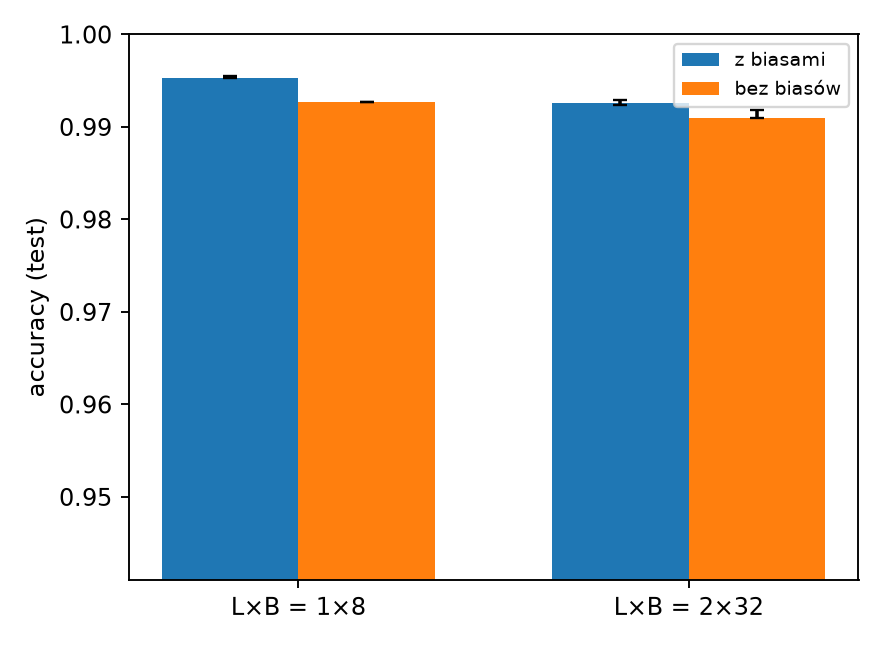
\includegraphics[width=0.7\linewidth]{figures/simple/bias.png}
  \caption{simple: accuracy (test) sieci z biasami i bez biasów.}
  \label{fig:simple:bias}
\end{figure}

\begin{figure}[htbp]
  \centering
  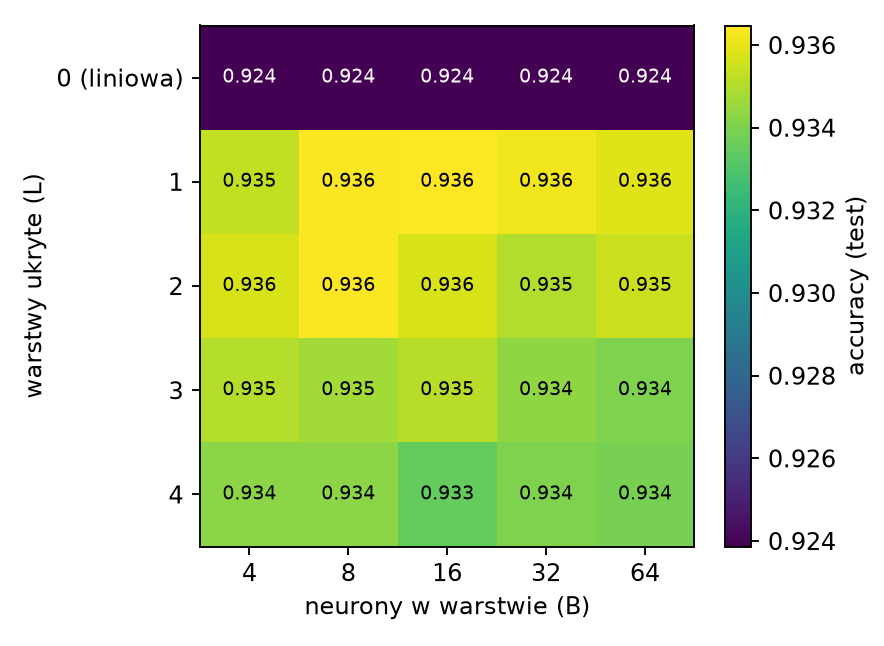
\includegraphics[width=0.7\linewidth]{figures/three_gauss/arch_heatmap_test_accuracy.png}
  \caption{three\_gauss: accuracy (test) (mediana) w zależności od liczby warstw ukrytych $L$ i neuronów w warstwie $B$.}
  \label{fig:three_gauss:arch_heatmap_test_accuracy}
\end{figure}

\begin{figure}[htbp]
  \centering
  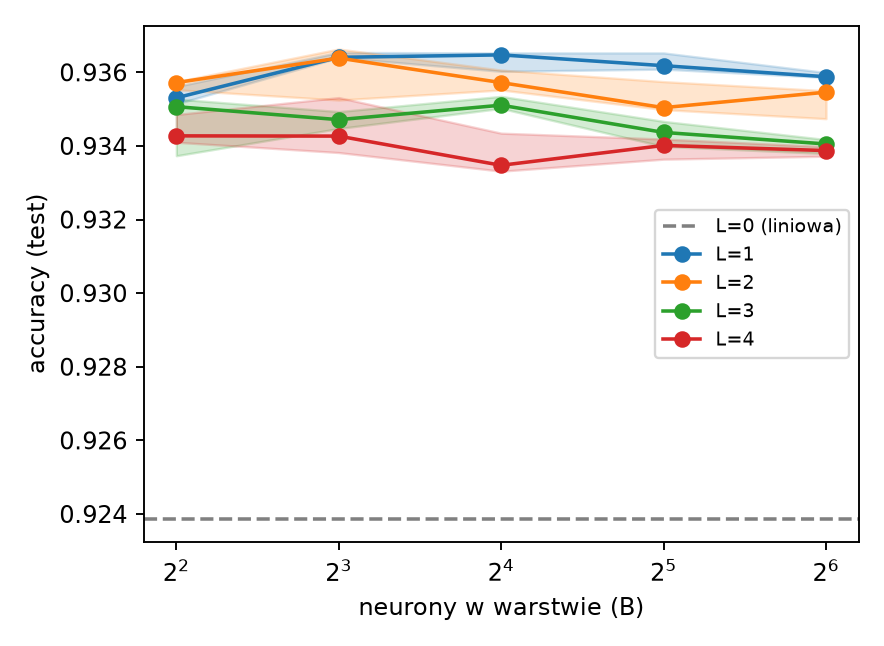
\includegraphics[width=0.7\linewidth]{figures/three_gauss/arch_lines_test_accuracy.png}
  \caption{three\_gauss: accuracy (test) w zależności od $B$ dla każdej liczby warstw $L$ (mediana i kwartyle po ziarnach).}
  \label{fig:three_gauss:arch_lines_test_accuracy}
\end{figure}

\begin{figure}[htbp]
  \centering
  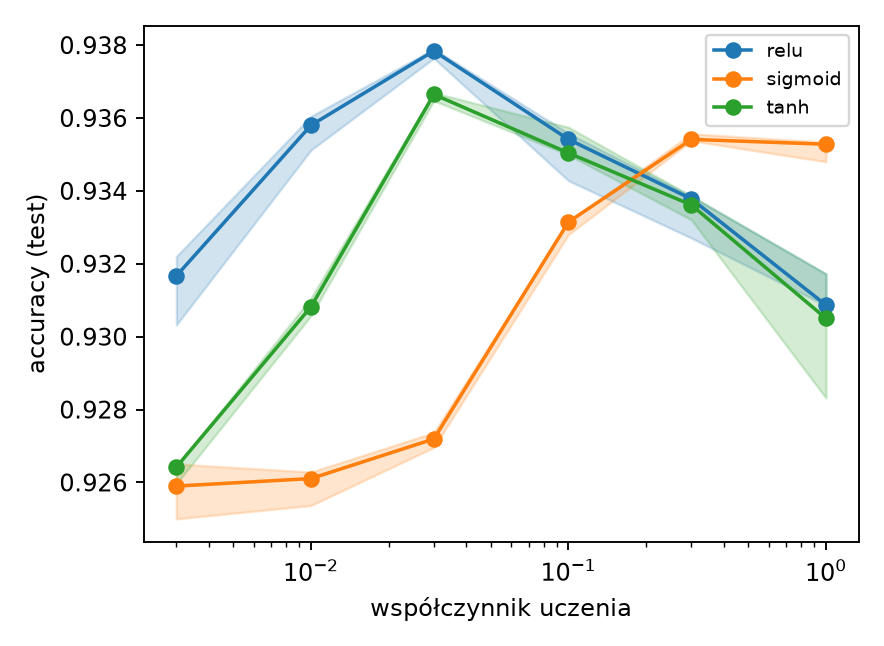
\includegraphics[width=0.7\linewidth]{figures/three_gauss/activation_lr_test_accuracy.png}
  \caption{three\_gauss: accuracy (test) dla różnych funkcji aktywacji w zależności od współczynnika uczenia (mediana i kwartyle; liczba przy krzyżyku nad wykresem to liczba rozbieżnych ziaren).}
  \label{fig:three_gauss:activation_lr_test_accuracy}
\end{figure}

\begin{figure}[htbp]
  \centering
  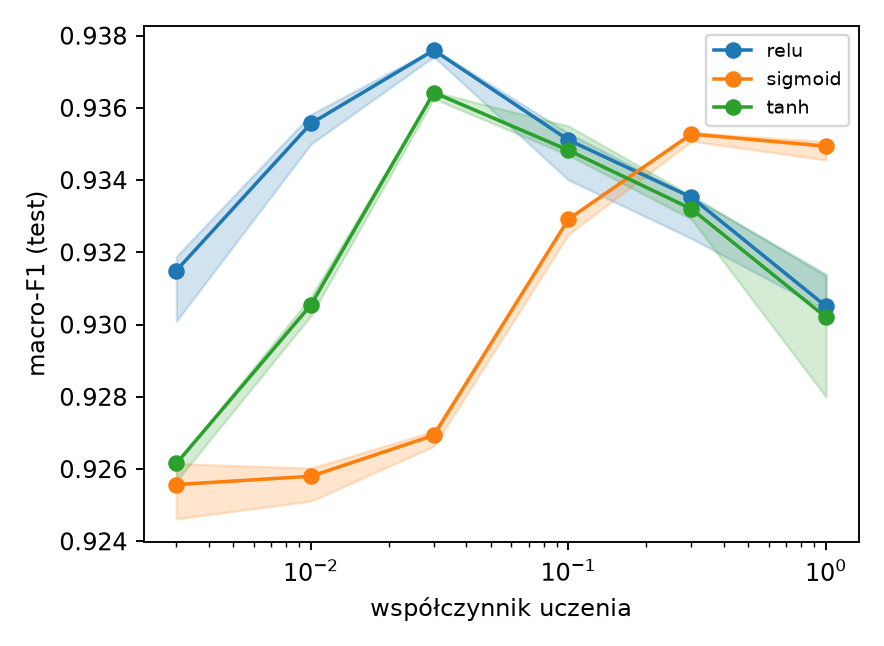
\includegraphics[width=0.7\linewidth]{figures/three_gauss/activation_lr_test_macro_f1.png}
  \caption{three\_gauss: macro-F1 (test) dla różnych funkcji aktywacji w zależności od współczynnika uczenia (mediana i kwartyle; liczba przy krzyżyku nad wykresem to liczba rozbieżnych ziaren).}
  \label{fig:three_gauss:activation_lr_test_macro_f1}
\end{figure}

\begin{figure}[htbp]
  \centering
  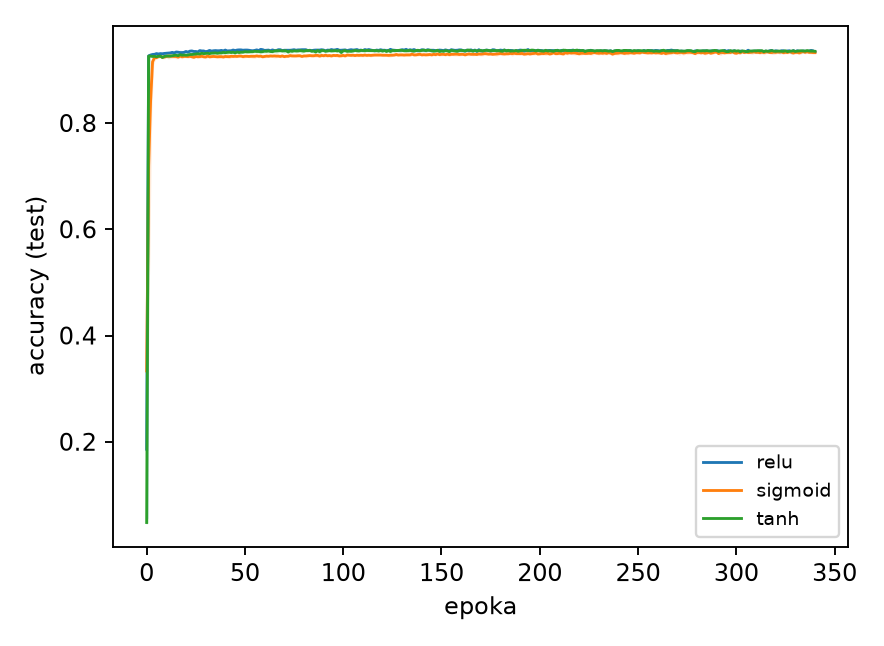
\includegraphics[width=0.7\linewidth]{figures/three_gauss/activation_curve_test_accuracy.png}
  \caption{three\_gauss: przebieg accuracy (test) w trakcie uczenia dla różnych funkcji aktywacji (współczynnik uczenia 0.1).}
  \label{fig:three_gauss:activation_curve_test_accuracy}
\end{figure}

\begin{figure}[htbp]
  \centering
  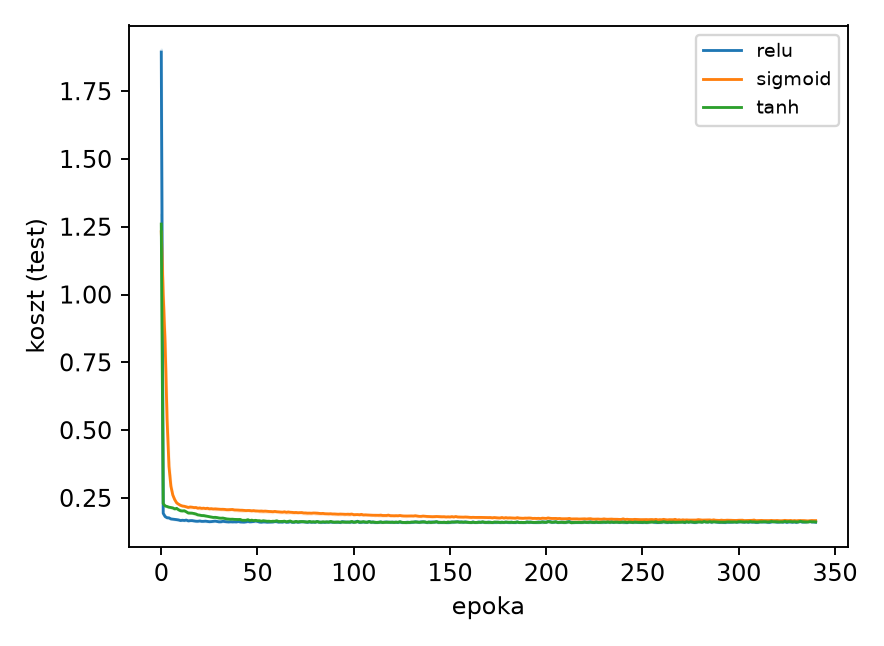
\includegraphics[width=0.7\linewidth]{figures/three_gauss/activation_curve_test_cost.png}
  \caption{three\_gauss: przebieg koszt (test) w trakcie uczenia dla różnych funkcji aktywacji (współczynnik uczenia 0.1).}
  \label{fig:three_gauss:activation_curve_test_cost}
\end{figure}

\begin{figure}[htbp]
  \centering
  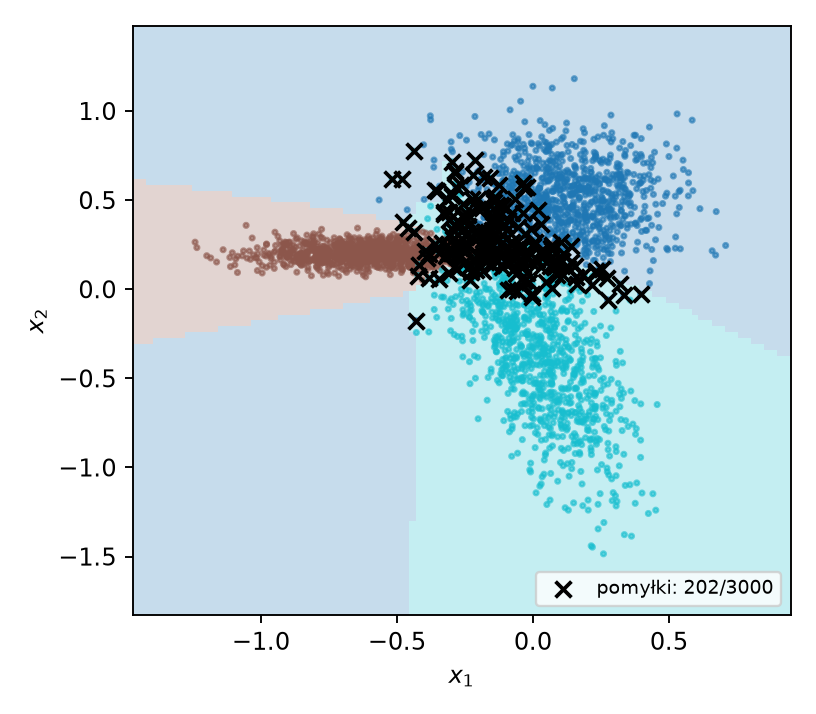
\includegraphics[width=0.7\linewidth]{figures/three_gauss/predictions_relu.png}
  \caption{three\_gauss: obszary decyzyjne sieci z aktywacją relu (ziarno 0). Punkty testowe w kolorze prawdziwej klasy, × oznacza pomyłkę (accuracy 0.933).}
  \label{fig:three_gauss:predictions_relu}
\end{figure}

\begin{figure}[htbp]
  \centering
  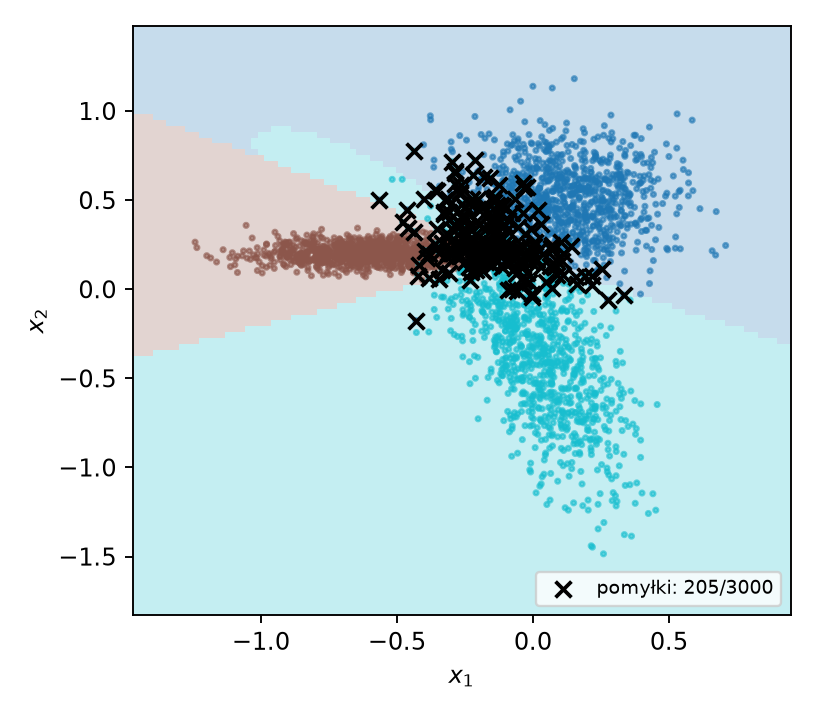
\includegraphics[width=0.7\linewidth]{figures/three_gauss/predictions_sigmoid.png}
  \caption{three\_gauss: obszary decyzyjne sieci z aktywacją sigmoid (ziarno 0). Punkty testowe w kolorze prawdziwej klasy, × oznacza pomyłkę (accuracy 0.932).}
  \label{fig:three_gauss:predictions_sigmoid}
\end{figure}

\begin{figure}[htbp]
  \centering
  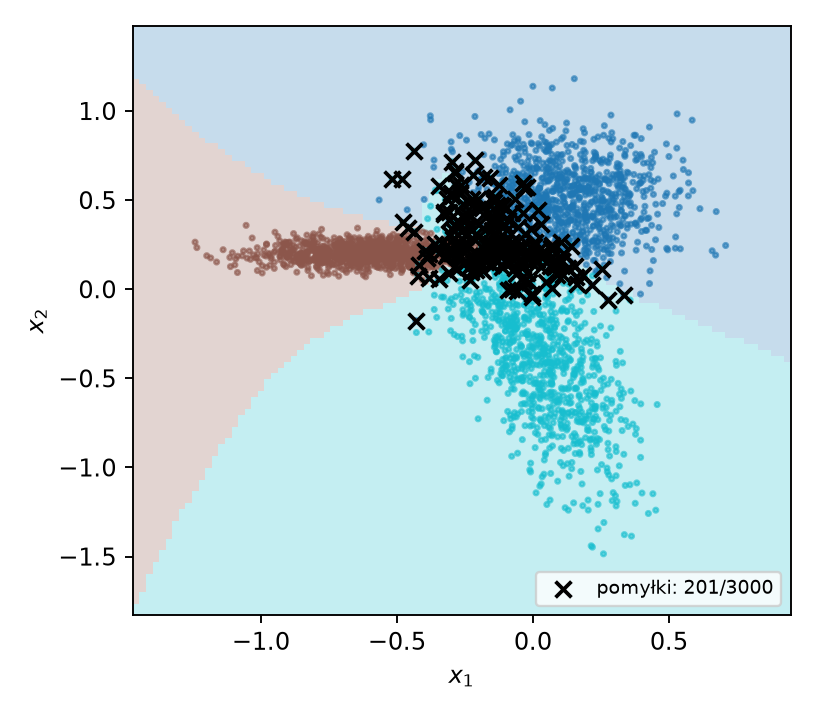
\includegraphics[width=0.7\linewidth]{figures/three_gauss/predictions_tanh.png}
  \caption{three\_gauss: obszary decyzyjne sieci z aktywacją tanh (ziarno 0). Punkty testowe w kolorze prawdziwej klasy, × oznacza pomyłkę (accuracy 0.933).}
  \label{fig:three_gauss:predictions_tanh}
\end{figure}

\begin{figure}[htbp]
  \centering
  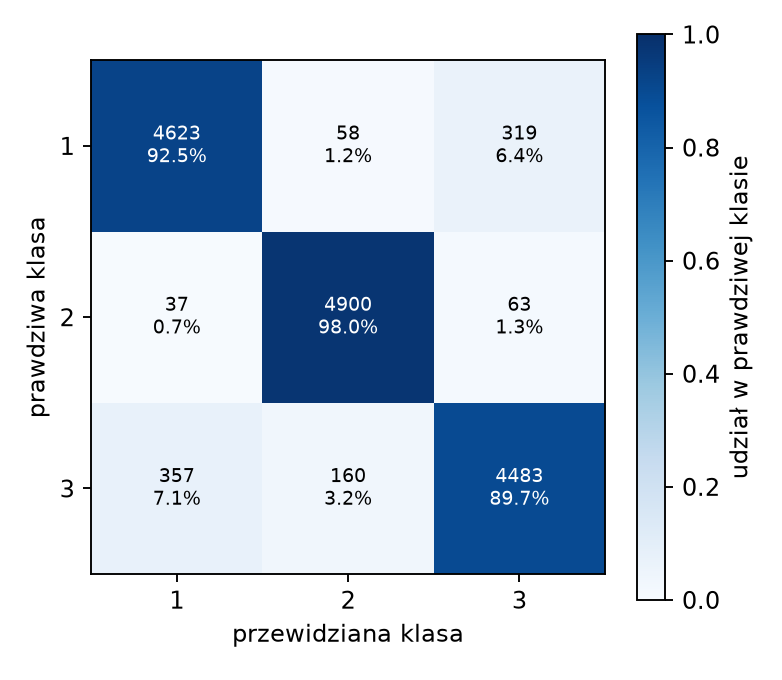
\includegraphics[width=0.7\linewidth]{figures/three_gauss/confusion_relu_32x32.png}
  \caption{three\_gauss: macierz pomyłek na zbiorze testowym, aktywacja relu, architektura 32x32, suma po 5 ziarnach (accuracy 0.934).}
  \label{fig:three_gauss:confusion_relu_32x32}
\end{figure}

\begin{figure}[htbp]
  \centering
  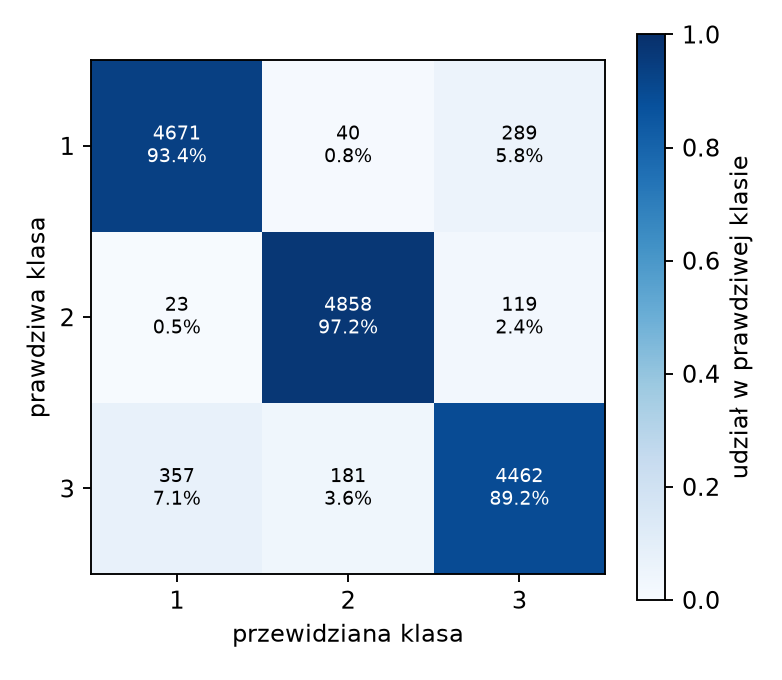
\includegraphics[width=0.7\linewidth]{figures/three_gauss/confusion_sigmoid_32x32.png}
  \caption{three\_gauss: macierz pomyłek na zbiorze testowym, aktywacja sigmoid, architektura 32x32, suma po 5 ziarnach (accuracy 0.933).}
  \label{fig:three_gauss:confusion_sigmoid_32x32}
\end{figure}

\begin{figure}[htbp]
  \centering
  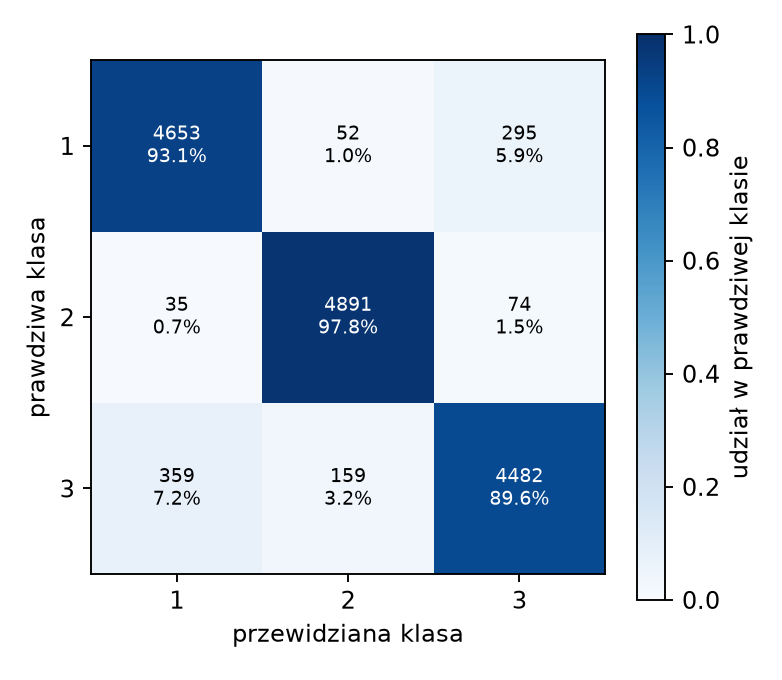
\includegraphics[width=0.7\linewidth]{figures/three_gauss/confusion_tanh_32x32.png}
  \caption{three\_gauss: macierz pomyłek na zbiorze testowym, aktywacja tanh, architektura 32x32, suma po 5 ziarnach (accuracy 0.935).}
  \label{fig:three_gauss:confusion_tanh_32x32}
\end{figure}

\begin{figure}[htbp]
  \centering
  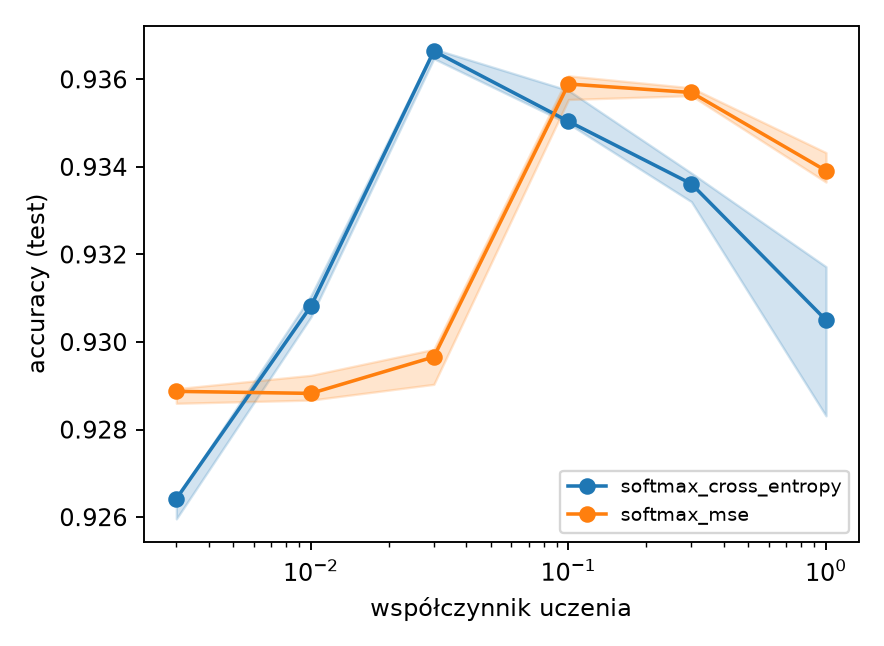
\includegraphics[width=0.7\linewidth]{figures/three_gauss/loss_lr_test_accuracy.png}
  \caption{three\_gauss: accuracy (test) dla różnych funkcji kosztu w zależności od współczynnika uczenia (mediana i kwartyle; liczba przy krzyżyku nad wykresem to liczba rozbieżnych ziaren).}
  \label{fig:three_gauss:loss_lr_test_accuracy}
\end{figure}

\begin{figure}[htbp]
  \centering
  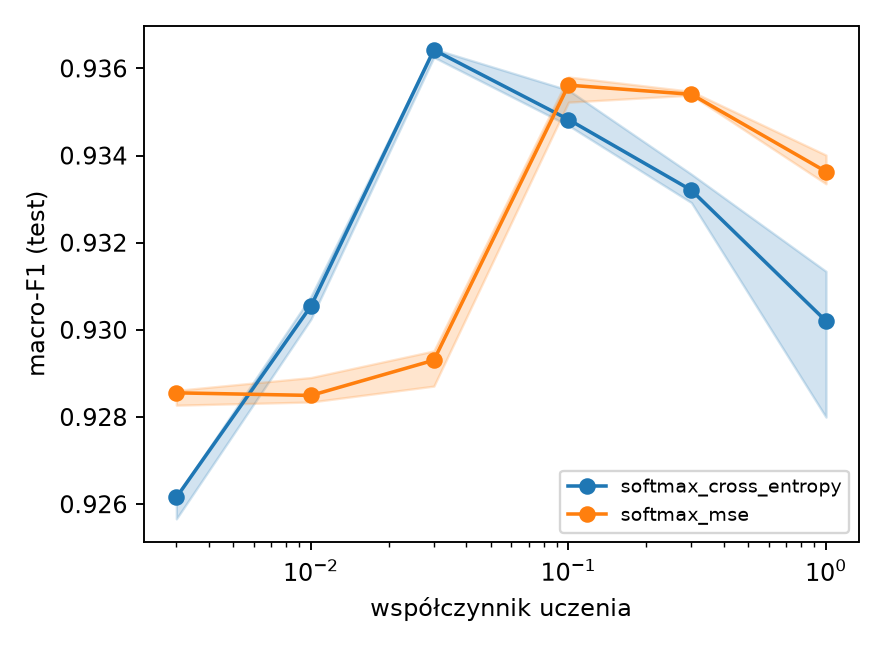
\includegraphics[width=0.7\linewidth]{figures/three_gauss/loss_lr_test_macro_f1.png}
  \caption{three\_gauss: macro-F1 (test) dla różnych funkcji kosztu w zależności od współczynnika uczenia (mediana i kwartyle; liczba przy krzyżyku nad wykresem to liczba rozbieżnych ziaren).}
  \label{fig:three_gauss:loss_lr_test_macro_f1}
\end{figure}

\begin{figure}[htbp]
  \centering
  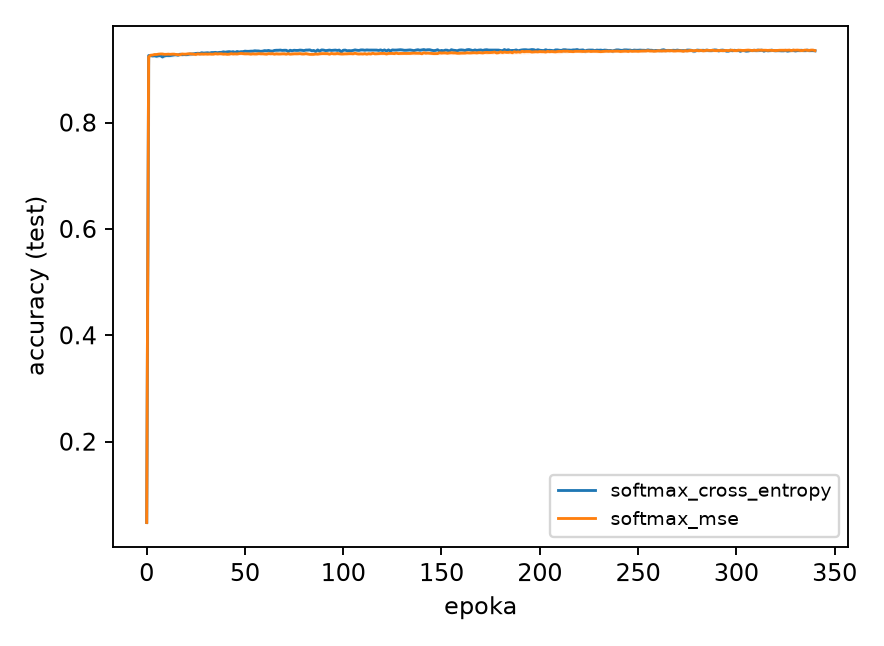
\includegraphics[width=0.7\linewidth]{figures/three_gauss/loss_curve_test_accuracy.png}
  \caption{three\_gauss: przebieg accuracy (test) w trakcie uczenia dla różnych funkcji kosztu (współczynnik uczenia 0.1).}
  \label{fig:three_gauss:loss_curve_test_accuracy}
\end{figure}

\begin{figure}[htbp]
  \centering
  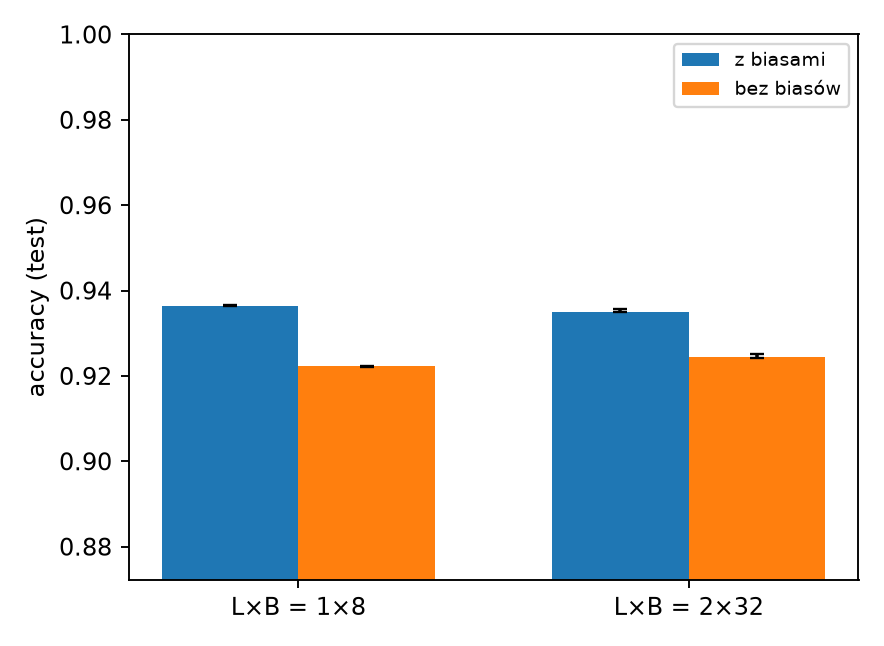
\includegraphics[width=0.7\linewidth]{figures/three_gauss/bias.png}
  \caption{three\_gauss: accuracy (test) sieci z biasami i bez biasów.}
  \label{fig:three_gauss:bias}
\end{figure}

\begin{figure}[htbp]
  \centering
  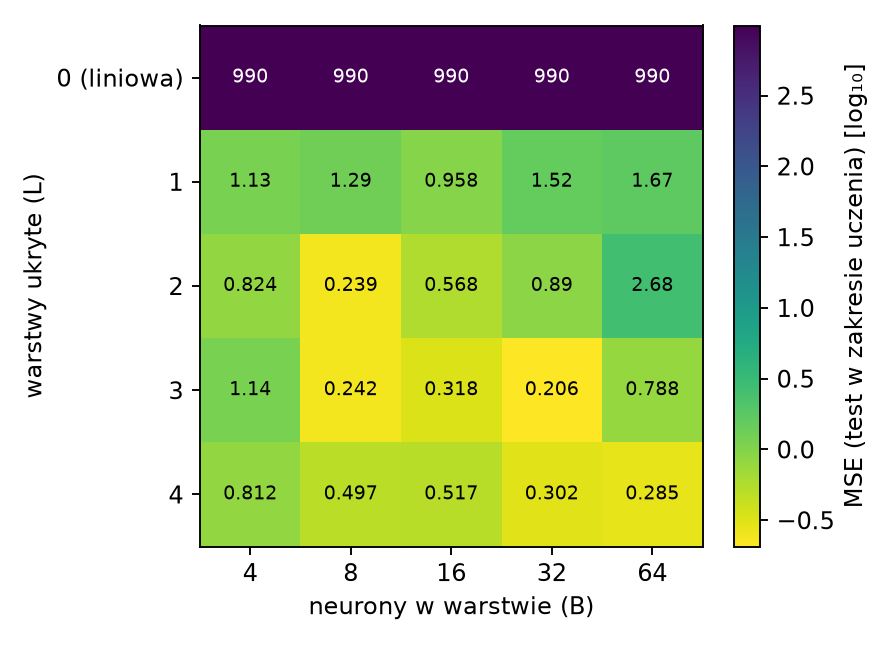
\includegraphics[width=0.7\linewidth]{figures/cube/arch_heatmap_test_in_mse.png}
  \caption{cube: MSE (test w zakresie uczenia) (mediana) w zależności od liczby warstw ukrytych $L$ i neuronów w warstwie $B$.}
  \label{fig:cube:arch_heatmap_test_in_mse}
\end{figure}

\begin{figure}[htbp]
  \centering
  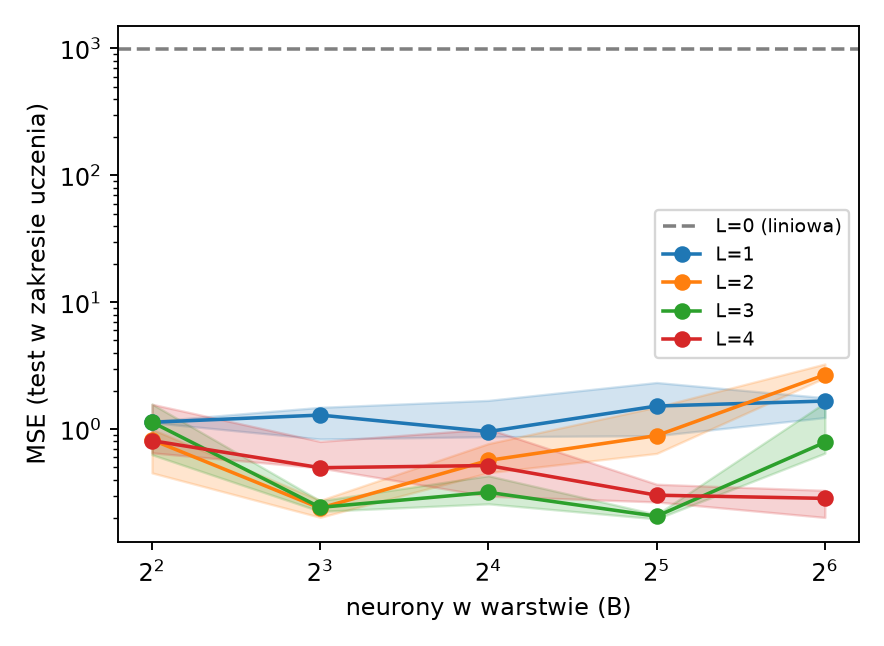
\includegraphics[width=0.7\linewidth]{figures/cube/arch_lines_test_in_mse.png}
  \caption{cube: MSE (test w zakresie uczenia) w zależności od $B$ dla każdej liczby warstw $L$ (mediana i kwartyle po ziarnach).}
  \label{fig:cube:arch_lines_test_in_mse}
\end{figure}

\begin{figure}[htbp]
  \centering
  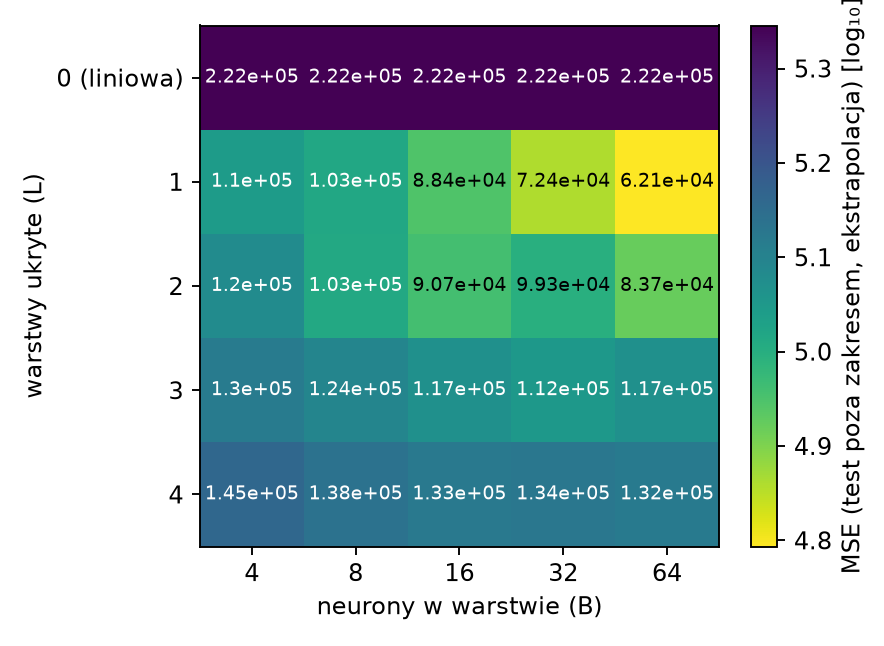
\includegraphics[width=0.7\linewidth]{figures/cube/arch_heatmap_test_out_mse.png}
  \caption{cube: MSE (test poza zakresem, ekstrapolacja) (mediana) w zależności od liczby warstw ukrytych $L$ i neuronów w warstwie $B$.}
  \label{fig:cube:arch_heatmap_test_out_mse}
\end{figure}

\begin{figure}[htbp]
  \centering
  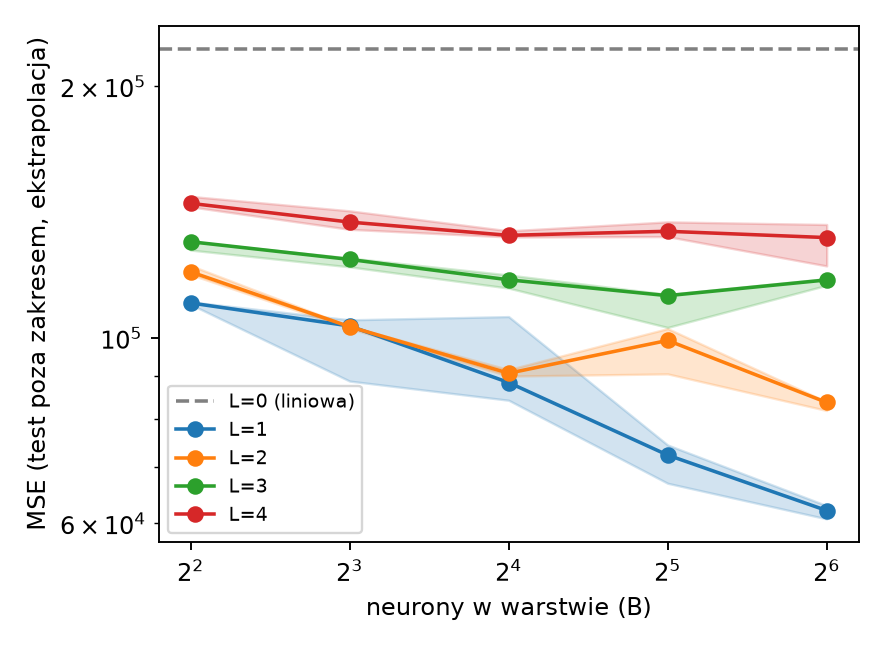
\includegraphics[width=0.7\linewidth]{figures/cube/arch_lines_test_out_mse.png}
  \caption{cube: MSE (test poza zakresem, ekstrapolacja) w zależności od $B$ dla każdej liczby warstw $L$ (mediana i kwartyle po ziarnach).}
  \label{fig:cube:arch_lines_test_out_mse}
\end{figure}

\begin{figure}[htbp]
  \centering
  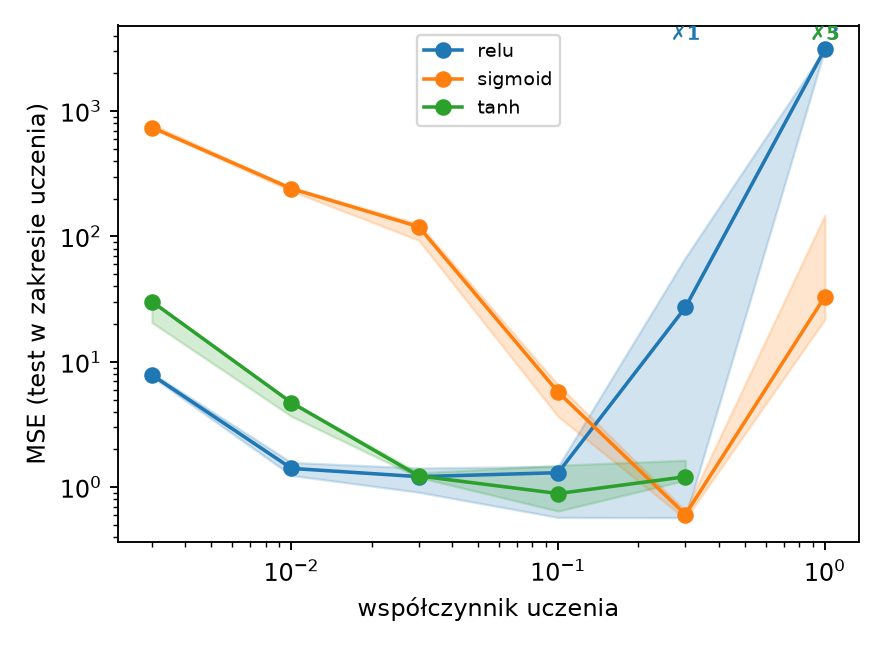
\includegraphics[width=0.7\linewidth]{figures/cube/activation_lr_test_in_mse.png}
  \caption{cube: MSE (test w zakresie uczenia) dla różnych funkcji aktywacji w zależności od współczynnika uczenia (mediana i kwartyle; liczba przy krzyżyku nad wykresem to liczba rozbieżnych ziaren).}
  \label{fig:cube:activation_lr_test_in_mse}
\end{figure}

\begin{figure}[htbp]
  \centering
  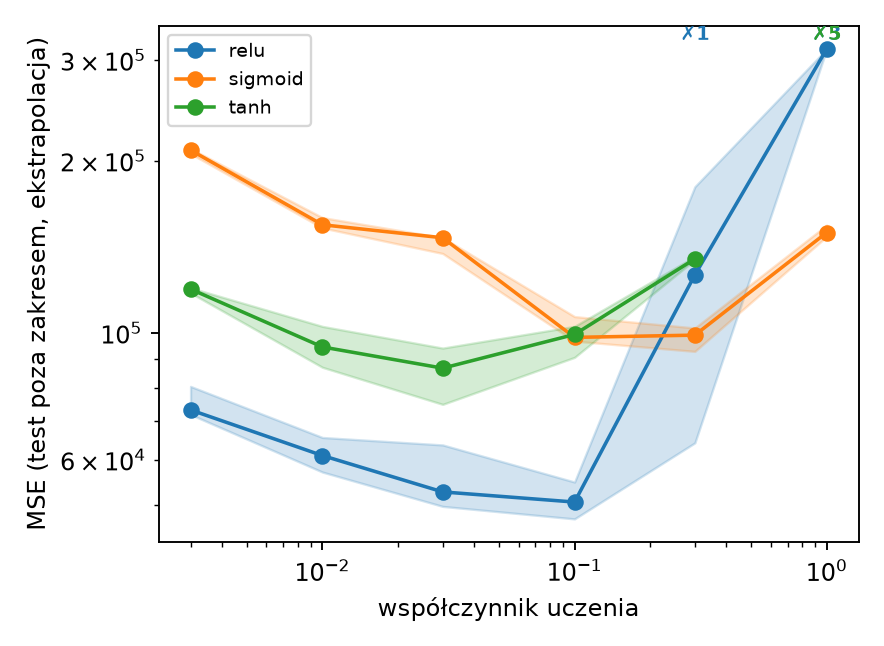
\includegraphics[width=0.7\linewidth]{figures/cube/activation_lr_test_out_mse.png}
  \caption{cube: MSE (test poza zakresem, ekstrapolacja) dla różnych funkcji aktywacji w zależności od współczynnika uczenia (mediana i kwartyle; liczba przy krzyżyku nad wykresem to liczba rozbieżnych ziaren).}
  \label{fig:cube:activation_lr_test_out_mse}
\end{figure}

\begin{figure}[htbp]
  \centering
  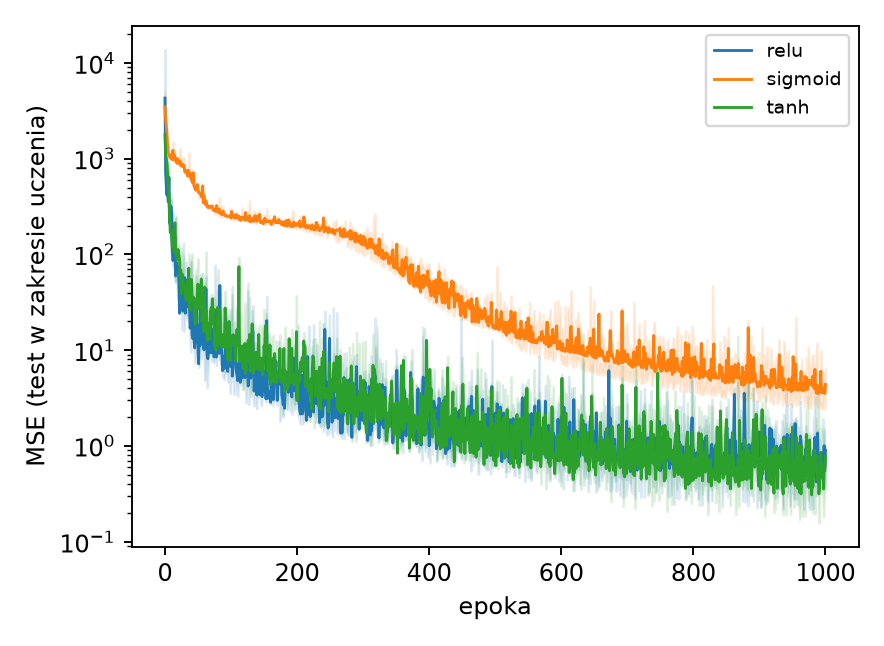
\includegraphics[width=0.7\linewidth]{figures/cube/activation_curve_test_in_mse.png}
  \caption{cube: przebieg MSE (test w zakresie uczenia) w trakcie uczenia dla różnych funkcji aktywacji (współczynnik uczenia 0.1).}
  \label{fig:cube:activation_curve_test_in_mse}
\end{figure}

\begin{figure}[htbp]
  \centering
  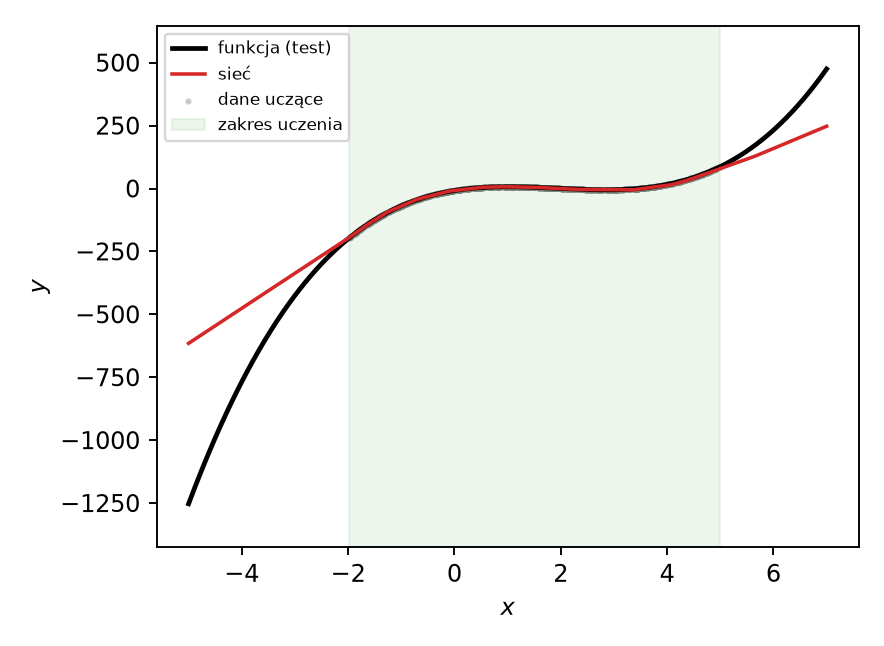
\includegraphics[width=0.7\linewidth]{figures/cube/predictions_relu.png}
  \caption{cube: funkcja nauczona przez sieć z aktywacją relu (ziarno 0) na całym zakresie testu; zielone tło to zakres danych uczących.}
  \label{fig:cube:predictions_relu}
\end{figure}

\begin{figure}[htbp]
  \centering
  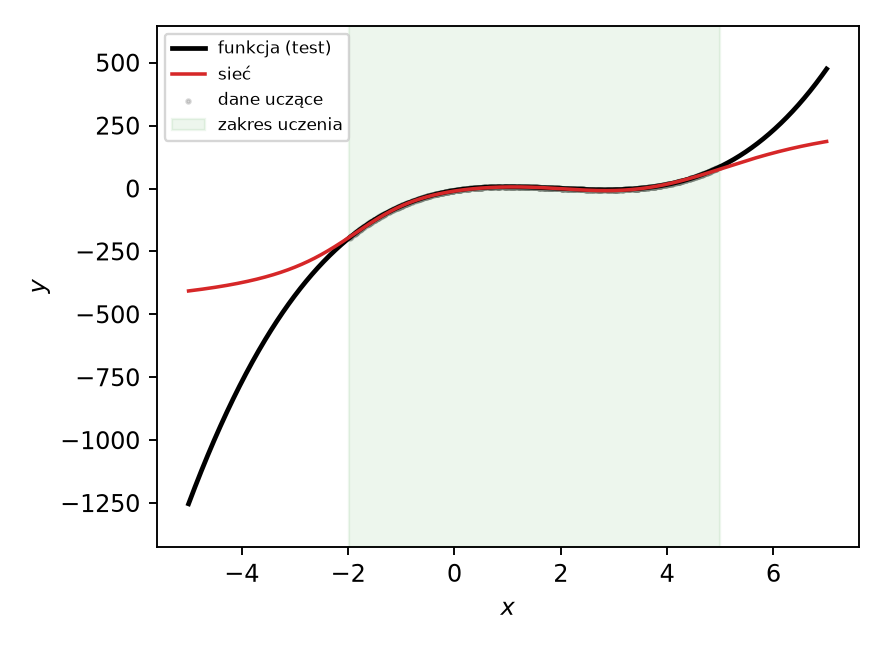
\includegraphics[width=0.7\linewidth]{figures/cube/predictions_sigmoid.png}
  \caption{cube: funkcja nauczona przez sieć z aktywacją sigmoid (ziarno 0) na całym zakresie testu; zielone tło to zakres danych uczących.}
  \label{fig:cube:predictions_sigmoid}
\end{figure}

\begin{figure}[htbp]
  \centering
  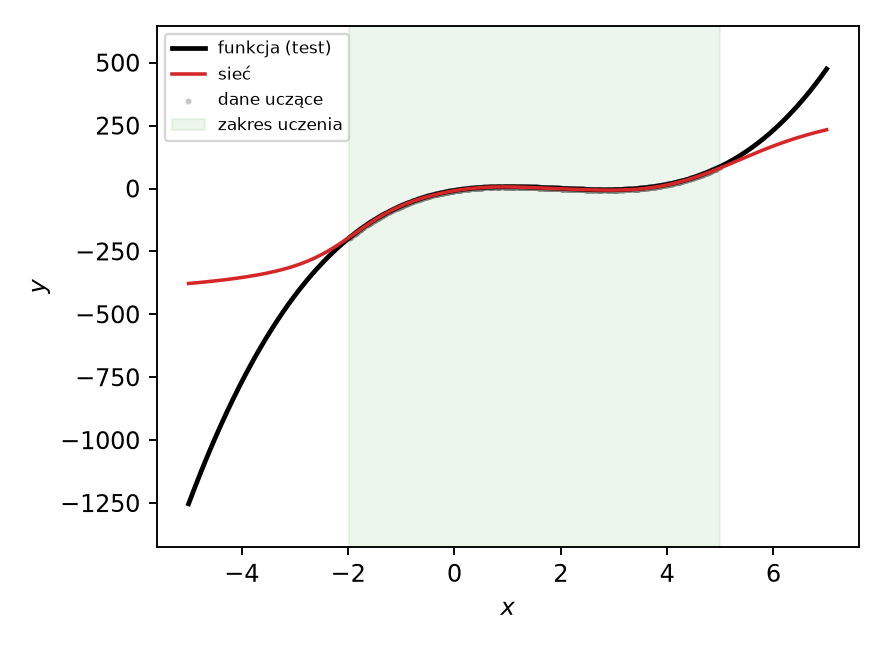
\includegraphics[width=0.7\linewidth]{figures/cube/predictions_tanh.png}
  \caption{cube: funkcja nauczona przez sieć z aktywacją tanh (ziarno 0) na całym zakresie testu; zielone tło to zakres danych uczących.}
  \label{fig:cube:predictions_tanh}
\end{figure}

\begin{figure}[htbp]
  \centering
  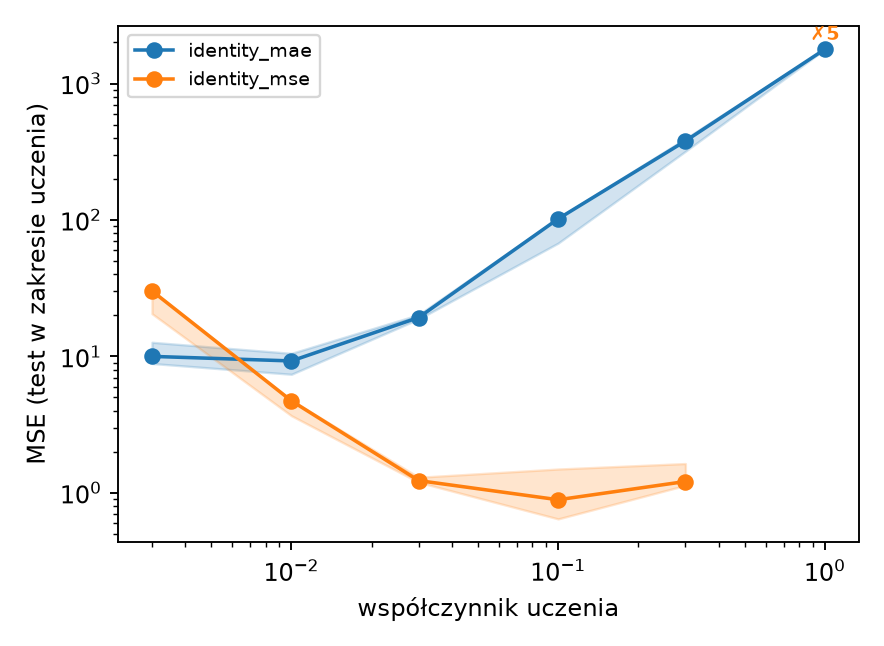
\includegraphics[width=0.7\linewidth]{figures/cube/loss_lr_test_in_mse.png}
  \caption{cube: MSE (test w zakresie uczenia) dla różnych funkcji kosztu w zależności od współczynnika uczenia (mediana i kwartyle; liczba przy krzyżyku nad wykresem to liczba rozbieżnych ziaren).}
  \label{fig:cube:loss_lr_test_in_mse}
\end{figure}

\begin{figure}[htbp]
  \centering
  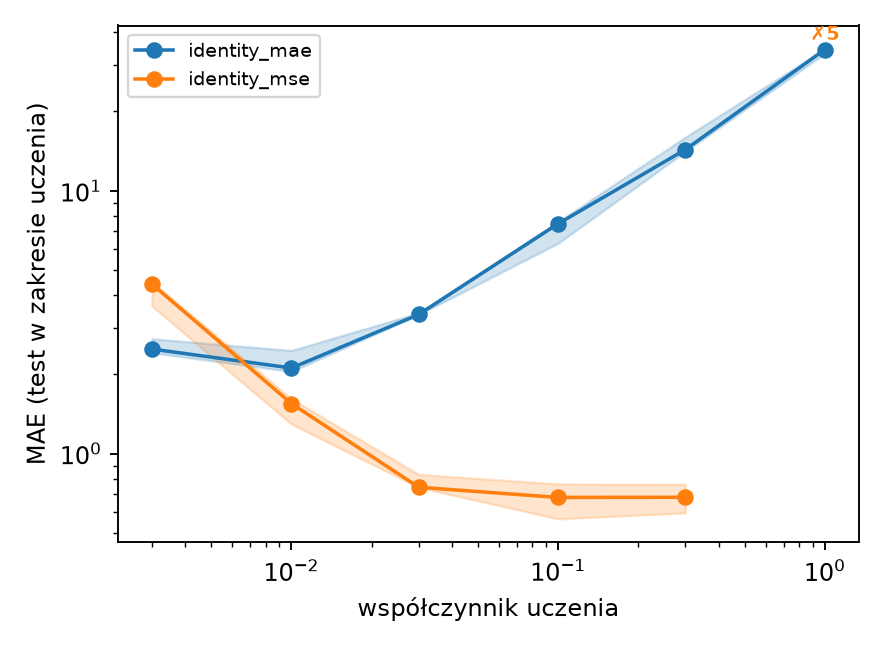
\includegraphics[width=0.7\linewidth]{figures/cube/loss_lr_test_in_mae.png}
  \caption{cube: MAE (test w zakresie uczenia) dla różnych funkcji kosztu w zależności od współczynnika uczenia (mediana i kwartyle; liczba przy krzyżyku nad wykresem to liczba rozbieżnych ziaren).}
  \label{fig:cube:loss_lr_test_in_mae}
\end{figure}

\begin{figure}[htbp]
  \centering
  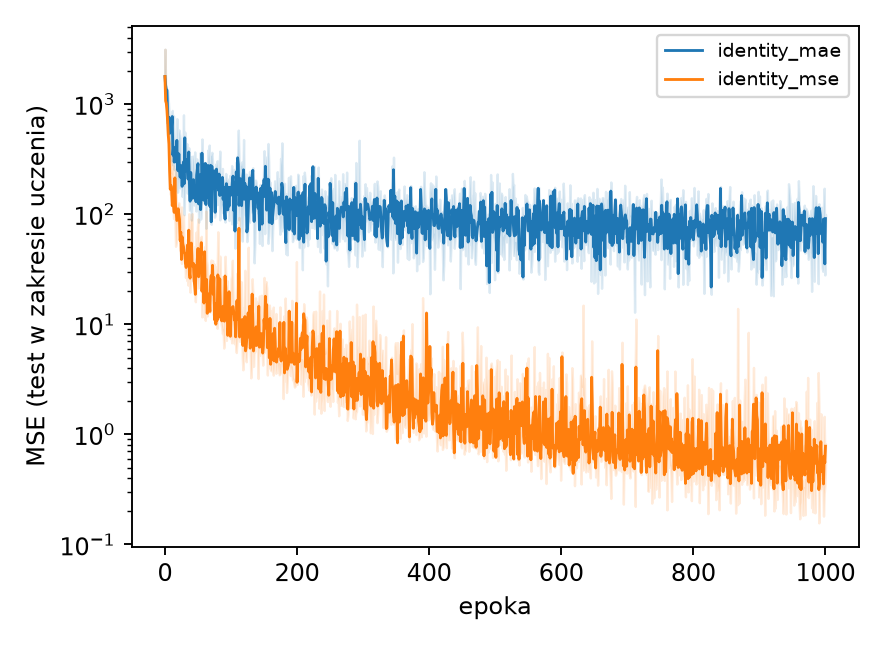
\includegraphics[width=0.7\linewidth]{figures/cube/loss_curve_test_in_mse.png}
  \caption{cube: przebieg MSE (test w zakresie uczenia) w trakcie uczenia dla różnych funkcji kosztu (współczynnik uczenia 0.1).}
  \label{fig:cube:loss_curve_test_in_mse}
\end{figure}

\begin{figure}[htbp]
  \centering
  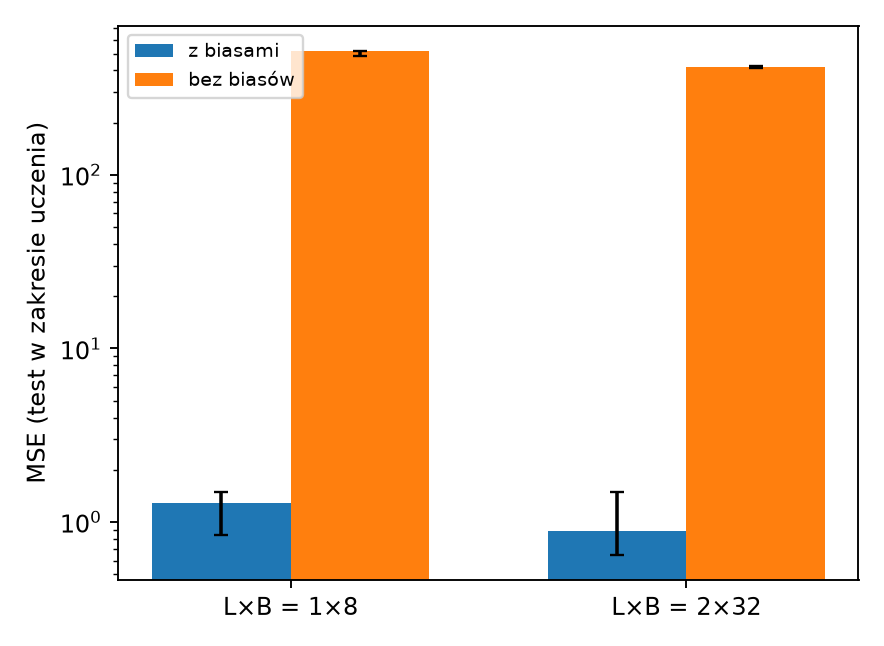
\includegraphics[width=0.7\linewidth]{figures/cube/bias.png}
  \caption{cube: MSE (test w zakresie uczenia) sieci z biasami i bez biasów.}
  \label{fig:cube:bias}
\end{figure}

\begin{figure}[htbp]
  \centering
  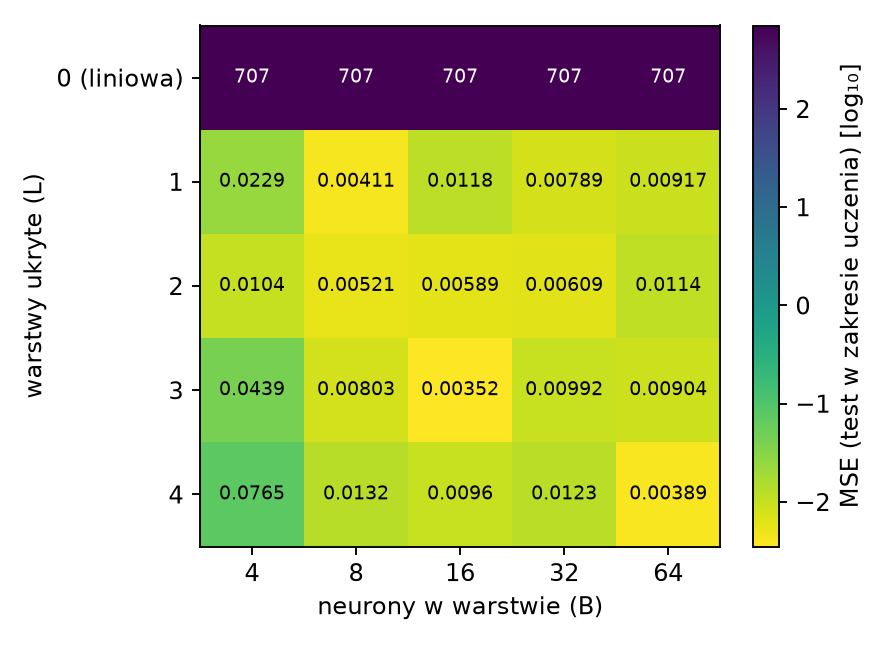
\includegraphics[width=0.7\linewidth]{figures/activation/arch_heatmap_test_in_mse.png}
  \caption{activation: MSE (test w zakresie uczenia) (mediana) w zależności od liczby warstw ukrytych $L$ i neuronów w warstwie $B$.}
  \label{fig:activation:arch_heatmap_test_in_mse}
\end{figure}

\begin{figure}[htbp]
  \centering
  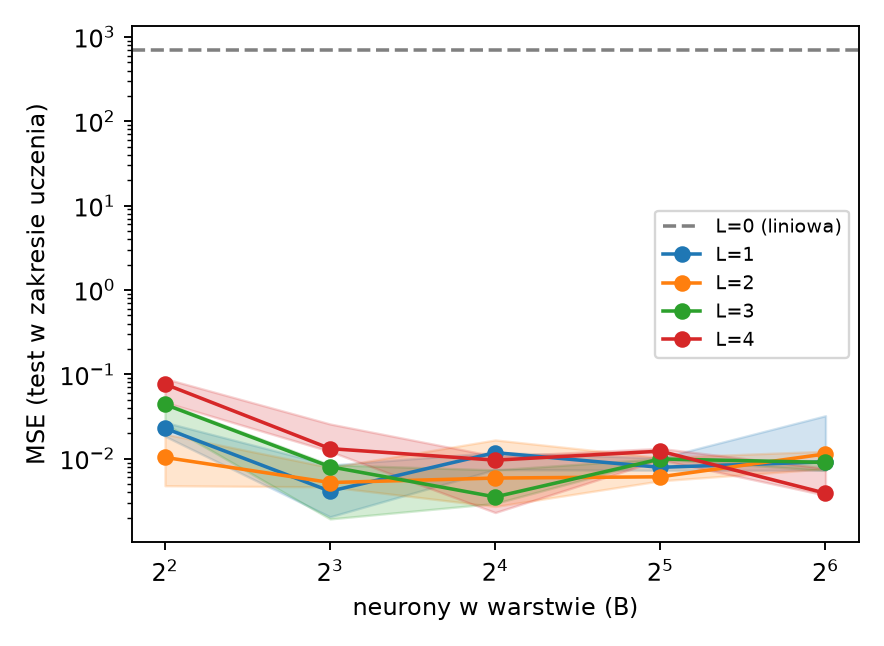
\includegraphics[width=0.7\linewidth]{figures/activation/arch_lines_test_in_mse.png}
  \caption{activation: MSE (test w zakresie uczenia) w zależności od $B$ dla każdej liczby warstw $L$ (mediana i kwartyle po ziarnach).}
  \label{fig:activation:arch_lines_test_in_mse}
\end{figure}

\begin{figure}[htbp]
  \centering
  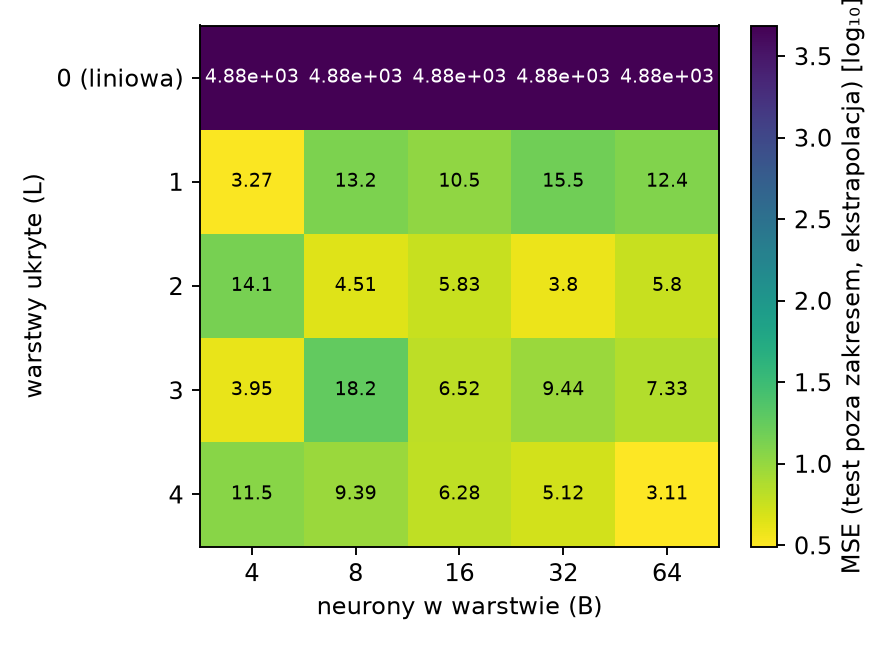
\includegraphics[width=0.7\linewidth]{figures/activation/arch_heatmap_test_out_mse.png}
  \caption{activation: MSE (test poza zakresem, ekstrapolacja) (mediana) w zależności od liczby warstw ukrytych $L$ i neuronów w warstwie $B$.}
  \label{fig:activation:arch_heatmap_test_out_mse}
\end{figure}

\begin{figure}[htbp]
  \centering
  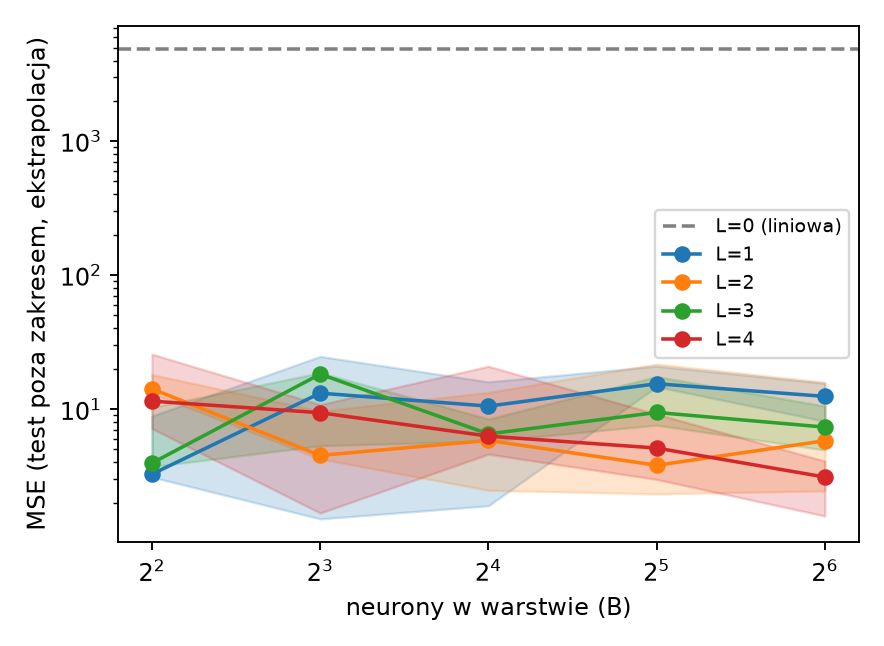
\includegraphics[width=0.7\linewidth]{figures/activation/arch_lines_test_out_mse.png}
  \caption{activation: MSE (test poza zakresem, ekstrapolacja) w zależności od $B$ dla każdej liczby warstw $L$ (mediana i kwartyle po ziarnach).}
  \label{fig:activation:arch_lines_test_out_mse}
\end{figure}

\begin{figure}[htbp]
  \centering
  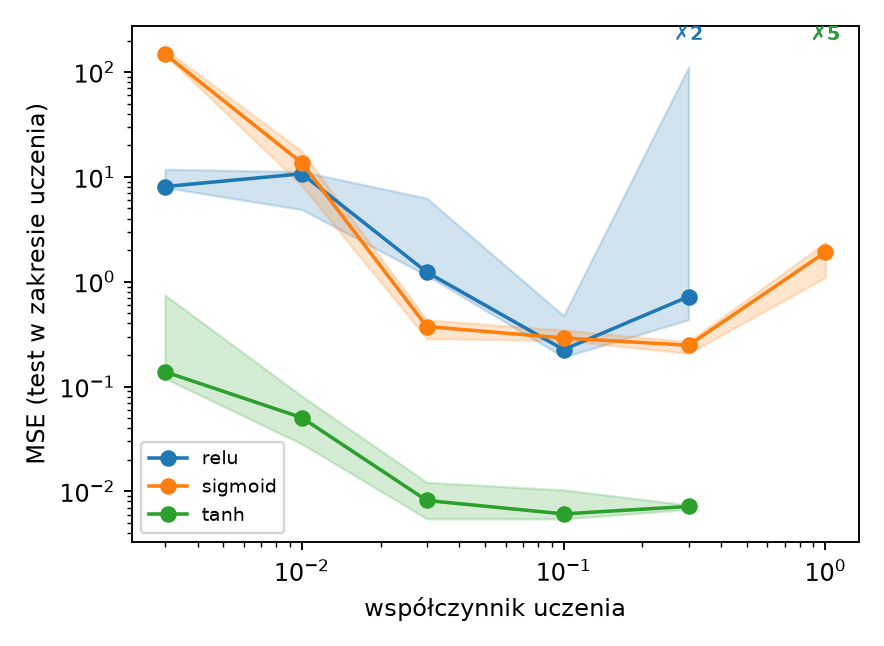
\includegraphics[width=0.7\linewidth]{figures/activation/activation_lr_test_in_mse.png}
  \caption{activation: MSE (test w zakresie uczenia) dla różnych funkcji aktywacji w zależności od współczynnika uczenia (mediana i kwartyle; liczba przy krzyżyku nad wykresem to liczba rozbieżnych ziaren).}
  \label{fig:activation:activation_lr_test_in_mse}
\end{figure}

\begin{figure}[htbp]
  \centering
  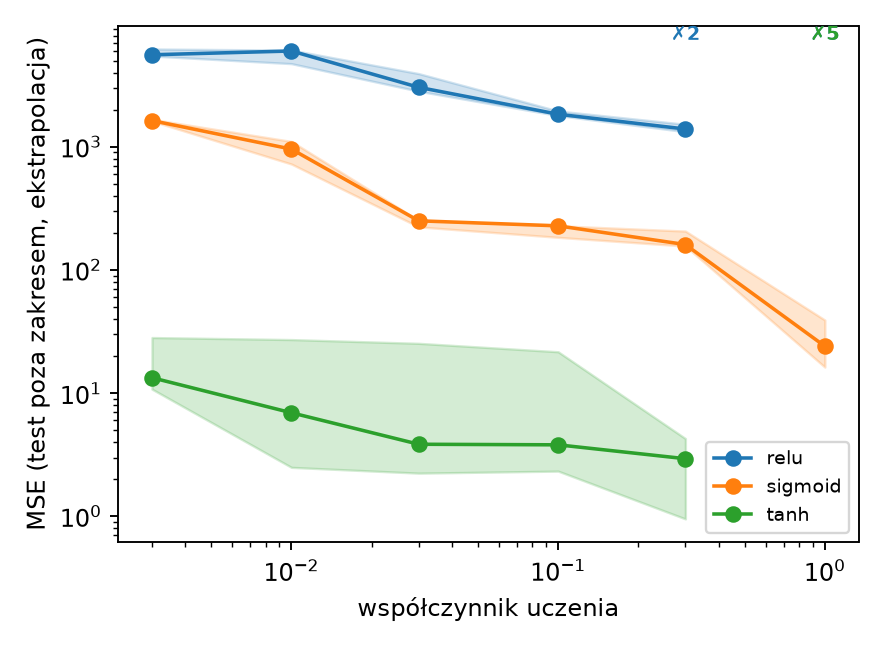
\includegraphics[width=0.7\linewidth]{figures/activation/activation_lr_test_out_mse.png}
  \caption{activation: MSE (test poza zakresem, ekstrapolacja) dla różnych funkcji aktywacji w zależności od współczynnika uczenia (mediana i kwartyle; liczba przy krzyżyku nad wykresem to liczba rozbieżnych ziaren).}
  \label{fig:activation:activation_lr_test_out_mse}
\end{figure}

\begin{figure}[htbp]
  \centering
  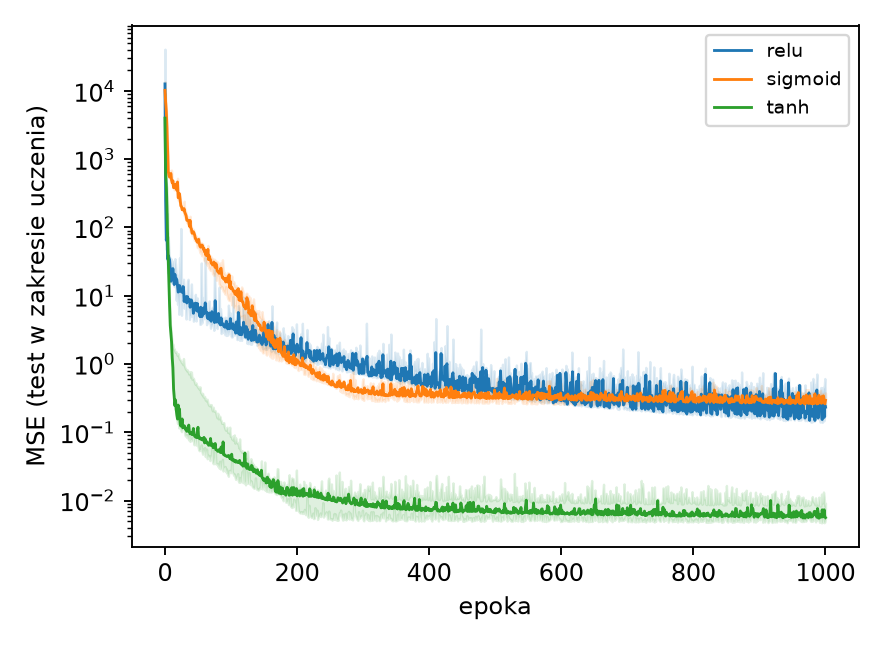
\includegraphics[width=0.7\linewidth]{figures/activation/activation_curve_test_in_mse.png}
  \caption{activation: przebieg MSE (test w zakresie uczenia) w trakcie uczenia dla różnych funkcji aktywacji (współczynnik uczenia 0.1).}
  \label{fig:activation:activation_curve_test_in_mse}
\end{figure}

\begin{figure}[htbp]
  \centering
  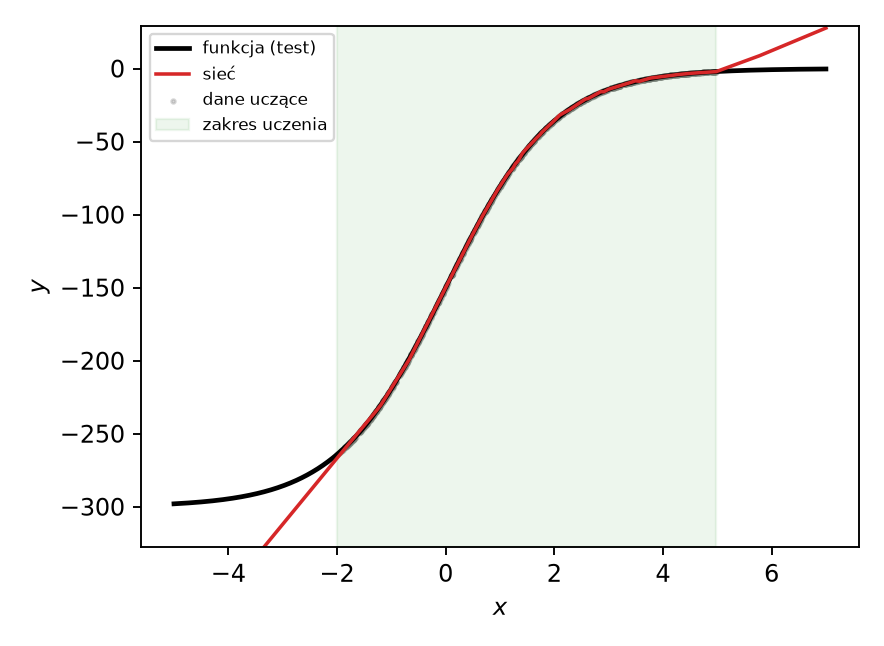
\includegraphics[width=0.7\linewidth]{figures/activation/predictions_relu.png}
  \caption{activation: funkcja nauczona przez sieć z aktywacją relu (ziarno 0) na całym zakresie testu; zielone tło to zakres danych uczących.}
  \label{fig:activation:predictions_relu}
\end{figure}

\begin{figure}[htbp]
  \centering
  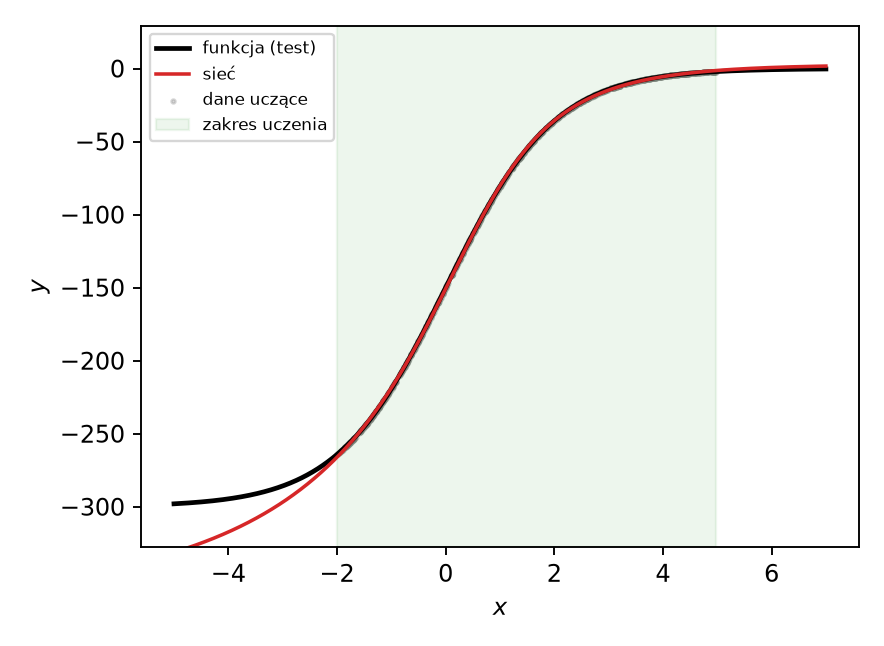
\includegraphics[width=0.7\linewidth]{figures/activation/predictions_sigmoid.png}
  \caption{activation: funkcja nauczona przez sieć z aktywacją sigmoid (ziarno 0) na całym zakresie testu; zielone tło to zakres danych uczących.}
  \label{fig:activation:predictions_sigmoid}
\end{figure}

\begin{figure}[htbp]
  \centering
  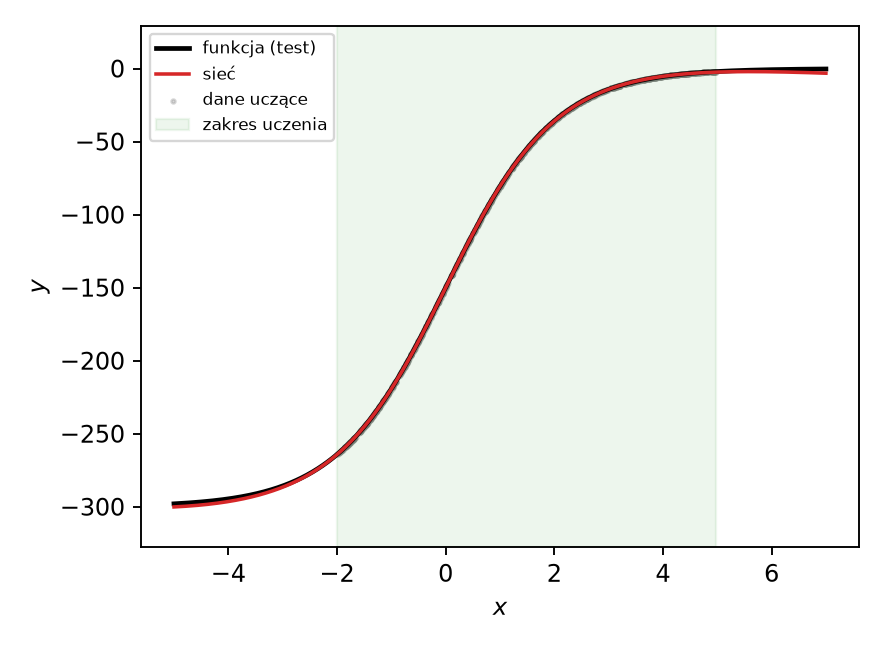
\includegraphics[width=0.7\linewidth]{figures/activation/predictions_tanh.png}
  \caption{activation: funkcja nauczona przez sieć z aktywacją tanh (ziarno 0) na całym zakresie testu; zielone tło to zakres danych uczących.}
  \label{fig:activation:predictions_tanh}
\end{figure}

\begin{figure}[htbp]
  \centering
  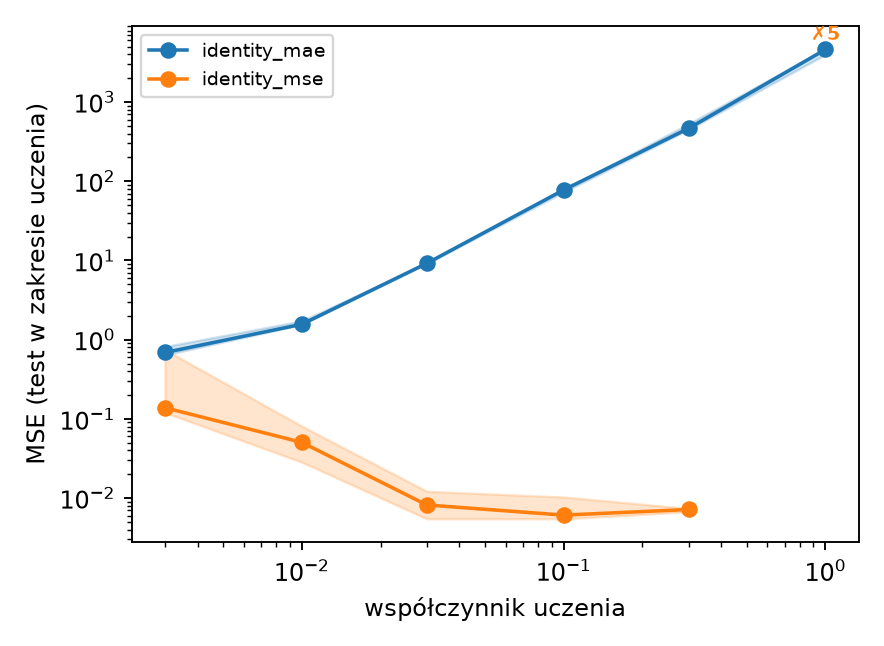
\includegraphics[width=0.7\linewidth]{figures/activation/loss_lr_test_in_mse.png}
  \caption{activation: MSE (test w zakresie uczenia) dla różnych funkcji kosztu w zależności od współczynnika uczenia (mediana i kwartyle; liczba przy krzyżyku nad wykresem to liczba rozbieżnych ziaren).}
  \label{fig:activation:loss_lr_test_in_mse}
\end{figure}

\begin{figure}[htbp]
  \centering
  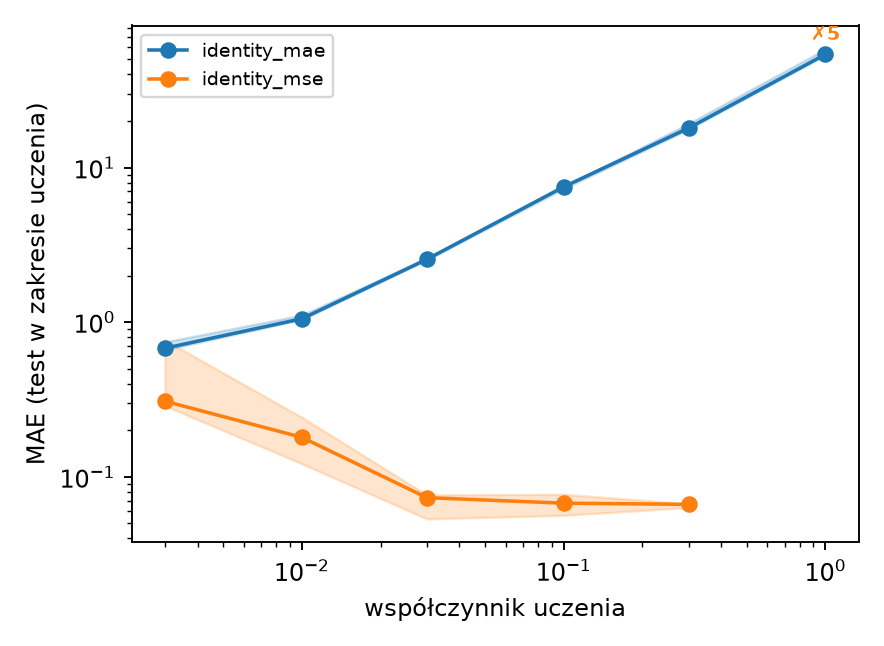
\includegraphics[width=0.7\linewidth]{figures/activation/loss_lr_test_in_mae.png}
  \caption{activation: MAE (test w zakresie uczenia) dla różnych funkcji kosztu w zależności od współczynnika uczenia (mediana i kwartyle; liczba przy krzyżyku nad wykresem to liczba rozbieżnych ziaren).}
  \label{fig:activation:loss_lr_test_in_mae}
\end{figure}

\begin{figure}[htbp]
  \centering
  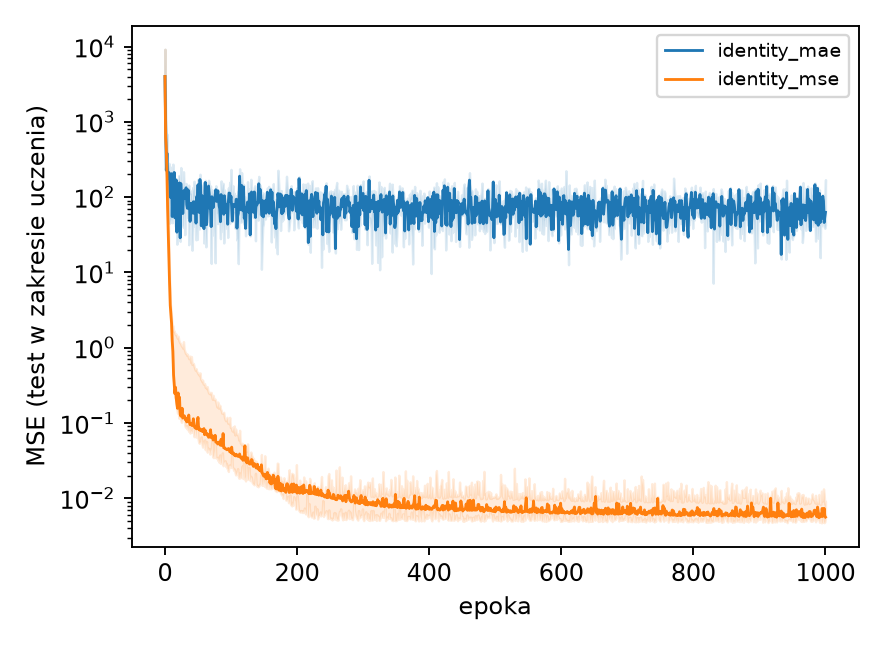
\includegraphics[width=0.7\linewidth]{figures/activation/loss_curve_test_in_mse.png}
  \caption{activation: przebieg MSE (test w zakresie uczenia) w trakcie uczenia dla różnych funkcji kosztu (współczynnik uczenia 0.1).}
  \label{fig:activation:loss_curve_test_in_mse}
\end{figure}

\begin{figure}[htbp]
  \centering
  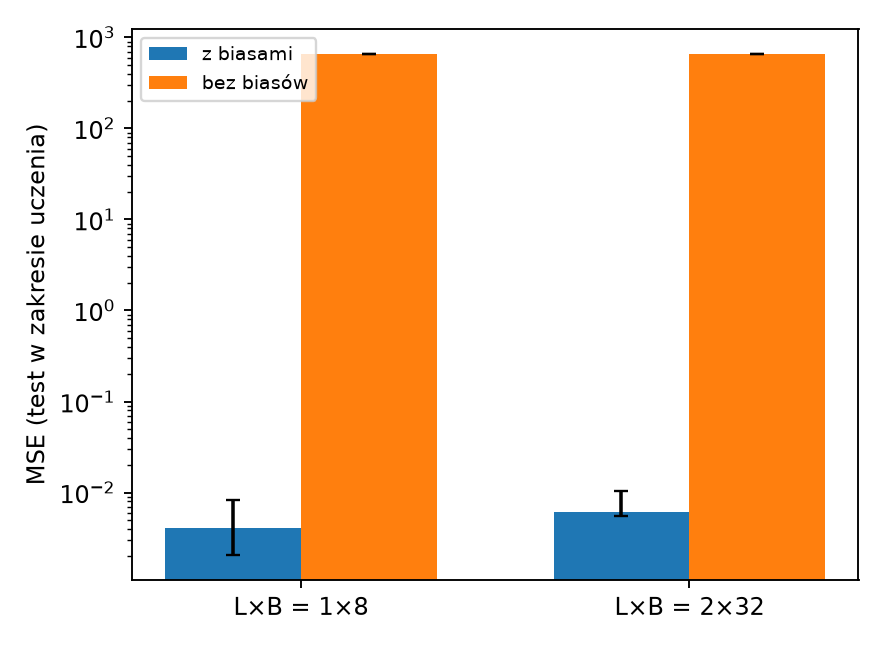
\includegraphics[width=0.7\linewidth]{figures/activation/bias.png}
  \caption{activation: MSE (test w zakresie uczenia) sieci z biasami i bez biasów.}
  \label{fig:activation:bias}
\end{figure}

\begin{figure}[htbp]
  \centering
  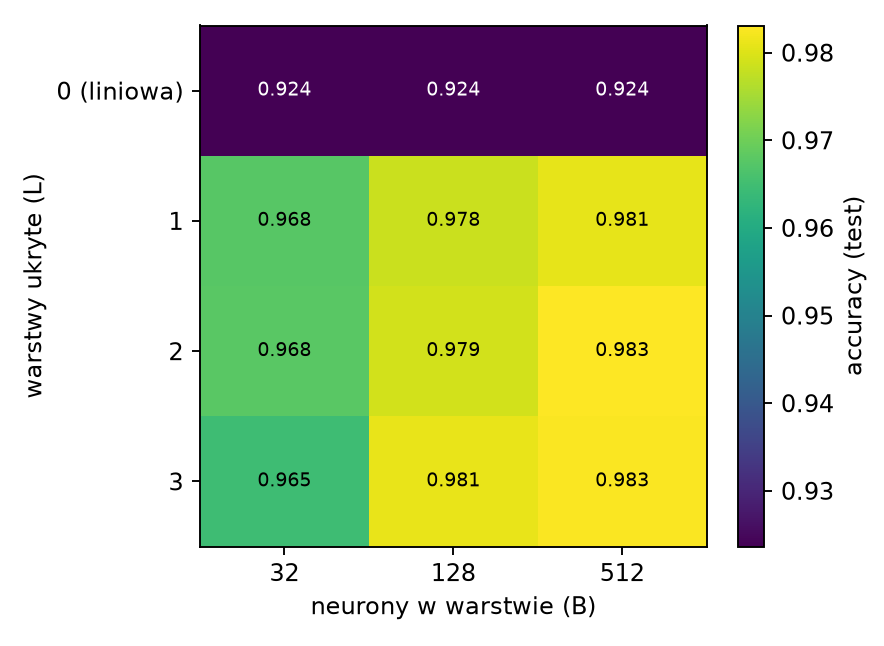
\includegraphics[width=0.7\linewidth]{figures/mnist/arch_heatmap_test_accuracy.png}
  \caption{MNIST: accuracy (test) (mediana) w zależności od liczby warstw ukrytych $L$ i neuronów w warstwie $B$.}
  \label{fig:mnist:arch_heatmap_test_accuracy}
\end{figure}

\begin{figure}[htbp]
  \centering
  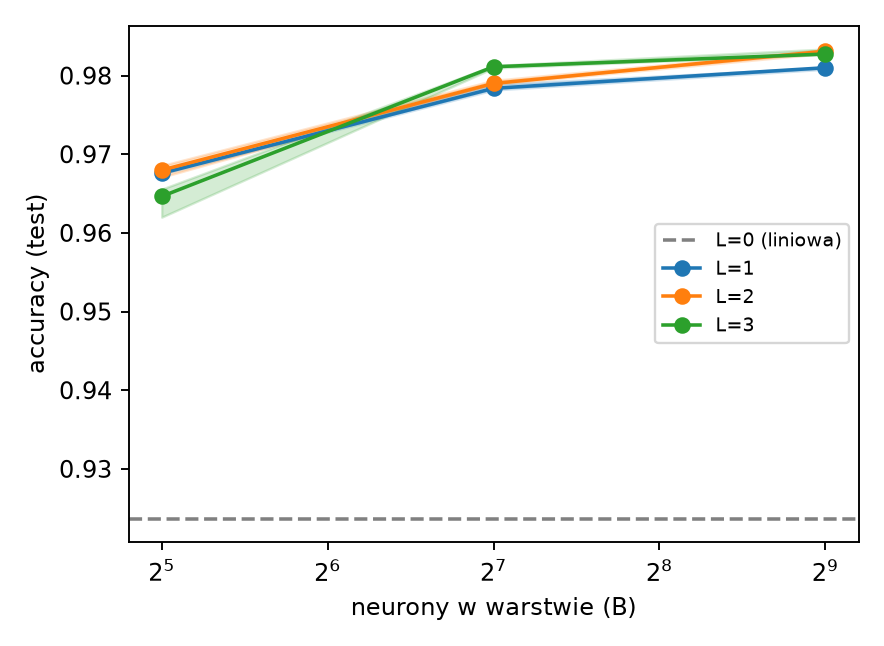
\includegraphics[width=0.7\linewidth]{figures/mnist/arch_lines_test_accuracy.png}
  \caption{MNIST: accuracy (test) w zależności od $B$ dla każdej liczby warstw $L$ (mediana i kwartyle po ziarnach).}
  \label{fig:mnist:arch_lines_test_accuracy}
\end{figure}

\begin{figure}[htbp]
  \centering
  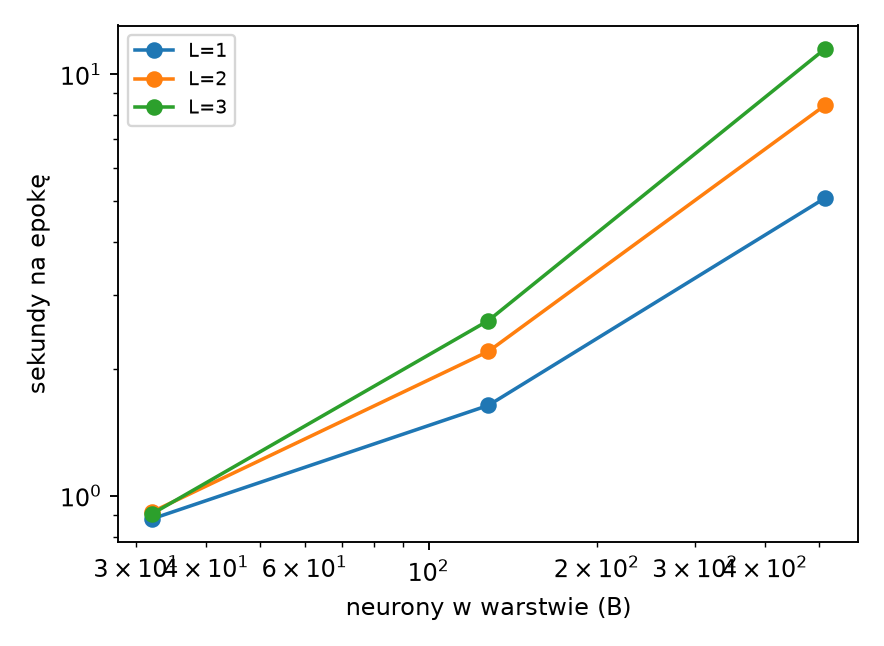
\includegraphics[width=0.7\linewidth]{figures/mnist/time_per_epoch.png}
  \caption{MNIST: czas jednej epoki (uczenie i ewaluacja, jeden wątek) w zależności od architektury.}
  \label{fig:mnist:time_per_epoch}
\end{figure}

\begin{figure}[htbp]
  \centering
  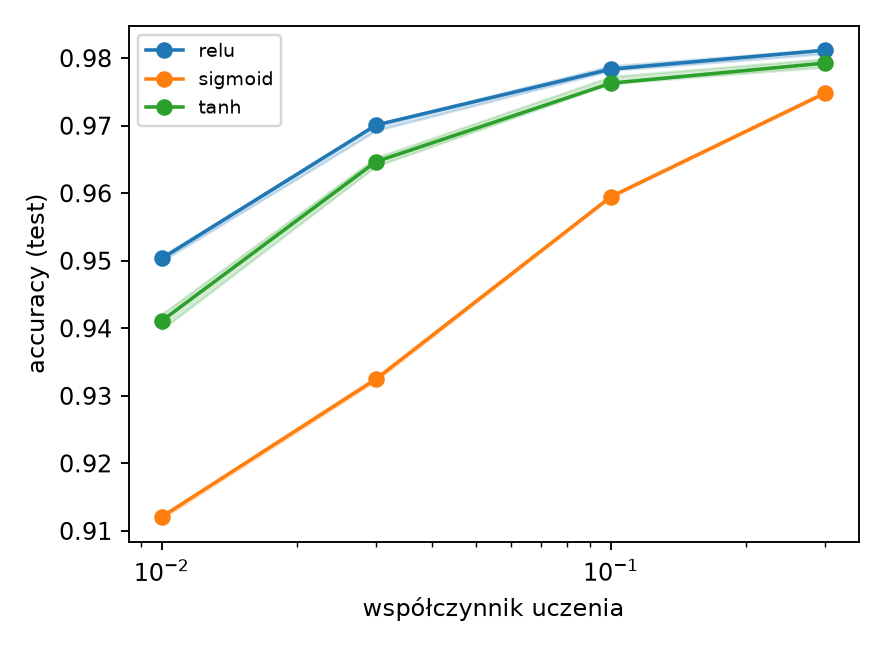
\includegraphics[width=0.7\linewidth]{figures/mnist/activation_lr_test_accuracy.png}
  \caption{MNIST: accuracy (test) dla różnych funkcji aktywacji w zależności od współczynnika uczenia (mediana i kwartyle; liczba przy krzyżyku nad wykresem to liczba rozbieżnych ziaren).}
  \label{fig:mnist:activation_lr_test_accuracy}
\end{figure}

\begin{figure}[htbp]
  \centering
  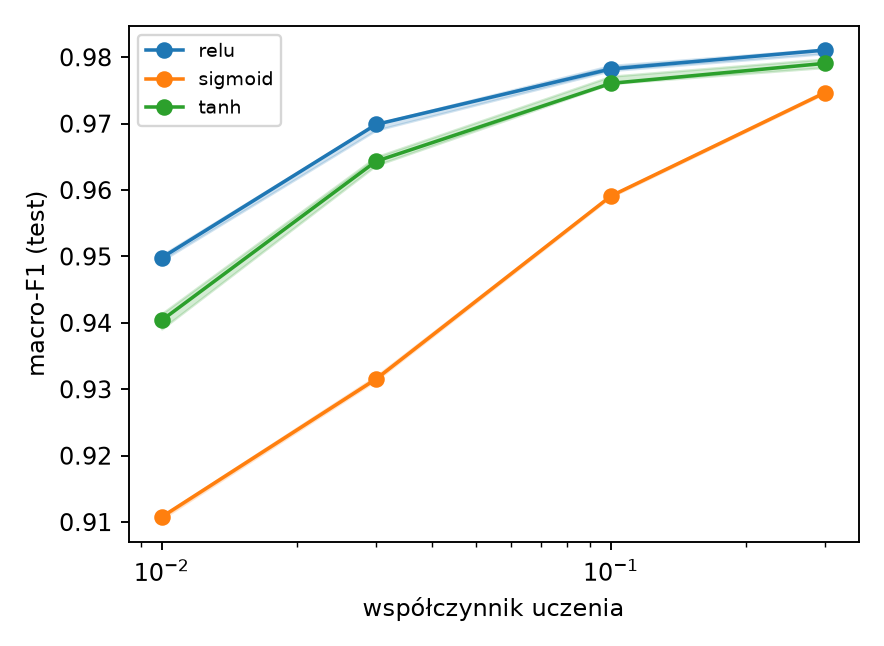
\includegraphics[width=0.7\linewidth]{figures/mnist/activation_lr_test_macro_f1.png}
  \caption{MNIST: macro-F1 (test) dla różnych funkcji aktywacji w zależności od współczynnika uczenia (mediana i kwartyle; liczba przy krzyżyku nad wykresem to liczba rozbieżnych ziaren).}
  \label{fig:mnist:activation_lr_test_macro_f1}
\end{figure}

\begin{figure}[htbp]
  \centering
  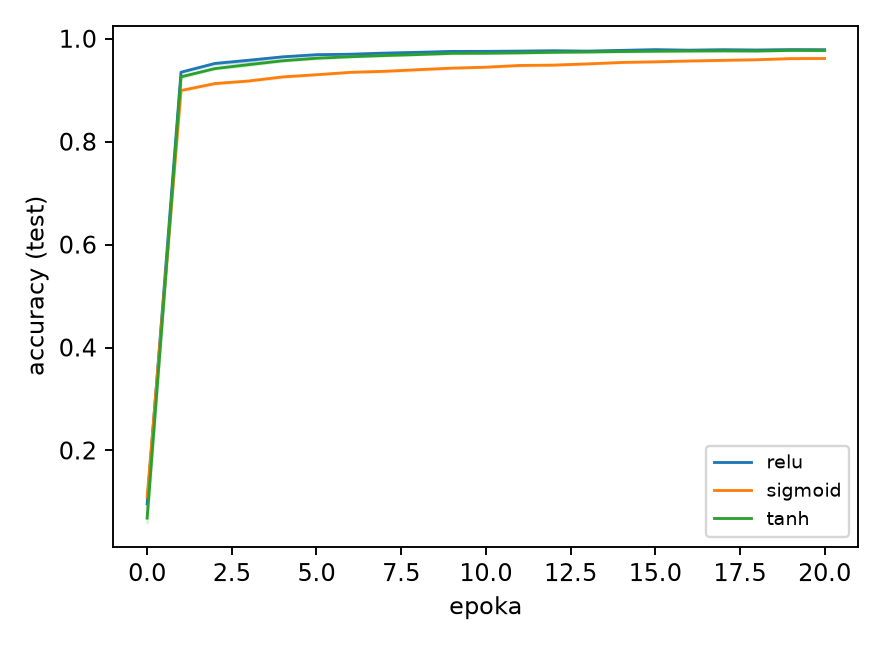
\includegraphics[width=0.7\linewidth]{figures/mnist/activation_curve_test_accuracy.png}
  \caption{MNIST: przebieg accuracy (test) w trakcie uczenia dla różnych funkcji aktywacji (współczynnik uczenia 0.1).}
  \label{fig:mnist:activation_curve_test_accuracy}
\end{figure}

\begin{figure}[htbp]
  \centering
  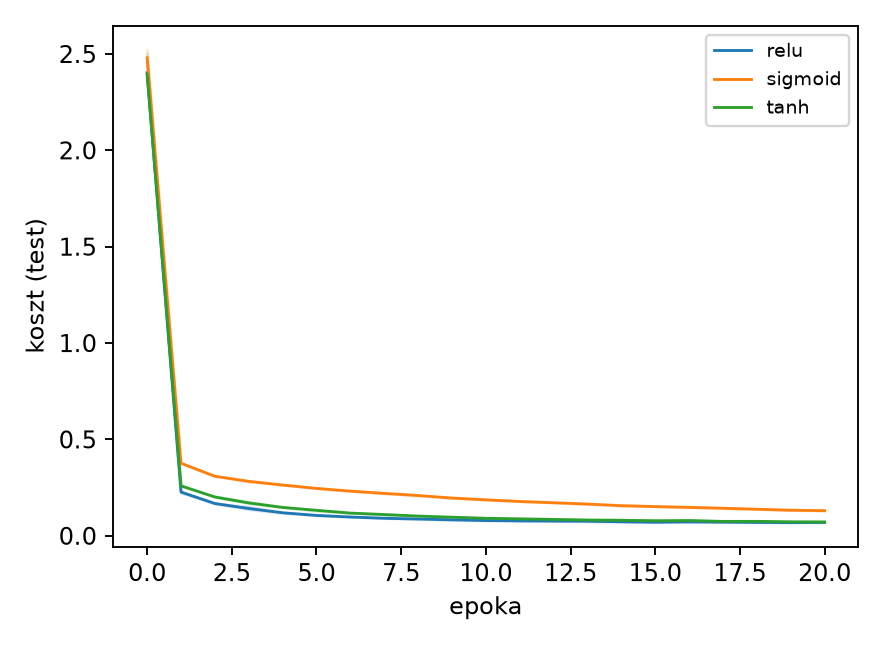
\includegraphics[width=0.7\linewidth]{figures/mnist/activation_curve_test_cost.png}
  \caption{MNIST: przebieg koszt (test) w trakcie uczenia dla różnych funkcji aktywacji (współczynnik uczenia 0.1).}
  \label{fig:mnist:activation_curve_test_cost}
\end{figure}

\begin{figure}[htbp]
  \centering
  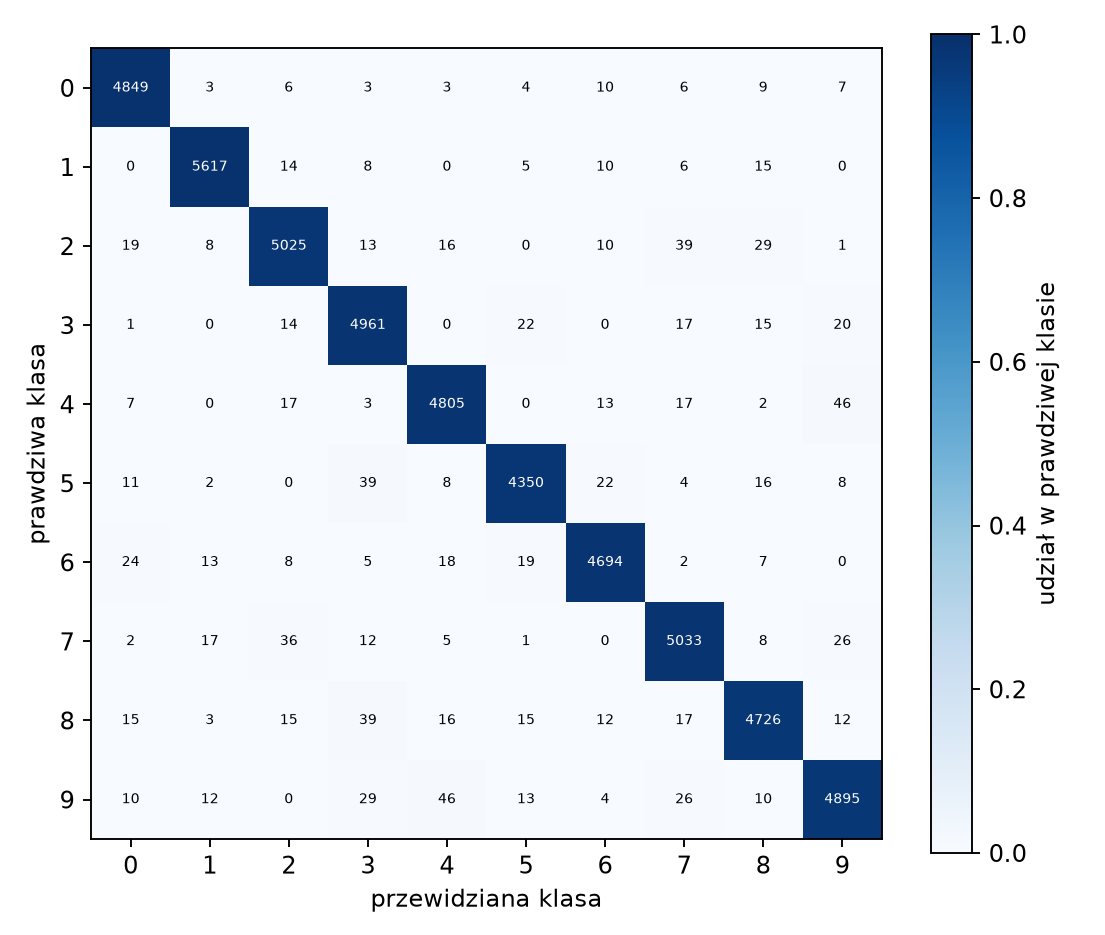
\includegraphics[width=0.7\linewidth]{figures/mnist/confusion_relu_128.png}
  \caption{MNIST: macierz pomyłek na zbiorze testowym, aktywacja relu, architektura 128, suma po 5 ziarnach (accuracy 0.979).}
  \label{fig:mnist:confusion_relu_128}
\end{figure}

\begin{figure}[htbp]
  \centering
  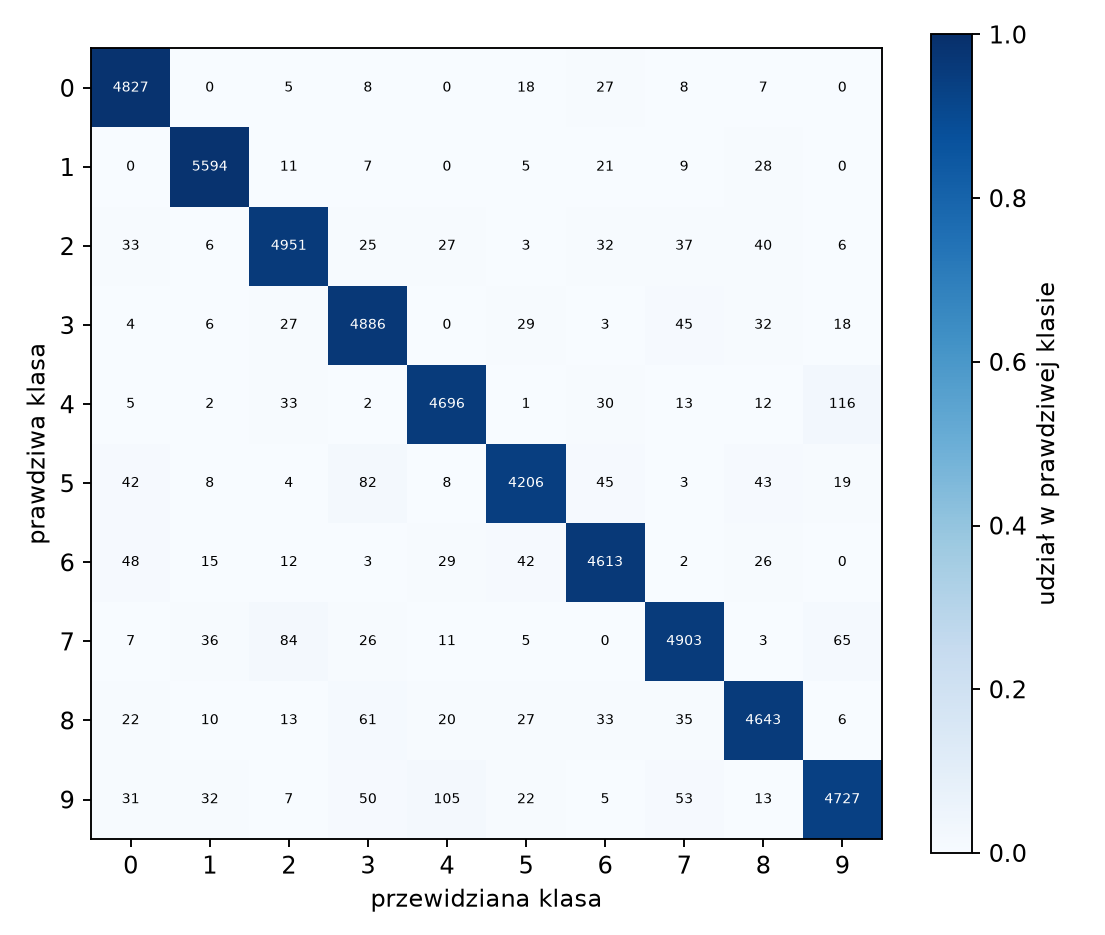
\includegraphics[width=0.7\linewidth]{figures/mnist/confusion_sigmoid_128.png}
  \caption{MNIST: macierz pomyłek na zbiorze testowym, aktywacja sigmoid, architektura 128, suma po 5 ziarnach (accuracy 0.961).}
  \label{fig:mnist:confusion_sigmoid_128}
\end{figure}

\begin{figure}[htbp]
  \centering
  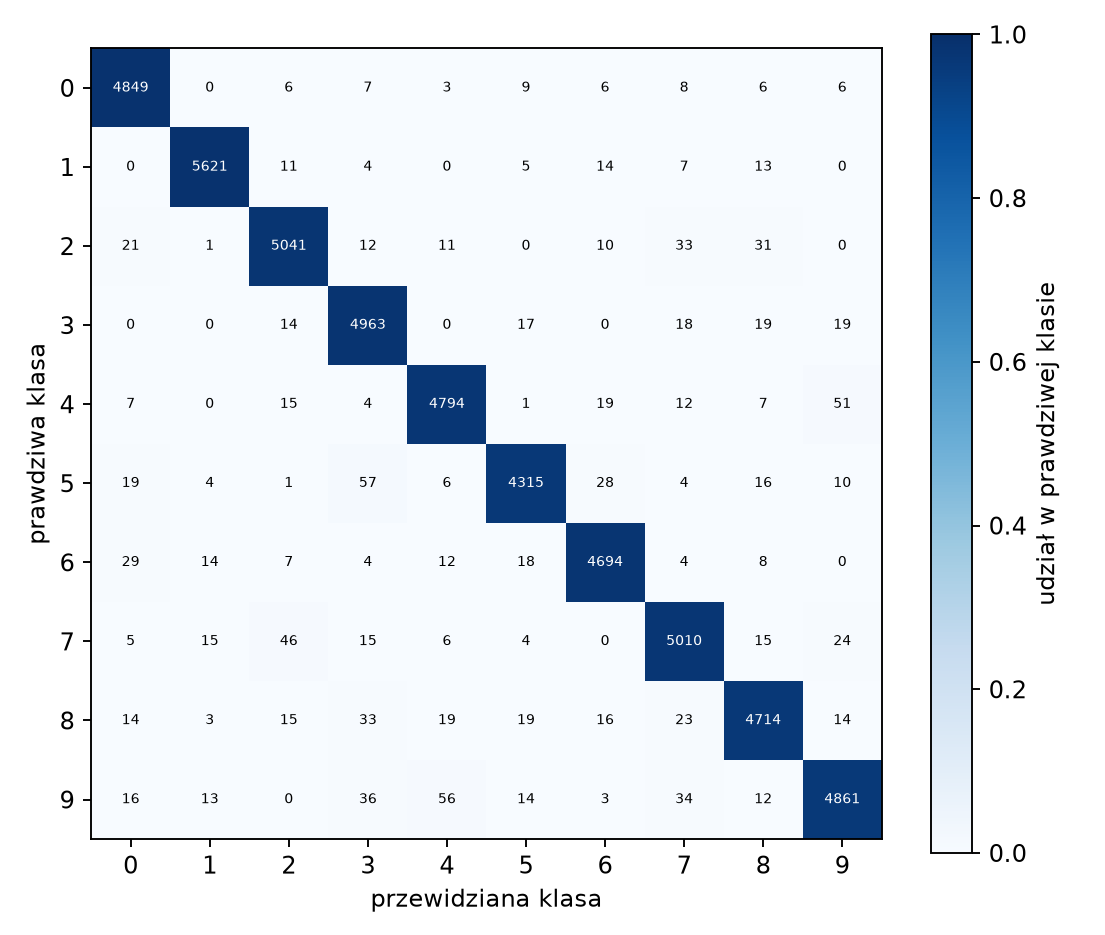
\includegraphics[width=0.7\linewidth]{figures/mnist/confusion_tanh_128.png}
  \caption{MNIST: macierz pomyłek na zbiorze testowym, aktywacja tanh, architektura 128, suma po 5 ziarnach (accuracy 0.977).}
  \label{fig:mnist:confusion_tanh_128}
\end{figure}

\begin{figure}[htbp]
  \centering
  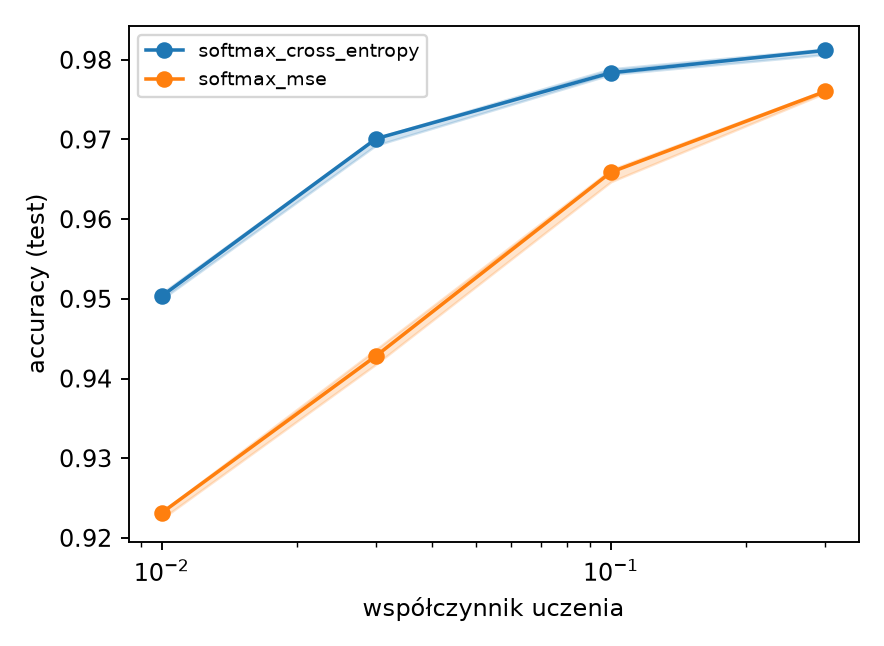
\includegraphics[width=0.7\linewidth]{figures/mnist/loss_lr_test_accuracy.png}
  \caption{MNIST: accuracy (test) dla różnych funkcji kosztu w zależności od współczynnika uczenia (mediana i kwartyle; liczba przy krzyżyku nad wykresem to liczba rozbieżnych ziaren).}
  \label{fig:mnist:loss_lr_test_accuracy}
\end{figure}

\begin{figure}[htbp]
  \centering
  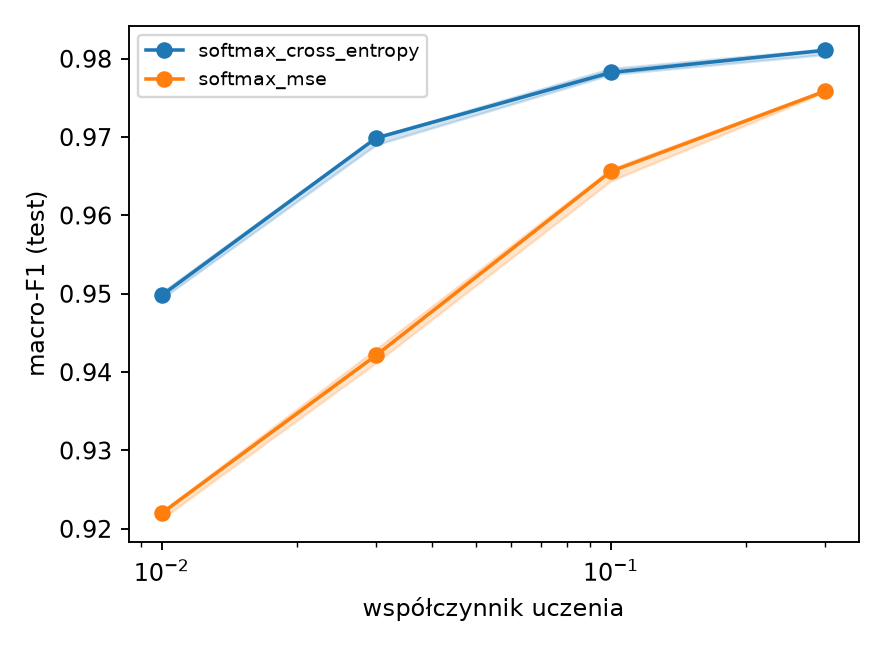
\includegraphics[width=0.7\linewidth]{figures/mnist/loss_lr_test_macro_f1.png}
  \caption{MNIST: macro-F1 (test) dla różnych funkcji kosztu w zależności od współczynnika uczenia (mediana i kwartyle; liczba przy krzyżyku nad wykresem to liczba rozbieżnych ziaren).}
  \label{fig:mnist:loss_lr_test_macro_f1}
\end{figure}

\begin{figure}[htbp]
  \centering
  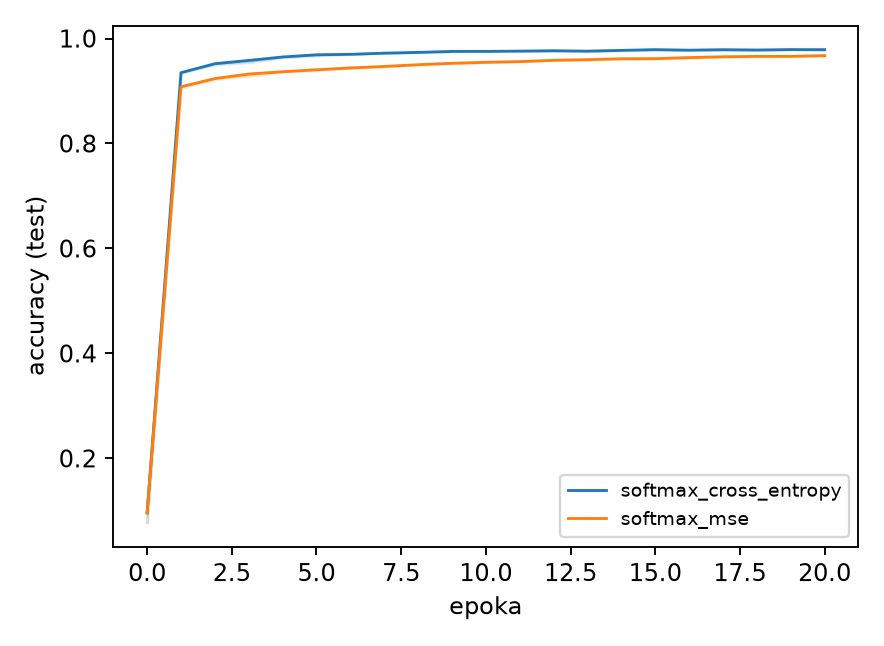
\includegraphics[width=0.7\linewidth]{figures/mnist/loss_curve_test_accuracy.png}
  \caption{MNIST: przebieg accuracy (test) w trakcie uczenia dla różnych funkcji kosztu (współczynnik uczenia 0.1).}
  \label{fig:mnist:loss_curve_test_accuracy}
\end{figure}

\begin{figure}[htbp]
  \centering
  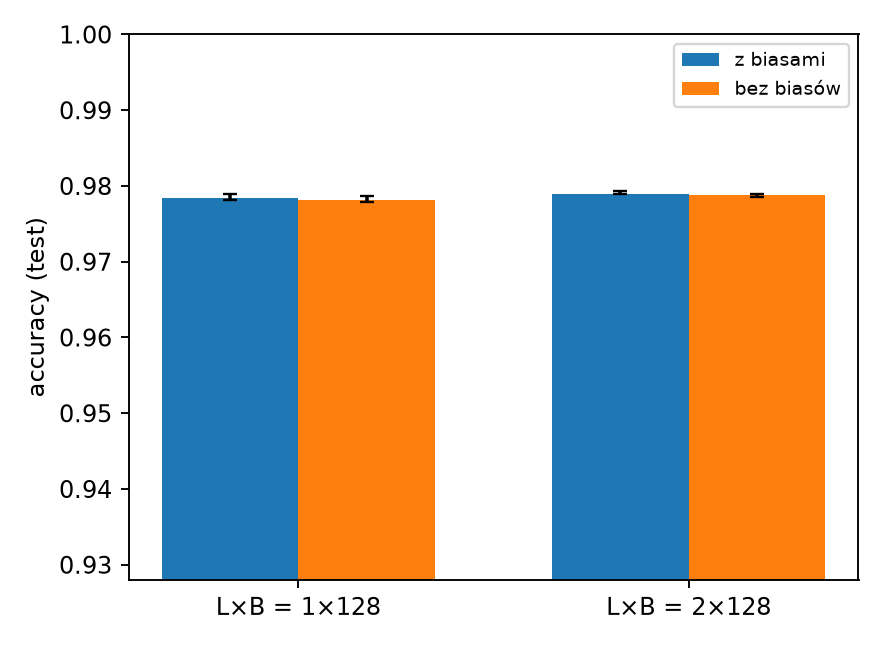
\includegraphics[width=0.7\linewidth]{figures/mnist/bias.png}
  \caption{MNIST: accuracy (test) sieci z biasami i bez biasów.}
  \label{fig:mnist:bias}
\end{figure}
 or copy single blocks.

\begin{figure}[htbp]
  \centering
  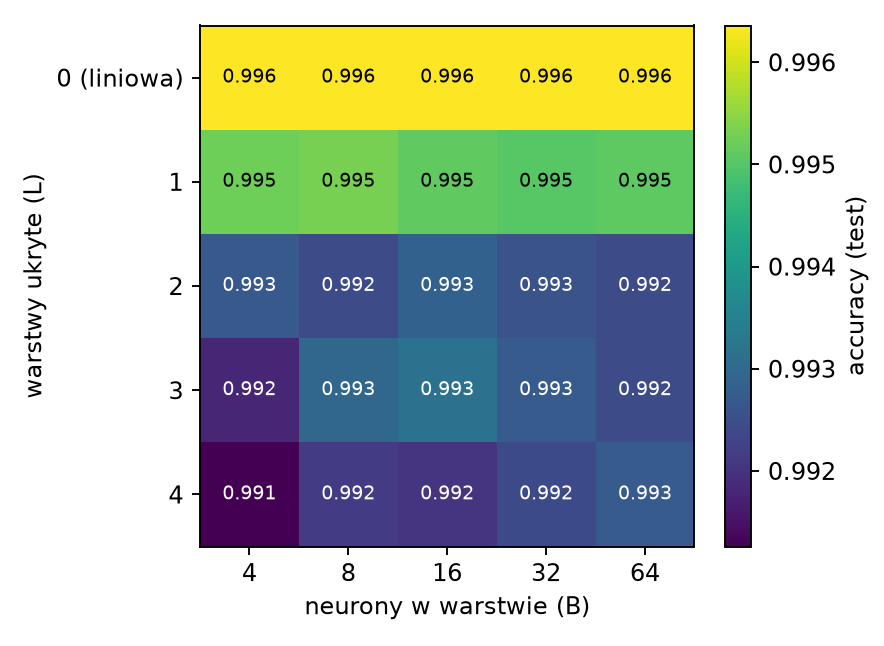
\includegraphics[width=0.7\linewidth]{figures/simple/arch_heatmap_test_accuracy.png}
  \caption{simple: accuracy (test) (mediana) w zależności od liczby warstw ukrytych $L$ i neuronów w warstwie $B$.}
  \label{fig:simple:arch_heatmap_test_accuracy}
\end{figure}

\begin{figure}[htbp]
  \centering
  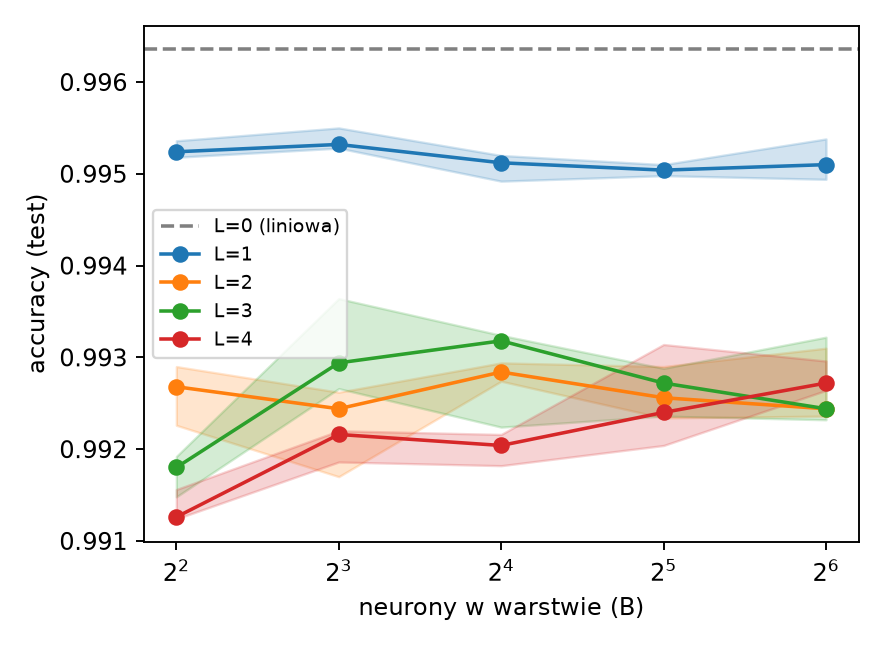
\includegraphics[width=0.7\linewidth]{figures/simple/arch_lines_test_accuracy.png}
  \caption{simple: accuracy (test) w zależności od $B$ dla każdej liczby warstw $L$ (mediana i kwartyle po ziarnach).}
  \label{fig:simple:arch_lines_test_accuracy}
\end{figure}

\begin{figure}[htbp]
  \centering
  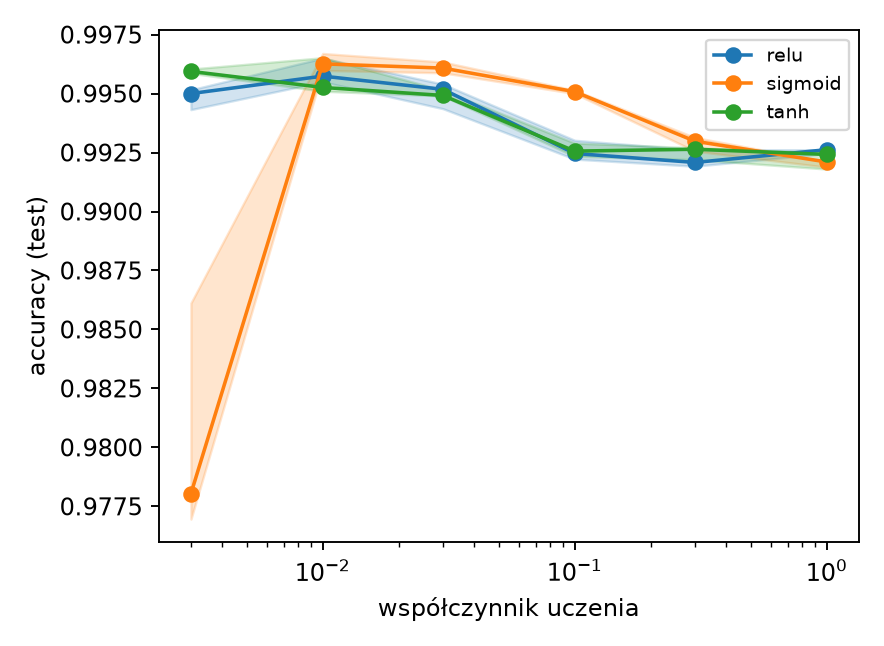
\includegraphics[width=0.7\linewidth]{figures/simple/activation_lr_test_accuracy.png}
  \caption{simple: accuracy (test) dla różnych funkcji aktywacji w zależności od współczynnika uczenia (mediana i kwartyle; liczba przy krzyżyku nad wykresem to liczba rozbieżnych ziaren).}
  \label{fig:simple:activation_lr_test_accuracy}
\end{figure}

\begin{figure}[htbp]
  \centering
  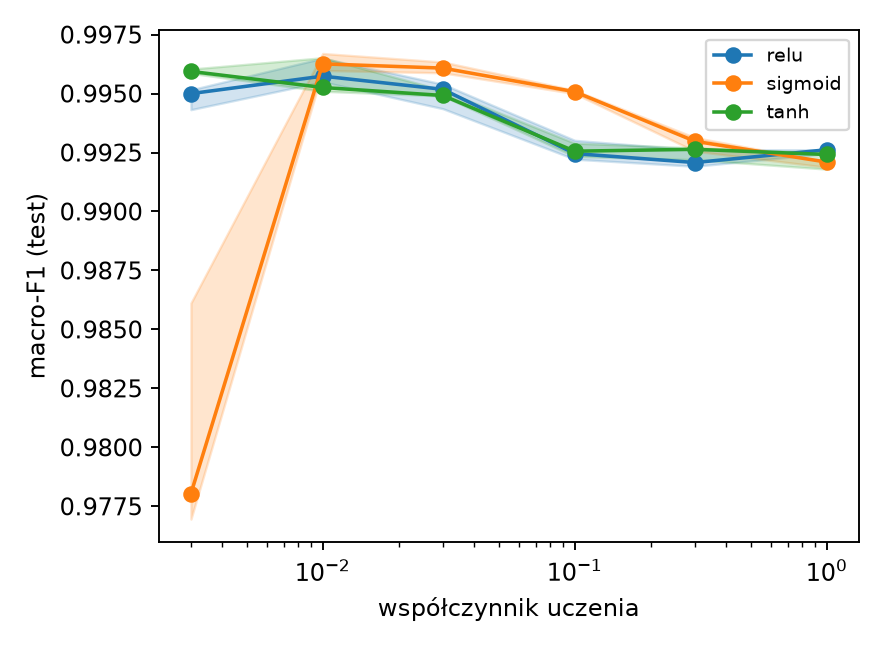
\includegraphics[width=0.7\linewidth]{figures/simple/activation_lr_test_macro_f1.png}
  \caption{simple: macro-F1 (test) dla różnych funkcji aktywacji w zależności od współczynnika uczenia (mediana i kwartyle; liczba przy krzyżyku nad wykresem to liczba rozbieżnych ziaren).}
  \label{fig:simple:activation_lr_test_macro_f1}
\end{figure}

\begin{figure}[htbp]
  \centering
  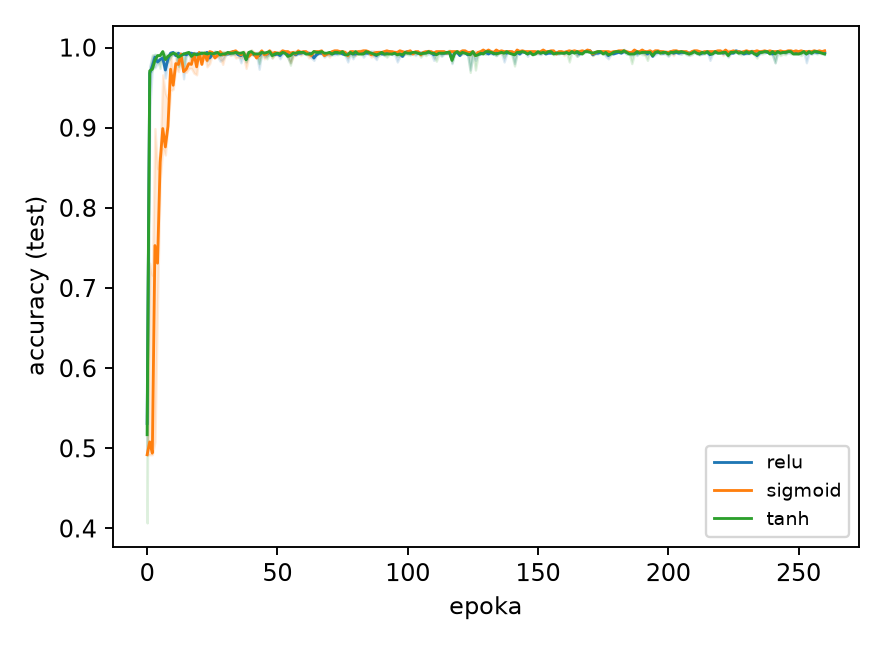
\includegraphics[width=0.7\linewidth]{figures/simple/activation_curve_test_accuracy.png}
  \caption{simple: przebieg accuracy (test) w trakcie uczenia dla różnych funkcji aktywacji (współczynnik uczenia 0.1).}
  \label{fig:simple:activation_curve_test_accuracy}
\end{figure}

\begin{figure}[htbp]
  \centering
  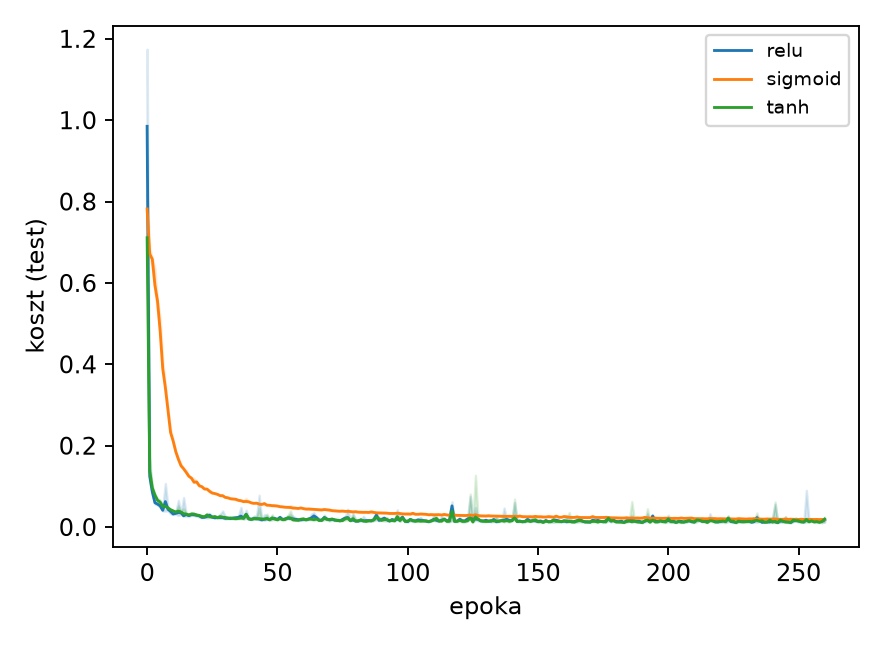
\includegraphics[width=0.7\linewidth]{figures/simple/activation_curve_test_cost.png}
  \caption{simple: przebieg koszt (test) w trakcie uczenia dla różnych funkcji aktywacji (współczynnik uczenia 0.1).}
  \label{fig:simple:activation_curve_test_cost}
\end{figure}

\begin{figure}[htbp]
  \centering
  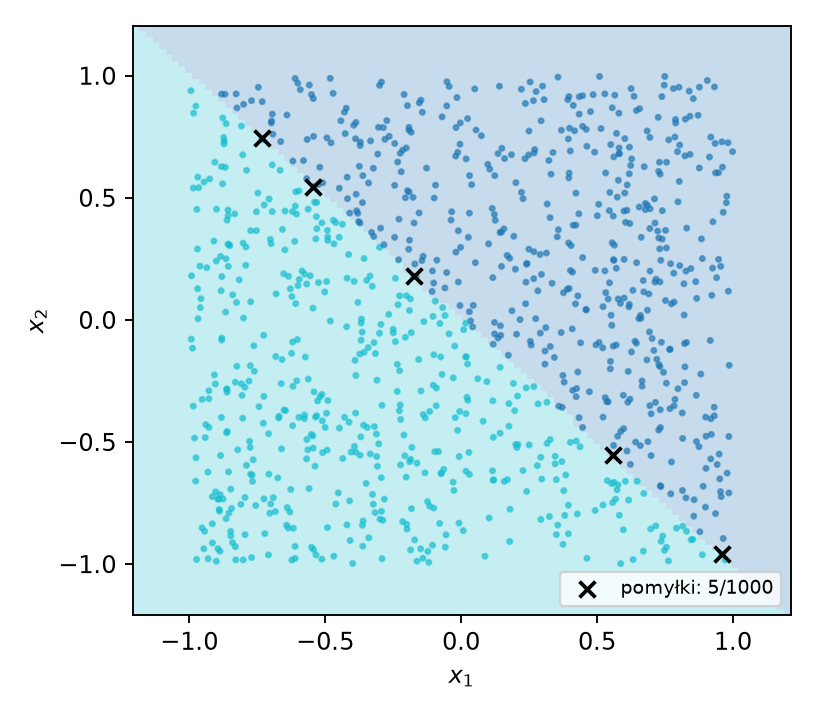
\includegraphics[width=0.7\linewidth]{figures/simple/predictions_relu.png}
  \caption{simple: obszary decyzyjne sieci z aktywacją relu (ziarno 0). Punkty testowe w kolorze prawdziwej klasy, × oznacza pomyłkę (accuracy 0.995).}
  \label{fig:simple:predictions_relu}
\end{figure}

\begin{figure}[htbp]
  \centering
  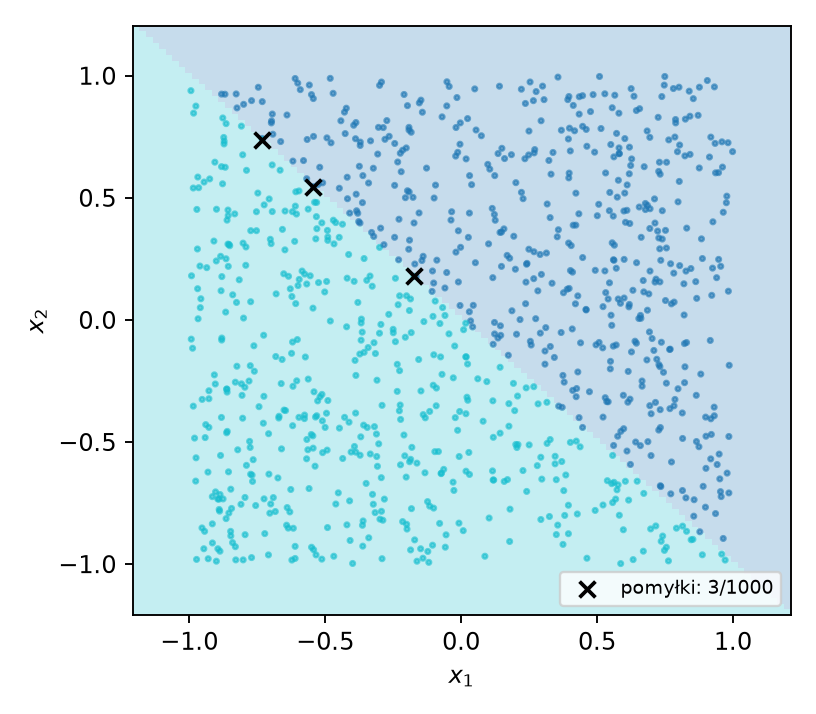
\includegraphics[width=0.7\linewidth]{figures/simple/predictions_sigmoid.png}
  \caption{simple: obszary decyzyjne sieci z aktywacją sigmoid (ziarno 0). Punkty testowe w kolorze prawdziwej klasy, × oznacza pomyłkę (accuracy 0.997).}
  \label{fig:simple:predictions_sigmoid}
\end{figure}

\begin{figure}[htbp]
  \centering
  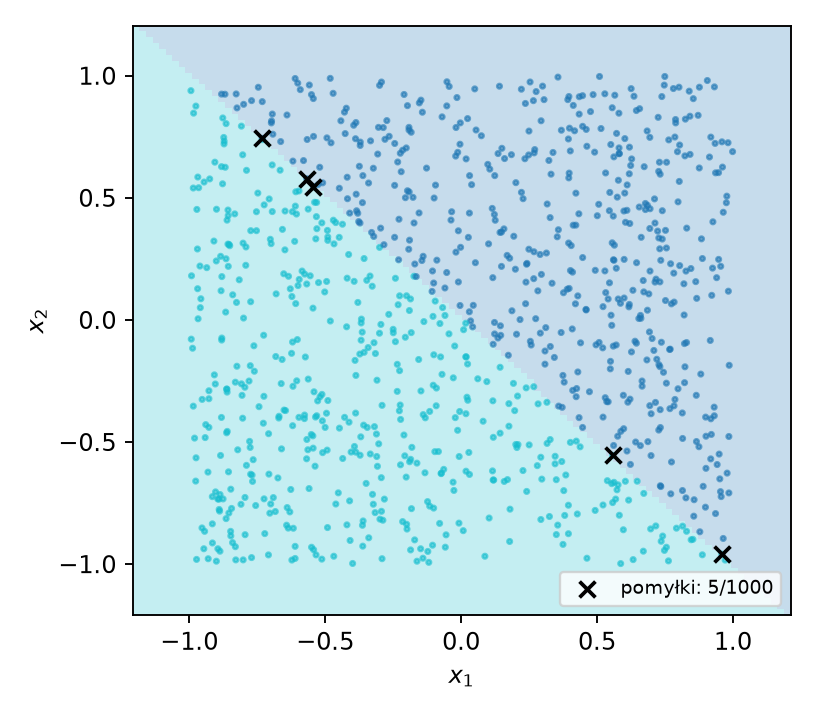
\includegraphics[width=0.7\linewidth]{figures/simple/predictions_tanh.png}
  \caption{simple: obszary decyzyjne sieci z aktywacją tanh (ziarno 0). Punkty testowe w kolorze prawdziwej klasy, × oznacza pomyłkę (accuracy 0.995).}
  \label{fig:simple:predictions_tanh}
\end{figure}

\begin{figure}[htbp]
  \centering
  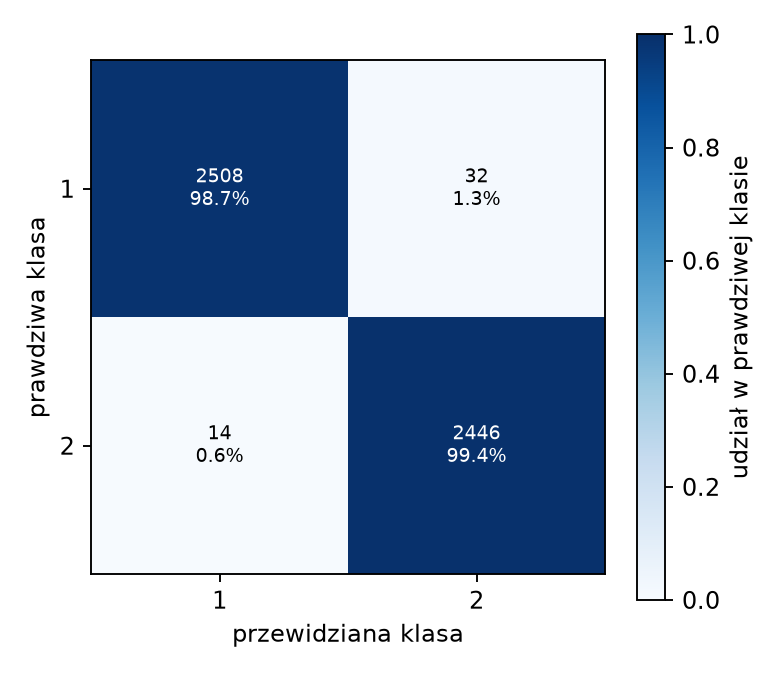
\includegraphics[width=0.7\linewidth]{figures/simple/confusion_relu_32x32.png}
  \caption{simple: macierz pomyłek na zbiorze testowym, aktywacja relu, architektura 32x32, suma po 5 ziarnach (accuracy 0.991).}
  \label{fig:simple:confusion_relu_32x32}
\end{figure}

\begin{figure}[htbp]
  \centering
  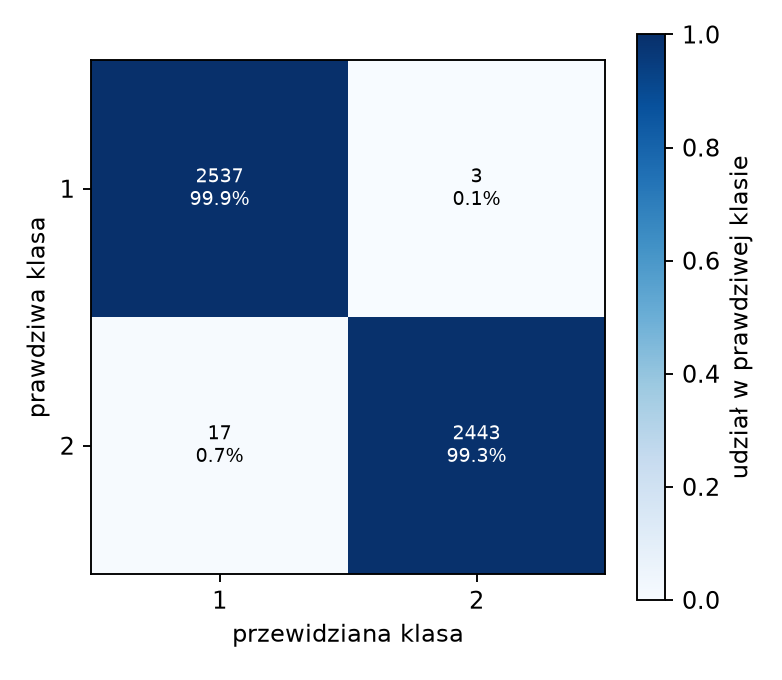
\includegraphics[width=0.7\linewidth]{figures/simple/confusion_sigmoid_32x32.png}
  \caption{simple: macierz pomyłek na zbiorze testowym, aktywacja sigmoid, architektura 32x32, suma po 5 ziarnach (accuracy 0.996).}
  \label{fig:simple:confusion_sigmoid_32x32}
\end{figure}

\begin{figure}[htbp]
  \centering
  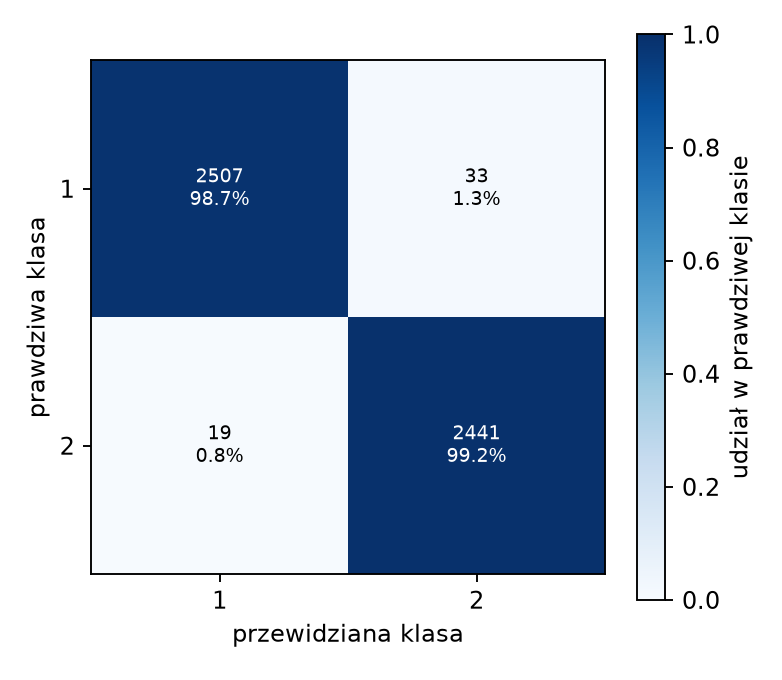
\includegraphics[width=0.7\linewidth]{figures/simple/confusion_tanh_32x32.png}
  \caption{simple: macierz pomyłek na zbiorze testowym, aktywacja tanh, architektura 32x32, suma po 5 ziarnach (accuracy 0.990).}
  \label{fig:simple:confusion_tanh_32x32}
\end{figure}

\begin{figure}[htbp]
  \centering
  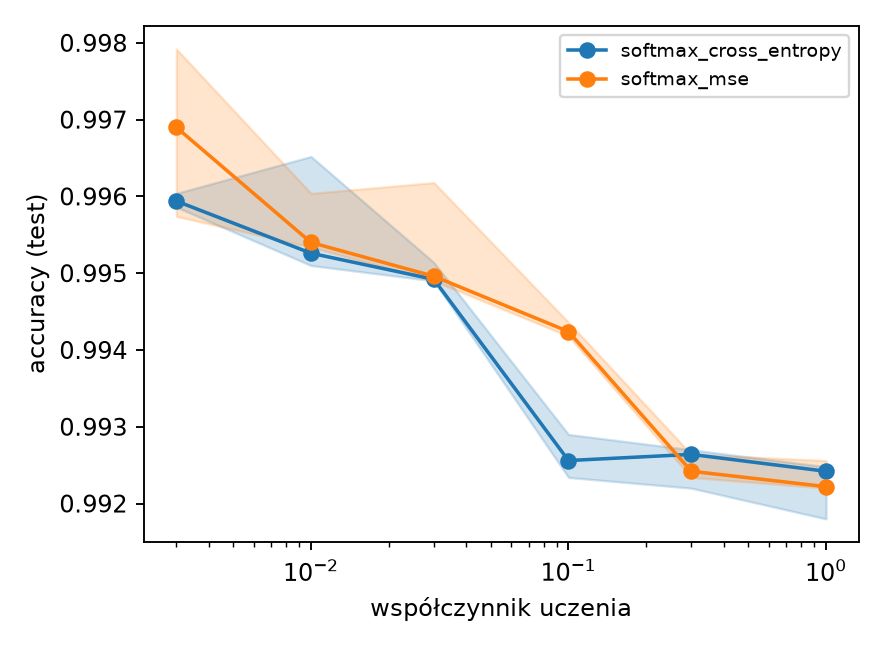
\includegraphics[width=0.7\linewidth]{figures/simple/loss_lr_test_accuracy.png}
  \caption{simple: accuracy (test) dla różnych funkcji kosztu w zależności od współczynnika uczenia (mediana i kwartyle; liczba przy krzyżyku nad wykresem to liczba rozbieżnych ziaren).}
  \label{fig:simple:loss_lr_test_accuracy}
\end{figure}

\begin{figure}[htbp]
  \centering
  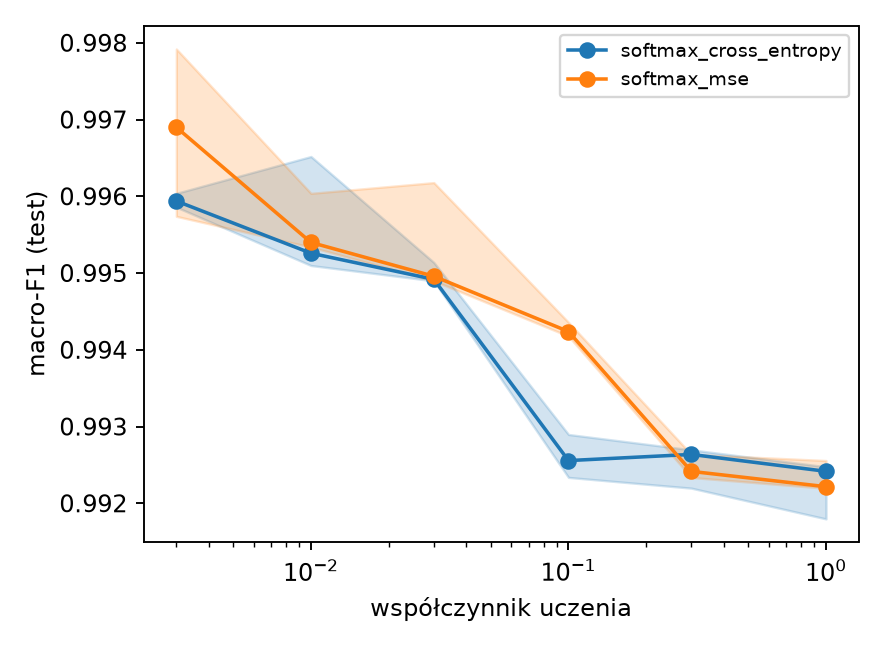
\includegraphics[width=0.7\linewidth]{figures/simple/loss_lr_test_macro_f1.png}
  \caption{simple: macro-F1 (test) dla różnych funkcji kosztu w zależności od współczynnika uczenia (mediana i kwartyle; liczba przy krzyżyku nad wykresem to liczba rozbieżnych ziaren).}
  \label{fig:simple:loss_lr_test_macro_f1}
\end{figure}

\begin{figure}[htbp]
  \centering
  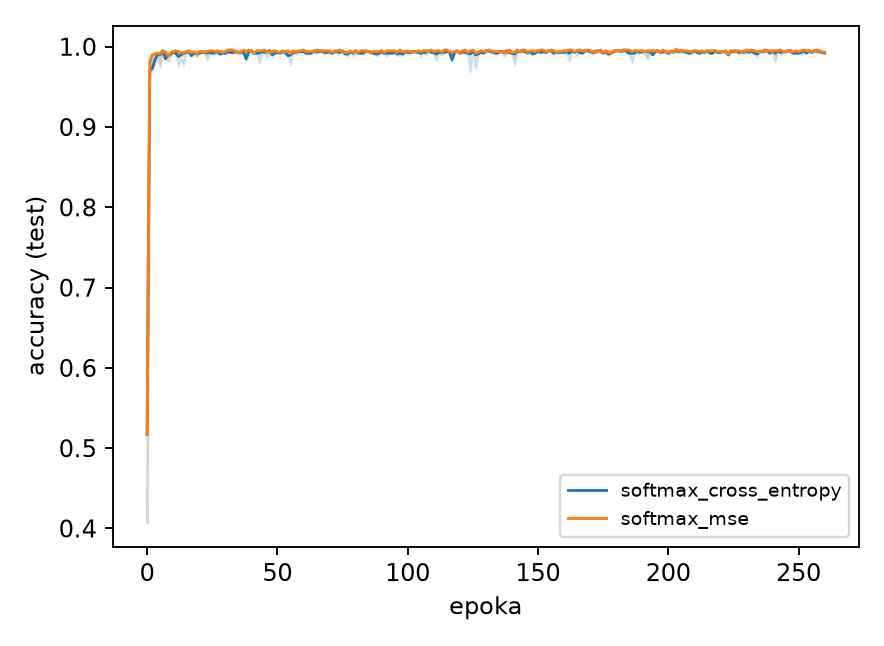
\includegraphics[width=0.7\linewidth]{figures/simple/loss_curve_test_accuracy.png}
  \caption{simple: przebieg accuracy (test) w trakcie uczenia dla różnych funkcji kosztu (współczynnik uczenia 0.1).}
  \label{fig:simple:loss_curve_test_accuracy}
\end{figure}

\begin{figure}[htbp]
  \centering
  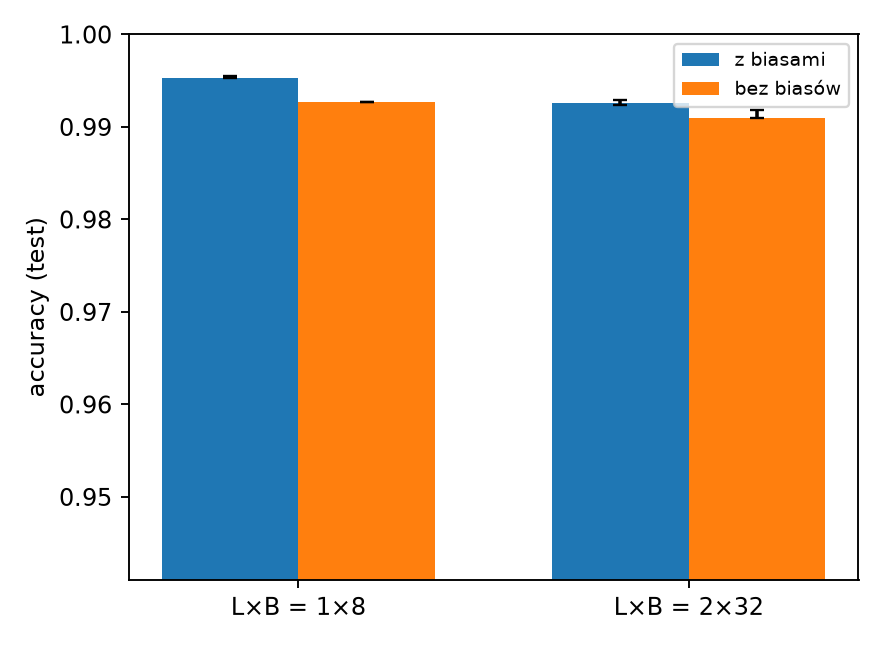
\includegraphics[width=0.7\linewidth]{figures/simple/bias.png}
  \caption{simple: accuracy (test) sieci z biasami i bez biasów.}
  \label{fig:simple:bias}
\end{figure}

\begin{figure}[htbp]
  \centering
  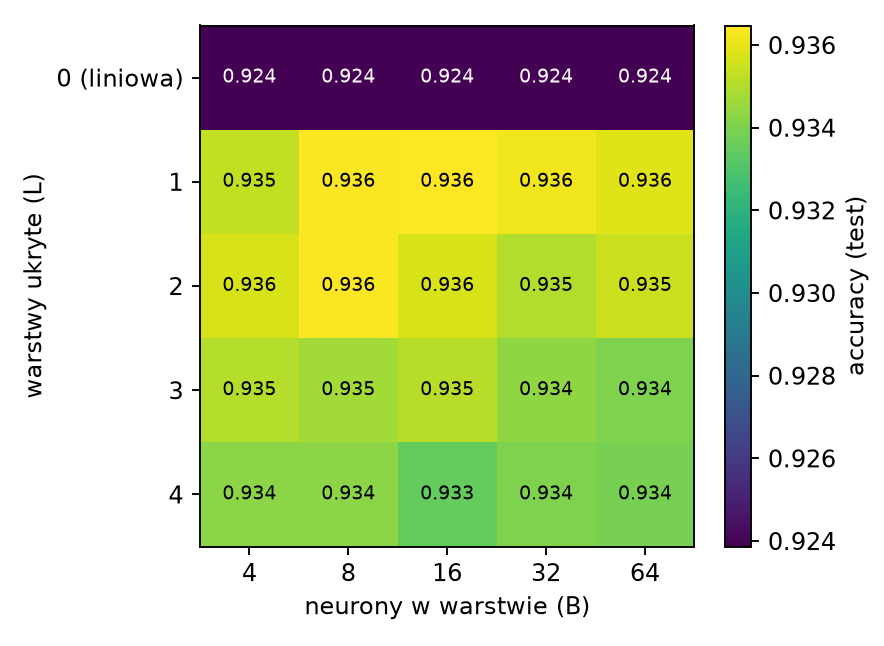
\includegraphics[width=0.7\linewidth]{figures/three_gauss/arch_heatmap_test_accuracy.png}
  \caption{three\_gauss: accuracy (test) (mediana) w zależności od liczby warstw ukrytych $L$ i neuronów w warstwie $B$.}
  \label{fig:three_gauss:arch_heatmap_test_accuracy}
\end{figure}

\begin{figure}[htbp]
  \centering
  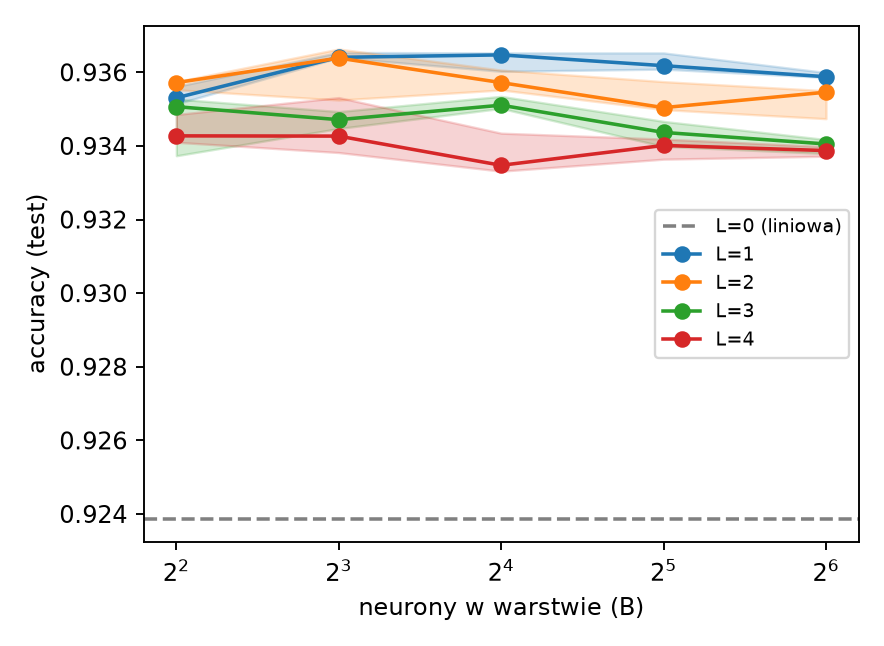
\includegraphics[width=0.7\linewidth]{figures/three_gauss/arch_lines_test_accuracy.png}
  \caption{three\_gauss: accuracy (test) w zależności od $B$ dla każdej liczby warstw $L$ (mediana i kwartyle po ziarnach).}
  \label{fig:three_gauss:arch_lines_test_accuracy}
\end{figure}

\begin{figure}[htbp]
  \centering
  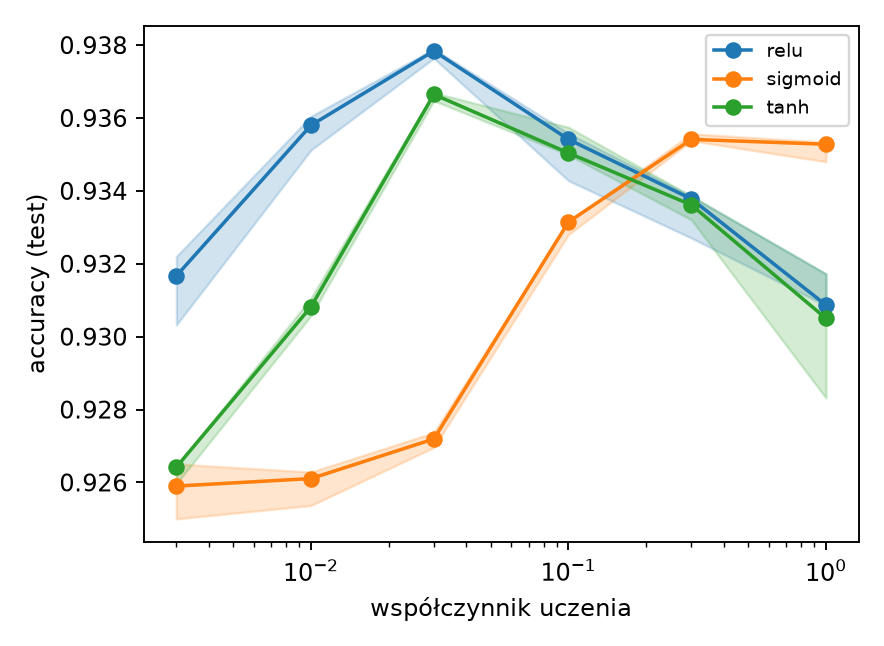
\includegraphics[width=0.7\linewidth]{figures/three_gauss/activation_lr_test_accuracy.png}
  \caption{three\_gauss: accuracy (test) dla różnych funkcji aktywacji w zależności od współczynnika uczenia (mediana i kwartyle; liczba przy krzyżyku nad wykresem to liczba rozbieżnych ziaren).}
  \label{fig:three_gauss:activation_lr_test_accuracy}
\end{figure}

\begin{figure}[htbp]
  \centering
  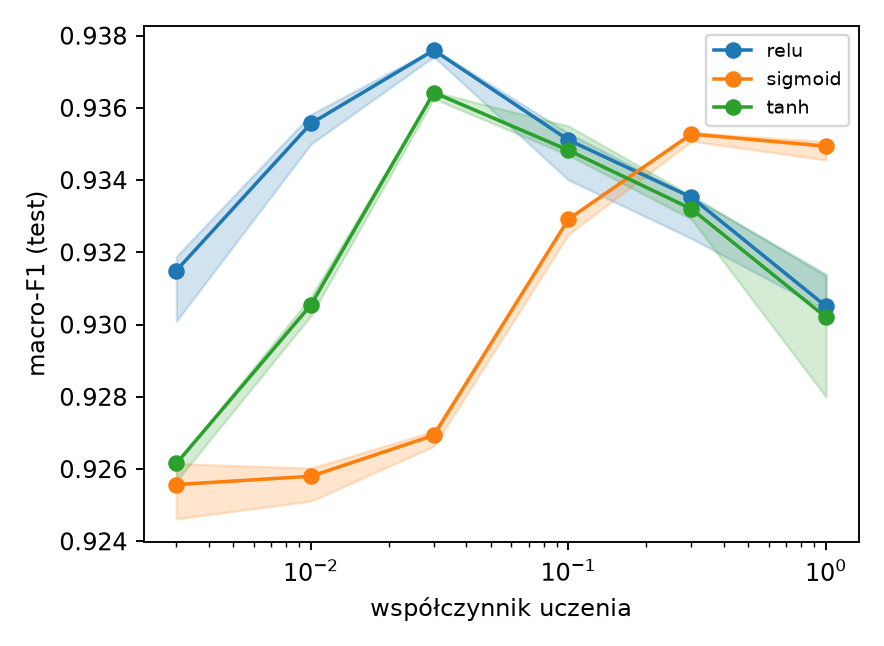
\includegraphics[width=0.7\linewidth]{figures/three_gauss/activation_lr_test_macro_f1.png}
  \caption{three\_gauss: macro-F1 (test) dla różnych funkcji aktywacji w zależności od współczynnika uczenia (mediana i kwartyle; liczba przy krzyżyku nad wykresem to liczba rozbieżnych ziaren).}
  \label{fig:three_gauss:activation_lr_test_macro_f1}
\end{figure}

\begin{figure}[htbp]
  \centering
  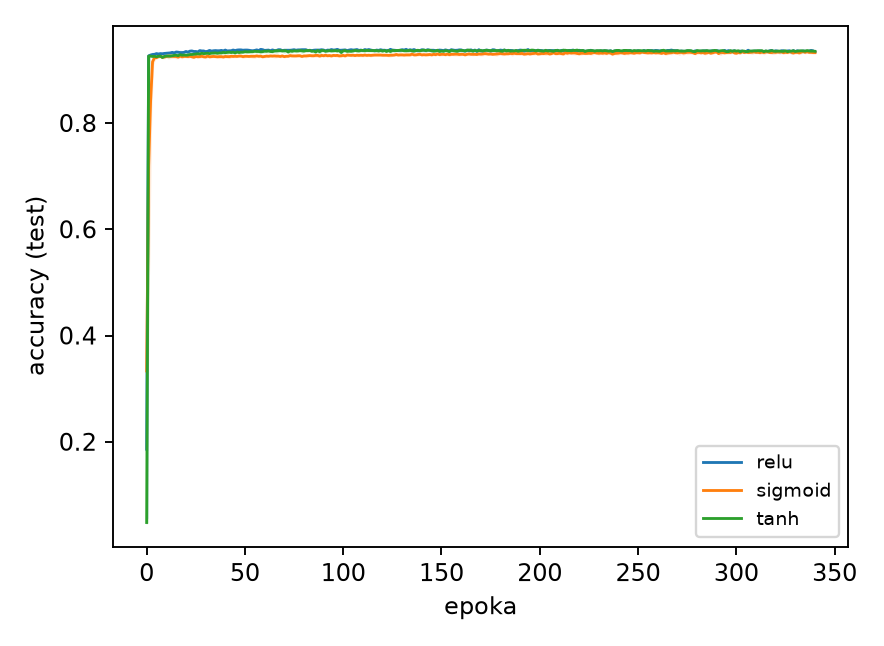
\includegraphics[width=0.7\linewidth]{figures/three_gauss/activation_curve_test_accuracy.png}
  \caption{three\_gauss: przebieg accuracy (test) w trakcie uczenia dla różnych funkcji aktywacji (współczynnik uczenia 0.1).}
  \label{fig:three_gauss:activation_curve_test_accuracy}
\end{figure}

\begin{figure}[htbp]
  \centering
  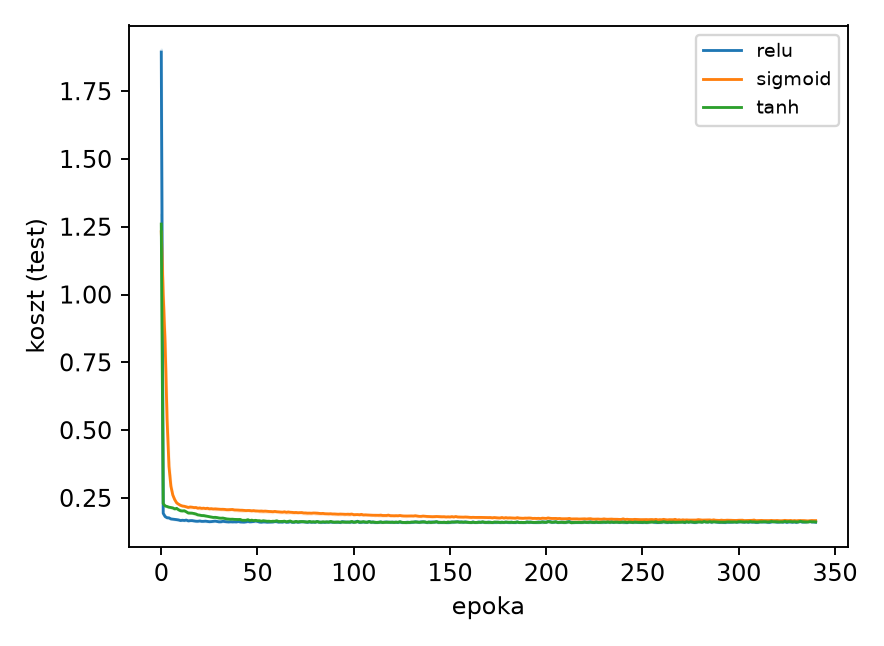
\includegraphics[width=0.7\linewidth]{figures/three_gauss/activation_curve_test_cost.png}
  \caption{three\_gauss: przebieg koszt (test) w trakcie uczenia dla różnych funkcji aktywacji (współczynnik uczenia 0.1).}
  \label{fig:three_gauss:activation_curve_test_cost}
\end{figure}

\begin{figure}[htbp]
  \centering
  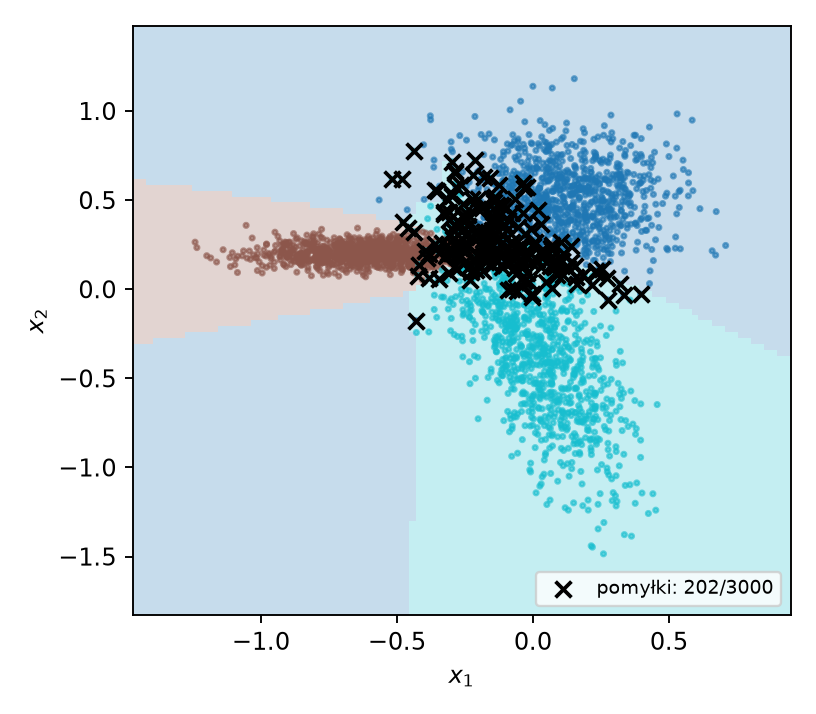
\includegraphics[width=0.7\linewidth]{figures/three_gauss/predictions_relu.png}
  \caption{three\_gauss: obszary decyzyjne sieci z aktywacją relu (ziarno 0). Punkty testowe w kolorze prawdziwej klasy, × oznacza pomyłkę (accuracy 0.933).}
  \label{fig:three_gauss:predictions_relu}
\end{figure}

\begin{figure}[htbp]
  \centering
  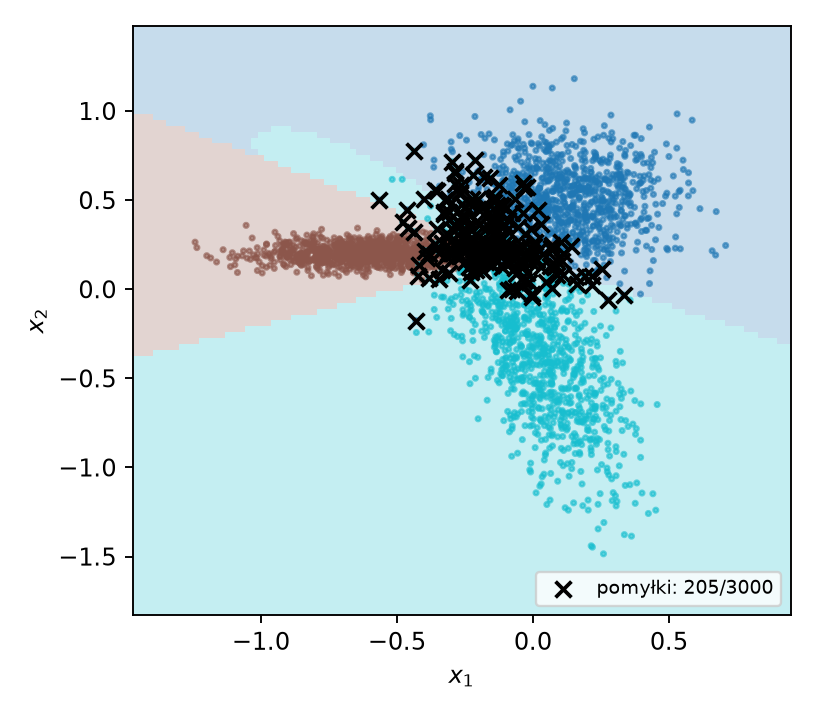
\includegraphics[width=0.7\linewidth]{figures/three_gauss/predictions_sigmoid.png}
  \caption{three\_gauss: obszary decyzyjne sieci z aktywacją sigmoid (ziarno 0). Punkty testowe w kolorze prawdziwej klasy, × oznacza pomyłkę (accuracy 0.932).}
  \label{fig:three_gauss:predictions_sigmoid}
\end{figure}

\begin{figure}[htbp]
  \centering
  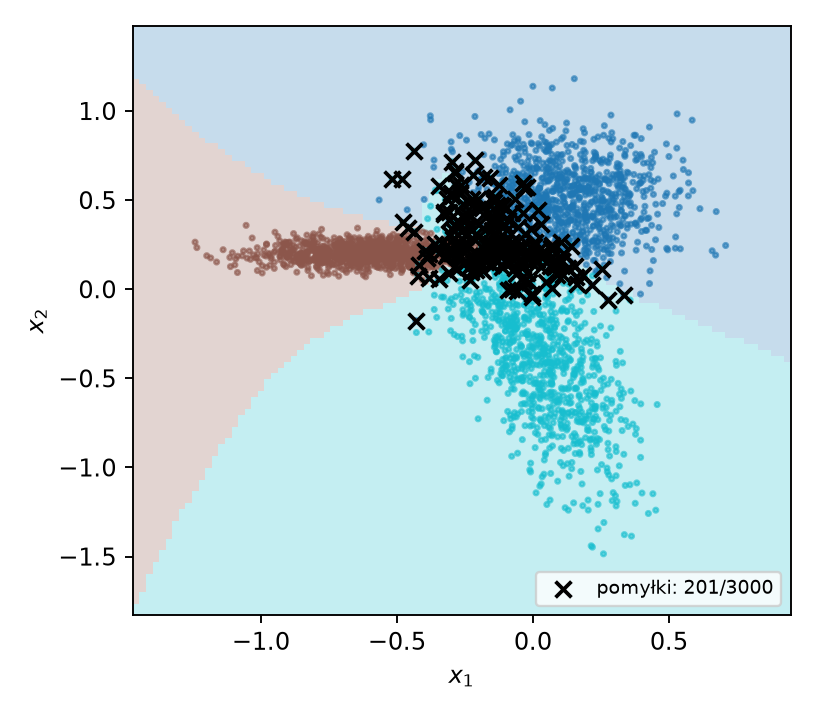
\includegraphics[width=0.7\linewidth]{figures/three_gauss/predictions_tanh.png}
  \caption{three\_gauss: obszary decyzyjne sieci z aktywacją tanh (ziarno 0). Punkty testowe w kolorze prawdziwej klasy, × oznacza pomyłkę (accuracy 0.933).}
  \label{fig:three_gauss:predictions_tanh}
\end{figure}

\begin{figure}[htbp]
  \centering
  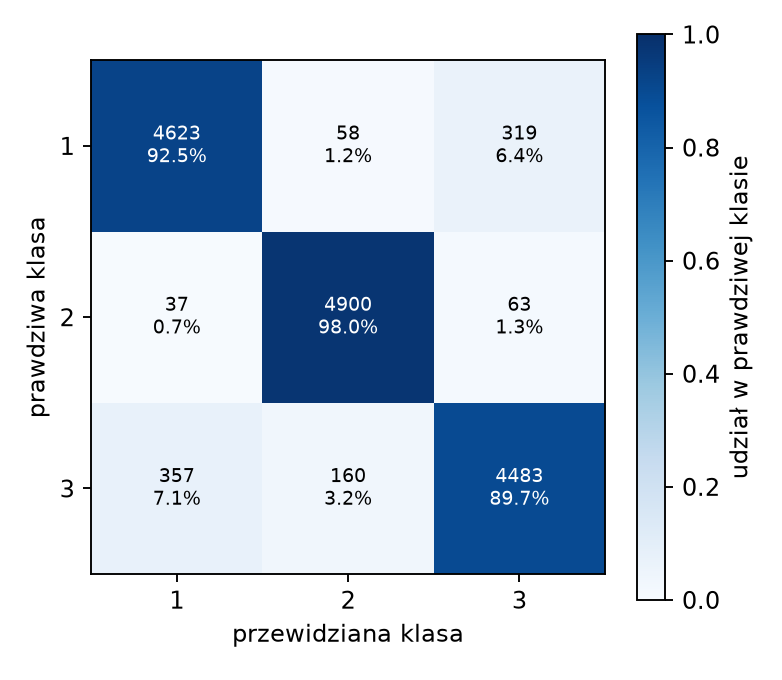
\includegraphics[width=0.7\linewidth]{figures/three_gauss/confusion_relu_32x32.png}
  \caption{three\_gauss: macierz pomyłek na zbiorze testowym, aktywacja relu, architektura 32x32, suma po 5 ziarnach (accuracy 0.934).}
  \label{fig:three_gauss:confusion_relu_32x32}
\end{figure}

\begin{figure}[htbp]
  \centering
  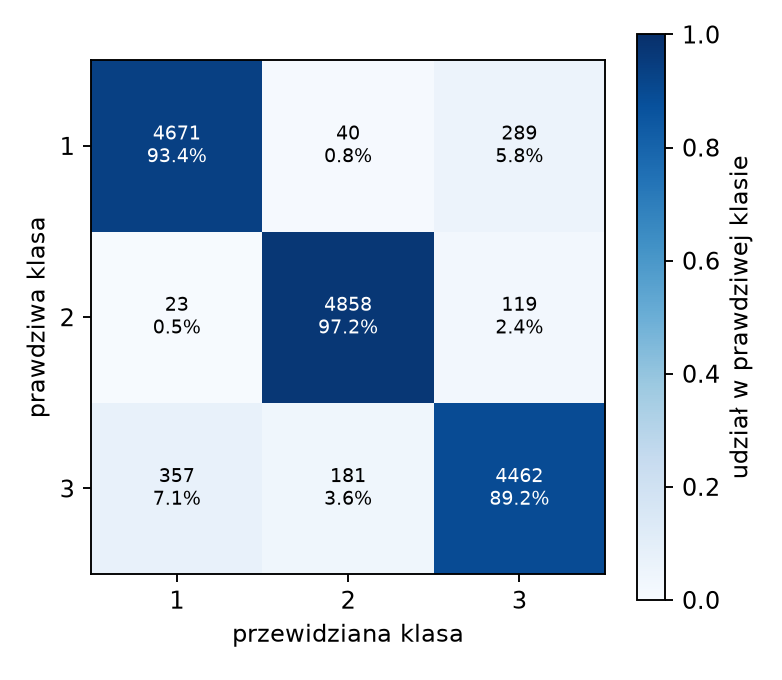
\includegraphics[width=0.7\linewidth]{figures/three_gauss/confusion_sigmoid_32x32.png}
  \caption{three\_gauss: macierz pomyłek na zbiorze testowym, aktywacja sigmoid, architektura 32x32, suma po 5 ziarnach (accuracy 0.933).}
  \label{fig:three_gauss:confusion_sigmoid_32x32}
\end{figure}

\begin{figure}[htbp]
  \centering
  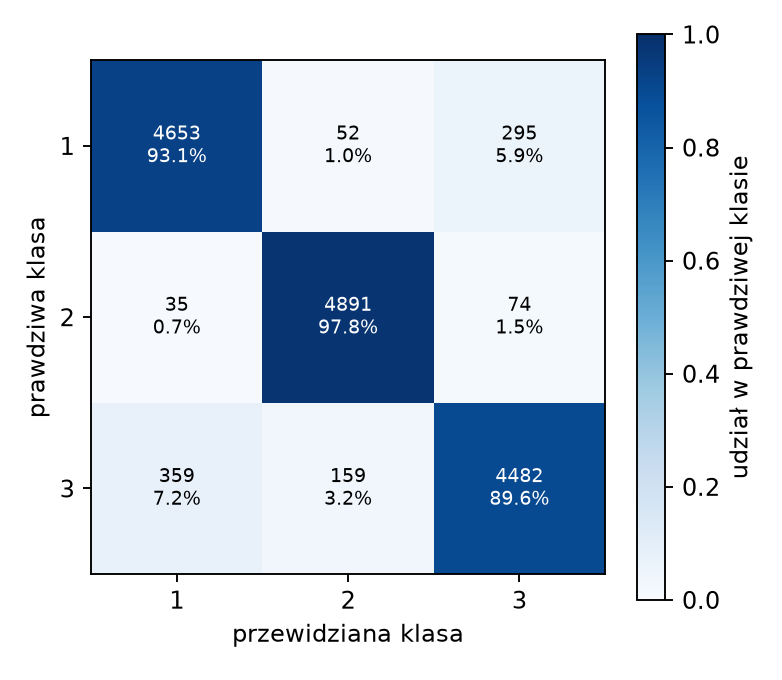
\includegraphics[width=0.7\linewidth]{figures/three_gauss/confusion_tanh_32x32.png}
  \caption{three\_gauss: macierz pomyłek na zbiorze testowym, aktywacja tanh, architektura 32x32, suma po 5 ziarnach (accuracy 0.935).}
  \label{fig:three_gauss:confusion_tanh_32x32}
\end{figure}

\begin{figure}[htbp]
  \centering
  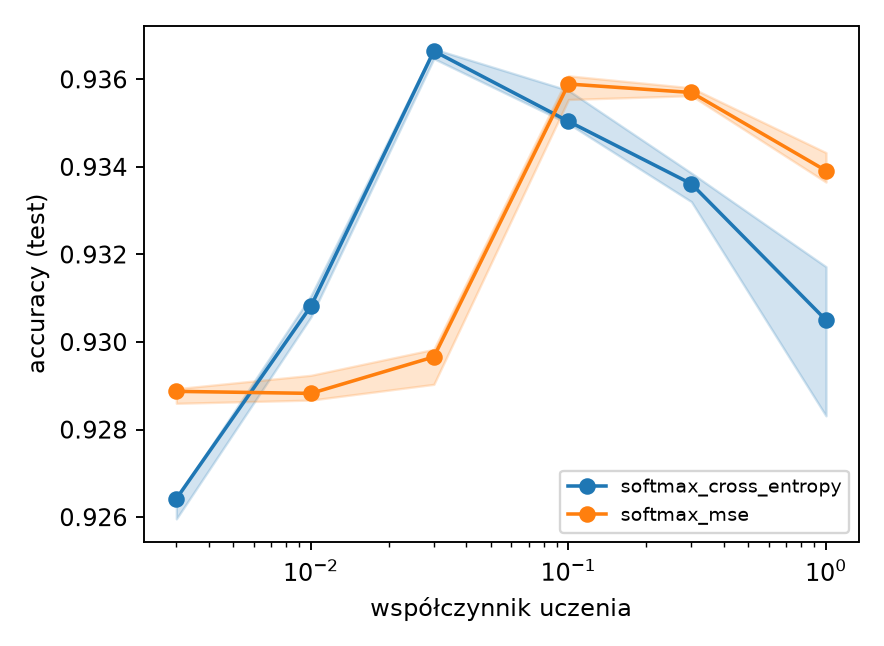
\includegraphics[width=0.7\linewidth]{figures/three_gauss/loss_lr_test_accuracy.png}
  \caption{three\_gauss: accuracy (test) dla różnych funkcji kosztu w zależności od współczynnika uczenia (mediana i kwartyle; liczba przy krzyżyku nad wykresem to liczba rozbieżnych ziaren).}
  \label{fig:three_gauss:loss_lr_test_accuracy}
\end{figure}

\begin{figure}[htbp]
  \centering
  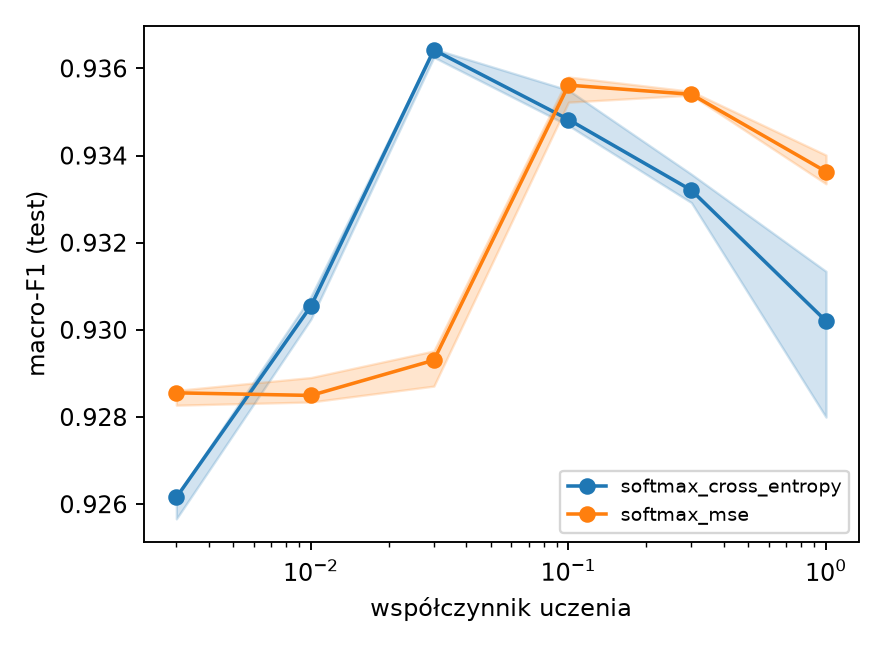
\includegraphics[width=0.7\linewidth]{figures/three_gauss/loss_lr_test_macro_f1.png}
  \caption{three\_gauss: macro-F1 (test) dla różnych funkcji kosztu w zależności od współczynnika uczenia (mediana i kwartyle; liczba przy krzyżyku nad wykresem to liczba rozbieżnych ziaren).}
  \label{fig:three_gauss:loss_lr_test_macro_f1}
\end{figure}

\begin{figure}[htbp]
  \centering
  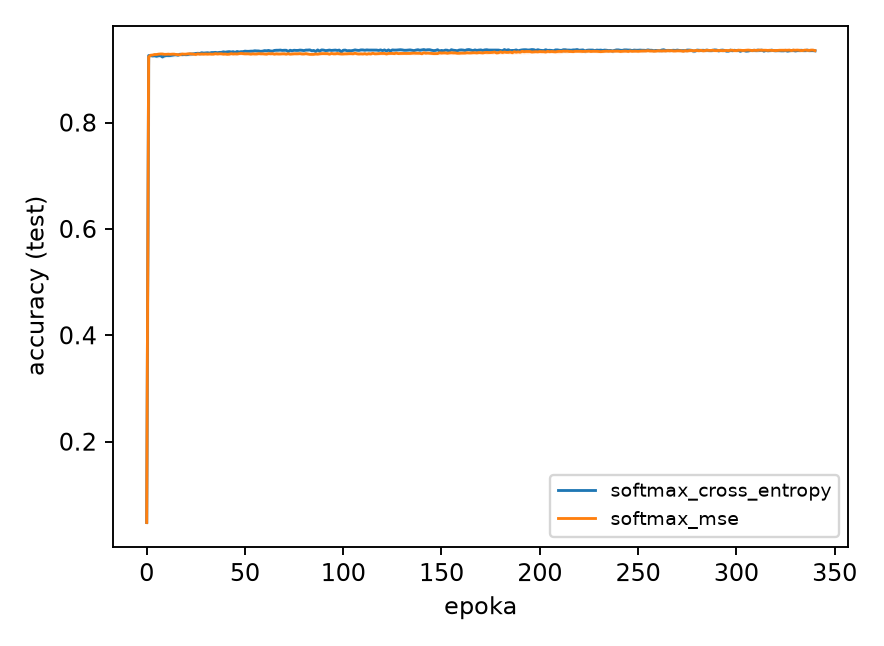
\includegraphics[width=0.7\linewidth]{figures/three_gauss/loss_curve_test_accuracy.png}
  \caption{three\_gauss: przebieg accuracy (test) w trakcie uczenia dla różnych funkcji kosztu (współczynnik uczenia 0.1).}
  \label{fig:three_gauss:loss_curve_test_accuracy}
\end{figure}

\begin{figure}[htbp]
  \centering
  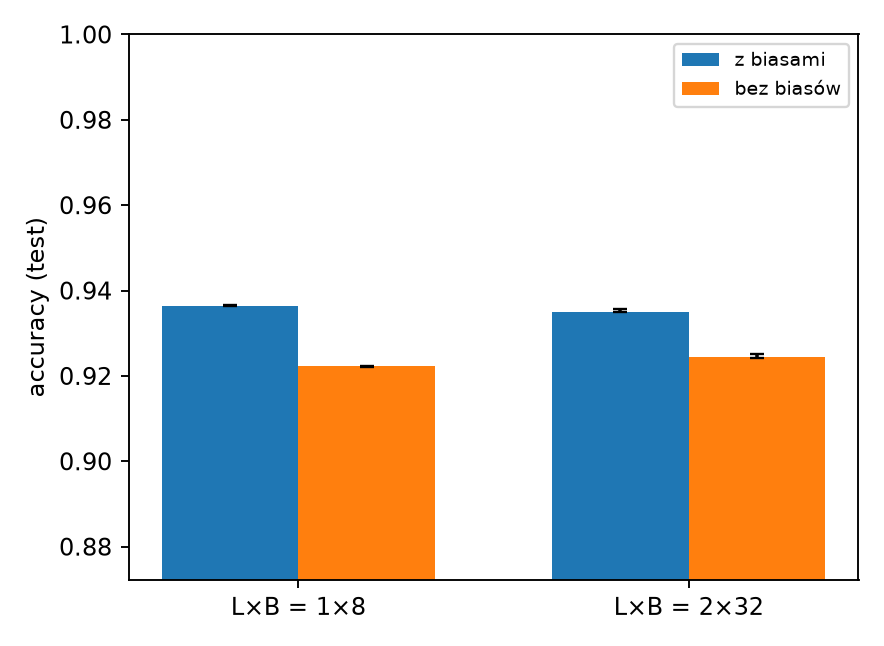
\includegraphics[width=0.7\linewidth]{figures/three_gauss/bias.png}
  \caption{three\_gauss: accuracy (test) sieci z biasami i bez biasów.}
  \label{fig:three_gauss:bias}
\end{figure}

\begin{figure}[htbp]
  \centering
  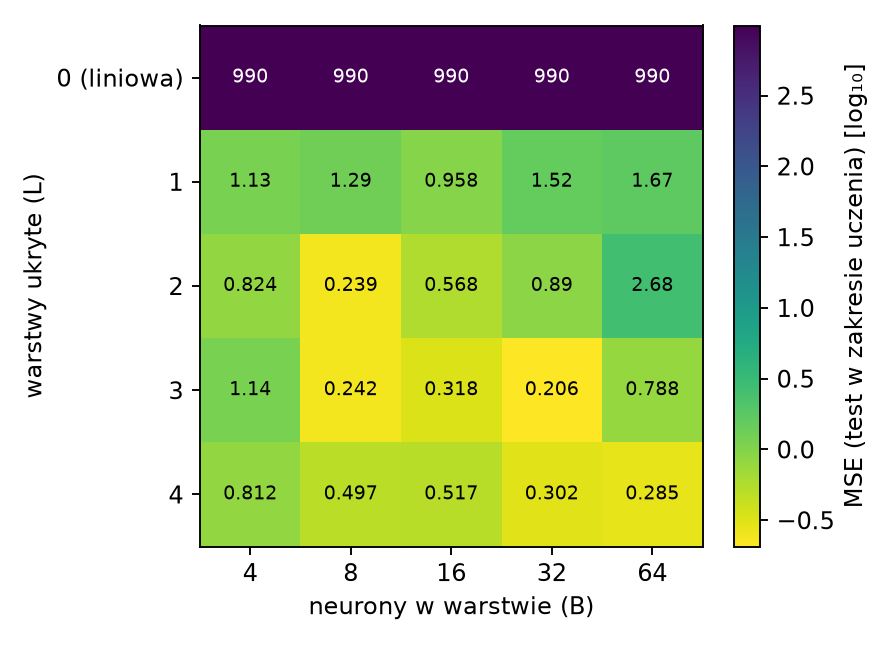
\includegraphics[width=0.7\linewidth]{figures/cube/arch_heatmap_test_in_mse.png}
  \caption{cube: MSE (test w zakresie uczenia) (mediana) w zależności od liczby warstw ukrytych $L$ i neuronów w warstwie $B$.}
  \label{fig:cube:arch_heatmap_test_in_mse}
\end{figure}

\begin{figure}[htbp]
  \centering
  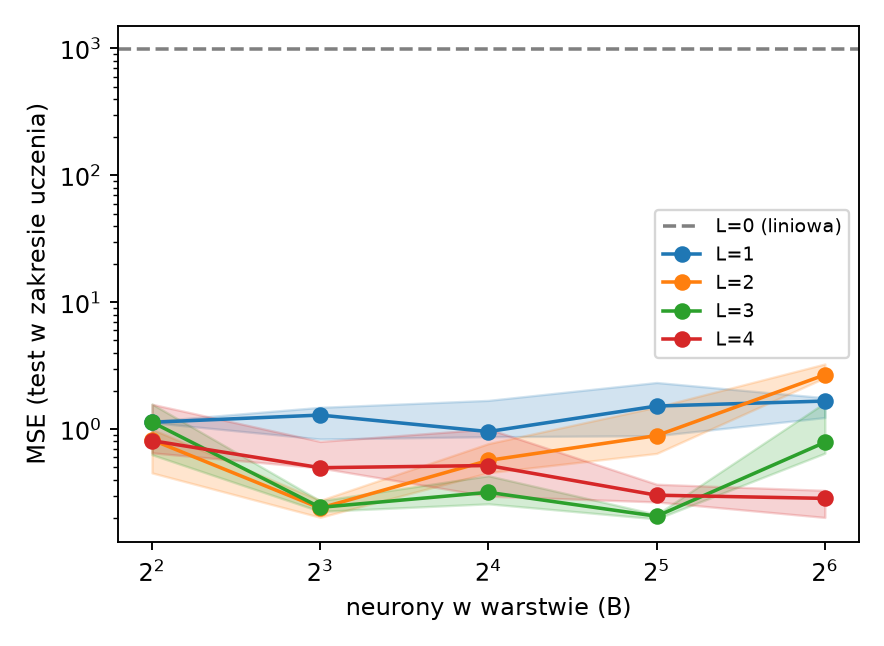
\includegraphics[width=0.7\linewidth]{figures/cube/arch_lines_test_in_mse.png}
  \caption{cube: MSE (test w zakresie uczenia) w zależności od $B$ dla każdej liczby warstw $L$ (mediana i kwartyle po ziarnach).}
  \label{fig:cube:arch_lines_test_in_mse}
\end{figure}

\begin{figure}[htbp]
  \centering
  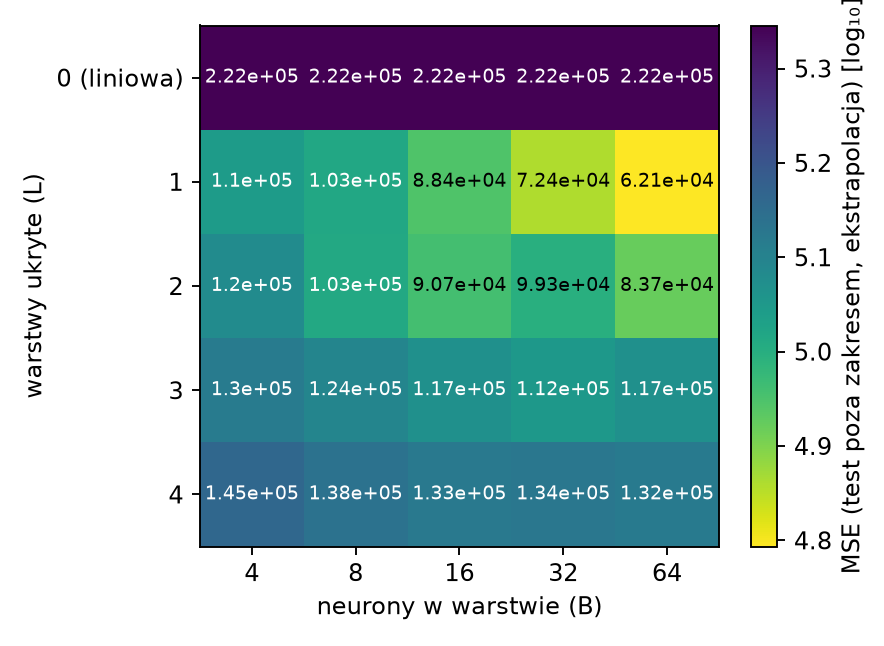
\includegraphics[width=0.7\linewidth]{figures/cube/arch_heatmap_test_out_mse.png}
  \caption{cube: MSE (test poza zakresem, ekstrapolacja) (mediana) w zależności od liczby warstw ukrytych $L$ i neuronów w warstwie $B$.}
  \label{fig:cube:arch_heatmap_test_out_mse}
\end{figure}

\begin{figure}[htbp]
  \centering
  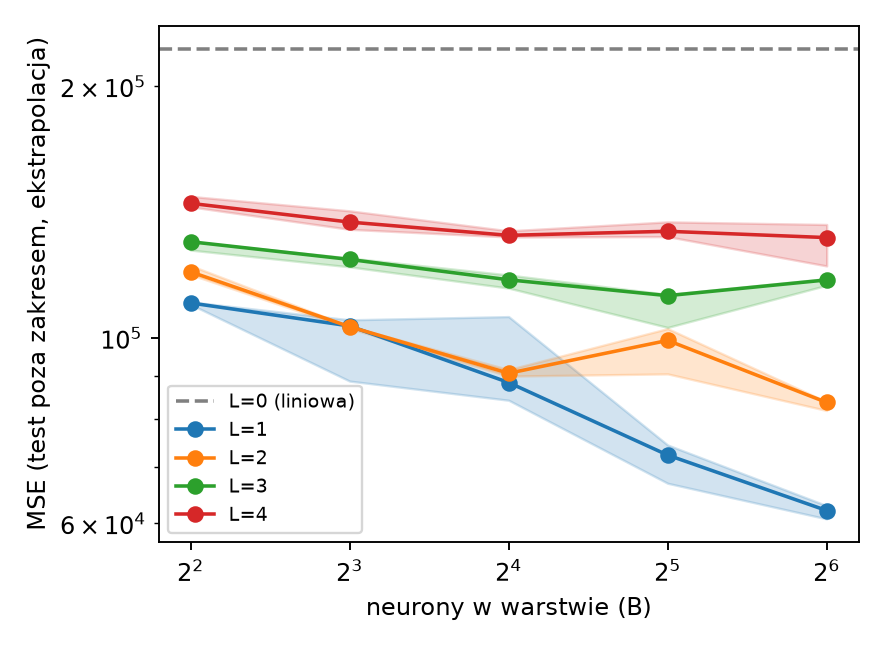
\includegraphics[width=0.7\linewidth]{figures/cube/arch_lines_test_out_mse.png}
  \caption{cube: MSE (test poza zakresem, ekstrapolacja) w zależności od $B$ dla każdej liczby warstw $L$ (mediana i kwartyle po ziarnach).}
  \label{fig:cube:arch_lines_test_out_mse}
\end{figure}

\begin{figure}[htbp]
  \centering
  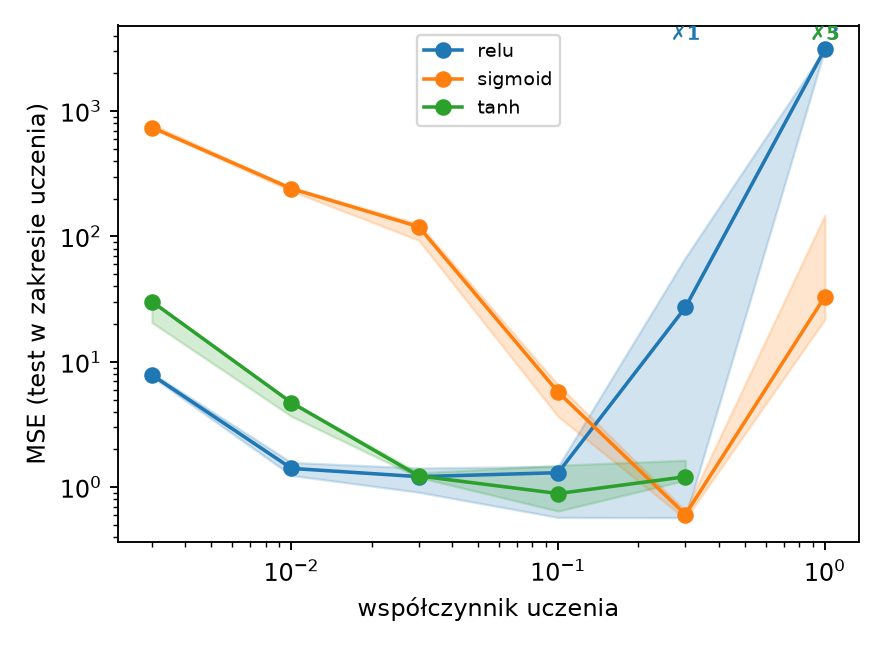
\includegraphics[width=0.7\linewidth]{figures/cube/activation_lr_test_in_mse.png}
  \caption{cube: MSE (test w zakresie uczenia) dla różnych funkcji aktywacji w zależności od współczynnika uczenia (mediana i kwartyle; liczba przy krzyżyku nad wykresem to liczba rozbieżnych ziaren).}
  \label{fig:cube:activation_lr_test_in_mse}
\end{figure}

\begin{figure}[htbp]
  \centering
  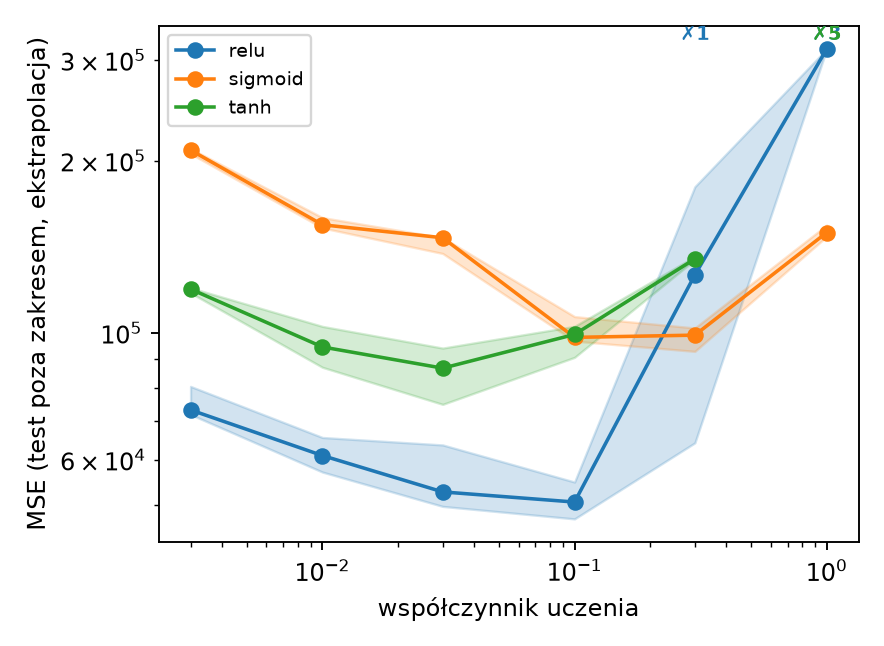
\includegraphics[width=0.7\linewidth]{figures/cube/activation_lr_test_out_mse.png}
  \caption{cube: MSE (test poza zakresem, ekstrapolacja) dla różnych funkcji aktywacji w zależności od współczynnika uczenia (mediana i kwartyle; liczba przy krzyżyku nad wykresem to liczba rozbieżnych ziaren).}
  \label{fig:cube:activation_lr_test_out_mse}
\end{figure}

\begin{figure}[htbp]
  \centering
  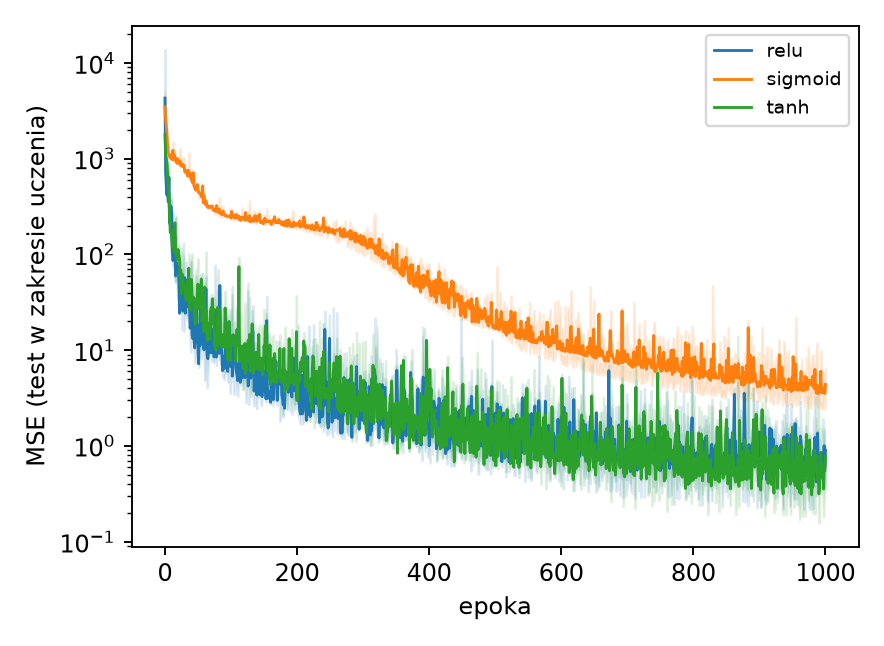
\includegraphics[width=0.7\linewidth]{figures/cube/activation_curve_test_in_mse.png}
  \caption{cube: przebieg MSE (test w zakresie uczenia) w trakcie uczenia dla różnych funkcji aktywacji (współczynnik uczenia 0.1).}
  \label{fig:cube:activation_curve_test_in_mse}
\end{figure}

\begin{figure}[htbp]
  \centering
  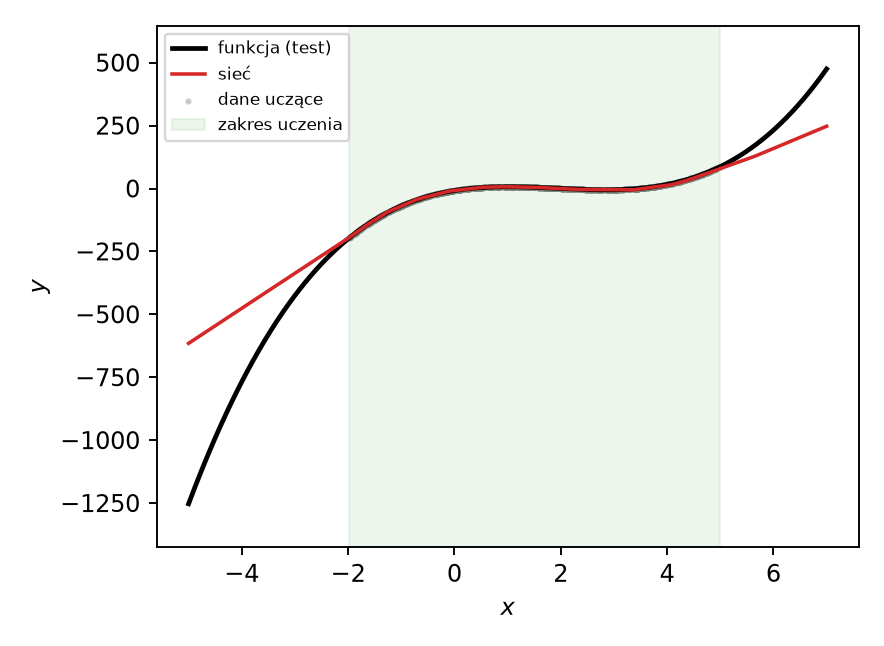
\includegraphics[width=0.7\linewidth]{figures/cube/predictions_relu.png}
  \caption{cube: funkcja nauczona przez sieć z aktywacją relu (ziarno 0) na całym zakresie testu; zielone tło to zakres danych uczących.}
  \label{fig:cube:predictions_relu}
\end{figure}

\begin{figure}[htbp]
  \centering
  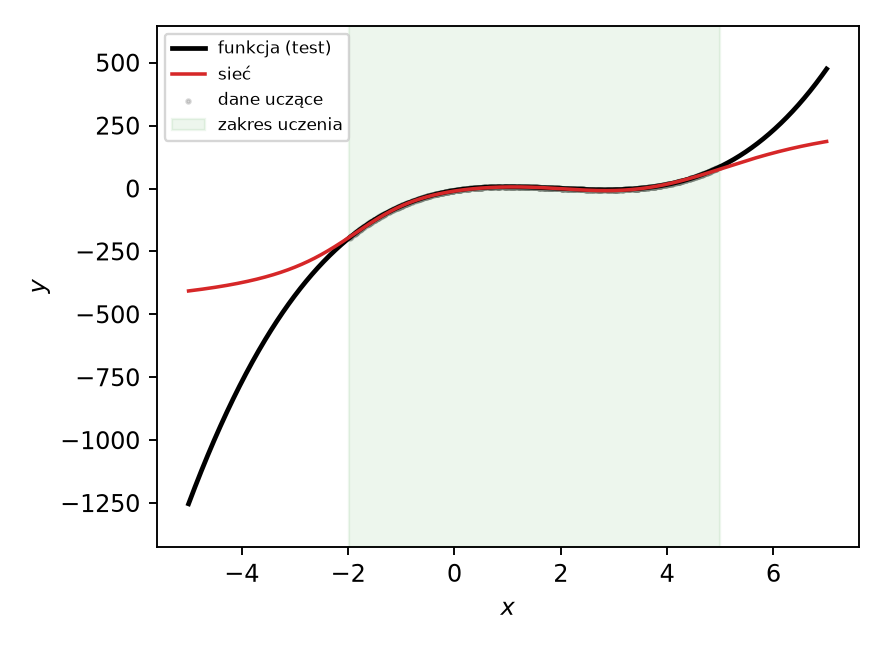
\includegraphics[width=0.7\linewidth]{figures/cube/predictions_sigmoid.png}
  \caption{cube: funkcja nauczona przez sieć z aktywacją sigmoid (ziarno 0) na całym zakresie testu; zielone tło to zakres danych uczących.}
  \label{fig:cube:predictions_sigmoid}
\end{figure}

\begin{figure}[htbp]
  \centering
  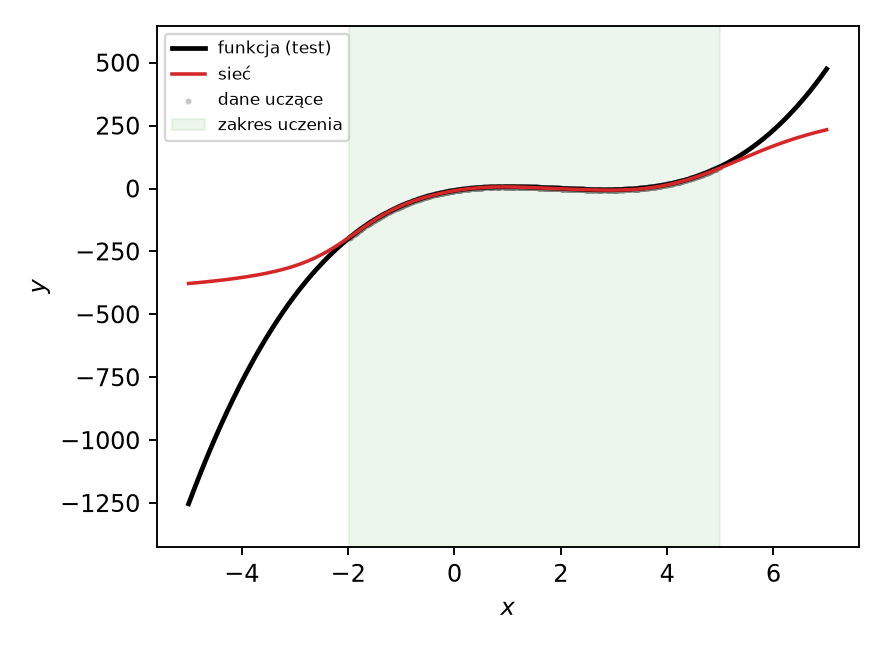
\includegraphics[width=0.7\linewidth]{figures/cube/predictions_tanh.png}
  \caption{cube: funkcja nauczona przez sieć z aktywacją tanh (ziarno 0) na całym zakresie testu; zielone tło to zakres danych uczących.}
  \label{fig:cube:predictions_tanh}
\end{figure}

\begin{figure}[htbp]
  \centering
  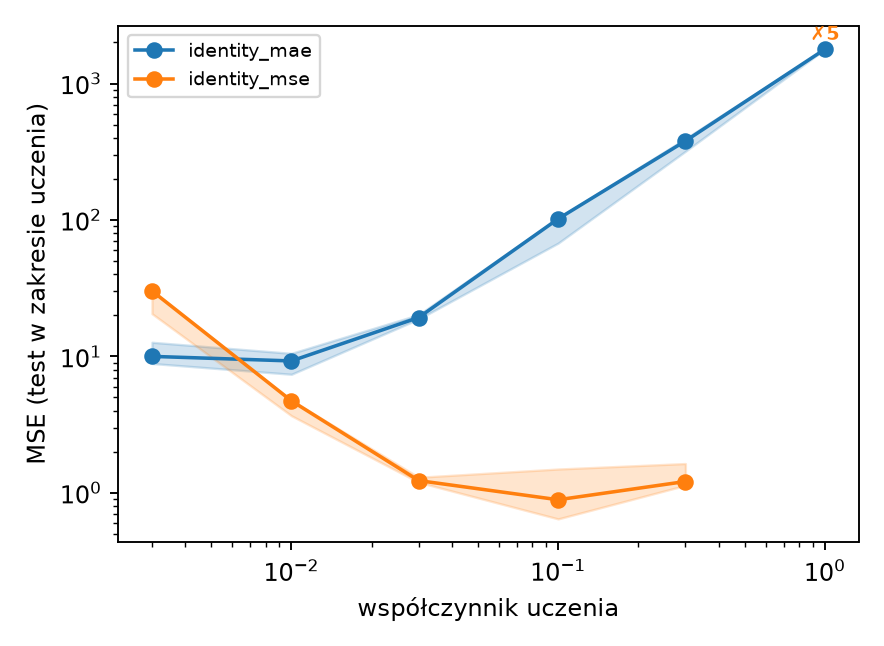
\includegraphics[width=0.7\linewidth]{figures/cube/loss_lr_test_in_mse.png}
  \caption{cube: MSE (test w zakresie uczenia) dla różnych funkcji kosztu w zależności od współczynnika uczenia (mediana i kwartyle; liczba przy krzyżyku nad wykresem to liczba rozbieżnych ziaren).}
  \label{fig:cube:loss_lr_test_in_mse}
\end{figure}

\begin{figure}[htbp]
  \centering
  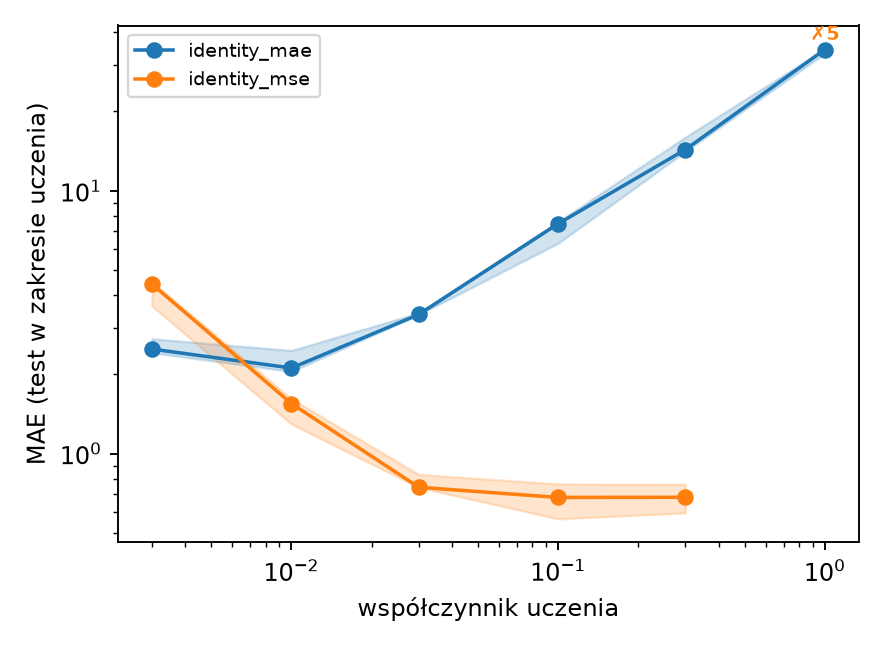
\includegraphics[width=0.7\linewidth]{figures/cube/loss_lr_test_in_mae.png}
  \caption{cube: MAE (test w zakresie uczenia) dla różnych funkcji kosztu w zależności od współczynnika uczenia (mediana i kwartyle; liczba przy krzyżyku nad wykresem to liczba rozbieżnych ziaren).}
  \label{fig:cube:loss_lr_test_in_mae}
\end{figure}

\begin{figure}[htbp]
  \centering
  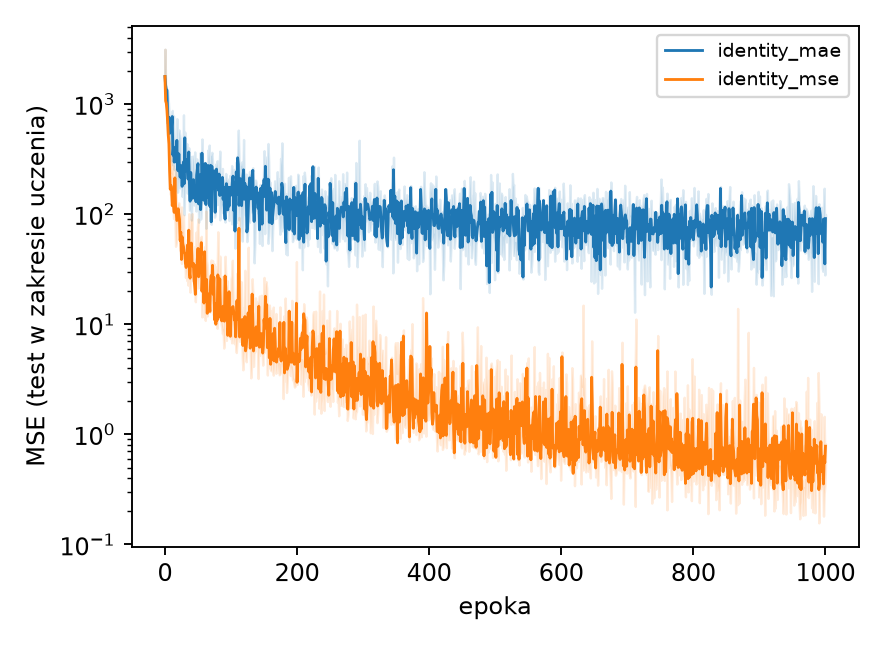
\includegraphics[width=0.7\linewidth]{figures/cube/loss_curve_test_in_mse.png}
  \caption{cube: przebieg MSE (test w zakresie uczenia) w trakcie uczenia dla różnych funkcji kosztu (współczynnik uczenia 0.1).}
  \label{fig:cube:loss_curve_test_in_mse}
\end{figure}

\begin{figure}[htbp]
  \centering
  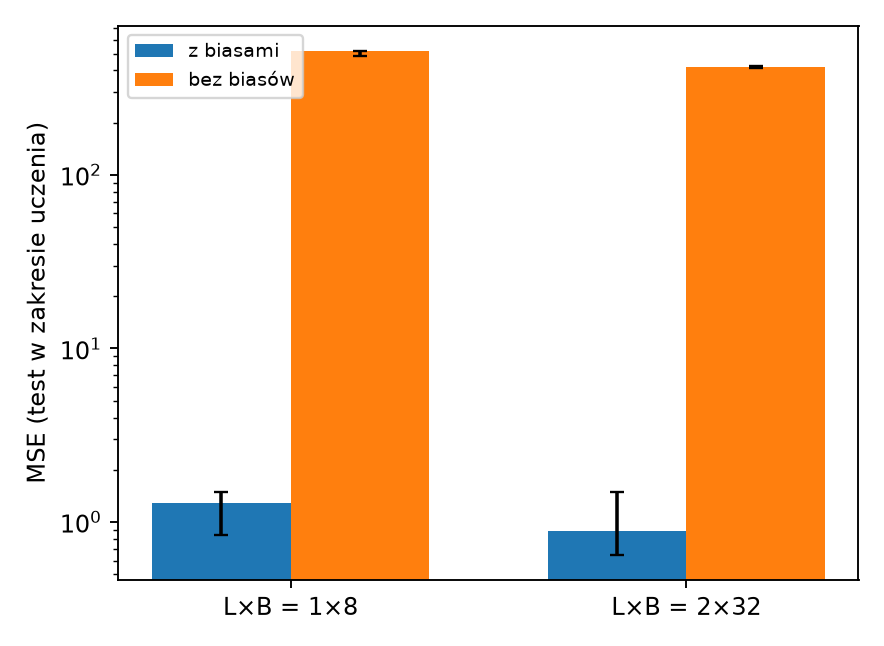
\includegraphics[width=0.7\linewidth]{figures/cube/bias.png}
  \caption{cube: MSE (test w zakresie uczenia) sieci z biasami i bez biasów.}
  \label{fig:cube:bias}
\end{figure}

\begin{figure}[htbp]
  \centering
  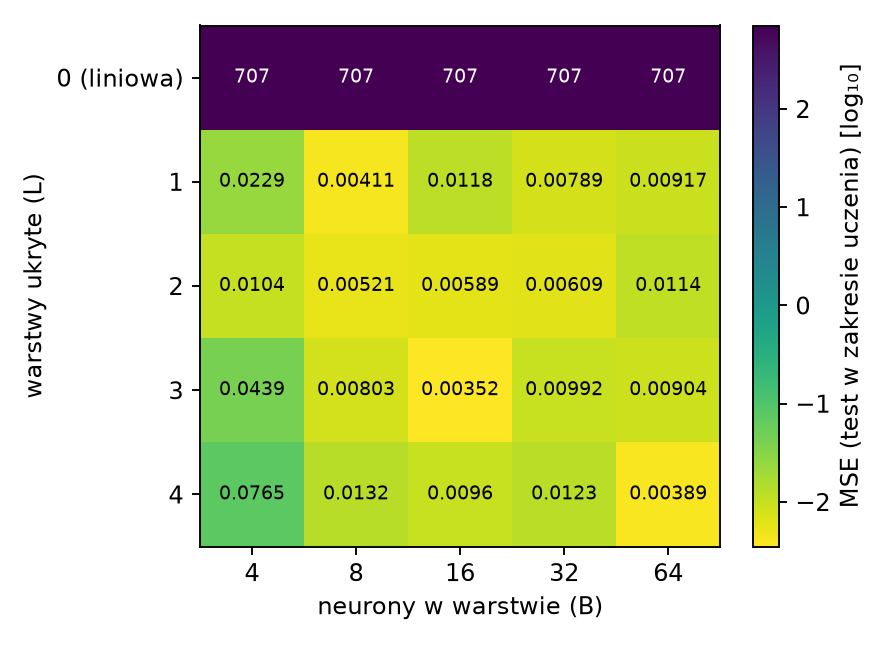
\includegraphics[width=0.7\linewidth]{figures/activation/arch_heatmap_test_in_mse.png}
  \caption{activation: MSE (test w zakresie uczenia) (mediana) w zależności od liczby warstw ukrytych $L$ i neuronów w warstwie $B$.}
  \label{fig:activation:arch_heatmap_test_in_mse}
\end{figure}

\begin{figure}[htbp]
  \centering
  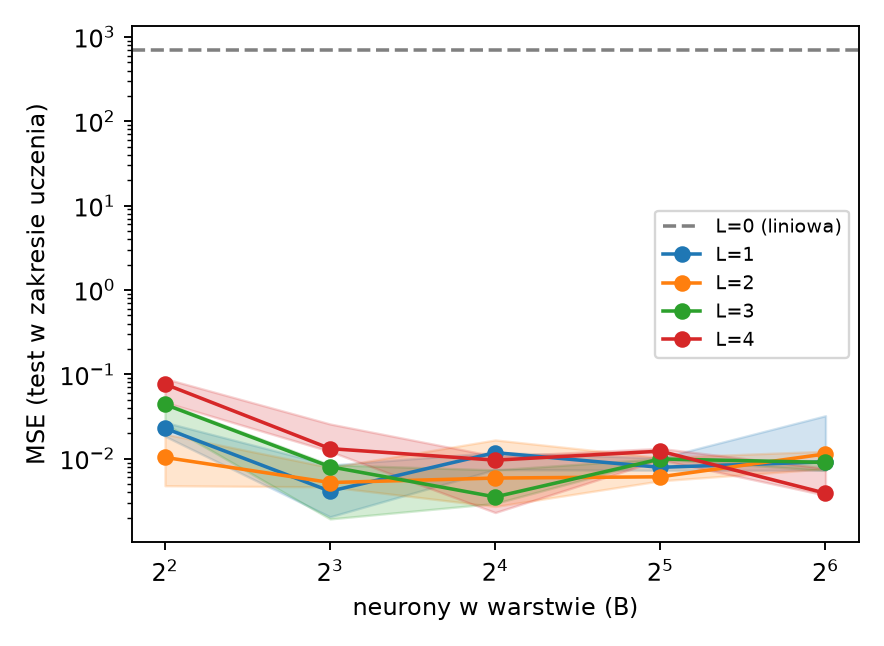
\includegraphics[width=0.7\linewidth]{figures/activation/arch_lines_test_in_mse.png}
  \caption{activation: MSE (test w zakresie uczenia) w zależności od $B$ dla każdej liczby warstw $L$ (mediana i kwartyle po ziarnach).}
  \label{fig:activation:arch_lines_test_in_mse}
\end{figure}

\begin{figure}[htbp]
  \centering
  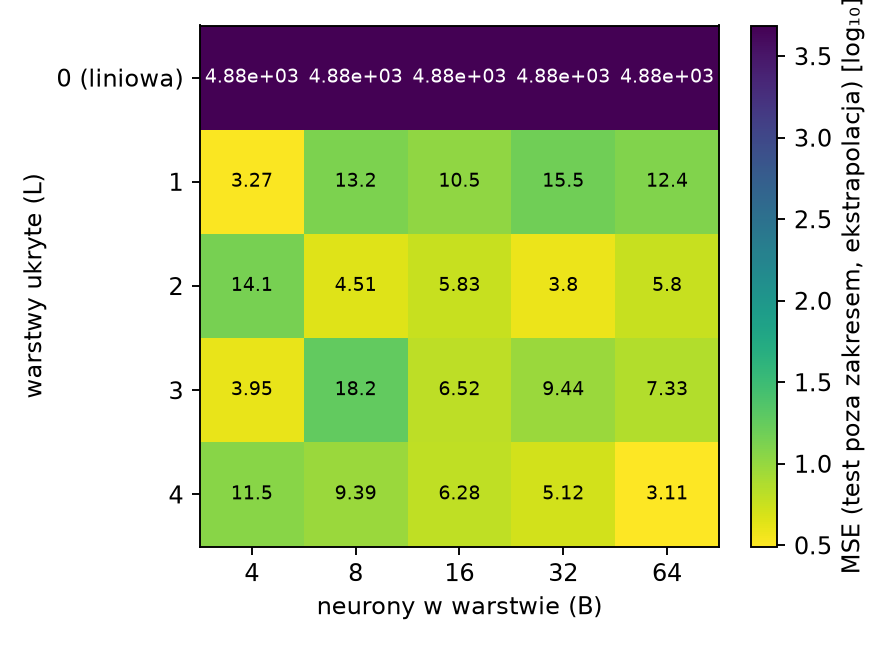
\includegraphics[width=0.7\linewidth]{figures/activation/arch_heatmap_test_out_mse.png}
  \caption{activation: MSE (test poza zakresem, ekstrapolacja) (mediana) w zależności od liczby warstw ukrytych $L$ i neuronów w warstwie $B$.}
  \label{fig:activation:arch_heatmap_test_out_mse}
\end{figure}

\begin{figure}[htbp]
  \centering
  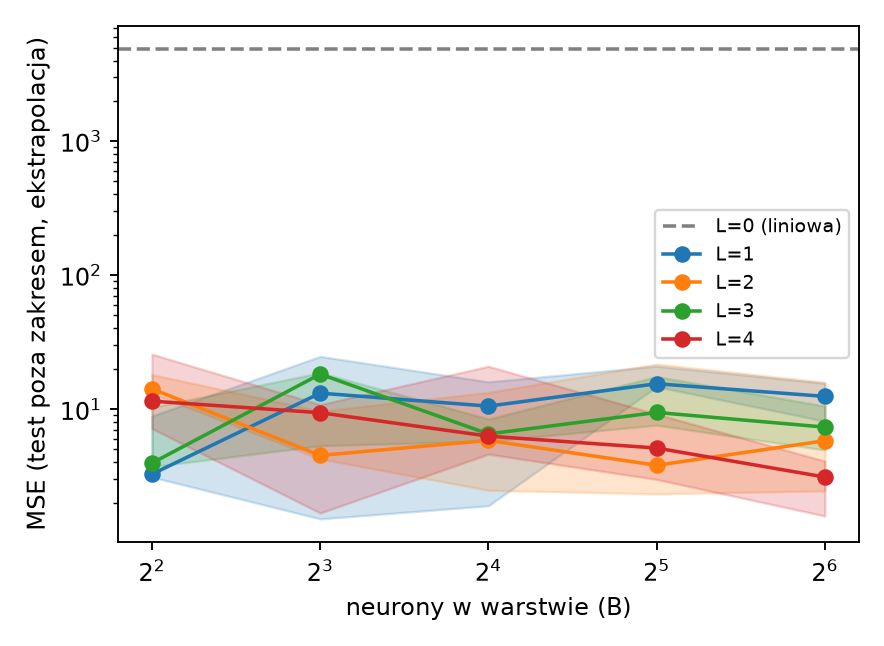
\includegraphics[width=0.7\linewidth]{figures/activation/arch_lines_test_out_mse.png}
  \caption{activation: MSE (test poza zakresem, ekstrapolacja) w zależności od $B$ dla każdej liczby warstw $L$ (mediana i kwartyle po ziarnach).}
  \label{fig:activation:arch_lines_test_out_mse}
\end{figure}

\begin{figure}[htbp]
  \centering
  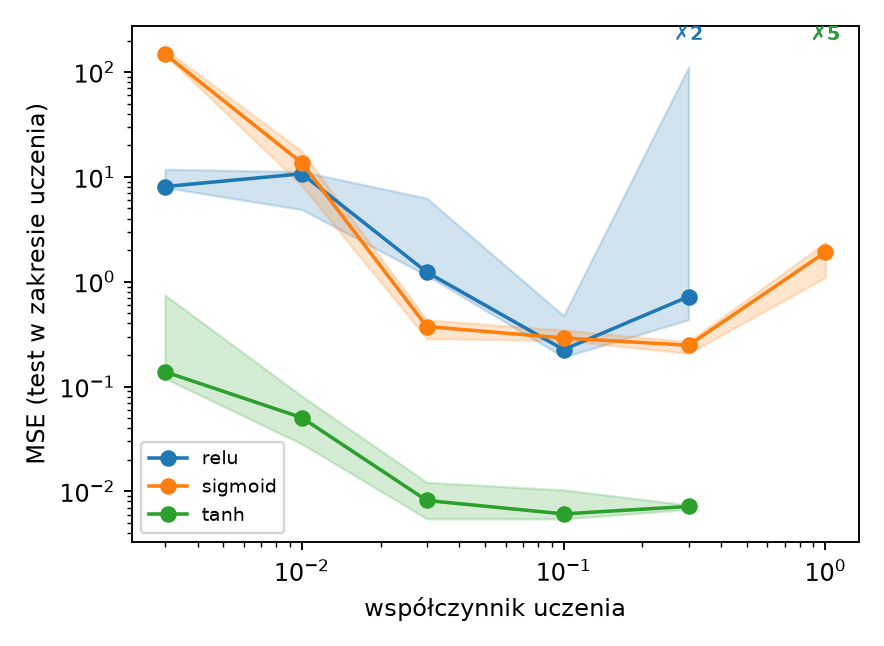
\includegraphics[width=0.7\linewidth]{figures/activation/activation_lr_test_in_mse.png}
  \caption{activation: MSE (test w zakresie uczenia) dla różnych funkcji aktywacji w zależności od współczynnika uczenia (mediana i kwartyle; liczba przy krzyżyku nad wykresem to liczba rozbieżnych ziaren).}
  \label{fig:activation:activation_lr_test_in_mse}
\end{figure}

\begin{figure}[htbp]
  \centering
  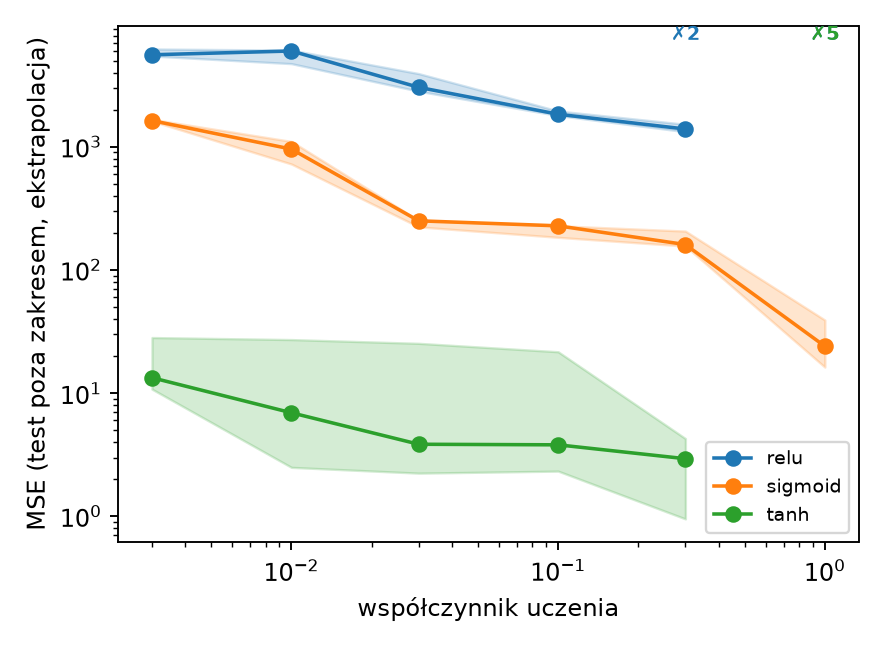
\includegraphics[width=0.7\linewidth]{figures/activation/activation_lr_test_out_mse.png}
  \caption{activation: MSE (test poza zakresem, ekstrapolacja) dla różnych funkcji aktywacji w zależności od współczynnika uczenia (mediana i kwartyle; liczba przy krzyżyku nad wykresem to liczba rozbieżnych ziaren).}
  \label{fig:activation:activation_lr_test_out_mse}
\end{figure}

\begin{figure}[htbp]
  \centering
  \includegraphics[width=0.7\linewidth]{figures/activation/activation_curve_test_in_mse.png}
  \caption{activation: przebieg MSE (test w zakresie uczenia) w trakcie uczenia dla różnych funkcji aktywacji (współczynnik uczenia 0.1).}
  \label{fig:activation:activation_curve_test_in_mse}
\end{figure}

\begin{figure}[htbp]
  \centering
  \includegraphics[width=0.7\linewidth]{figures/activation/predictions_relu.png}
  \caption{activation: funkcja nauczona przez sieć z aktywacją relu (ziarno 0) na całym zakresie testu; zielone tło to zakres danych uczących.}
  \label{fig:activation:predictions_relu}
\end{figure}

\begin{figure}[htbp]
  \centering
  \includegraphics[width=0.7\linewidth]{figures/activation/predictions_sigmoid.png}
  \caption{activation: funkcja nauczona przez sieć z aktywacją sigmoid (ziarno 0) na całym zakresie testu; zielone tło to zakres danych uczących.}
  \label{fig:activation:predictions_sigmoid}
\end{figure}

\begin{figure}[htbp]
  \centering
  \includegraphics[width=0.7\linewidth]{figures/activation/predictions_tanh.png}
  \caption{activation: funkcja nauczona przez sieć z aktywacją tanh (ziarno 0) na całym zakresie testu; zielone tło to zakres danych uczących.}
  \label{fig:activation:predictions_tanh}
\end{figure}

\begin{figure}[htbp]
  \centering
  \includegraphics[width=0.7\linewidth]{figures/activation/loss_lr_test_in_mse.png}
  \caption{activation: MSE (test w zakresie uczenia) dla różnych funkcji kosztu w zależności od współczynnika uczenia (mediana i kwartyle; liczba przy krzyżyku nad wykresem to liczba rozbieżnych ziaren).}
  \label{fig:activation:loss_lr_test_in_mse}
\end{figure}

\begin{figure}[htbp]
  \centering
  \includegraphics[width=0.7\linewidth]{figures/activation/loss_lr_test_in_mae.png}
  \caption{activation: MAE (test w zakresie uczenia) dla różnych funkcji kosztu w zależności od współczynnika uczenia (mediana i kwartyle; liczba przy krzyżyku nad wykresem to liczba rozbieżnych ziaren).}
  \label{fig:activation:loss_lr_test_in_mae}
\end{figure}

\begin{figure}[htbp]
  \centering
  \includegraphics[width=0.7\linewidth]{figures/activation/loss_curve_test_in_mse.png}
  \caption{activation: przebieg MSE (test w zakresie uczenia) w trakcie uczenia dla różnych funkcji kosztu (współczynnik uczenia 0.1).}
  \label{fig:activation:loss_curve_test_in_mse}
\end{figure}

\begin{figure}[htbp]
  \centering
  \includegraphics[width=0.7\linewidth]{figures/activation/bias.png}
  \caption{activation: MSE (test w zakresie uczenia) sieci z biasami i bez biasów.}
  \label{fig:activation:bias}
\end{figure}

\begin{figure}[htbp]
  \centering
  \includegraphics[width=0.7\linewidth]{figures/mnist/arch_heatmap_test_accuracy.png}
  \caption{MNIST: accuracy (test) (mediana) w zależności od liczby warstw ukrytych $L$ i neuronów w warstwie $B$.}
  \label{fig:mnist:arch_heatmap_test_accuracy}
\end{figure}

\begin{figure}[htbp]
  \centering
  \includegraphics[width=0.7\linewidth]{figures/mnist/arch_lines_test_accuracy.png}
  \caption{MNIST: accuracy (test) w zależności od $B$ dla każdej liczby warstw $L$ (mediana i kwartyle po ziarnach).}
  \label{fig:mnist:arch_lines_test_accuracy}
\end{figure}

\begin{figure}[htbp]
  \centering
  \includegraphics[width=0.7\linewidth]{figures/mnist/time_per_epoch.png}
  \caption{MNIST: czas jednej epoki (uczenie i ewaluacja, jeden wątek) w zależności od architektury.}
  \label{fig:mnist:time_per_epoch}
\end{figure}

\begin{figure}[htbp]
  \centering
  \includegraphics[width=0.7\linewidth]{figures/mnist/activation_lr_test_accuracy.png}
  \caption{MNIST: accuracy (test) dla różnych funkcji aktywacji w zależności od współczynnika uczenia (mediana i kwartyle; liczba przy krzyżyku nad wykresem to liczba rozbieżnych ziaren).}
  \label{fig:mnist:activation_lr_test_accuracy}
\end{figure}

\begin{figure}[htbp]
  \centering
  \includegraphics[width=0.7\linewidth]{figures/mnist/activation_lr_test_macro_f1.png}
  \caption{MNIST: macro-F1 (test) dla różnych funkcji aktywacji w zależności od współczynnika uczenia (mediana i kwartyle; liczba przy krzyżyku nad wykresem to liczba rozbieżnych ziaren).}
  \label{fig:mnist:activation_lr_test_macro_f1}
\end{figure}

\begin{figure}[htbp]
  \centering
  \includegraphics[width=0.7\linewidth]{figures/mnist/activation_curve_test_accuracy.png}
  \caption{MNIST: przebieg accuracy (test) w trakcie uczenia dla różnych funkcji aktywacji (współczynnik uczenia 0.1).}
  \label{fig:mnist:activation_curve_test_accuracy}
\end{figure}

\begin{figure}[htbp]
  \centering
  \includegraphics[width=0.7\linewidth]{figures/mnist/activation_curve_test_cost.png}
  \caption{MNIST: przebieg koszt (test) w trakcie uczenia dla różnych funkcji aktywacji (współczynnik uczenia 0.1).}
  \label{fig:mnist:activation_curve_test_cost}
\end{figure}

\begin{figure}[htbp]
  \centering
  \includegraphics[width=0.7\linewidth]{figures/mnist/confusion_relu_128.png}
  \caption{MNIST: macierz pomyłek na zbiorze testowym, aktywacja relu, architektura 128, suma po 5 ziarnach (accuracy 0.979).}
  \label{fig:mnist:confusion_relu_128}
\end{figure}

\begin{figure}[htbp]
  \centering
  \includegraphics[width=0.7\linewidth]{figures/mnist/confusion_sigmoid_128.png}
  \caption{MNIST: macierz pomyłek na zbiorze testowym, aktywacja sigmoid, architektura 128, suma po 5 ziarnach (accuracy 0.961).}
  \label{fig:mnist:confusion_sigmoid_128}
\end{figure}

\begin{figure}[htbp]
  \centering
  \includegraphics[width=0.7\linewidth]{figures/mnist/confusion_tanh_128.png}
  \caption{MNIST: macierz pomyłek na zbiorze testowym, aktywacja tanh, architektura 128, suma po 5 ziarnach (accuracy 0.977).}
  \label{fig:mnist:confusion_tanh_128}
\end{figure}

\begin{figure}[htbp]
  \centering
  \includegraphics[width=0.7\linewidth]{figures/mnist/loss_lr_test_accuracy.png}
  \caption{MNIST: accuracy (test) dla różnych funkcji kosztu w zależności od współczynnika uczenia (mediana i kwartyle; liczba przy krzyżyku nad wykresem to liczba rozbieżnych ziaren).}
  \label{fig:mnist:loss_lr_test_accuracy}
\end{figure}

\begin{figure}[htbp]
  \centering
  \includegraphics[width=0.7\linewidth]{figures/mnist/loss_lr_test_macro_f1.png}
  \caption{MNIST: macro-F1 (test) dla różnych funkcji kosztu w zależności od współczynnika uczenia (mediana i kwartyle; liczba przy krzyżyku nad wykresem to liczba rozbieżnych ziaren).}
  \label{fig:mnist:loss_lr_test_macro_f1}
\end{figure}

\begin{figure}[htbp]
  \centering
  \includegraphics[width=0.7\linewidth]{figures/mnist/loss_curve_test_accuracy.png}
  \caption{MNIST: przebieg accuracy (test) w trakcie uczenia dla różnych funkcji kosztu (współczynnik uczenia 0.1).}
  \label{fig:mnist:loss_curve_test_accuracy}
\end{figure}

\begin{figure}[htbp]
  \centering
  \includegraphics[width=0.7\linewidth]{figures/mnist/bias.png}
  \caption{MNIST: accuracy (test) sieci z biasami i bez biasów.}
  \label{fig:mnist:bias}
\end{figure}
 or copy single blocks.

\begin{figure}[htbp]
  \centering
  \includegraphics[width=0.7\linewidth]{figures/simple/arch_heatmap_test_accuracy.png}
  \caption{simple: accuracy (test) (mediana) w zależności od liczby warstw ukrytych $L$ i neuronów w warstwie $B$.}
  \label{fig:simple:arch_heatmap_test_accuracy}
\end{figure}

\begin{figure}[htbp]
  \centering
  \includegraphics[width=0.7\linewidth]{figures/simple/arch_lines_test_accuracy.png}
  \caption{simple: accuracy (test) w zależności od $B$ dla każdej liczby warstw $L$ (mediana i kwartyle po ziarnach).}
  \label{fig:simple:arch_lines_test_accuracy}
\end{figure}

\begin{figure}[htbp]
  \centering
  \includegraphics[width=0.7\linewidth]{figures/simple/activation_lr_test_accuracy.png}
  \caption{simple: accuracy (test) dla różnych funkcji aktywacji w zależności od współczynnika uczenia (mediana i kwartyle; liczba przy krzyżyku nad wykresem to liczba rozbieżnych ziaren).}
  \label{fig:simple:activation_lr_test_accuracy}
\end{figure}

\begin{figure}[htbp]
  \centering
  \includegraphics[width=0.7\linewidth]{figures/simple/activation_lr_test_macro_f1.png}
  \caption{simple: macro-F1 (test) dla różnych funkcji aktywacji w zależności od współczynnika uczenia (mediana i kwartyle; liczba przy krzyżyku nad wykresem to liczba rozbieżnych ziaren).}
  \label{fig:simple:activation_lr_test_macro_f1}
\end{figure}

\begin{figure}[htbp]
  \centering
  \includegraphics[width=0.7\linewidth]{figures/simple/activation_curve_test_accuracy.png}
  \caption{simple: przebieg accuracy (test) w trakcie uczenia dla różnych funkcji aktywacji (współczynnik uczenia 0.1).}
  \label{fig:simple:activation_curve_test_accuracy}
\end{figure}

\begin{figure}[htbp]
  \centering
  \includegraphics[width=0.7\linewidth]{figures/simple/activation_curve_test_cost.png}
  \caption{simple: przebieg koszt (test) w trakcie uczenia dla różnych funkcji aktywacji (współczynnik uczenia 0.1).}
  \label{fig:simple:activation_curve_test_cost}
\end{figure}

\begin{figure}[htbp]
  \centering
  \includegraphics[width=0.7\linewidth]{figures/simple/predictions_relu.png}
  \caption{simple: obszary decyzyjne sieci z aktywacją relu (ziarno 0). Punkty testowe w kolorze prawdziwej klasy, × oznacza pomyłkę (accuracy 0.995).}
  \label{fig:simple:predictions_relu}
\end{figure}

\begin{figure}[htbp]
  \centering
  \includegraphics[width=0.7\linewidth]{figures/simple/predictions_sigmoid.png}
  \caption{simple: obszary decyzyjne sieci z aktywacją sigmoid (ziarno 0). Punkty testowe w kolorze prawdziwej klasy, × oznacza pomyłkę (accuracy 0.997).}
  \label{fig:simple:predictions_sigmoid}
\end{figure}

\begin{figure}[htbp]
  \centering
  \includegraphics[width=0.7\linewidth]{figures/simple/predictions_tanh.png}
  \caption{simple: obszary decyzyjne sieci z aktywacją tanh (ziarno 0). Punkty testowe w kolorze prawdziwej klasy, × oznacza pomyłkę (accuracy 0.995).}
  \label{fig:simple:predictions_tanh}
\end{figure}

\begin{figure}[htbp]
  \centering
  \includegraphics[width=0.7\linewidth]{figures/simple/confusion_relu_32x32.png}
  \caption{simple: macierz pomyłek na zbiorze testowym, aktywacja relu, architektura 32x32, suma po 5 ziarnach (accuracy 0.991).}
  \label{fig:simple:confusion_relu_32x32}
\end{figure}

\begin{figure}[htbp]
  \centering
  \includegraphics[width=0.7\linewidth]{figures/simple/confusion_sigmoid_32x32.png}
  \caption{simple: macierz pomyłek na zbiorze testowym, aktywacja sigmoid, architektura 32x32, suma po 5 ziarnach (accuracy 0.996).}
  \label{fig:simple:confusion_sigmoid_32x32}
\end{figure}

\begin{figure}[htbp]
  \centering
  \includegraphics[width=0.7\linewidth]{figures/simple/confusion_tanh_32x32.png}
  \caption{simple: macierz pomyłek na zbiorze testowym, aktywacja tanh, architektura 32x32, suma po 5 ziarnach (accuracy 0.990).}
  \label{fig:simple:confusion_tanh_32x32}
\end{figure}

\begin{figure}[htbp]
  \centering
  \includegraphics[width=0.7\linewidth]{figures/simple/loss_lr_test_accuracy.png}
  \caption{simple: accuracy (test) dla różnych funkcji kosztu w zależności od współczynnika uczenia (mediana i kwartyle; liczba przy krzyżyku nad wykresem to liczba rozbieżnych ziaren).}
  \label{fig:simple:loss_lr_test_accuracy}
\end{figure}

\begin{figure}[htbp]
  \centering
  \includegraphics[width=0.7\linewidth]{figures/simple/loss_lr_test_macro_f1.png}
  \caption{simple: macro-F1 (test) dla różnych funkcji kosztu w zależności od współczynnika uczenia (mediana i kwartyle; liczba przy krzyżyku nad wykresem to liczba rozbieżnych ziaren).}
  \label{fig:simple:loss_lr_test_macro_f1}
\end{figure}

\begin{figure}[htbp]
  \centering
  \includegraphics[width=0.7\linewidth]{figures/simple/loss_curve_test_accuracy.png}
  \caption{simple: przebieg accuracy (test) w trakcie uczenia dla różnych funkcji kosztu (współczynnik uczenia 0.1).}
  \label{fig:simple:loss_curve_test_accuracy}
\end{figure}

\begin{figure}[htbp]
  \centering
  \includegraphics[width=0.7\linewidth]{figures/simple/bias.png}
  \caption{simple: accuracy (test) sieci z biasami i bez biasów.}
  \label{fig:simple:bias}
\end{figure}

\begin{figure}[htbp]
  \centering
  \includegraphics[width=0.7\linewidth]{figures/three_gauss/arch_heatmap_test_accuracy.png}
  \caption{three\_gauss: accuracy (test) (mediana) w zależności od liczby warstw ukrytych $L$ i neuronów w warstwie $B$.}
  \label{fig:three_gauss:arch_heatmap_test_accuracy}
\end{figure}

\begin{figure}[htbp]
  \centering
  \includegraphics[width=0.7\linewidth]{figures/three_gauss/arch_lines_test_accuracy.png}
  \caption{three\_gauss: accuracy (test) w zależności od $B$ dla każdej liczby warstw $L$ (mediana i kwartyle po ziarnach).}
  \label{fig:three_gauss:arch_lines_test_accuracy}
\end{figure}

\begin{figure}[htbp]
  \centering
  \includegraphics[width=0.7\linewidth]{figures/three_gauss/activation_lr_test_accuracy.png}
  \caption{three\_gauss: accuracy (test) dla różnych funkcji aktywacji w zależności od współczynnika uczenia (mediana i kwartyle; liczba przy krzyżyku nad wykresem to liczba rozbieżnych ziaren).}
  \label{fig:three_gauss:activation_lr_test_accuracy}
\end{figure}

\begin{figure}[htbp]
  \centering
  \includegraphics[width=0.7\linewidth]{figures/three_gauss/activation_lr_test_macro_f1.png}
  \caption{three\_gauss: macro-F1 (test) dla różnych funkcji aktywacji w zależności od współczynnika uczenia (mediana i kwartyle; liczba przy krzyżyku nad wykresem to liczba rozbieżnych ziaren).}
  \label{fig:three_gauss:activation_lr_test_macro_f1}
\end{figure}

\begin{figure}[htbp]
  \centering
  \includegraphics[width=0.7\linewidth]{figures/three_gauss/activation_curve_test_accuracy.png}
  \caption{three\_gauss: przebieg accuracy (test) w trakcie uczenia dla różnych funkcji aktywacji (współczynnik uczenia 0.1).}
  \label{fig:three_gauss:activation_curve_test_accuracy}
\end{figure}

\begin{figure}[htbp]
  \centering
  \includegraphics[width=0.7\linewidth]{figures/three_gauss/activation_curve_test_cost.png}
  \caption{three\_gauss: przebieg koszt (test) w trakcie uczenia dla różnych funkcji aktywacji (współczynnik uczenia 0.1).}
  \label{fig:three_gauss:activation_curve_test_cost}
\end{figure}

\begin{figure}[htbp]
  \centering
  \includegraphics[width=0.7\linewidth]{figures/three_gauss/predictions_relu.png}
  \caption{three\_gauss: obszary decyzyjne sieci z aktywacją relu (ziarno 0). Punkty testowe w kolorze prawdziwej klasy, × oznacza pomyłkę (accuracy 0.933).}
  \label{fig:three_gauss:predictions_relu}
\end{figure}

\begin{figure}[htbp]
  \centering
  \includegraphics[width=0.7\linewidth]{figures/three_gauss/predictions_sigmoid.png}
  \caption{three\_gauss: obszary decyzyjne sieci z aktywacją sigmoid (ziarno 0). Punkty testowe w kolorze prawdziwej klasy, × oznacza pomyłkę (accuracy 0.932).}
  \label{fig:three_gauss:predictions_sigmoid}
\end{figure}

\begin{figure}[htbp]
  \centering
  \includegraphics[width=0.7\linewidth]{figures/three_gauss/predictions_tanh.png}
  \caption{three\_gauss: obszary decyzyjne sieci z aktywacją tanh (ziarno 0). Punkty testowe w kolorze prawdziwej klasy, × oznacza pomyłkę (accuracy 0.933).}
  \label{fig:three_gauss:predictions_tanh}
\end{figure}

\begin{figure}[htbp]
  \centering
  \includegraphics[width=0.7\linewidth]{figures/three_gauss/confusion_relu_32x32.png}
  \caption{three\_gauss: macierz pomyłek na zbiorze testowym, aktywacja relu, architektura 32x32, suma po 5 ziarnach (accuracy 0.934).}
  \label{fig:three_gauss:confusion_relu_32x32}
\end{figure}

\begin{figure}[htbp]
  \centering
  \includegraphics[width=0.7\linewidth]{figures/three_gauss/confusion_sigmoid_32x32.png}
  \caption{three\_gauss: macierz pomyłek na zbiorze testowym, aktywacja sigmoid, architektura 32x32, suma po 5 ziarnach (accuracy 0.933).}
  \label{fig:three_gauss:confusion_sigmoid_32x32}
\end{figure}

\begin{figure}[htbp]
  \centering
  \includegraphics[width=0.7\linewidth]{figures/three_gauss/confusion_tanh_32x32.png}
  \caption{three\_gauss: macierz pomyłek na zbiorze testowym, aktywacja tanh, architektura 32x32, suma po 5 ziarnach (accuracy 0.935).}
  \label{fig:three_gauss:confusion_tanh_32x32}
\end{figure}

\begin{figure}[htbp]
  \centering
  \includegraphics[width=0.7\linewidth]{figures/three_gauss/loss_lr_test_accuracy.png}
  \caption{three\_gauss: accuracy (test) dla różnych funkcji kosztu w zależności od współczynnika uczenia (mediana i kwartyle; liczba przy krzyżyku nad wykresem to liczba rozbieżnych ziaren).}
  \label{fig:three_gauss:loss_lr_test_accuracy}
\end{figure}

\begin{figure}[htbp]
  \centering
  \includegraphics[width=0.7\linewidth]{figures/three_gauss/loss_lr_test_macro_f1.png}
  \caption{three\_gauss: macro-F1 (test) dla różnych funkcji kosztu w zależności od współczynnika uczenia (mediana i kwartyle; liczba przy krzyżyku nad wykresem to liczba rozbieżnych ziaren).}
  \label{fig:three_gauss:loss_lr_test_macro_f1}
\end{figure}

\begin{figure}[htbp]
  \centering
  \includegraphics[width=0.7\linewidth]{figures/three_gauss/loss_curve_test_accuracy.png}
  \caption{three\_gauss: przebieg accuracy (test) w trakcie uczenia dla różnych funkcji kosztu (współczynnik uczenia 0.1).}
  \label{fig:three_gauss:loss_curve_test_accuracy}
\end{figure}

\begin{figure}[htbp]
  \centering
  \includegraphics[width=0.7\linewidth]{figures/three_gauss/bias.png}
  \caption{three\_gauss: accuracy (test) sieci z biasami i bez biasów.}
  \label{fig:three_gauss:bias}
\end{figure}

\begin{figure}[htbp]
  \centering
  \includegraphics[width=0.7\linewidth]{figures/cube/arch_heatmap_test_in_mse.png}
  \caption{cube: MSE (test w zakresie uczenia) (mediana) w zależności od liczby warstw ukrytych $L$ i neuronów w warstwie $B$.}
  \label{fig:cube:arch_heatmap_test_in_mse}
\end{figure}

\begin{figure}[htbp]
  \centering
  \includegraphics[width=0.7\linewidth]{figures/cube/arch_lines_test_in_mse.png}
  \caption{cube: MSE (test w zakresie uczenia) w zależności od $B$ dla każdej liczby warstw $L$ (mediana i kwartyle po ziarnach).}
  \label{fig:cube:arch_lines_test_in_mse}
\end{figure}

\begin{figure}[htbp]
  \centering
  \includegraphics[width=0.7\linewidth]{figures/cube/arch_heatmap_test_out_mse.png}
  \caption{cube: MSE (test poza zakresem, ekstrapolacja) (mediana) w zależności od liczby warstw ukrytych $L$ i neuronów w warstwie $B$.}
  \label{fig:cube:arch_heatmap_test_out_mse}
\end{figure}

\begin{figure}[htbp]
  \centering
  \includegraphics[width=0.7\linewidth]{figures/cube/arch_lines_test_out_mse.png}
  \caption{cube: MSE (test poza zakresem, ekstrapolacja) w zależności od $B$ dla każdej liczby warstw $L$ (mediana i kwartyle po ziarnach).}
  \label{fig:cube:arch_lines_test_out_mse}
\end{figure}

\begin{figure}[htbp]
  \centering
  \includegraphics[width=0.7\linewidth]{figures/cube/activation_lr_test_in_mse.png}
  \caption{cube: MSE (test w zakresie uczenia) dla różnych funkcji aktywacji w zależności od współczynnika uczenia (mediana i kwartyle; liczba przy krzyżyku nad wykresem to liczba rozbieżnych ziaren).}
  \label{fig:cube:activation_lr_test_in_mse}
\end{figure}

\begin{figure}[htbp]
  \centering
  \includegraphics[width=0.7\linewidth]{figures/cube/activation_lr_test_out_mse.png}
  \caption{cube: MSE (test poza zakresem, ekstrapolacja) dla różnych funkcji aktywacji w zależności od współczynnika uczenia (mediana i kwartyle; liczba przy krzyżyku nad wykresem to liczba rozbieżnych ziaren).}
  \label{fig:cube:activation_lr_test_out_mse}
\end{figure}

\begin{figure}[htbp]
  \centering
  \includegraphics[width=0.7\linewidth]{figures/cube/activation_curve_test_in_mse.png}
  \caption{cube: przebieg MSE (test w zakresie uczenia) w trakcie uczenia dla różnych funkcji aktywacji (współczynnik uczenia 0.1).}
  \label{fig:cube:activation_curve_test_in_mse}
\end{figure}

\begin{figure}[htbp]
  \centering
  \includegraphics[width=0.7\linewidth]{figures/cube/predictions_relu.png}
  \caption{cube: funkcja nauczona przez sieć z aktywacją relu (ziarno 0) na całym zakresie testu; zielone tło to zakres danych uczących.}
  \label{fig:cube:predictions_relu}
\end{figure}

\begin{figure}[htbp]
  \centering
  \includegraphics[width=0.7\linewidth]{figures/cube/predictions_sigmoid.png}
  \caption{cube: funkcja nauczona przez sieć z aktywacją sigmoid (ziarno 0) na całym zakresie testu; zielone tło to zakres danych uczących.}
  \label{fig:cube:predictions_sigmoid}
\end{figure}

\begin{figure}[htbp]
  \centering
  \includegraphics[width=0.7\linewidth]{figures/cube/predictions_tanh.png}
  \caption{cube: funkcja nauczona przez sieć z aktywacją tanh (ziarno 0) na całym zakresie testu; zielone tło to zakres danych uczących.}
  \label{fig:cube:predictions_tanh}
\end{figure}

\begin{figure}[htbp]
  \centering
  \includegraphics[width=0.7\linewidth]{figures/cube/loss_lr_test_in_mse.png}
  \caption{cube: MSE (test w zakresie uczenia) dla różnych funkcji kosztu w zależności od współczynnika uczenia (mediana i kwartyle; liczba przy krzyżyku nad wykresem to liczba rozbieżnych ziaren).}
  \label{fig:cube:loss_lr_test_in_mse}
\end{figure}

\begin{figure}[htbp]
  \centering
  \includegraphics[width=0.7\linewidth]{figures/cube/loss_lr_test_in_mae.png}
  \caption{cube: MAE (test w zakresie uczenia) dla różnych funkcji kosztu w zależności od współczynnika uczenia (mediana i kwartyle; liczba przy krzyżyku nad wykresem to liczba rozbieżnych ziaren).}
  \label{fig:cube:loss_lr_test_in_mae}
\end{figure}

\begin{figure}[htbp]
  \centering
  \includegraphics[width=0.7\linewidth]{figures/cube/loss_curve_test_in_mse.png}
  \caption{cube: przebieg MSE (test w zakresie uczenia) w trakcie uczenia dla różnych funkcji kosztu (współczynnik uczenia 0.1).}
  \label{fig:cube:loss_curve_test_in_mse}
\end{figure}

\begin{figure}[htbp]
  \centering
  \includegraphics[width=0.7\linewidth]{figures/cube/bias.png}
  \caption{cube: MSE (test w zakresie uczenia) sieci z biasami i bez biasów.}
  \label{fig:cube:bias}
\end{figure}

\begin{figure}[htbp]
  \centering
  \includegraphics[width=0.7\linewidth]{figures/activation/arch_heatmap_test_in_mse.png}
  \caption{activation: MSE (test w zakresie uczenia) (mediana) w zależności od liczby warstw ukrytych $L$ i neuronów w warstwie $B$.}
  \label{fig:activation:arch_heatmap_test_in_mse}
\end{figure}

\begin{figure}[htbp]
  \centering
  \includegraphics[width=0.7\linewidth]{figures/activation/arch_lines_test_in_mse.png}
  \caption{activation: MSE (test w zakresie uczenia) w zależności od $B$ dla każdej liczby warstw $L$ (mediana i kwartyle po ziarnach).}
  \label{fig:activation:arch_lines_test_in_mse}
\end{figure}

\begin{figure}[htbp]
  \centering
  \includegraphics[width=0.7\linewidth]{figures/activation/arch_heatmap_test_out_mse.png}
  \caption{activation: MSE (test poza zakresem, ekstrapolacja) (mediana) w zależności od liczby warstw ukrytych $L$ i neuronów w warstwie $B$.}
  \label{fig:activation:arch_heatmap_test_out_mse}
\end{figure}

\begin{figure}[htbp]
  \centering
  \includegraphics[width=0.7\linewidth]{figures/activation/arch_lines_test_out_mse.png}
  \caption{activation: MSE (test poza zakresem, ekstrapolacja) w zależności od $B$ dla każdej liczby warstw $L$ (mediana i kwartyle po ziarnach).}
  \label{fig:activation:arch_lines_test_out_mse}
\end{figure}

\begin{figure}[htbp]
  \centering
  \includegraphics[width=0.7\linewidth]{figures/activation/activation_lr_test_in_mse.png}
  \caption{activation: MSE (test w zakresie uczenia) dla różnych funkcji aktywacji w zależności od współczynnika uczenia (mediana i kwartyle; liczba przy krzyżyku nad wykresem to liczba rozbieżnych ziaren).}
  \label{fig:activation:activation_lr_test_in_mse}
\end{figure}

\begin{figure}[htbp]
  \centering
  \includegraphics[width=0.7\linewidth]{figures/activation/activation_lr_test_out_mse.png}
  \caption{activation: MSE (test poza zakresem, ekstrapolacja) dla różnych funkcji aktywacji w zależności od współczynnika uczenia (mediana i kwartyle; liczba przy krzyżyku nad wykresem to liczba rozbieżnych ziaren).}
  \label{fig:activation:activation_lr_test_out_mse}
\end{figure}

\begin{figure}[htbp]
  \centering
  \includegraphics[width=0.7\linewidth]{figures/activation/activation_curve_test_in_mse.png}
  \caption{activation: przebieg MSE (test w zakresie uczenia) w trakcie uczenia dla różnych funkcji aktywacji (współczynnik uczenia 0.1).}
  \label{fig:activation:activation_curve_test_in_mse}
\end{figure}

\begin{figure}[htbp]
  \centering
  \includegraphics[width=0.7\linewidth]{figures/activation/predictions_relu.png}
  \caption{activation: funkcja nauczona przez sieć z aktywacją relu (ziarno 0) na całym zakresie testu; zielone tło to zakres danych uczących.}
  \label{fig:activation:predictions_relu}
\end{figure}

\begin{figure}[htbp]
  \centering
  \includegraphics[width=0.7\linewidth]{figures/activation/predictions_sigmoid.png}
  \caption{activation: funkcja nauczona przez sieć z aktywacją sigmoid (ziarno 0) na całym zakresie testu; zielone tło to zakres danych uczących.}
  \label{fig:activation:predictions_sigmoid}
\end{figure}

\begin{figure}[htbp]
  \centering
  \includegraphics[width=0.7\linewidth]{figures/activation/predictions_tanh.png}
  \caption{activation: funkcja nauczona przez sieć z aktywacją tanh (ziarno 0) na całym zakresie testu; zielone tło to zakres danych uczących.}
  \label{fig:activation:predictions_tanh}
\end{figure}

\begin{figure}[htbp]
  \centering
  \includegraphics[width=0.7\linewidth]{figures/activation/loss_lr_test_in_mse.png}
  \caption{activation: MSE (test w zakresie uczenia) dla różnych funkcji kosztu w zależności od współczynnika uczenia (mediana i kwartyle; liczba przy krzyżyku nad wykresem to liczba rozbieżnych ziaren).}
  \label{fig:activation:loss_lr_test_in_mse}
\end{figure}

\begin{figure}[htbp]
  \centering
  \includegraphics[width=0.7\linewidth]{figures/activation/loss_lr_test_in_mae.png}
  \caption{activation: MAE (test w zakresie uczenia) dla różnych funkcji kosztu w zależności od współczynnika uczenia (mediana i kwartyle; liczba przy krzyżyku nad wykresem to liczba rozbieżnych ziaren).}
  \label{fig:activation:loss_lr_test_in_mae}
\end{figure}

\begin{figure}[htbp]
  \centering
  \includegraphics[width=0.7\linewidth]{figures/activation/loss_curve_test_in_mse.png}
  \caption{activation: przebieg MSE (test w zakresie uczenia) w trakcie uczenia dla różnych funkcji kosztu (współczynnik uczenia 0.1).}
  \label{fig:activation:loss_curve_test_in_mse}
\end{figure}

\begin{figure}[htbp]
  \centering
  \includegraphics[width=0.7\linewidth]{figures/activation/bias.png}
  \caption{activation: MSE (test w zakresie uczenia) sieci z biasami i bez biasów.}
  \label{fig:activation:bias}
\end{figure}

\begin{figure}[htbp]
  \centering
  \includegraphics[width=0.7\linewidth]{figures/mnist/arch_heatmap_test_accuracy.png}
  \caption{MNIST: accuracy (test) (mediana) w zależności od liczby warstw ukrytych $L$ i neuronów w warstwie $B$.}
  \label{fig:mnist:arch_heatmap_test_accuracy}
\end{figure}

\begin{figure}[htbp]
  \centering
  \includegraphics[width=0.7\linewidth]{figures/mnist/arch_lines_test_accuracy.png}
  \caption{MNIST: accuracy (test) w zależności od $B$ dla każdej liczby warstw $L$ (mediana i kwartyle po ziarnach).}
  \label{fig:mnist:arch_lines_test_accuracy}
\end{figure}

\begin{figure}[htbp]
  \centering
  \includegraphics[width=0.7\linewidth]{figures/mnist/time_per_epoch.png}
  \caption{MNIST: czas jednej epoki (uczenie i ewaluacja, jeden wątek) w zależności od architektury.}
  \label{fig:mnist:time_per_epoch}
\end{figure}

\begin{figure}[htbp]
  \centering
  \includegraphics[width=0.7\linewidth]{figures/mnist/activation_lr_test_accuracy.png}
  \caption{MNIST: accuracy (test) dla różnych funkcji aktywacji w zależności od współczynnika uczenia (mediana i kwartyle; liczba przy krzyżyku nad wykresem to liczba rozbieżnych ziaren).}
  \label{fig:mnist:activation_lr_test_accuracy}
\end{figure}

\begin{figure}[htbp]
  \centering
  \includegraphics[width=0.7\linewidth]{figures/mnist/activation_lr_test_macro_f1.png}
  \caption{MNIST: macro-F1 (test) dla różnych funkcji aktywacji w zależności od współczynnika uczenia (mediana i kwartyle; liczba przy krzyżyku nad wykresem to liczba rozbieżnych ziaren).}
  \label{fig:mnist:activation_lr_test_macro_f1}
\end{figure}

\begin{figure}[htbp]
  \centering
  \includegraphics[width=0.7\linewidth]{figures/mnist/activation_curve_test_accuracy.png}
  \caption{MNIST: przebieg accuracy (test) w trakcie uczenia dla różnych funkcji aktywacji (współczynnik uczenia 0.1).}
  \label{fig:mnist:activation_curve_test_accuracy}
\end{figure}

\begin{figure}[htbp]
  \centering
  \includegraphics[width=0.7\linewidth]{figures/mnist/activation_curve_test_cost.png}
  \caption{MNIST: przebieg koszt (test) w trakcie uczenia dla różnych funkcji aktywacji (współczynnik uczenia 0.1).}
  \label{fig:mnist:activation_curve_test_cost}
\end{figure}

\begin{figure}[htbp]
  \centering
  \includegraphics[width=0.7\linewidth]{figures/mnist/confusion_relu_128.png}
  \caption{MNIST: macierz pomyłek na zbiorze testowym, aktywacja relu, architektura 128, suma po 5 ziarnach (accuracy 0.979).}
  \label{fig:mnist:confusion_relu_128}
\end{figure}

\begin{figure}[htbp]
  \centering
  \includegraphics[width=0.7\linewidth]{figures/mnist/confusion_sigmoid_128.png}
  \caption{MNIST: macierz pomyłek na zbiorze testowym, aktywacja sigmoid, architektura 128, suma po 5 ziarnach (accuracy 0.961).}
  \label{fig:mnist:confusion_sigmoid_128}
\end{figure}

\begin{figure}[htbp]
  \centering
  \includegraphics[width=0.7\linewidth]{figures/mnist/confusion_tanh_128.png}
  \caption{MNIST: macierz pomyłek na zbiorze testowym, aktywacja tanh, architektura 128, suma po 5 ziarnach (accuracy 0.977).}
  \label{fig:mnist:confusion_tanh_128}
\end{figure}

\begin{figure}[htbp]
  \centering
  \includegraphics[width=0.7\linewidth]{figures/mnist/loss_lr_test_accuracy.png}
  \caption{MNIST: accuracy (test) dla różnych funkcji kosztu w zależności od współczynnika uczenia (mediana i kwartyle; liczba przy krzyżyku nad wykresem to liczba rozbieżnych ziaren).}
  \label{fig:mnist:loss_lr_test_accuracy}
\end{figure}

\begin{figure}[htbp]
  \centering
  \includegraphics[width=0.7\linewidth]{figures/mnist/loss_lr_test_macro_f1.png}
  \caption{MNIST: macro-F1 (test) dla różnych funkcji kosztu w zależności od współczynnika uczenia (mediana i kwartyle; liczba przy krzyżyku nad wykresem to liczba rozbieżnych ziaren).}
  \label{fig:mnist:loss_lr_test_macro_f1}
\end{figure}

\begin{figure}[htbp]
  \centering
  \includegraphics[width=0.7\linewidth]{figures/mnist/loss_curve_test_accuracy.png}
  \caption{MNIST: przebieg accuracy (test) w trakcie uczenia dla różnych funkcji kosztu (współczynnik uczenia 0.1).}
  \label{fig:mnist:loss_curve_test_accuracy}
\end{figure}

\begin{figure}[htbp]
  \centering
  \includegraphics[width=0.7\linewidth]{figures/mnist/bias.png}
  \caption{MNIST: accuracy (test) sieci z biasami i bez biasów.}
  \label{fig:mnist:bias}
\end{figure}
